\documentclass{article}
\usepackage{standalone}
\usepackage{tikz}
\usepackage{siunitx}
\usepackage{float}
\usetikzlibrary{arrows,shapes}

%\usetikzlibrary{external}
%\tikzexternalize[prefix=figures/]

\begin{document}

\section{Basic plots}
\label{sec:basic}

\begin{figure}[H]
  \centering
  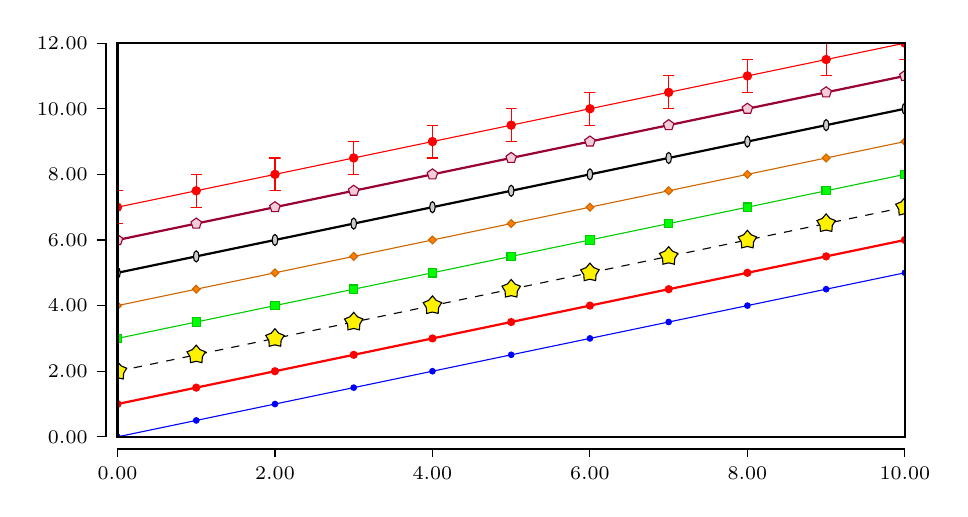
\begin{tikzpicture}[]
\begin{scope}[shift={(0.0,0.0)}]
\pgfsetxvec{\pgfpoint{1.0cm}{0cm}}
\pgfsetyvec{\pgfpoint{0cm}{0.41666666cm}}
\begin{scope}[shift={(0.0,0.0)}]
\begin{scope}[yshift=-0.15cm]
\draw[black] [shift={(0.0,0.0)}] (0,0) -- (0,-3pt) node[below]{ \scriptsize{\num[round-mode=places,round-precision=2]{0}}};
\draw[black] [shift={(2.0,0.0)}] (0,0) -- (0,-3pt) node[below]{ \scriptsize{\num[round-mode=places,round-precision=2]{2}}};
\draw[black] [shift={(4.0,0.0)}] (0,0) -- (0,-3pt) node[below]{ \scriptsize{\num[round-mode=places,round-precision=2]{4}}};
\draw[black] [shift={(6.0,0.0)}] (0,0) -- (0,-3pt) node[below]{ \scriptsize{\num[round-mode=places,round-precision=2]{6}}};
\draw[black] [shift={(8.0,0.0)}] (0,0) -- (0,-3pt) node[below]{ \scriptsize{\num[round-mode=places,round-precision=2]{8}}};
\draw[black] [shift={(10.0,0.0)}] (0,0) -- (0,-3pt) node[below]{ \scriptsize{\num[round-mode=places,round-precision=2]{10}}};
\end{scope}
\begin{scope}[xshift=-0.15cm]
\draw[black] [shift={(0.0,0.0)}] (0,0) -- (-3pt,0) node[left]{ \scriptsize{\num[round-mode=places,round-precision=2]{0}}};
\draw[black] [shift={(0.0,2.0)}] (0,0) -- (-3pt,0) node[left]{ \scriptsize{\num[round-mode=places,round-precision=2]{2}}};
\draw[black] [shift={(0.0,4.0)}] (0,0) -- (-3pt,0) node[left]{ \scriptsize{\num[round-mode=places,round-precision=2]{4}}};
\draw[black] [shift={(0.0,6.0)}] (0,0) -- (-3pt,0) node[left]{ \scriptsize{\num[round-mode=places,round-precision=2]{6}}};
\draw[black] [shift={(0.0,8.0)}] (0,0) -- (-3pt,0) node[left]{ \scriptsize{\num[round-mode=places,round-precision=2]{8}}};
\draw[black] [shift={(0.0,10.0)}] (0,0) -- (-3pt,0) node[left]{ \scriptsize{\num[round-mode=places,round-precision=2]{10}}};
\draw[black] [shift={(0.0,12.0)}] (0,0) -- (-3pt,0) node[left]{ \scriptsize{\num[round-mode=places,round-precision=2]{12}}};
\end{scope}
\end{scope}
\pgfsetxvec{\pgfpoint{1cm}{0cm}}
\pgfsetyvec{\pgfpoint{0cm}{1cm}}
\end{scope}
\begin{scope}[]
\clip (0.0,0.0) rectangle (10.0,5.0);
\begin{scope}[shift={(0.0,0.0)}]
\pgfsetxvec{\pgfpoint{1.0cm}{0cm}}
\pgfsetyvec{\pgfpoint{0cm}{0.41666666cm}}
\begin{scope}[shift={(0.0,0.0)}]
\begin{scope}[blue]
\pgfpathmoveto{ \pgfpointxy {0.0} {0.0}}
\pgfpathlineto{ \pgfpointxy {1.0} {0.5}}
\pgfpathlineto{ \pgfpointxy {2.0} {1.0}}
\pgfpathlineto{ \pgfpointxy {3.0} {1.5}}
\pgfpathlineto{ \pgfpointxy {4.0} {2.0}}
\pgfpathlineto{ \pgfpointxy {5.0} {2.5}}
\pgfpathlineto{ \pgfpointxy {6.0} {3.0}}
\pgfpathlineto{ \pgfpointxy {7.0} {3.5}}
\pgfpathlineto{ \pgfpointxy {8.0} {4.0}}
\pgfpathlineto{ \pgfpointxy {9.0} {4.5}}
\pgfpathlineto{ \pgfpointxy {10.0} {5.0}}
\pgfusepath{ stroke, }
\end{scope}
\node at (0.0,0.0) [circle,inner sep=0pt,minimum width =2pt,minimum height=2pt,fill=blue,draw=blue] {}; 
\node at (1.0,0.5) [circle,inner sep=0pt,minimum width =2pt,minimum height=2pt,fill=blue,draw=blue] {}; 
\node at (2.0,1.0) [circle,inner sep=0pt,minimum width =2pt,minimum height=2pt,fill=blue,draw=blue] {}; 
\node at (3.0,1.5) [circle,inner sep=0pt,minimum width =2pt,minimum height=2pt,fill=blue,draw=blue] {}; 
\node at (4.0,2.0) [circle,inner sep=0pt,minimum width =2pt,minimum height=2pt,fill=blue,draw=blue] {}; 
\node at (5.0,2.5) [circle,inner sep=0pt,minimum width =2pt,minimum height=2pt,fill=blue,draw=blue] {}; 
\node at (6.0,3.0) [circle,inner sep=0pt,minimum width =2pt,minimum height=2pt,fill=blue,draw=blue] {}; 
\node at (7.0,3.5) [circle,inner sep=0pt,minimum width =2pt,minimum height=2pt,fill=blue,draw=blue] {}; 
\node at (8.0,4.0) [circle,inner sep=0pt,minimum width =2pt,minimum height=2pt,fill=blue,draw=blue] {}; 
\node at (9.0,4.5) [circle,inner sep=0pt,minimum width =2pt,minimum height=2pt,fill=blue,draw=blue] {}; 
\node at (10.0,5.0) [circle,inner sep=0pt,minimum width =2pt,minimum height=2pt,fill=blue,draw=blue] {}; 
\begin{scope}[red,thick]
\pgfpathmoveto{ \pgfpointxy {0.0} {1.0}}
\pgfpathlineto{ \pgfpointxy {1.0} {1.5}}
\pgfpathlineto{ \pgfpointxy {2.0} {2.0}}
\pgfpathlineto{ \pgfpointxy {3.0} {2.5}}
\pgfpathlineto{ \pgfpointxy {4.0} {3.0}}
\pgfpathlineto{ \pgfpointxy {5.0} {3.5}}
\pgfpathlineto{ \pgfpointxy {6.0} {4.0}}
\pgfpathlineto{ \pgfpointxy {7.0} {4.5}}
\pgfpathlineto{ \pgfpointxy {8.0} {5.0}}
\pgfpathlineto{ \pgfpointxy {9.0} {5.5}}
\pgfpathlineto{ \pgfpointxy {10.0} {6.0}}
\pgfusepath{ stroke, }
\end{scope}
\node at (0.0,1.0) [circle,inner sep=0pt,minimum width =3pt,minimum height=3pt,fill=red] {}; 
\node at (1.0,1.5) [circle,inner sep=0pt,minimum width =3pt,minimum height=3pt,fill=red] {}; 
\node at (2.0,2.0) [circle,inner sep=0pt,minimum width =3pt,minimum height=3pt,fill=red] {}; 
\node at (3.0,2.5) [circle,inner sep=0pt,minimum width =3pt,minimum height=3pt,fill=red] {}; 
\node at (4.0,3.0) [circle,inner sep=0pt,minimum width =3pt,minimum height=3pt,fill=red] {}; 
\node at (5.0,3.5) [circle,inner sep=0pt,minimum width =3pt,minimum height=3pt,fill=red] {}; 
\node at (6.0,4.0) [circle,inner sep=0pt,minimum width =3pt,minimum height=3pt,fill=red] {}; 
\node at (7.0,4.5) [circle,inner sep=0pt,minimum width =3pt,minimum height=3pt,fill=red] {}; 
\node at (8.0,5.0) [circle,inner sep=0pt,minimum width =3pt,minimum height=3pt,fill=red] {}; 
\node at (9.0,5.5) [circle,inner sep=0pt,minimum width =3pt,minimum height=3pt,fill=red] {}; 
\node at (10.0,6.0) [circle,inner sep=0pt,minimum width =3pt,minimum height=3pt,fill=red] {}; 
\begin{scope}[black,dashed]
\pgfpathmoveto{ \pgfpointxy {0.0} {2.0}}
\pgfpathlineto{ \pgfpointxy {1.0} {2.5}}
\pgfpathlineto{ \pgfpointxy {2.0} {3.0}}
\pgfpathlineto{ \pgfpointxy {3.0} {3.5}}
\pgfpathlineto{ \pgfpointxy {4.0} {4.0}}
\pgfpathlineto{ \pgfpointxy {5.0} {4.5}}
\pgfpathlineto{ \pgfpointxy {6.0} {5.0}}
\pgfpathlineto{ \pgfpointxy {7.0} {5.5}}
\pgfpathlineto{ \pgfpointxy {8.0} {6.0}}
\pgfpathlineto{ \pgfpointxy {9.0} {6.5}}
\pgfpathlineto{ \pgfpointxy {10.0} {7.0}}
\pgfusepath{ stroke, }
\end{scope}
\node at (0.0,2.0) [star,star points=5,inner sep=0pt,minimum width =7pt,minimum height=7pt,draw=black,fill=yellow] {}; 
\node at (1.0,2.5) [star,star points=5,inner sep=0pt,minimum width =7pt,minimum height=7pt,draw=black,fill=yellow] {}; 
\node at (2.0,3.0) [star,star points=5,inner sep=0pt,minimum width =7pt,minimum height=7pt,draw=black,fill=yellow] {}; 
\node at (3.0,3.5) [star,star points=5,inner sep=0pt,minimum width =7pt,minimum height=7pt,draw=black,fill=yellow] {}; 
\node at (4.0,4.0) [star,star points=5,inner sep=0pt,minimum width =7pt,minimum height=7pt,draw=black,fill=yellow] {}; 
\node at (5.0,4.5) [star,star points=5,inner sep=0pt,minimum width =7pt,minimum height=7pt,draw=black,fill=yellow] {}; 
\node at (6.0,5.0) [star,star points=5,inner sep=0pt,minimum width =7pt,minimum height=7pt,draw=black,fill=yellow] {}; 
\node at (7.0,5.5) [star,star points=5,inner sep=0pt,minimum width =7pt,minimum height=7pt,draw=black,fill=yellow] {}; 
\node at (8.0,6.0) [star,star points=5,inner sep=0pt,minimum width =7pt,minimum height=7pt,draw=black,fill=yellow] {}; 
\node at (9.0,6.5) [star,star points=5,inner sep=0pt,minimum width =7pt,minimum height=7pt,draw=black,fill=yellow] {}; 
\node at (10.0,7.0) [star,star points=5,inner sep=0pt,minimum width =7pt,minimum height=7pt,draw=black,fill=yellow] {}; 
\begin{scope}[green!80!black]
\pgfpathmoveto{ \pgfpointxy {0.0} {3.0}}
\pgfpathlineto{ \pgfpointxy {1.0} {3.5}}
\pgfpathlineto{ \pgfpointxy {2.0} {4.0}}
\pgfpathlineto{ \pgfpointxy {3.0} {4.5}}
\pgfpathlineto{ \pgfpointxy {4.0} {5.0}}
\pgfpathlineto{ \pgfpointxy {5.0} {5.5}}
\pgfpathlineto{ \pgfpointxy {6.0} {6.0}}
\pgfpathlineto{ \pgfpointxy {7.0} {6.5}}
\pgfpathlineto{ \pgfpointxy {8.0} {7.0}}
\pgfpathlineto{ \pgfpointxy {9.0} {7.5}}
\pgfpathlineto{ \pgfpointxy {10.0} {8.0}}
\pgfusepath{ stroke, }
\end{scope}
\node at (0.0,3.0) [rectangle,inner sep=0pt,minimum width =3pt,minimum height=3pt,draw=green!80!black,fill=green] {}; 
\node at (1.0,3.5) [rectangle,inner sep=0pt,minimum width =3pt,minimum height=3pt,draw=green!80!black,fill=green] {}; 
\node at (2.0,4.0) [rectangle,inner sep=0pt,minimum width =3pt,minimum height=3pt,draw=green!80!black,fill=green] {}; 
\node at (3.0,4.5) [rectangle,inner sep=0pt,minimum width =3pt,minimum height=3pt,draw=green!80!black,fill=green] {}; 
\node at (4.0,5.0) [rectangle,inner sep=0pt,minimum width =3pt,minimum height=3pt,draw=green!80!black,fill=green] {}; 
\node at (5.0,5.5) [rectangle,inner sep=0pt,minimum width =3pt,minimum height=3pt,draw=green!80!black,fill=green] {}; 
\node at (6.0,6.0) [rectangle,inner sep=0pt,minimum width =3pt,minimum height=3pt,draw=green!80!black,fill=green] {}; 
\node at (7.0,6.5) [rectangle,inner sep=0pt,minimum width =3pt,minimum height=3pt,draw=green!80!black,fill=green] {}; 
\node at (8.0,7.0) [rectangle,inner sep=0pt,minimum width =3pt,minimum height=3pt,draw=green!80!black,fill=green] {}; 
\node at (9.0,7.5) [rectangle,inner sep=0pt,minimum width =3pt,minimum height=3pt,draw=green!80!black,fill=green] {}; 
\node at (10.0,8.0) [rectangle,inner sep=0pt,minimum width =3pt,minimum height=3pt,draw=green!80!black,fill=green] {}; 
\begin{scope}[orange!80!black]
\pgfpathmoveto{ \pgfpointxy {0.0} {4.0}}
\pgfpathlineto{ \pgfpointxy {1.0} {4.5}}
\pgfpathlineto{ \pgfpointxy {2.0} {5.0}}
\pgfpathlineto{ \pgfpointxy {3.0} {5.5}}
\pgfpathlineto{ \pgfpointxy {4.0} {6.0}}
\pgfpathlineto{ \pgfpointxy {5.0} {6.5}}
\pgfpathlineto{ \pgfpointxy {6.0} {7.0}}
\pgfpathlineto{ \pgfpointxy {7.0} {7.5}}
\pgfpathlineto{ \pgfpointxy {8.0} {8.0}}
\pgfpathlineto{ \pgfpointxy {9.0} {8.5}}
\pgfpathlineto{ \pgfpointxy {10.0} {9.0}}
\pgfusepath{ stroke, }
\end{scope}
\node at (0.0,4.0) [diamond,inner sep=0pt,minimum width =3pt,minimum height=3pt,draw=orange!80!black,fill=orange] {}; 
\node at (1.0,4.5) [diamond,inner sep=0pt,minimum width =3pt,minimum height=3pt,draw=orange!80!black,fill=orange] {}; 
\node at (2.0,5.0) [diamond,inner sep=0pt,minimum width =3pt,minimum height=3pt,draw=orange!80!black,fill=orange] {}; 
\node at (3.0,5.5) [diamond,inner sep=0pt,minimum width =3pt,minimum height=3pt,draw=orange!80!black,fill=orange] {}; 
\node at (4.0,6.0) [diamond,inner sep=0pt,minimum width =3pt,minimum height=3pt,draw=orange!80!black,fill=orange] {}; 
\node at (5.0,6.5) [diamond,inner sep=0pt,minimum width =3pt,minimum height=3pt,draw=orange!80!black,fill=orange] {}; 
\node at (6.0,7.0) [diamond,inner sep=0pt,minimum width =3pt,minimum height=3pt,draw=orange!80!black,fill=orange] {}; 
\node at (7.0,7.5) [diamond,inner sep=0pt,minimum width =3pt,minimum height=3pt,draw=orange!80!black,fill=orange] {}; 
\node at (8.0,8.0) [diamond,inner sep=0pt,minimum width =3pt,minimum height=3pt,draw=orange!80!black,fill=orange] {}; 
\node at (9.0,8.5) [diamond,inner sep=0pt,minimum width =3pt,minimum height=3pt,draw=orange!80!black,fill=orange] {}; 
\node at (10.0,9.0) [diamond,inner sep=0pt,minimum width =3pt,minimum height=3pt,draw=orange!80!black,fill=orange] {}; 
\begin{scope}[black,thick]
\pgfpathmoveto{ \pgfpointxy {0.0} {5.0}}
\pgfpathlineto{ \pgfpointxy {1.0} {5.5}}
\pgfpathlineto{ \pgfpointxy {2.0} {6.0}}
\pgfpathlineto{ \pgfpointxy {3.0} {6.5}}
\pgfpathlineto{ \pgfpointxy {4.0} {7.0}}
\pgfpathlineto{ \pgfpointxy {5.0} {7.5}}
\pgfpathlineto{ \pgfpointxy {6.0} {8.0}}
\pgfpathlineto{ \pgfpointxy {7.0} {8.5}}
\pgfpathlineto{ \pgfpointxy {8.0} {9.0}}
\pgfpathlineto{ \pgfpointxy {9.0} {9.5}}
\pgfpathlineto{ \pgfpointxy {10.0} {10.0}}
\pgfusepath{ stroke, }
\end{scope}
\node at (0.0,5.0) [ellipse,inner sep=0pt,minimum width =2pt,minimum height=4pt,draw=black,fill=black!20] {}; 
\node at (1.0,5.5) [ellipse,inner sep=0pt,minimum width =2pt,minimum height=4pt,draw=black,fill=black!20] {}; 
\node at (2.0,6.0) [ellipse,inner sep=0pt,minimum width =2pt,minimum height=4pt,draw=black,fill=black!20] {}; 
\node at (3.0,6.5) [ellipse,inner sep=0pt,minimum width =2pt,minimum height=4pt,draw=black,fill=black!20] {}; 
\node at (4.0,7.0) [ellipse,inner sep=0pt,minimum width =2pt,minimum height=4pt,draw=black,fill=black!20] {}; 
\node at (5.0,7.5) [ellipse,inner sep=0pt,minimum width =2pt,minimum height=4pt,draw=black,fill=black!20] {}; 
\node at (6.0,8.0) [ellipse,inner sep=0pt,minimum width =2pt,minimum height=4pt,draw=black,fill=black!20] {}; 
\node at (7.0,8.5) [ellipse,inner sep=0pt,minimum width =2pt,minimum height=4pt,draw=black,fill=black!20] {}; 
\node at (8.0,9.0) [ellipse,inner sep=0pt,minimum width =2pt,minimum height=4pt,draw=black,fill=black!20] {}; 
\node at (9.0,9.5) [ellipse,inner sep=0pt,minimum width =2pt,minimum height=4pt,draw=black,fill=black!20] {}; 
\node at (10.0,10.0) [ellipse,inner sep=0pt,minimum width =2pt,minimum height=4pt,draw=black,fill=black!20] {}; 
\begin{scope}[purple!80!black,thick]
\pgfpathmoveto{ \pgfpointxy {0.0} {6.0}}
\pgfpathlineto{ \pgfpointxy {1.0} {6.5}}
\pgfpathlineto{ \pgfpointxy {2.0} {7.0}}
\pgfpathlineto{ \pgfpointxy {3.0} {7.5}}
\pgfpathlineto{ \pgfpointxy {4.0} {8.0}}
\pgfpathlineto{ \pgfpointxy {5.0} {8.5}}
\pgfpathlineto{ \pgfpointxy {6.0} {9.0}}
\pgfpathlineto{ \pgfpointxy {7.0} {9.5}}
\pgfpathlineto{ \pgfpointxy {8.0} {10.0}}
\pgfpathlineto{ \pgfpointxy {9.0} {10.5}}
\pgfpathlineto{ \pgfpointxy {10.0} {11.0}}
\pgfusepath{ stroke, }
\end{scope}
\node at (0.0,6.0) [regular polygon,regular polygon sides=5,inner sep=0pt,minimum width =4pt,minimum height=4pt,draw=purple!80!black,fill=purple!20] {}; 
\node at (1.0,6.5) [regular polygon,regular polygon sides=5,inner sep=0pt,minimum width =4pt,minimum height=4pt,draw=purple!80!black,fill=purple!20] {}; 
\node at (2.0,7.0) [regular polygon,regular polygon sides=5,inner sep=0pt,minimum width =4pt,minimum height=4pt,draw=purple!80!black,fill=purple!20] {}; 
\node at (3.0,7.5) [regular polygon,regular polygon sides=5,inner sep=0pt,minimum width =4pt,minimum height=4pt,draw=purple!80!black,fill=purple!20] {}; 
\node at (4.0,8.0) [regular polygon,regular polygon sides=5,inner sep=0pt,minimum width =4pt,minimum height=4pt,draw=purple!80!black,fill=purple!20] {}; 
\node at (5.0,8.5) [regular polygon,regular polygon sides=5,inner sep=0pt,minimum width =4pt,minimum height=4pt,draw=purple!80!black,fill=purple!20] {}; 
\node at (6.0,9.0) [regular polygon,regular polygon sides=5,inner sep=0pt,minimum width =4pt,minimum height=4pt,draw=purple!80!black,fill=purple!20] {}; 
\node at (7.0,9.5) [regular polygon,regular polygon sides=5,inner sep=0pt,minimum width =4pt,minimum height=4pt,draw=purple!80!black,fill=purple!20] {}; 
\node at (8.0,10.0) [regular polygon,regular polygon sides=5,inner sep=0pt,minimum width =4pt,minimum height=4pt,draw=purple!80!black,fill=purple!20] {}; 
\node at (9.0,10.5) [regular polygon,regular polygon sides=5,inner sep=0pt,minimum width =4pt,minimum height=4pt,draw=purple!80!black,fill=purple!20] {}; 
\node at (10.0,11.0) [regular polygon,regular polygon sides=5,inner sep=0pt,minimum width =4pt,minimum height=4pt,draw=purple!80!black,fill=purple!20] {}; 
\begin{scope}[red]
\pgfpathmoveto{ \pgfpointxy {0.0} {7.0}}
\pgfpathlineto{ \pgfpointxy {1.0} {7.5}}
\pgfpathlineto{ \pgfpointxy {2.0} {8.0}}
\pgfpathlineto{ \pgfpointxy {3.0} {8.5}}
\pgfpathlineto{ \pgfpointxy {4.0} {9.0}}
\pgfpathlineto{ \pgfpointxy {5.0} {9.5}}
\pgfpathlineto{ \pgfpointxy {6.0} {10.0}}
\pgfpathlineto{ \pgfpointxy {7.0} {10.5}}
\pgfpathlineto{ \pgfpointxy {8.0} {11.0}}
\pgfpathlineto{ \pgfpointxy {9.0} {11.5}}
\pgfpathlineto{ \pgfpointxy {10.0} {12.0}}
\pgfusepath{ stroke, }
\end{scope}
\begin{scope}[draw=red,fill=red]
\pgfpointadd{\pgfpointxy {0.0} {7.5}} {\pgfpoint{-2pt}{0}}\pgfpathmoveto{ NIL }
\pgfpointadd{\pgfpointxy {0.0} {7.5}} {\pgfpoint{2pt}{0}}\pgfpathlineto{ NIL }
\pgfpointadd{\pgfpointxy {0.0} {7.5}} {\pgfpoint{0pt}{0}}\pgfpathlineto{ NIL }
\pgfpointadd{\pgfpointxy {0.0} {6.5}} {\pgfpoint{0pt}{0}}\pgfpathlineto{ NIL }
\pgfpointadd{\pgfpointxy {0.0} {6.5}} {\pgfpoint{-2pt}{0}}\pgfpathlineto{ NIL }
\pgfpointadd{\pgfpointxy {0.0} {6.5}} {\pgfpoint{2pt}{0}}\pgfpathlineto{ NIL }
\pgfusepath{ stroke, }
\node at (0.0,7.0) [circle,inner sep=0pt,minimum width =3pt,minimum height=3pt,draw=red,fill=red] {}; 
\end{scope}
\begin{scope}[draw=red,fill=red]
\pgfpointadd{\pgfpointxy {1.0} {8.0}} {\pgfpoint{-2pt}{0}}\pgfpathmoveto{ NIL }
\pgfpointadd{\pgfpointxy {1.0} {8.0}} {\pgfpoint{2pt}{0}}\pgfpathlineto{ NIL }
\pgfpointadd{\pgfpointxy {1.0} {8.0}} {\pgfpoint{0pt}{0}}\pgfpathlineto{ NIL }
\pgfpointadd{\pgfpointxy {1.0} {7.0}} {\pgfpoint{0pt}{0}}\pgfpathlineto{ NIL }
\pgfpointadd{\pgfpointxy {1.0} {7.0}} {\pgfpoint{-2pt}{0}}\pgfpathlineto{ NIL }
\pgfpointadd{\pgfpointxy {1.0} {7.0}} {\pgfpoint{2pt}{0}}\pgfpathlineto{ NIL }
\pgfusepath{ stroke, }
\node at (1.0,7.5) [circle,inner sep=0pt,minimum width =3pt,minimum height=3pt,draw=red,fill=red] {}; 
\end{scope}
\begin{scope}[draw=red,fill=red]
\pgfpointadd{\pgfpointxy {2.0} {8.5}} {\pgfpoint{-2pt}{0}}\pgfpathmoveto{ NIL }
\pgfpointadd{\pgfpointxy {2.0} {8.5}} {\pgfpoint{2pt}{0}}\pgfpathlineto{ NIL }
\pgfpointadd{\pgfpointxy {2.0} {8.5}} {\pgfpoint{0pt}{0}}\pgfpathlineto{ NIL }
\pgfpointadd{\pgfpointxy {2.0} {7.5}} {\pgfpoint{0pt}{0}}\pgfpathlineto{ NIL }
\pgfpointadd{\pgfpointxy {2.0} {7.5}} {\pgfpoint{-2pt}{0}}\pgfpathlineto{ NIL }
\pgfpointadd{\pgfpointxy {2.0} {7.5}} {\pgfpoint{2pt}{0}}\pgfpathlineto{ NIL }
\pgfusepath{ stroke, }
\node at (2.0,8.0) [circle,inner sep=0pt,minimum width =3pt,minimum height=3pt,draw=red,fill=red] {}; 
\end{scope}
\begin{scope}[draw=red,fill=red]
\pgfpointadd{\pgfpointxy {3.0} {9.0}} {\pgfpoint{-2pt}{0}}\pgfpathmoveto{ NIL }
\pgfpointadd{\pgfpointxy {3.0} {9.0}} {\pgfpoint{2pt}{0}}\pgfpathlineto{ NIL }
\pgfpointadd{\pgfpointxy {3.0} {9.0}} {\pgfpoint{0pt}{0}}\pgfpathlineto{ NIL }
\pgfpointadd{\pgfpointxy {3.0} {8.0}} {\pgfpoint{0pt}{0}}\pgfpathlineto{ NIL }
\pgfpointadd{\pgfpointxy {3.0} {8.0}} {\pgfpoint{-2pt}{0}}\pgfpathlineto{ NIL }
\pgfpointadd{\pgfpointxy {3.0} {8.0}} {\pgfpoint{2pt}{0}}\pgfpathlineto{ NIL }
\pgfusepath{ stroke, }
\node at (3.0,8.5) [circle,inner sep=0pt,minimum width =3pt,minimum height=3pt,draw=red,fill=red] {}; 
\end{scope}
\begin{scope}[draw=red,fill=red]
\pgfpointadd{\pgfpointxy {4.0} {9.5}} {\pgfpoint{-2pt}{0}}\pgfpathmoveto{ NIL }
\pgfpointadd{\pgfpointxy {4.0} {9.5}} {\pgfpoint{2pt}{0}}\pgfpathlineto{ NIL }
\pgfpointadd{\pgfpointxy {4.0} {9.5}} {\pgfpoint{0pt}{0}}\pgfpathlineto{ NIL }
\pgfpointadd{\pgfpointxy {4.0} {8.5}} {\pgfpoint{0pt}{0}}\pgfpathlineto{ NIL }
\pgfpointadd{\pgfpointxy {4.0} {8.5}} {\pgfpoint{-2pt}{0}}\pgfpathlineto{ NIL }
\pgfpointadd{\pgfpointxy {4.0} {8.5}} {\pgfpoint{2pt}{0}}\pgfpathlineto{ NIL }
\pgfusepath{ stroke, }
\node at (4.0,9.0) [circle,inner sep=0pt,minimum width =3pt,minimum height=3pt,draw=red,fill=red] {}; 
\end{scope}
\begin{scope}[draw=red,fill=red]
\pgfpointadd{\pgfpointxy {5.0} {10.0}} {\pgfpoint{-2pt}{0}}\pgfpathmoveto{ NIL }
\pgfpointadd{\pgfpointxy {5.0} {10.0}} {\pgfpoint{2pt}{0}}\pgfpathlineto{ NIL }
\pgfpointadd{\pgfpointxy {5.0} {10.0}} {\pgfpoint{0pt}{0}}\pgfpathlineto{ NIL }
\pgfpointadd{\pgfpointxy {5.0} {9.0}} {\pgfpoint{0pt}{0}}\pgfpathlineto{ NIL }
\pgfpointadd{\pgfpointxy {5.0} {9.0}} {\pgfpoint{-2pt}{0}}\pgfpathlineto{ NIL }
\pgfpointadd{\pgfpointxy {5.0} {9.0}} {\pgfpoint{2pt}{0}}\pgfpathlineto{ NIL }
\pgfusepath{ stroke, }
\node at (5.0,9.5) [circle,inner sep=0pt,minimum width =3pt,minimum height=3pt,draw=red,fill=red] {}; 
\end{scope}
\begin{scope}[draw=red,fill=red]
\pgfpointadd{\pgfpointxy {6.0} {10.5}} {\pgfpoint{-2pt}{0}}\pgfpathmoveto{ NIL }
\pgfpointadd{\pgfpointxy {6.0} {10.5}} {\pgfpoint{2pt}{0}}\pgfpathlineto{ NIL }
\pgfpointadd{\pgfpointxy {6.0} {10.5}} {\pgfpoint{0pt}{0}}\pgfpathlineto{ NIL }
\pgfpointadd{\pgfpointxy {6.0} {9.5}} {\pgfpoint{0pt}{0}}\pgfpathlineto{ NIL }
\pgfpointadd{\pgfpointxy {6.0} {9.5}} {\pgfpoint{-2pt}{0}}\pgfpathlineto{ NIL }
\pgfpointadd{\pgfpointxy {6.0} {9.5}} {\pgfpoint{2pt}{0}}\pgfpathlineto{ NIL }
\pgfusepath{ stroke, }
\node at (6.0,10.0) [circle,inner sep=0pt,minimum width =3pt,minimum height=3pt,draw=red,fill=red] {}; 
\end{scope}
\begin{scope}[draw=red,fill=red]
\pgfpointadd{\pgfpointxy {7.0} {11.0}} {\pgfpoint{-2pt}{0}}\pgfpathmoveto{ NIL }
\pgfpointadd{\pgfpointxy {7.0} {11.0}} {\pgfpoint{2pt}{0}}\pgfpathlineto{ NIL }
\pgfpointadd{\pgfpointxy {7.0} {11.0}} {\pgfpoint{0pt}{0}}\pgfpathlineto{ NIL }
\pgfpointadd{\pgfpointxy {7.0} {10.0}} {\pgfpoint{0pt}{0}}\pgfpathlineto{ NIL }
\pgfpointadd{\pgfpointxy {7.0} {10.0}} {\pgfpoint{-2pt}{0}}\pgfpathlineto{ NIL }
\pgfpointadd{\pgfpointxy {7.0} {10.0}} {\pgfpoint{2pt}{0}}\pgfpathlineto{ NIL }
\pgfusepath{ stroke, }
\node at (7.0,10.5) [circle,inner sep=0pt,minimum width =3pt,minimum height=3pt,draw=red,fill=red] {}; 
\end{scope}
\begin{scope}[draw=red,fill=red]
\pgfpointadd{\pgfpointxy {8.0} {11.5}} {\pgfpoint{-2pt}{0}}\pgfpathmoveto{ NIL }
\pgfpointadd{\pgfpointxy {8.0} {11.5}} {\pgfpoint{2pt}{0}}\pgfpathlineto{ NIL }
\pgfpointadd{\pgfpointxy {8.0} {11.5}} {\pgfpoint{0pt}{0}}\pgfpathlineto{ NIL }
\pgfpointadd{\pgfpointxy {8.0} {10.5}} {\pgfpoint{0pt}{0}}\pgfpathlineto{ NIL }
\pgfpointadd{\pgfpointxy {8.0} {10.5}} {\pgfpoint{-2pt}{0}}\pgfpathlineto{ NIL }
\pgfpointadd{\pgfpointxy {8.0} {10.5}} {\pgfpoint{2pt}{0}}\pgfpathlineto{ NIL }
\pgfusepath{ stroke, }
\node at (8.0,11.0) [circle,inner sep=0pt,minimum width =3pt,minimum height=3pt,draw=red,fill=red] {}; 
\end{scope}
\begin{scope}[draw=red,fill=red]
\pgfpointadd{\pgfpointxy {9.0} {12.0}} {\pgfpoint{-2pt}{0}}\pgfpathmoveto{ NIL }
\pgfpointadd{\pgfpointxy {9.0} {12.0}} {\pgfpoint{2pt}{0}}\pgfpathlineto{ NIL }
\pgfpointadd{\pgfpointxy {9.0} {12.0}} {\pgfpoint{0pt}{0}}\pgfpathlineto{ NIL }
\pgfpointadd{\pgfpointxy {9.0} {11.0}} {\pgfpoint{0pt}{0}}\pgfpathlineto{ NIL }
\pgfpointadd{\pgfpointxy {9.0} {11.0}} {\pgfpoint{-2pt}{0}}\pgfpathlineto{ NIL }
\pgfpointadd{\pgfpointxy {9.0} {11.0}} {\pgfpoint{2pt}{0}}\pgfpathlineto{ NIL }
\pgfusepath{ stroke, }
\node at (9.0,11.5) [circle,inner sep=0pt,minimum width =3pt,minimum height=3pt,draw=red,fill=red] {}; 
\end{scope}
\begin{scope}[draw=red,fill=red]
\pgfpointadd{\pgfpointxy {10.0} {12.5}} {\pgfpoint{-2pt}{0}}\pgfpathmoveto{ NIL }
\pgfpointadd{\pgfpointxy {10.0} {12.5}} {\pgfpoint{2pt}{0}}\pgfpathlineto{ NIL }
\pgfpointadd{\pgfpointxy {10.0} {12.5}} {\pgfpoint{0pt}{0}}\pgfpathlineto{ NIL }
\pgfpointadd{\pgfpointxy {10.0} {11.5}} {\pgfpoint{0pt}{0}}\pgfpathlineto{ NIL }
\pgfpointadd{\pgfpointxy {10.0} {11.5}} {\pgfpoint{-2pt}{0}}\pgfpathlineto{ NIL }
\pgfpointadd{\pgfpointxy {10.0} {11.5}} {\pgfpoint{2pt}{0}}\pgfpathlineto{ NIL }
\pgfusepath{ stroke, }
\node at (10.0,12.0) [circle,inner sep=0pt,minimum width =3pt,minimum height=3pt,draw=red,fill=red] {}; 
\end{scope}
\end{scope}
\pgfsetxvec{\pgfpoint{1cm}{0cm}}
\pgfsetyvec{\pgfpoint{0cm}{1cm}}
\end{scope}
\end{scope}
\draw[black,thick] (0.0,-0.15) -- (10.0,-0.15);
\draw[black,thick] (-0.15,0.0) -- (-0.15,5.0);
\begin{scope}[thick,black,fill=white]
\pgfpathmoveto{ \pgfpointxy {0.0} {0.0}}
\pgfpathlineto{ \pgfpointxy {10.0} {0.0}}
\pgfpathlineto{ \pgfpointxy {10.0} {5.0}}
\pgfpathlineto{ \pgfpointxy {0.0} {5.0}}
\pgfpathclose
\pgfusepath{ stroke, }
\end{scope}
\end{tikzpicture}
%%% Local Variables: 
%%% mode: latex 
%%% TeX-master: "master" 
%%% End:


  \caption{Different line marker styles}
\end{figure}

\begin{figure}[H]
  \centering
  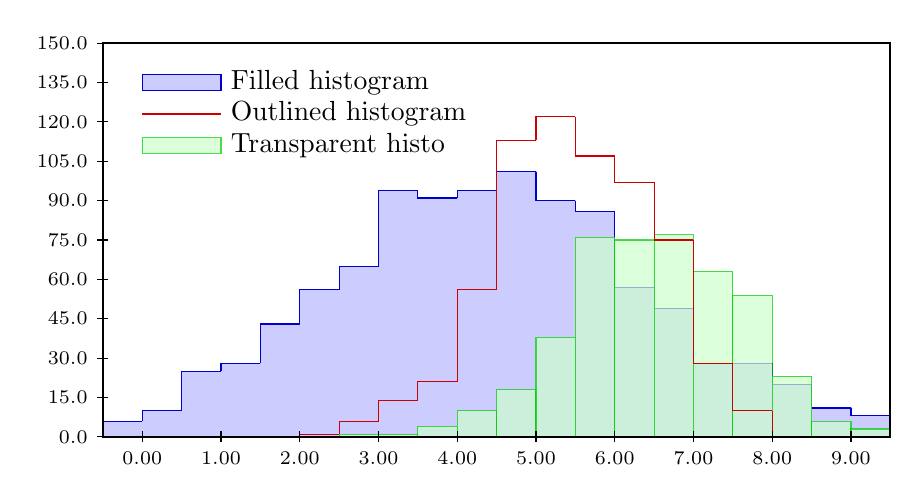
\begin{tikzpicture}
\begin{scope}[]
\clip (0,0) rectangle (10,5);
\begin{scope}[draw=blue!20,fill=blue!20]
\filldraw[] (0.0,0.0) -- (0.0,0.2) -- (0.5,0.2) -- (0.5,0.0);
\filldraw[] (0.5,0.0) -- (0.5,0.33333334) -- (1.0,0.33333334) -- (1.0,0.0);
\filldraw[] (1.0,0.0) -- (1.0,0.8333333) -- (1.5,0.8333333) -- (1.5,0.0);
\filldraw[] (1.5,0.0) -- (1.5,0.93333334) -- (2.0,0.93333334) -- (2.0,0.0);
\filldraw[] (2.0,0.0) -- (2.0,1.4333333) -- (2.5,1.4333333) -- (2.5,0.0);
\filldraw[] (2.5,0.0) -- (2.5,1.8666667) -- (3.0,1.8666667) -- (3.0,0.0);
\filldraw[] (3.0,0.0) -- (3.0,2.1666667) -- (3.5,2.1666667) -- (3.5,0.0);
\filldraw[] (3.5,0.0) -- (3.5,3.1333334) -- (4.0,3.1333334) -- (4.0,0.0);
\filldraw[] (4.0,0.0) -- (4.0,3.0333333) -- (4.5,3.0333333) -- (4.5,0.0);
\filldraw[] (4.5,0.0) -- (4.5,3.1333334) -- (5.0,3.1333334) -- (5.0,0.0);
\filldraw[] (5.0,0.0) -- (5.0,3.3666666) -- (5.5,3.3666666) -- (5.5,0.0);
\filldraw[] (5.5,0.0) -- (5.5,3.0) -- (6.0,3.0) -- (6.0,0.0);
\filldraw[] (6.0,0.0) -- (6.0,2.8666666) -- (6.5,2.8666666) -- (6.5,0.0);
\filldraw[] (6.5,0.0) -- (6.5,1.9) -- (7.0,1.9) -- (7.0,0.0);
\filldraw[] (7.0,0.0) -- (7.0,1.6333333) -- (7.5,1.6333333) -- (7.5,0.0);
\filldraw[] (7.5,0.0) -- (7.5,0.93333334) -- (8.0,0.93333334) -- (8.0,0.0);
\filldraw[] (8.0,0.0) -- (8.0,0.93333334) -- (8.5,0.93333334) -- (8.5,0.0);
\filldraw[] (8.5,0.0) -- (8.5,0.6666667) -- (9.0,0.6666667) -- (9.0,0.0);
\filldraw[] (9.0,0.0) -- (9.0,0.36666667) -- (9.5,0.36666667) -- (9.5,0.0);
\filldraw[] (9.5,0.0) -- (9.5,0.26666668) -- (10.0,0.26666668) -- (10.0,0.0);
\end{scope}
\begin{scope}[blue!80!black]
\draw[] (0.0,0.2) -- (0.5,0.2);
\draw (0.5,0.2) -- (0.5,0.33333334) -- (1.0,0.33333334);
\draw (1.0,0.33333334) -- (1.0,0.8333333) -- (1.5,0.8333333);
\draw (1.5,0.8333333) -- (1.5,0.93333334) -- (2.0,0.93333334);
\draw (2.0,0.93333334) -- (2.0,1.4333333) -- (2.5,1.4333333);
\draw (2.5,1.4333333) -- (2.5,1.8666667) -- (3.0,1.8666667);
\draw (3.0,1.8666667) -- (3.0,2.1666667) -- (3.5,2.1666667);
\draw (3.5,2.1666667) -- (3.5,3.1333334) -- (4.0,3.1333334);
\draw (4.0,3.1333334) -- (4.0,3.0333333) -- (4.5,3.0333333);
\draw (4.5,3.0333333) -- (4.5,3.1333334) -- (5.0,3.1333334);
\draw (5.0,3.1333334) -- (5.0,3.3666666) -- (5.5,3.3666666);
\draw (5.5,3.3666666) -- (5.5,3.0) -- (6.0,3.0);
\draw (6.0,3.0) -- (6.0,2.8666666) -- (6.5,2.8666666);
\draw (6.5,2.8666666) -- (6.5,1.9) -- (7.0,1.9);
\draw (7.0,1.9) -- (7.0,1.6333333) -- (7.5,1.6333333);
\draw (7.5,1.6333333) -- (7.5,0.93333334) -- (8.0,0.93333334);
\draw (8.0,0.93333334) -- (8.0,0.93333334) -- (8.5,0.93333334);
\draw (8.5,0.93333334) -- (8.5,0.6666667) -- (9.0,0.6666667);
\draw (9.0,0.6666667) -- (9.0,0.36666667) -- (9.5,0.36666667);
\draw (9.5,0.36666667) -- (9.5,0.26666668) -- (10.0,0.26666668);
\end{scope}
\begin{scope}[opacity=0.7,draw=green!80!black,fill=green!20]
\filldraw[] (0.0,0.0) -- (0.0,0.0) -- (0.5,0.0) -- (0.5,0.0);
\filldraw[] (0.5,0.0) -- (0.5,0.0) -- (1.0,0.0) -- (1.0,0.0);
\filldraw[] (1.0,0.0) -- (1.0,0.0) -- (1.5,0.0) -- (1.5,0.0);
\filldraw[] (1.5,0.0) -- (1.5,0.0) -- (2.0,0.0) -- (2.0,0.0);
\filldraw[] (2.0,0.0) -- (2.0,0.0) -- (2.5,0.0) -- (2.5,0.0);
\filldraw[] (2.5,0.0) -- (2.5,0.0) -- (3.0,0.0) -- (3.0,0.0);
\filldraw[] (3.0,0.0) -- (3.0,0.033333335) -- (3.5,0.033333335) -- (3.5,0.0);
\filldraw[] (3.5,0.0) -- (3.5,0.033333335) -- (4.0,0.033333335) -- (4.0,0.0);
\filldraw[] (4.0,0.0) -- (4.0,0.13333334) -- (4.5,0.13333334) -- (4.5,0.0);
\filldraw[] (4.5,0.0) -- (4.5,0.33333334) -- (5.0,0.33333334) -- (5.0,0.0);
\filldraw[] (5.0,0.0) -- (5.0,0.6) -- (5.5,0.6) -- (5.5,0.0);
\filldraw[] (5.5,0.0) -- (5.5,1.2666667) -- (6.0,1.2666667) -- (6.0,0.0);
\filldraw[] (6.0,0.0) -- (6.0,2.5333333) -- (6.5,2.5333333) -- (6.5,0.0);
\filldraw[] (6.5,0.0) -- (6.5,2.5) -- (7.0,2.5) -- (7.0,0.0);
\filldraw[] (7.0,0.0) -- (7.0,2.5666666) -- (7.5,2.5666666) -- (7.5,0.0);
\filldraw[] (7.5,0.0) -- (7.5,2.1) -- (8.0,2.1) -- (8.0,0.0);
\filldraw[] (8.0,0.0) -- (8.0,1.8) -- (8.5,1.8) -- (8.5,0.0);
\filldraw[] (8.5,0.0) -- (8.5,0.76666665) -- (9.0,0.76666665) -- (9.0,0.0);
\filldraw[] (9.0,0.0) -- (9.0,0.2) -- (9.5,0.2) -- (9.5,0.0);
\filldraw[] (9.5,0.0) -- (9.5,0.1) -- (10.0,0.1) -- (10.0,0.0);
\end{scope}
\begin{scope}[red!80!black]
\draw[] (0.0,0.0) -- (0.5,0.0);
\draw (0.5,0.0) -- (0.5,0.0) -- (1.0,0.0);
\draw (1.0,0.0) -- (1.0,0.0) -- (1.5,0.0);
\draw (1.5,0.0) -- (1.5,0.0) -- (2.0,0.0);
\draw (2.0,0.0) -- (2.0,0.0) -- (2.5,0.0);
\draw (2.5,0.0) -- (2.5,0.033333335) -- (3.0,0.033333335);
\draw (3.0,0.033333335) -- (3.0,0.2) -- (3.5,0.2);
\draw (3.5,0.2) -- (3.5,0.46666667) -- (4.0,0.46666667);
\draw (4.0,0.46666667) -- (4.0,0.7) -- (4.5,0.7);
\draw (4.5,0.7) -- (4.5,1.8666667) -- (5.0,1.8666667);
\draw (5.0,1.8666667) -- (5.0,3.7666667) -- (5.5,3.7666667);
\draw (5.5,3.7666667) -- (5.5,4.0666666) -- (6.0,4.0666666);
\draw (6.0,4.0666666) -- (6.0,3.5666666) -- (6.5,3.5666666);
\draw (6.5,3.5666666) -- (6.5,3.2333333) -- (7.0,3.2333333);
\draw (7.0,3.2333333) -- (7.0,2.5) -- (7.5,2.5);
\draw (7.5,2.5) -- (7.5,0.93333334) -- (8.0,0.93333334);
\draw (8.0,0.93333334) -- (8.0,0.33333334) -- (8.5,0.33333334);
\draw (8.5,0.33333334) -- (8.5,0.0) -- (9.0,0.0);
\draw (9.0,0.0) -- (9.0,0.0) -- (9.5,0.0);
\draw (9.5,0.0) -- (9.5,0.0) -- (10.0,0.0);
\end{scope}
\end{scope}
\draw (0.5,0cm + 2pt) -- (0.5, 0cm -2pt) node[below] {\scriptsize{\num[round-mode=places,round-precision=2]{0}}};
\draw (1.5,0cm + 2pt) -- (1.5, 0cm -2pt) node[below] {\scriptsize{\num[round-mode=places,round-precision=2]{1}}};
\draw (2.5,0cm + 2pt) -- (2.5, 0cm -2pt) node[below] {\scriptsize{\num[round-mode=places,round-precision=2]{2}}};
\draw (3.5,0cm + 2pt) -- (3.5, 0cm -2pt) node[below] {\scriptsize{\num[round-mode=places,round-precision=2]{3}}};
\draw (4.5,0cm + 2pt) -- (4.5, 0cm -2pt) node[below] {\scriptsize{\num[round-mode=places,round-precision=2]{4}}};
\draw (5.5,0cm + 2pt) -- (5.5, 0cm -2pt) node[below] {\scriptsize{\num[round-mode=places,round-precision=2]{5}}};
\draw (6.5,0cm + 2pt) -- (6.5, 0cm -2pt) node[below] {\scriptsize{\num[round-mode=places,round-precision=2]{6}}};
\draw (7.5,0cm + 2pt) -- (7.5, 0cm -2pt) node[below] {\scriptsize{\num[round-mode=places,round-precision=2]{7}}};
\draw (8.5,0cm + 2pt) -- (8.5, 0cm -2pt) node[below] {\scriptsize{\num[round-mode=places,round-precision=2]{8}}};
\draw (9.5,0cm + 2pt) -- (9.5, 0cm -2pt) node[below] {\scriptsize{\num[round-mode=places,round-precision=2]{9}}};
\draw (0cm + 2pt,0.    ) -- (0cm-2pt,0.    ) node[left] {\scriptsize{\num[round-mode=places,round-precision=1]{0}}};
\draw (0cm + 2pt,0.5    ) -- (0cm-2pt,0.5    ) node[left] {\scriptsize{\num[round-mode=places,round-precision=1]{15}}};
\draw (0cm + 2pt,1.    ) -- (0cm-2pt,1.    ) node[left] {\scriptsize{\num[round-mode=places,round-precision=1]{30}}};
\draw (0cm + 2pt,1.5    ) -- (0cm-2pt,1.5    ) node[left] {\scriptsize{\num[round-mode=places,round-precision=1]{45}}};
\draw (0cm + 2pt,2.    ) -- (0cm-2pt,2.    ) node[left] {\scriptsize{\num[round-mode=places,round-precision=1]{60}}};
\draw (0cm + 2pt,2.5    ) -- (0cm-2pt,2.5    ) node[left] {\scriptsize{\num[round-mode=places,round-precision=1]{75}}};
\draw (0cm + 2pt,3.    ) -- (0cm-2pt,3.    ) node[left] {\scriptsize{\num[round-mode=places,round-precision=1]{90}}};
\draw (0cm + 2pt,3.5    ) -- (0cm-2pt,3.5    ) node[left] {\scriptsize{\num[round-mode=places,round-precision=1]{105}}};
\draw (0cm + 2pt,4.    ) -- (0cm-2pt,4.    ) node[left] {\scriptsize{\num[round-mode=places,round-precision=1]{120}}};
\draw (0cm + 2pt,4.5    ) -- (0cm-2pt,4.5    ) node[left] {\scriptsize{\num[round-mode=places,round-precision=1]{135}}};
\draw (0cm + 2pt,5.    ) -- (0cm-2pt,5.    ) node[left] {\scriptsize{\num[round-mode=places,round-precision=1]{150}}};
\draw[thick] (0,0) rectangle (10,5);
\draw[draw=blue!20,fill=blue!20] (0.5,4.4) rectangle (1.5,4.6);
\draw[blue!80!black] (0.5,4.4) rectangle (1.5,4.6);
\node[right,] at (1.5,4.5) {Filled histogram};
\draw[red!80!black] (0.5,4.1) -- (1.5,4.1);
\node[right,] at (1.5,4.1) {Outlined histogram};
\draw[opacity=0.7,draw=green!80!black,fill=green!20] (0.5,3.6000001) rectangle (1.5,3.8);
\node[right,] at (1.5,3.7) {Transparent histo};
\end{tikzpicture}
%%% Local Variables: 
%%% mode: latex 
%%% TeX-master: "master" 
%%% End:


  \caption{Three histograms in the same figure}
\end{figure}

\begin{figure}[H]
  \centering
  \documentclass{standalone}
\ifx\HCode\UnDef\else\def\pgfsysdriver{pgfsys-tex4ht.def}\fi
\usepackage[usenames,dvipsnames,svgnames,table]{xcolor}
\usepackage{tikz}
\usepackage{color}
\usepackage{siunitx}
\usetikzlibrary{arrows,shapes}
\begin{document}
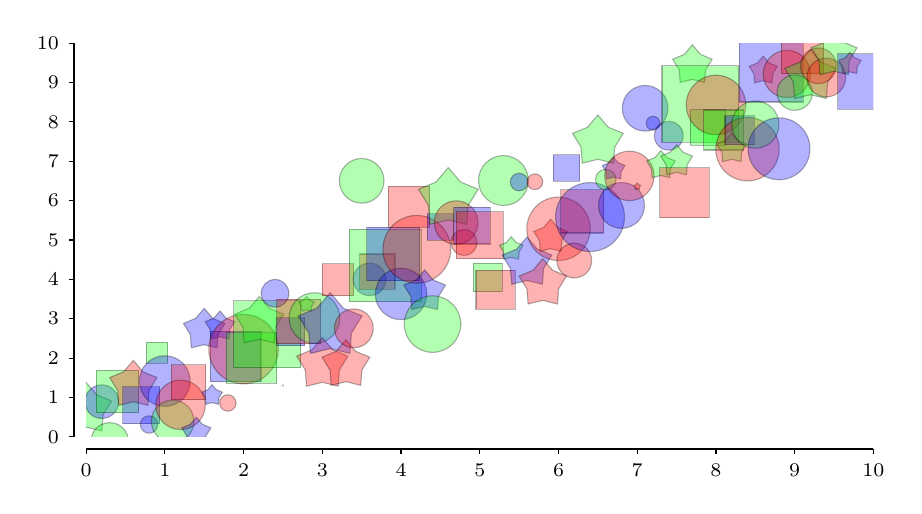
\begin{tikzpicture}
\begin{scope}[]
\pgfpointadd{\pgfpointxy {0.0} {0.0}} {\pgfpoint{0cm}{0cm}}\pgfpathmoveto{ NIL }
\pgfpointadd{\pgfpointxy {0.0} {0.0}} {\pgfpoint{10cm}{0cm}}\pgfpathlineto{ NIL }
\pgfpointadd{\pgfpointxy {0.0} {0.0}} {\pgfpoint{10cm}{5cm}}\pgfpathlineto{ NIL }
\pgfpointadd{\pgfpointxy {0.0} {0.0}} {\pgfpoint{0cm}{5cm}}\pgfpathlineto{ NIL }
\pgfpathclose
\pgfusepath{  clip, }
\begin{scope}[shift={(0.0,0.0)}]
\pgfsetxvec{\pgfpoint{1.0cm}{0cm}}
\pgfsetyvec{\pgfpoint{0cm}{0.5cm}}
\begin{scope}[shift={(0.0,0.0)}]
\node at (0.0,0.7006110756122909) [draw=black,fill=green,opacity=0.3,star,inner sep=0.0mm,minimum width =6.800587496850904mm,minimum height=6.800587496850904mm] {};
\node at (0.1,-0.7734106387051958) [draw=black,fill=green,opacity=0.3,star,inner sep=0.0mm,minimum width =3.6460143198852952mm,minimum height=3.6460143198852952mm] {};
\node at (0.2,0.8936623412927944) [draw=black,fill=blue,opacity=0.3,circle,inner sep=0.0mm,minimum width =4.272260443846609mm,minimum height=4.272260443846609mm] {};
\node at (0.3,-0.11494552503266542) [draw=black,fill=green,opacity=0.3,circle,inner sep=0.0mm,minimum width =4.752905216170019mm,minimum height=4.752905216170019mm] {};
\node at (0.4,1.150349541366745) [draw=black,fill=green,opacity=0.3,rectangle,inner sep=0.0mm,minimum width =5.378692570370324mm,minimum height=5.378692570370324mm] {};
\node at (0.5,-1.8588294510295857) [draw=black,fill=red,opacity=0.3,circle,inner sep=0.0mm,minimum width =5.952965504524424mm,minimum height=5.952965504524424mm] {};
\node at (0.6,1.3106837531472841) [draw=black,fill=red,opacity=0.3,star,inner sep=0.0mm,minimum width =6.315038332090647mm,minimum height=6.315038332090647mm] {};
\node at (0.7,0.8044580736841929) [draw=black,fill=blue,opacity=0.3,rectangle,inner sep=0.0mm,minimum width =4.731654041668135mm,minimum height=4.731654041668135mm] {};
\node at (0.8,0.31356219753880626) [draw=black,fill=blue,opacity=0.3,circle,inner sep=0.0mm,minimum width =2.220868006425221mm,minimum height=2.220868006425221mm] {};
\node at (0.90000004,2.1329623554392843) [draw=black,fill=green,opacity=0.3,rectangle,inner sep=0.0mm,minimum width =2.6819606796927187mm,minimum height=2.6819606796927187mm] {};
\node at (1.0,1.4159074987429303) [draw=black,fill=blue,opacity=0.3,circle,inner sep=0.0mm,minimum width =6.442954524709304mm,minimum height=6.442954524709304mm] {};
\node at (1.1,0.39295316234538624) [draw=black,fill=green,opacity=0.3,circle,inner sep=0.0mm,minimum width =5.399756727494323mm,minimum height=5.399756727494323mm] {};
\node at (1.2,0.8132344213873199) [draw=black,fill=red,opacity=0.3,circle,inner sep=0.0mm,minimum width =6.287295603642487mm,minimum height=6.287295603642487mm] {};
\node at (1.3000001,1.3872414968679347) [draw=black,fill=red,opacity=0.3,rectangle,inner sep=0.0mm,minimum width =4.409969468970658mm,minimum height=4.409969468970658mm] {};
\node at (1.4,0.1090123422278444) [draw=black,fill=blue,opacity=0.3,star,inner sep=0.0mm,minimum width =3.890683836470598mm,minimum height=3.890683836470598mm] {};
\node at (1.5,2.709103305949749) [draw=black,fill=blue,opacity=0.3,star,inner sep=0.0mm,minimum width =5.542198749418023mm,minimum height=5.542198749418023mm] {};
\node at (1.6,1.0500102467760244) [draw=black,fill=blue,opacity=0.3,star,inner sep=0.0mm,minimum width =2.741419975172315mm,minimum height=2.741419975172315mm] {};
\node at (1.7,2.804268401979424) [draw=black,fill=blue,opacity=0.3,star,inner sep=0.0mm,minimum width =3.9322501146273385mm,minimum height=3.9322501146273385mm] {};
\node at (1.8000001,0.8604649480672137) [draw=black,fill=red,opacity=0.3,circle,inner sep=0.0mm,minimum width =2.090570155891645mm,minimum height=2.090570155891645mm] {};
\node at (1.9,2.0407167342406702) [draw=black,fill=blue,opacity=0.3,rectangle,inner sep=0.0mm,minimum width =6.435583612838957mm,minimum height=6.435583612838957mm] {};
\node at (2.0,2.2286922355247976) [draw=black,fill=red,opacity=0.3,circle,inner sep=0.0mm,minimum width =8.832062398405533mm,minimum height=8.832062398405533mm] {};
\node at (2.1000001,2.000614315353244) [draw=black,fill=green,opacity=0.3,rectangle,inner sep=0.0mm,minimum width =6.388258996727354mm,minimum height=6.388258996727354mm] {};
\node at (2.2,2.9135575687932036) [draw=black,fill=green,opacity=0.3,star,inner sep=0.0mm,minimum width =6.503302028106489mm,minimum height=6.503302028106489mm] {};
\node at (2.3,2.6057336498405617) [draw=black,fill=green,opacity=0.3,rectangle,inner sep=0.0mm,minimum width =8.532957621356363mm,minimum height=8.532957621356363mm] {};
\node at (2.4,3.644968288436833) [draw=black,fill=blue,opacity=0.3,circle,inner sep=0.0mm,minimum width =3.5184462877320484mm,minimum height=3.5184462877320484mm] {};
\node at (2.5,1.3041485524642158) [draw=black,fill=red,opacity=0.3,star,inner sep=0.0mm,minimum width =0.1mm,minimum height=0.1mm] {};
\node at (2.6000001,2.667533754247742) [draw=black,fill=blue,opacity=0.3,rectangle,inner sep=0.0mm,minimum width =3.570086353410753mm,minimum height=3.570086353410753mm] {};
\node at (2.7,2.931016904802913) [draw=black,fill=red,opacity=0.3,rectangle,inner sep=0.0mm,minimum width =5.6091544426281805mm,minimum height=5.6091544426281805mm] {};
\node at (2.8,3.3603908893740035) [draw=black,fill=green,opacity=0.3,star,inner sep=0.0mm,minimum width =2.0136506057312813mm,minimum height=2.0136506057312813mm] {};
\node at (2.9,3.0166066169551957) [draw=black,fill=green,opacity=0.3,circle,inner sep=0.0mm,minimum width =6.4448519208068795mm,minimum height=6.4448519208068795mm] {};
\node at (3.0,1.8390865566362826) [draw=black,fill=red,opacity=0.3,star,inner sep=0.0mm,minimum width =6.829311725505772mm,minimum height=6.829311725505772mm] {};
\node at (3.1000001,2.8090410129452135) [draw=black,fill=blue,opacity=0.3,star,inner sep=0.0mm,minimum width =8.526654123325148mm,minimum height=8.526654123325148mm] {};
\node at (3.2,3.9904474878671072) [draw=black,fill=red,opacity=0.3,rectangle,inner sep=0.0mm,minimum width =4.028381917972839mm,minimum height=4.028381917972839mm] {};
\node at (3.3,1.826071884695202) [draw=black,fill=red,opacity=0.3,star,inner sep=0.0mm,minimum width =6.384264845787511mm,minimum height=6.384264845787511mm] {};
\node at (3.4,2.756052548182273) [draw=black,fill=red,opacity=0.3,circle,inner sep=0.0mm,minimum width =4.926370312479602mm,minimum height=4.926370312479602mm] {};
\node at (3.5,6.5025300185625525) [draw=black,fill=green,opacity=0.3,circle,inner sep=0.0mm,minimum width =5.666485070612519mm,minimum height=5.666485070612519mm] {};
\node at (3.6000001,4.001097507639919) [draw=black,fill=blue,opacity=0.3,circle,inner sep=0.0mm,minimum width =4.138853579394104mm,minimum height=4.138853579394104mm] {};
\node at (3.7,4.19701461175223) [draw=black,fill=red,opacity=0.3,rectangle,inner sep=0.0mm,minimum width =4.472865794162527mm,minimum height=4.472865794162527mm] {};
\node at (3.8,4.350897011030634) [draw=black,fill=green,opacity=0.3,rectangle,inner sep=0.0mm,minimum width =9.158076511100287mm,minimum height=9.158076511100287mm] {};
\node at (3.9,4.642078870376014) [draw=black,fill=blue,opacity=0.3,rectangle,inner sep=0.0mm,minimum width =6.753169795357893mm,minimum height=6.753169795357893mm] {};
\node at (4.0,3.6289117627006258) [draw=black,fill=blue,opacity=0.3,circle,inner sep=0.0mm,minimum width =6.534480556075062mm,minimum height=6.534480556075062mm] {};
\node at (4.1,5.845577054396422) [draw=black,fill=red,opacity=0.3,rectangle,inner sep=0.0mm,minimum width =5.228700941694266mm,minimum height=5.228700941694266mm] {};
\node at (4.2000003,4.761594535940161) [draw=black,fill=red,opacity=0.3,circle,inner sep=0.0mm,minimum width =8.616717667652617mm,minimum height=8.616717667652617mm] {};
\node at (4.3,3.6832125800853603) [draw=black,fill=blue,opacity=0.3,star,inner sep=0.0mm,minimum width =5.5685232481589555mm,minimum height=5.5685232481589555mm] {};
\node at (4.4,2.864283362376743) [draw=black,fill=green,opacity=0.3,circle,inner sep=0.0mm,minimum width =7.180178548504459mm,minimum height=7.180178548504459mm] {};
\node at (4.5,5.33093581499132) [draw=black,fill=blue,opacity=0.3,rectangle,inner sep=0.0mm,minimum width =3.3469949020565597mm,minimum height=3.3469949020565597mm] {};
\node at (4.6,6.041421616562869) [draw=black,fill=green,opacity=0.3,star,inner sep=0.0mm,minimum width =7.966304756185466mm,minimum height=7.966304756185466mm] {};
\node at (4.7000003,5.442247437396192) [draw=black,fill=red,opacity=0.3,circle,inner sep=0.0mm,minimum width =5.544290891592568mm,minimum height=5.544290891592568mm] {};
\node at (4.8,4.93606313648638) [draw=black,fill=red,opacity=0.3,circle,inner sep=0.0mm,minimum width =3.299993379153297mm,minimum height=3.299993379153297mm] {};
\node at (4.9,5.363716700207102) [draw=black,fill=blue,opacity=0.3,rectangle,inner sep=0.0mm,minimum width =4.668878509443525mm,minimum height=4.668878509443525mm] {};
\node at (5.0,5.122315577086894) [draw=black,fill=red,opacity=0.3,rectangle,inner sep=0.0mm,minimum width =5.995732392446039mm,minimum height=5.995732392446039mm] {};
\node at (5.1,4.047857456792124) [draw=black,fill=green,opacity=0.3,rectangle,inner sep=0.0mm,minimum width =3.657374369389488mm,minimum height=3.657374369389488mm] {};
\node at (5.2000003,3.7346048874961344) [draw=black,fill=red,opacity=0.3,rectangle,inner sep=0.0mm,minimum width =4.962970149068191mm,minimum height=4.962970149068191mm] {};
\node at (5.3,6.509910638266652) [draw=black,fill=green,opacity=0.3,circle,inner sep=0.0mm,minimum width =6.333681610089098mm,minimum height=6.333681610089098mm] {};
\node at (5.4,4.768558276733036) [draw=black,fill=green,opacity=0.3,star,inner sep=0.0mm,minimum width =3.139338973267701mm,minimum height=3.139338973267701mm] {};
\node at (5.5,6.471632805052075) [draw=black,fill=blue,opacity=0.3,circle,inner sep=0.0mm,minimum width =2.242487981845843mm,minimum height=2.242487981845843mm] {};
\node at (5.6,4.412349829576712) [draw=black,fill=blue,opacity=0.3,star,inner sep=0.0mm,minimum width =6.636871505233696mm,minimum height=6.636871505233696mm] {};
\node at (5.7000003,6.4782834007708) [draw=black,fill=red,opacity=0.3,circle,inner sep=0.0mm,minimum width =1.997719382164059mm,minimum height=1.997719382164059mm] {};
\node at (5.8,3.888256448685543) [draw=black,fill=red,opacity=0.3,star,inner sep=0.0mm,minimum width =6.343367365490759mm,minimum height=6.343367365490759mm] {};
\node at (5.9,5.078279802998635) [draw=black,fill=red,opacity=0.3,star,inner sep=0.0mm,minimum width =4.490472975152459mm,minimum height=4.490472975152459mm] {};
\node at (6.0,5.284365368010424) [draw=black,fill=red,opacity=0.3,circle,inner sep=0.0mm,minimum width =8.054282226642933mm,minimum height=8.054282226642933mm] {};
\node at (6.1,6.829763820733274) [draw=black,fill=blue,opacity=0.3,rectangle,inner sep=0.0mm,minimum width =3.3619194777359462mm,minimum height=3.3619194777359462mm] {};
\node at (6.2000003,4.477859423057665) [draw=black,fill=red,opacity=0.3,circle,inner sep=0.0mm,minimum width =4.416702285833479mm,minimum height=4.416702285833479mm] {};
\node at (6.3,5.724072343679785) [draw=black,fill=red,opacity=0.3,rectangle,inner sep=0.0mm,minimum width =5.479225546205502mm,minimum height=5.479225546205502mm] {};
\node at (6.4,5.582183907466308) [draw=black,fill=blue,opacity=0.3,circle,inner sep=0.0mm,minimum width =8.755484725321633mm,minimum height=8.755484725321633mm] {};
\node at (6.5,7.4982281143890805) [draw=black,fill=green,opacity=0.3,star,inner sep=0.0mm,minimum width =6.752916955966518mm,minimum height=6.752916955966518mm] {};
\node at (6.6,6.5356869753944915) [draw=black,fill=green,opacity=0.3,circle,inner sep=0.0mm,minimum width =2.606092005077641mm,minimum height=2.606092005077641mm] {};
\node at (6.7000003,6.797514749450102) [draw=black,fill=blue,opacity=0.3,star,inner sep=0.0mm,minimum width =3.02969016773718mm,minimum height=3.02969016773718mm] {};
\node at (6.8,5.878321174990502) [draw=black,fill=blue,opacity=0.3,circle,inner sep=0.0mm,minimum width =5.828193229435527mm,minimum height=5.828193229435527mm] {};
\node at (6.9,6.628377924035324) [draw=black,fill=red,opacity=0.3,circle,inner sep=0.0mm,minimum width =6.2854079830836325mm,minimum height=6.2854079830836325mm] {};
\node at (7.0,6.3573012886568945) [draw=black,fill=red,opacity=0.3,star,inner sep=0.0mm,minimum width =0.8690510961575137mm,minimum height=0.8690510961575137mm] {};
\node at (7.1,8.345404789338616) [draw=black,fill=blue,opacity=0.3,circle,inner sep=0.0mm,minimum width =5.8006348111687345mm,minimum height=5.8006348111687345mm] {};
\node at (7.2000003,7.967598147295394) [draw=black,fill=blue,opacity=0.3,circle,inner sep=0.0mm,minimum width =1.7436408842924331mm,minimum height=1.7436408842924331mm] {};
\node at (7.3,6.891026655893629) [draw=black,fill=green,opacity=0.3,star,inner sep=0.0mm,minimum width =3.7922490480733426mm,minimum height=3.7922490480733426mm] {};
\node at (7.4,7.6482099490320286) [draw=black,fill=blue,opacity=0.3,circle,inner sep=0.0mm,minimum width =3.656084501913735mm,minimum height=3.656084501913735mm] {};
\node at (7.5,6.999254458639783) [draw=black,fill=green,opacity=0.3,star,inner sep=0.0mm,minimum width =4.224003221948369mm,minimum height=4.224003221948369mm] {};
\node at (7.6,6.196770940314023) [draw=black,fill=red,opacity=0.3,rectangle,inner sep=0.0mm,minimum width =6.3428711314490265mm,minimum height=6.3428711314490265mm] {};
\node at (7.7000003,9.428989133340579) [draw=black,fill=green,opacity=0.3,star,inner sep=0.0mm,minimum width =5.260159680830009mm,minimum height=5.260159680830009mm] {};
\node at (7.8,8.453571476123223) [draw=black,fill=green,opacity=0.3,rectangle,inner sep=0.0mm,minimum width =9.712893227331783mm,minimum height=9.712893227331783mm] {};
\node at (7.9,7.852220709777919) [draw=black,fill=green,opacity=0.3,rectangle,inner sep=0.0mm,minimum width =4.517086585502086mm,minimum height=4.517086585502086mm] {};
\node at (8.0,8.430187892265131) [draw=black,fill=red,opacity=0.3,circle,inner sep=0.0mm,minimum width =7.555025786576515mm,minimum height=7.555025786576515mm] {};
\node at (8.1,7.793044975322582) [draw=black,fill=green,opacity=0.3,rectangle,inner sep=0.0mm,minimum width =5.079797169365946mm,minimum height=5.079797169365946mm] {};
\node at (8.2,7.312282164316225) [draw=black,fill=green,opacity=0.3,star,inner sep=0.0mm,minimum width =3.967699049445409mm,minimum height=3.967699049445409mm] {};
\node at (8.3,7.787710828673871) [draw=black,fill=blue,opacity=0.3,rectangle,inner sep=0.0mm,minimum width =3.719869417804288mm,minimum height=3.719869417804288mm] {};
\node at (8.400001,7.306777225169212) [draw=black,fill=red,opacity=0.3,circle,inner sep=0.0mm,minimum width =8.057531066025984mm,minimum height=8.057531066025984mm] {};
\node at (8.5,7.9298590184799975) [draw=black,fill=green,opacity=0.3,circle,inner sep=0.0mm,minimum width =5.9944200154766385mm,minimum height=5.9944200154766385mm] {};
\node at (8.6,9.295232642920105) [draw=black,fill=red,opacity=0.3,star,inner sep=0.0mm,minimum width =3.743927705858683mm,minimum height=3.743927705858683mm] {};
\node at (8.7,9.318646914421347) [draw=black,fill=blue,opacity=0.3,rectangle,inner sep=0.0mm,minimum width =8.138066340772387mm,minimum height=8.138066340772387mm] {};
\node at (8.8,7.316350266830897) [draw=black,fill=blue,opacity=0.3,circle,inner sep=0.0mm,minimum width =7.86319292065604mm,minimum height=7.86319292065604mm] {};
\node at (8.900001,9.216994207193585) [draw=black,fill=red,opacity=0.3,circle,inner sep=0.0mm,minimum width =5.99600368059251mm,minimum height=5.99600368059251mm] {};
\node at (9.0,8.74333360842608) [draw=black,fill=green,opacity=0.3,circle,inner sep=0.0mm,minimum width =4.494589002237348mm,minimum height=4.494589002237348mm] {};
\node at (9.1,9.76380195703883) [draw=black,fill=red,opacity=0.3,rectangle,inner sep=0.0mm,minimum width =5.397227907992171mm,minimum height=5.397227907992171mm] {};
\node at (9.2,9.14773387995154) [draw=black,fill=green,opacity=0.3,star,inner sep=0.0mm,minimum width =6.843927451359315mm,minimum height=6.843927451359315mm] {};
\node at (9.3,9.424299393498773) [draw=black,fill=red,opacity=0.3,circle,inner sep=0.0mm,minimum width =4.535659005201774mm,minimum height=4.535659005201774mm] {};
\node at (9.400001,9.126131720465992) [draw=black,fill=red,opacity=0.3,circle,inner sep=0.0mm,minimum width =4.923542124874365mm,minimum height=4.923542124874365mm] {};
\node at (9.5,9.692677643957623) [draw=black,fill=green,opacity=0.3,star,inner sep=0.0mm,minimum width =6.112567248997191mm,minimum height=6.112567248997191mm] {};
\node at (9.6,10.387040958723833) [draw=black,fill=red,opacity=0.3,circle,inner sep=0.0mm,minimum width =3.7592783093430375mm,minimum height=3.7592783093430375mm] {};
\node at (9.7,9.468552761972866) [draw=black,fill=red,opacity=0.3,star,inner sep=0.0mm,minimum width =2.9689778407290563mm,minimum height=2.9689778407290563mm] {};
\node at (9.8,10.626789262788723) [draw=black,fill=red,opacity=0.3,circle,inner sep=0.0mm,minimum width =0.9339116799269327mm,minimum height=0.9339116799269327mm] {};
\node at (9.900001,9.024151475469719) [draw=black,fill=blue,opacity=0.3,rectangle,inner sep=0.0mm,minimum width =7.0706247041934445mm,minimum height=7.0706247041934445mm] {};
\end{scope}
\pgfsetxvec{\pgfpoint{1cm}{0cm}}
\pgfsetyvec{\pgfpoint{0cm}{1cm}}
\end{scope}
\end{scope}
\begin{scope}[shift={(0.0,0.0)}]
\pgfsetxvec{\pgfpoint{1.0cm}{0cm}}
\pgfsetyvec{\pgfpoint{0cm}{0.5cm}}
\begin{scope}[shift={(0.0,0.0)}]
\begin{scope}[thick,black,fill=white]
\pgfpointadd{\pgfpointxy {0.0} {0.0}} {\pgfpoint{0}{-0.15cm}}\pgfpathmoveto{ NIL }
\pgfpointadd{\pgfpointxy {10.0} {0.0}} {\pgfpoint{0}{-0.15cm}}\pgfpathlineto{ NIL }
\pgfpointadd{\pgfpointxy {0.0} {0.0}} {\pgfpoint{-0.15cm}{0}}\pgfpathmoveto{ NIL }
\pgfpointadd{\pgfpointxy {0.0} {10.0}} {\pgfpoint{-0.15cm}{0}}\pgfpathlineto{ NIL }
\pgfusepath{ stroke, }
\end{scope}
\begin{scope}[yshift=-0.15cm]
\draw[] [shift={(0.0,0.0)}] (0,0) -- (0,-2pt) node[below]{ \scriptsize{\num[round-mode=places,round-precision=0]{0}}};
\draw[] [shift={(1.0,0.0)}] (0,0) -- (0,-2pt) node[below]{ \scriptsize{\num[round-mode=places,round-precision=0]{1}}};
\draw[] [shift={(2.0,0.0)}] (0,0) -- (0,-2pt) node[below]{ \scriptsize{\num[round-mode=places,round-precision=0]{2}}};
\draw[] [shift={(3.0,0.0)}] (0,0) -- (0,-2pt) node[below]{ \scriptsize{\num[round-mode=places,round-precision=0]{3}}};
\draw[] [shift={(4.0,0.0)}] (0,0) -- (0,-2pt) node[below]{ \scriptsize{\num[round-mode=places,round-precision=0]{4}}};
\draw[] [shift={(5.0,0.0)}] (0,0) -- (0,-2pt) node[below]{ \scriptsize{\num[round-mode=places,round-precision=0]{5}}};
\draw[] [shift={(6.0,0.0)}] (0,0) -- (0,-2pt) node[below]{ \scriptsize{\num[round-mode=places,round-precision=0]{6}}};
\draw[] [shift={(7.0,0.0)}] (0,0) -- (0,-2pt) node[below]{ \scriptsize{\num[round-mode=places,round-precision=0]{7}}};
\draw[] [shift={(8.0,0.0)}] (0,0) -- (0,-2pt) node[below]{ \scriptsize{\num[round-mode=places,round-precision=0]{8}}};
\draw[] [shift={(9.0,0.0)}] (0,0) -- (0,-2pt) node[below]{ \scriptsize{\num[round-mode=places,round-precision=0]{9}}};
\draw[] [shift={(10.0,0.0)}] (0,0) -- (0,-2pt) node[below]{ \scriptsize{\num[round-mode=places,round-precision=0]{10}}};
\end{scope}
\begin{scope}[xshift=-0.15cm]
\draw[] [shift={(0.0,0.0)}] (0,0) -- (-2pt,0) node[left]{ \scriptsize{\num[round-mode=places,round-precision=0]{0}}};
\draw[] [shift={(0.0,1.0)}] (0,0) -- (-2pt,0) node[left]{ \scriptsize{\num[round-mode=places,round-precision=0]{1}}};
\draw[] [shift={(0.0,2.0)}] (0,0) -- (-2pt,0) node[left]{ \scriptsize{\num[round-mode=places,round-precision=0]{2}}};
\draw[] [shift={(0.0,3.0)}] (0,0) -- (-2pt,0) node[left]{ \scriptsize{\num[round-mode=places,round-precision=0]{3}}};
\draw[] [shift={(0.0,4.0)}] (0,0) -- (-2pt,0) node[left]{ \scriptsize{\num[round-mode=places,round-precision=0]{4}}};
\draw[] [shift={(0.0,5.0)}] (0,0) -- (-2pt,0) node[left]{ \scriptsize{\num[round-mode=places,round-precision=0]{5}}};
\draw[] [shift={(0.0,6.0)}] (0,0) -- (-2pt,0) node[left]{ \scriptsize{\num[round-mode=places,round-precision=0]{6}}};
\draw[] [shift={(0.0,7.0)}] (0,0) -- (-2pt,0) node[left]{ \scriptsize{\num[round-mode=places,round-precision=0]{7}}};
\draw[] [shift={(0.0,8.0)}] (0,0) -- (-2pt,0) node[left]{ \scriptsize{\num[round-mode=places,round-precision=0]{8}}};
\draw[] [shift={(0.0,9.0)}] (0,0) -- (-2pt,0) node[left]{ \scriptsize{\num[round-mode=places,round-precision=0]{9}}};
\draw[] [shift={(0.0,10.0)}] (0,0) -- (-2pt,0) node[left]{ \scriptsize{\num[round-mode=places,round-precision=0]{10}}};
\end{scope}
\end{scope}
\pgfsetxvec{\pgfpoint{1cm}{0cm}}
\pgfsetyvec{\pgfpoint{0cm}{1cm}}
\end{scope}
\end{tikzpicture}
\end{document}

  \caption{Nodes of different sizes.}
\end{figure}

\begin{figure}[H]
  \centering
  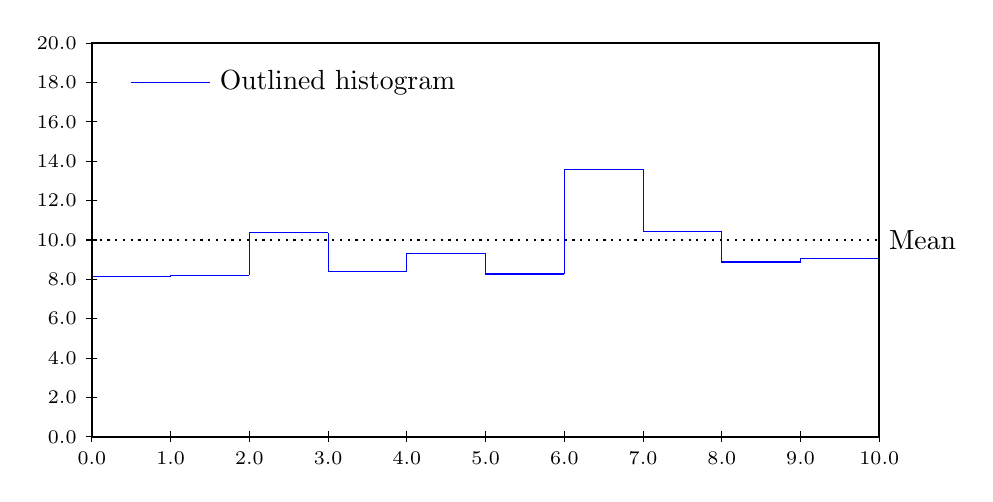
\begin{tikzpicture}
\begin{scope}[]
\clip (0,0) rectangle (10,5);
\begin{scope}[blue]
\draw[] (0.0,2.040753989729346) -- (1.0,2.040753989729346);
\draw (1.0,2.040753989729346) -- (1.0,2.0520371396851527) -- (2.0,2.0520371396851527);
\draw (2.0,2.0520371396851527) -- (2.0,2.589490136587087) -- (3.0,2.589490136587087);
\draw (3.0,2.589490136587087) -- (3.0,2.10531930397396) -- (4.0,2.10531930397396);
\draw (4.0,2.10531930397396) -- (4.0,2.328047479221825) -- (5.0,2.328047479221825);
\draw (5.0,2.328047479221825) -- (5.0,2.067390163042384) -- (6.0,2.067390163042384);
\draw (6.0,2.067390163042384) -- (6.0,3.3961419895360887) -- (7.0,3.3961419895360887);
\draw (7.0,3.3961419895360887) -- (7.0,2.6085288458106475) -- (8.0,2.6085288458106475);
\draw (8.0,2.6085288458106475) -- (8.0,2.2210174657245827) -- (9.0,2.2210174657245827);
\draw (9.0,2.2210174657245827) -- (9.0,2.2670683657782047) -- (10.0,2.2670683657782047);
\end{scope}
\end{scope}
\draw (0,0cm + 2pt) -- (0, 0cm -2pt) node[below] {\scriptsize{\num[round-mode=places,round-precision=1]{0}}};
\draw (1,0cm + 2pt) -- (1, 0cm -2pt) node[below] {\scriptsize{\num[round-mode=places,round-precision=1]{1}}};
\draw (2,0cm + 2pt) -- (2, 0cm -2pt) node[below] {\scriptsize{\num[round-mode=places,round-precision=1]{2}}};
\draw (3,0cm + 2pt) -- (3, 0cm -2pt) node[below] {\scriptsize{\num[round-mode=places,round-precision=1]{3}}};
\draw (4,0cm + 2pt) -- (4, 0cm -2pt) node[below] {\scriptsize{\num[round-mode=places,round-precision=1]{4}}};
\draw (5,0cm + 2pt) -- (5, 0cm -2pt) node[below] {\scriptsize{\num[round-mode=places,round-precision=1]{5}}};
\draw (6,0cm + 2pt) -- (6, 0cm -2pt) node[below] {\scriptsize{\num[round-mode=places,round-precision=1]{6}}};
\draw (7,0cm + 2pt) -- (7, 0cm -2pt) node[below] {\scriptsize{\num[round-mode=places,round-precision=1]{7}}};
\draw (8,0cm + 2pt) -- (8, 0cm -2pt) node[below] {\scriptsize{\num[round-mode=places,round-precision=1]{8}}};
\draw (9,0cm + 2pt) -- (9, 0cm -2pt) node[below] {\scriptsize{\num[round-mode=places,round-precision=1]{9}}};
\draw (10,0cm + 2pt) -- (10, 0cm -2pt) node[below] {\scriptsize{\num[round-mode=places,round-precision=1]{10}}};
\draw (0cm + 2pt,0.    ) -- (0cm-2pt,0.    ) node[left] {\scriptsize{\num[round-mode=places,round-precision=1]{0}}};
\draw (0cm + 2pt,0.5    ) -- (0cm-2pt,0.5    ) node[left] {\scriptsize{\num[round-mode=places,round-precision=1]{2}}};
\draw (0cm + 2pt,1.    ) -- (0cm-2pt,1.    ) node[left] {\scriptsize{\num[round-mode=places,round-precision=1]{4}}};
\draw (0cm + 2pt,1.5    ) -- (0cm-2pt,1.5    ) node[left] {\scriptsize{\num[round-mode=places,round-precision=1]{6}}};
\draw (0cm + 2pt,2.    ) -- (0cm-2pt,2.    ) node[left] {\scriptsize{\num[round-mode=places,round-precision=1]{8}}};
\draw (0cm + 2pt,2.5    ) -- (0cm-2pt,2.5    ) node[left] {\scriptsize{\num[round-mode=places,round-precision=1]{10}}};
\draw (0cm + 2pt,3.    ) -- (0cm-2pt,3.    ) node[left] {\scriptsize{\num[round-mode=places,round-precision=1]{12}}};
\draw (0cm + 2pt,3.5    ) -- (0cm-2pt,3.5    ) node[left] {\scriptsize{\num[round-mode=places,round-precision=1]{14}}};
\draw (0cm + 2pt,4.    ) -- (0cm-2pt,4.    ) node[left] {\scriptsize{\num[round-mode=places,round-precision=1]{16}}};
\draw (0cm + 2pt,4.5    ) -- (0cm-2pt,4.5    ) node[left] {\scriptsize{\num[round-mode=places,round-precision=1]{18}}};
\draw (0cm + 2pt,5.    ) -- (0cm-2pt,5.    ) node[left] {\scriptsize{\num[round-mode=places,round-precision=1]{20}}};
\draw[thick] (0,0) rectangle (10,5);
\draw[thick,dotted] (0.0,2.5) -- (10.0,2.5);
\node[right] at (10.0,2.5) {Mean};
\draw[blue] (0.5,4.5) -- (1.5,4.5);
\node[right,] at (1.5,4.5) {Outlined histogram};
\end{tikzpicture}
%%% Local Variables: 
%%% mode: latex 
%%% TeX-master: "master" 
%%% End:


  \caption{Another histogram}
\end{figure}

\begin{figure}[H]
  \centering
  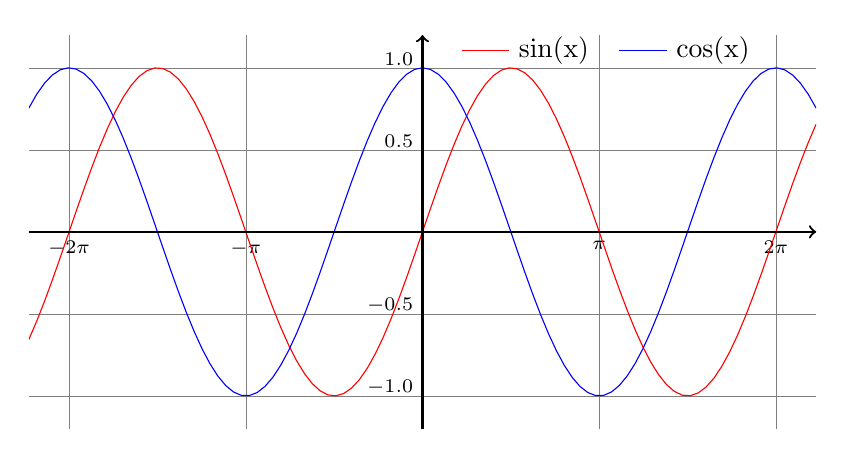
\begin{tikzpicture}[]
\begin{scope}[]
\clip (0.0,0.0) rectangle (10.0,5.0);
\begin{scope}[shift={(0.0,0.0)}]
\pgfsetxvec{\pgfpoint{0.71428573cm}{0cm}}
\pgfsetyvec{\pgfpoint{0cm}{2.0833333cm}}
\begin{scope}[shift={(7.0,1.2)}]
\begin{scope}[yshift=2.5cm]
\draw[ultra thin,gray] [shift={(-6.283185307179586,-1.2)}] (0,2.5cm) -- (0,-2.5cm) node[black,midway,below]{ \scriptsize{$-2\pi$}};
\draw[ultra thin,gray] [shift={(-3.141592653589793,-1.2)}] (0,2.5cm) -- (0,-2.5cm) node[black,midway,below]{ \scriptsize{$-\pi$}};
\draw[ultra thin,gray] [shift={(3.141592653589793,-1.2)}] (0,2.5cm) -- (0,-2.5cm) node[black,midway,below]{ \scriptsize{$\pi$}};
\draw[ultra thin,gray] [shift={(6.283185307179586,-1.2)}] (0,2.5cm) -- (0,-2.5cm) node[black,midway,below]{ \scriptsize{$2\pi$}};
\end{scope}
\begin{scope}[xshift=5cm]
\draw[ultra thin,gray] [shift={(-7.0,-1.0)}] (5cm,0) -- (-5cm,0) node[above=3pt,black,midway,left]{ \scriptsize{\num[round-mode=places,round-precision=1]{-1.0}}};
\draw[ultra thin,gray] [shift={(-7.0,-0.5)}] (5cm,0) -- (-5cm,0) node[above=3pt,black,midway,left]{ \scriptsize{\num[round-mode=places,round-precision=1]{-0.5}}};
\draw[ultra thin,gray] [shift={(-7.0,0.5)}] (5cm,0) -- (-5cm,0) node[above=3pt,black,midway,left]{ \scriptsize{\num[round-mode=places,round-precision=1]{0.5}}};
\draw[ultra thin,gray] [shift={(-7.0,1.0)}] (5cm,0) -- (-5cm,0) node[above=3pt,black,midway,left]{ \scriptsize{\num[round-mode=places,round-precision=1]{1.0}}};
\end{scope}
\begin{scope}[red]
\pgfpathmoveto{ \pgfqpointxy {-7.0} {-0.6569866}}
\pgfpathlineto{ \pgfqpointxy {-6.86} {-0.54535675}}
\pgfpathlineto{ \pgfqpointxy {-6.72} {-0.4230554}}
\pgfpathlineto{ \pgfqpointxy {-6.58} {-0.29247567}}
\pgfpathlineto{ \pgfqpointxy {-6.44} {-0.15617278}}
\pgfpathlineto{ \pgfqpointxy {-6.3} {-0.0168139}}
\pgfpathlineto{ \pgfqpointxy {-6.16} {0.12287399}}
\pgfpathlineto{ \pgfqpointxy {-6.02} {0.2601575}}
\pgfpathlineto{ \pgfqpointxy {-5.88} {0.39235023}}
\pgfpathlineto{ \pgfqpointxy {-5.74} {0.51686543}}
\pgfpathlineto{ \pgfqpointxy {-5.6} {0.63126665}}
\pgfpathlineto{ \pgfqpointxy {-5.46} {0.7333152}}
\pgfpathlineto{ \pgfqpointxy {-5.32} {0.8210142}}
\pgfpathlineto{ \pgfqpointxy {-5.18} {0.8926477}}
\pgfpathlineto{ \pgfqpointxy {-5.04} {0.94681376}}
\pgfpathlineto{ \pgfqpointxy {-4.9} {0.98245263}}
\pgfpathlineto{ \pgfqpointxy {-4.76} {0.9988668}}
\pgfpathlineto{ \pgfqpointxy {-4.62} {0.99573517}}
\pgfpathlineto{ \pgfqpointxy {-4.48} {0.97311896}}
\pgfpathlineto{ \pgfqpointxy {-4.34} {0.9314608}}
\pgfpathlineto{ \pgfqpointxy {-4.2} {0.8715758}}
\pgfpathlineto{ \pgfqpointxy {-4.06} {0.7946358}}
\pgfpathlineto{ \pgfqpointxy {-3.92} {0.7021463}}
\pgfpathlineto{ \pgfqpointxy {-3.78} {0.5959172}}
\pgfpathlineto{ \pgfqpointxy {-3.64} {0.47802725}}
\pgfpathlineto{ \pgfqpointxy {-3.5} {0.35078323}}
\pgfpathlineto{ \pgfqpointxy {-3.36} {0.21667509}}
\pgfpathlineto{ \pgfqpointxy {-3.22} {0.07832703}}
\pgfpathlineto{ \pgfqpointxy {-3.08} {-0.061553717}}
\pgfpathlineto{ \pgfqpointxy {-2.94} {-0.20022999}}
\pgfpathlineto{ \pgfqpointxy {-2.8} {-0.33498815}}
\pgfpathlineto{ \pgfqpointxy {-2.66} {-0.46319127}}
\pgfpathlineto{ \pgfqpointxy {-2.52} {-0.58233064}}
\pgfpathlineto{ \pgfqpointxy {-2.38} {-0.690075}}
\pgfpathlineto{ \pgfqpointxy {-2.24} {-0.78431594}}
\pgfpathlineto{ \pgfqpointxy {-2.1} {-0.86320937}}
\pgfpathlineto{ \pgfqpointxy {-1.96} {-0.92521155}}
\pgfpathlineto{ \pgfqpointxy {-1.82} {-0.9691091}}
\pgfpathlineto{ \pgfqpointxy {-1.68} {-0.99404323}}
\pgfpathlineto{ \pgfqpointxy {-1.54} {-0.99952585}}
\pgfpathlineto{ \pgfqpointxy {-1.4} {-0.98544973}}
\pgfpathlineto{ \pgfqpointxy {-1.26} {-0.9520903}}
\pgfpathlineto{ \pgfqpointxy {-1.12} {-0.90010047}}
\pgfpathlineto{ \pgfqpointxy {-0.98} {-0.8304974}}
\pgfpathlineto{ \pgfqpointxy {-0.84} {-0.7446431}}
\pgfpathlineto{ \pgfqpointxy {-0.7} {-0.64421767}}
\pgfpathlineto{ \pgfqpointxy {-0.56} {-0.5311862}}
\pgfpathlineto{ \pgfqpointxy {-0.42} {-0.40776044}}
\pgfpathlineto{ \pgfqpointxy {-0.28} {-0.27635565}}
\pgfpathlineto{ \pgfqpointxy {-0.14} {-0.13954312}}
\pgfpathlineto{ \pgfqpointxy {0.0} {0.0}}
\pgfpathlineto{ \pgfqpointxy {0.14} {0.13954312}}
\pgfpathlineto{ \pgfqpointxy {0.28} {0.27635565}}
\pgfpathlineto{ \pgfqpointxy {0.42} {0.40776044}}
\pgfpathlineto{ \pgfqpointxy {0.56} {0.5311862}}
\pgfpathlineto{ \pgfqpointxy {0.7} {0.64421767}}
\pgfpathlineto{ \pgfqpointxy {0.84} {0.7446431}}
\pgfpathlineto{ \pgfqpointxy {0.98} {0.8304974}}
\pgfpathlineto{ \pgfqpointxy {1.12} {0.90010047}}
\pgfpathlineto{ \pgfqpointxy {1.26} {0.9520903}}
\pgfpathlineto{ \pgfqpointxy {1.4} {0.98544973}}
\pgfpathlineto{ \pgfqpointxy {1.54} {0.99952585}}
\pgfpathlineto{ \pgfqpointxy {1.68} {0.99404323}}
\pgfpathlineto{ \pgfqpointxy {1.82} {0.9691091}}
\pgfpathlineto{ \pgfqpointxy {1.96} {0.92521155}}
\pgfpathlineto{ \pgfqpointxy {2.1} {0.86320937}}
\pgfpathlineto{ \pgfqpointxy {2.24} {0.78431594}}
\pgfpathlineto{ \pgfqpointxy {2.38} {0.690075}}
\pgfpathlineto{ \pgfqpointxy {2.52} {0.58233064}}
\pgfpathlineto{ \pgfqpointxy {2.66} {0.46319127}}
\pgfpathlineto{ \pgfqpointxy {2.8} {0.33498815}}
\pgfpathlineto{ \pgfqpointxy {2.94} {0.20022999}}
\pgfpathlineto{ \pgfqpointxy {3.08} {0.061553717}}
\pgfpathlineto{ \pgfqpointxy {3.22} {-0.07832703}}
\pgfpathlineto{ \pgfqpointxy {3.36} {-0.21667509}}
\pgfpathlineto{ \pgfqpointxy {3.5} {-0.35078323}}
\pgfpathlineto{ \pgfqpointxy {3.64} {-0.47802725}}
\pgfpathlineto{ \pgfqpointxy {3.78} {-0.5959172}}
\pgfpathlineto{ \pgfqpointxy {3.92} {-0.7021463}}
\pgfpathlineto{ \pgfqpointxy {4.06} {-0.7946358}}
\pgfpathlineto{ \pgfqpointxy {4.2} {-0.8715758}}
\pgfpathlineto{ \pgfqpointxy {4.34} {-0.9314608}}
\pgfpathlineto{ \pgfqpointxy {4.48} {-0.97311896}}
\pgfpathlineto{ \pgfqpointxy {4.62} {-0.99573517}}
\pgfpathlineto{ \pgfqpointxy {4.76} {-0.9988668}}
\pgfpathlineto{ \pgfqpointxy {4.9} {-0.98245263}}
\pgfpathlineto{ \pgfqpointxy {5.04} {-0.94681376}}
\pgfpathlineto{ \pgfqpointxy {5.18} {-0.8926477}}
\pgfpathlineto{ \pgfqpointxy {5.32} {-0.8210142}}
\pgfpathlineto{ \pgfqpointxy {5.46} {-0.7333152}}
\pgfpathlineto{ \pgfqpointxy {5.6} {-0.63126665}}
\pgfpathlineto{ \pgfqpointxy {5.74} {-0.51686543}}
\pgfpathlineto{ \pgfqpointxy {5.88} {-0.39235023}}
\pgfpathlineto{ \pgfqpointxy {6.02} {-0.2601575}}
\pgfpathlineto{ \pgfqpointxy {6.16} {-0.12287399}}
\pgfpathlineto{ \pgfqpointxy {6.3} {0.0168139}}
\pgfpathlineto{ \pgfqpointxy {6.44} {0.15617278}}
\pgfpathlineto{ \pgfqpointxy {6.58} {0.29247567}}
\pgfpathlineto{ \pgfqpointxy {6.72} {0.4230554}}
\pgfpathlineto{ \pgfqpointxy {6.86} {0.54535675}}
\pgfpathlineto{ \pgfqpointxy {7.0} {0.6569866}}
\pgfusepath{ stroke }
\end{scope}
\begin{scope}[blue]
\pgfpathmoveto{ \pgfqpointxy {-7.0} {0.75390226}}
\pgfpathlineto{ \pgfqpointxy {-6.86} {0.838204}}
\pgfpathlineto{ \pgfqpointxy {-6.72} {0.9061038}}
\pgfpathlineto{ \pgfqpointxy {-6.58} {0.95627296}}
\pgfpathlineto{ \pgfqpointxy {-6.44} {0.9877297}}
\pgfpathlineto{ \pgfqpointxy {-6.3} {0.9998586}}
\pgfpathlineto{ \pgfqpointxy {-6.16} {0.9924223}}
\pgfpathlineto{ \pgfqpointxy {-6.02} {0.9655662}}
\pgfpathlineto{ \pgfqpointxy {-5.88} {0.9198159}}
\pgfpathlineto{ \pgfqpointxy {-5.74} {0.85606664}}
\pgfpathlineto{ \pgfqpointxy {-5.6} {0.77556586}}
\pgfpathlineto{ \pgfqpointxy {-5.46} {0.67988884}}
\pgfpathlineto{ \pgfqpointxy {-5.32} {0.5709077}}
\pgfpathlineto{ \pgfqpointxy {-5.18} {0.45075506}}
\pgfpathlineto{ \pgfqpointxy {-5.04} {0.32178202}}
\pgfpathlineto{ \pgfqpointxy {-4.9} {0.18651237}}
\pgfpathlineto{ \pgfqpointxy {-4.76} {0.047593035}}
\pgfpathlineto{ \pgfqpointxy {-4.62} {-0.092257604}}
\pgfpathlineto{ \pgfqpointxy {-4.48} {-0.23030294}}
\pgfpathlineto{ \pgfqpointxy {-4.34} {-0.3638417}}
\pgfpathlineto{ \pgfqpointxy {-4.2} {-0.4902608}}
\pgfpathlineto{ \pgfqpointxy {-4.06} {-0.6070865}}
\pgfpathlineto{ \pgfqpointxy {-3.92} {-0.71203274}}
\pgfpathlineto{ \pgfqpointxy {-3.78} {-0.80304587}}
\pgfpathlineto{ \pgfqpointxy {-3.64} {-0.878345}}
\pgfpathlineto{ \pgfqpointxy {-3.5} {-0.9364567}}
\pgfpathlineto{ \pgfqpointxy {-3.36} {-0.9762438}}
\pgfpathlineto{ \pgfqpointxy {-3.22} {-0.99692774}}
\pgfpathlineto{ \pgfqpointxy {-3.08} {-0.9981038}}
\pgfpathlineto{ \pgfqpointxy {-2.94} {-0.9797489}}
\pgfpathlineto{ \pgfqpointxy {-2.8} {-0.94222236}}
\pgfpathlineto{ \pgfqpointxy {-2.66} {-0.88625836}}
\pgfpathlineto{ \pgfqpointxy {-2.52} {-0.81295204}}
\pgfpathlineto{ \pgfqpointxy {-2.38} {-0.7237379}}
\pgfpathlineto{ \pgfqpointxy {-2.24} {-0.6203616}}
\pgfpathlineto{ \pgfqpointxy {-2.1} {-0.5048461}}
\pgfpathlineto{ \pgfqpointxy {-1.96} {-0.37945175}}
\pgfpathlineto{ \pgfqpointxy {-1.82} {-0.24663231}}
\pgfpathlineto{ \pgfqpointxy {-1.68} {-0.10898675}}
\pgfpathlineto{ \pgfqpointxy {-1.54} {0.03079146}}
\pgfpathlineto{ \pgfqpointxy {-1.4} {0.16996714}}
\pgfpathlineto{ \pgfqpointxy {-1.26} {0.30581692}}
\pgfpathlineto{ \pgfqpointxy {-1.12} {0.43568245}}
\pgfpathlineto{ \pgfqpointxy {-0.98} {0.5570226}}
\pgfpathlineto{ \pgfqpointxy {-0.84} {0.6674628}}
\pgfpathlineto{ \pgfqpointxy {-0.7} {0.7648422}}
\pgfpathlineto{ \pgfqpointxy {-0.56} {0.8472551}}
\pgfpathlineto{ \pgfqpointxy {-0.42} {0.9130889}}
\pgfpathlineto{ \pgfqpointxy {-0.28} {0.96105546}}
\pgfpathlineto{ \pgfqpointxy {-0.14} {0.990216}}
\pgfpathlineto{ \pgfqpointxy {0.0} {1.0}}
\pgfpathlineto{ \pgfqpointxy {0.14} {0.990216}}
\pgfpathlineto{ \pgfqpointxy {0.28} {0.96105546}}
\pgfpathlineto{ \pgfqpointxy {0.42} {0.9130889}}
\pgfpathlineto{ \pgfqpointxy {0.56} {0.8472551}}
\pgfpathlineto{ \pgfqpointxy {0.7} {0.7648422}}
\pgfpathlineto{ \pgfqpointxy {0.84} {0.6674628}}
\pgfpathlineto{ \pgfqpointxy {0.98} {0.5570226}}
\pgfpathlineto{ \pgfqpointxy {1.12} {0.43568245}}
\pgfpathlineto{ \pgfqpointxy {1.26} {0.30581692}}
\pgfpathlineto{ \pgfqpointxy {1.4} {0.16996714}}
\pgfpathlineto{ \pgfqpointxy {1.54} {0.03079146}}
\pgfpathlineto{ \pgfqpointxy {1.68} {-0.10898675}}
\pgfpathlineto{ \pgfqpointxy {1.82} {-0.24663231}}
\pgfpathlineto{ \pgfqpointxy {1.96} {-0.37945175}}
\pgfpathlineto{ \pgfqpointxy {2.1} {-0.5048461}}
\pgfpathlineto{ \pgfqpointxy {2.24} {-0.6203616}}
\pgfpathlineto{ \pgfqpointxy {2.38} {-0.7237379}}
\pgfpathlineto{ \pgfqpointxy {2.52} {-0.81295204}}
\pgfpathlineto{ \pgfqpointxy {2.66} {-0.88625836}}
\pgfpathlineto{ \pgfqpointxy {2.8} {-0.94222236}}
\pgfpathlineto{ \pgfqpointxy {2.94} {-0.9797489}}
\pgfpathlineto{ \pgfqpointxy {3.08} {-0.9981038}}
\pgfpathlineto{ \pgfqpointxy {3.22} {-0.99692774}}
\pgfpathlineto{ \pgfqpointxy {3.36} {-0.9762438}}
\pgfpathlineto{ \pgfqpointxy {3.5} {-0.9364567}}
\pgfpathlineto{ \pgfqpointxy {3.64} {-0.878345}}
\pgfpathlineto{ \pgfqpointxy {3.78} {-0.80304587}}
\pgfpathlineto{ \pgfqpointxy {3.92} {-0.71203274}}
\pgfpathlineto{ \pgfqpointxy {4.06} {-0.6070865}}
\pgfpathlineto{ \pgfqpointxy {4.2} {-0.4902608}}
\pgfpathlineto{ \pgfqpointxy {4.34} {-0.3638417}}
\pgfpathlineto{ \pgfqpointxy {4.48} {-0.23030294}}
\pgfpathlineto{ \pgfqpointxy {4.62} {-0.092257604}}
\pgfpathlineto{ \pgfqpointxy {4.76} {0.047593035}}
\pgfpathlineto{ \pgfqpointxy {4.9} {0.18651237}}
\pgfpathlineto{ \pgfqpointxy {5.04} {0.32178202}}
\pgfpathlineto{ \pgfqpointxy {5.18} {0.45075506}}
\pgfpathlineto{ \pgfqpointxy {5.32} {0.5709077}}
\pgfpathlineto{ \pgfqpointxy {5.46} {0.67988884}}
\pgfpathlineto{ \pgfqpointxy {5.6} {0.77556586}}
\pgfpathlineto{ \pgfqpointxy {5.74} {0.85606664}}
\pgfpathlineto{ \pgfqpointxy {5.88} {0.9198159}}
\pgfpathlineto{ \pgfqpointxy {6.02} {0.9655662}}
\pgfpathlineto{ \pgfqpointxy {6.16} {0.9924223}}
\pgfpathlineto{ \pgfqpointxy {6.3} {0.9998586}}
\pgfpathlineto{ \pgfqpointxy {6.44} {0.9877297}}
\pgfpathlineto{ \pgfqpointxy {6.58} {0.95627296}}
\pgfpathlineto{ \pgfqpointxy {6.72} {0.9061038}}
\pgfpathlineto{ \pgfqpointxy {6.86} {0.838204}}
\pgfpathlineto{ \pgfqpointxy {7.0} {0.75390226}}
\pgfusepath{ stroke }
\end{scope}
\end{scope}
\pgfsetxvec{\pgfpoint{1cm}{0cm}}
\pgfsetyvec{\pgfpoint{0cm}{1cm}}
\end{scope}
\end{scope}
\draw[thick,->] (5.0,0.0) -- (5.0,5.0);
\draw[thick,->] (0.0,2.5) -- (10.0,2.5);
\draw[red] (5.5,4.8) -- (6.1,4.8);
\node[right,] at (6.1,4.8) {sin(x)};
\draw[blue] (7.5,4.8) -- (8.1,4.8);
\node[right,] at (8.1,4.8) {cos(x)};
\end{tikzpicture}
%%% Local Variables: 
%%% mode: latex 
%%% TeX-master: "master" 
%%% End:


  \caption{Plotting functions}
\end{figure}

\begin{figure}[H]
  \centering
  \documentclass{standalone}
\ifx\HCode\UnDef\else\def\pgfsysdriver{pgfsys-tex4ht.def}\fi
\usepackage{tikz}
\usepackage{color}
\usepackage{siunitx}
\usetikzlibrary{arrows,shapes}
\begin{document}
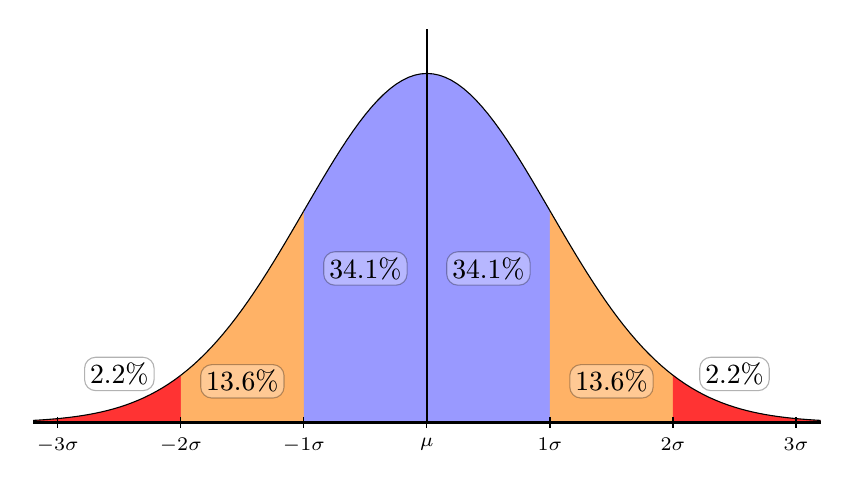
\begin{tikzpicture}
\begin{scope}[]
\pgfpathmoveto{ \pgfpointxy {0.0} {0.0}}
\pgfpathlineto{ \pgfpointxy {10.0} {0.0}}
\pgfpathlineto{ \pgfpointxy {10.0} {5.0}}
\pgfpathlineto{ \pgfpointxy {0.0} {5.0}}
\pgfpathclose
\pgfusepath{  clip, }
\begin{scope}[shift={(0.0,0.0)}]
\pgfsetxvec{\pgfpoint{1.5625cm}{0cm}}
\pgfsetyvec{\pgfpoint{0cm}{11.111112cm}}
\begin{scope}[shift={(3.2,0.0)}]
\begin{scope}[]
\pgfpathmoveto{ \pgfpointxy {-3.5} {0.0}}
\pgfpathlineto{ \pgfpointxy {-2.0} {0.0}}
\pgfpathlineto{ \pgfpointxy {-2.0} {5.0}}
\pgfpathlineto{ \pgfpointxy {-3.5} {5.0}}
\pgfpathclose
\pgfusepath{  clip, }
\begin{scope}[fill=red!80]
\pgfpathmoveto{ \pgfpointxy {-3.2} {0.0}}
\pgfpathlineto{ \pgfpointxy {-3.2} {0.0023840873753184963}}
\pgfpathlineto{ \pgfpointxy {-3.15} {0.002794257593560257}}
\pgfpathlineto{ \pgfpointxy {-3.1000001} {0.0032668180294884892}}
\pgfpathlineto{ \pgfpointxy {-3.05} {0.0038097626369961333}}
\pgfpathlineto{ \pgfpointxy {-3.0} {0.004431848335480958}}
\pgfpathlineto{ \pgfpointxy {-2.95} {0.005142640152435692}}
\pgfpathlineto{ \pgfpointxy {-2.9} {0.0059525301721895674}}
\pgfpathlineto{ \pgfpointxy {-2.8500001} {0.006872765030160735}}
\pgfpathlineto{ \pgfpointxy {-2.8} {0.007915452600647405}}
\pgfpathlineto{ \pgfpointxy {-2.75} {0.009093562739915748}}
\pgfpathlineto{ \pgfpointxy {-2.7} {0.010420932487815211}}
\pgfpathlineto{ \pgfpointxy {-2.65} {0.011912240802789813}}
\pgfpathlineto{ \pgfpointxy {-2.6} {0.013582973636746678}}
\pgfpathlineto{ \pgfpointxy {-2.55} {0.0154493503693536}}
\pgfpathlineto{ \pgfpointxy {-2.5} {0.017528300772314036}}
\pgfpathlineto{ \pgfpointxy {-2.45} {0.01983735428926949}}
\pgfpathlineto{ \pgfpointxy {-2.4} {0.022394527829526112}}
\pgfpathlineto{ \pgfpointxy {-2.35} {0.02521822470809983}}
\pgfpathlineto{ \pgfpointxy {-2.3} {0.028327036984334027}}
\pgfpathlineto{ \pgfpointxy {-2.25} {0.03173965331899954}}
\pgfpathlineto{ \pgfpointxy {-2.2} {0.03547459146264942}}
\pgfpathlineto{ \pgfpointxy {-2.15} {0.03955003329010437}}
\pgfpathlineto{ \pgfpointxy {-2.1} {0.043983610791136565}}
\pgfpathlineto{ \pgfpointxy {-2.0500002} {0.0487919988582986}}
\pgfpathlineto{ \pgfpointxy {-2.0} {0.05399096581690089}}
\pgfpathlineto{ \pgfpointxy {-1.95} {0.059594698701195395}}
\pgfpathlineto{ \pgfpointxy {-1.9} {0.0656158210884853}}
\pgfpathlineto{ \pgfpointxy {-1.85} {0.07206486699288937}}
\pgfpathlineto{ \pgfpointxy {-1.8000001} {0.07895014710951938}}
\pgfpathlineto{ \pgfpointxy {-1.75} {0.08627732079584774}}
\pgfpathlineto{ \pgfpointxy {-1.7} {0.09404907505773316}}
\pgfpathlineto{ \pgfpointxy {-1.65} {0.10226493431891748}}
\pgfpathlineto{ \pgfpointxy {-1.6} {0.11092082645768998}}
\pgfpathlineto{ \pgfpointxy {-1.5500001} {0.12000899363633905}}
\pgfpathlineto{ \pgfpointxy {-1.5} {0.12951759400603588}}
\pgfpathlineto{ \pgfpointxy {-1.45} {0.13943055308925387}}
\pgfpathlineto{ \pgfpointxy {-1.4} {0.1497274686645169}}
\pgfpathlineto{ \pgfpointxy {-1.35} {0.16038331353123803}}
\pgfpathlineto{ \pgfpointxy {-1.3000001} {0.1713685781825969}}
\pgfpathlineto{ \pgfpointxy {-1.25} {0.18264908057503657}}
\pgfpathlineto{ \pgfpointxy {-1.2} {0.19418604935410852}}
\pgfpathlineto{ \pgfpointxy {-1.1500001} {0.20593624274853736}}
\pgfpathlineto{ \pgfpointxy {-1.0999999} {0.2178522101371628}}
\pgfpathlineto{ \pgfpointxy {-1.05} {0.22988214937606208}}
\pgfpathlineto{ \pgfpointxy {-1.0} {0.24197072716759546}}
\pgfpathlineto{ \pgfpointxy {-0.95000005} {0.2540590433921869}}
\pgfpathlineto{ \pgfpointxy {-0.9000001} {0.2660852255786465}}
\pgfpathlineto{ \pgfpointxy {-0.8499999} {0.2779849044804291}}
\pgfpathlineto{ \pgfpointxy {-0.79999995} {0.28969157075782764}}
\pgfpathlineto{ \pgfpointxy {-0.75} {0.301137431015238}}
\pgfpathlineto{ \pgfpointxy {-0.70000005} {0.3122539309350428}}
\pgfpathlineto{ \pgfpointxy {-0.6500001} {0.3229723497479345}}
\pgfpathlineto{ \pgfpointxy {-0.5999999} {0.33322460871255405}}
\pgfpathlineto{ \pgfpointxy {-0.54999995} {0.3429438655858136}}
\pgfpathlineto{ \pgfpointxy {-0.5} {0.3520653231025355}}
\pgfpathlineto{ \pgfpointxy {-0.45000005} {0.3605269661186527}}
\pgfpathlineto{ \pgfpointxy {-0.4000001} {0.368270132302718}}
\pgfpathlineto{ \pgfpointxy {-0.3499999} {0.3752403681731694}}
\pgfpathlineto{ \pgfpointxy {-0.29999995} {0.38138780955933627}}
\pgfpathlineto{ \pgfpointxy {-0.25} {0.3866681089751429}}
\pgfpathlineto{ \pgfpointxy {-0.20000005} {0.39104269718605056}}
\pgfpathlineto{ \pgfpointxy {-0.1500001} {0.3944793301217544}}
\pgfpathlineto{ \pgfpointxy {-0.099999905} {0.3969525406736286}}
\pgfpathlineto{ \pgfpointxy {-0.049999952} {0.39844392404048146}}
\pgfpathlineto{ \pgfpointxy {0.0} {0.3989422804014327}}
\pgfpathlineto{ \pgfpointxy {0.049999952} {0.39844392404048146}}
\pgfpathlineto{ \pgfpointxy {0.099999905} {0.3969525406736286}}
\pgfpathlineto{ \pgfpointxy {0.1500001} {0.3944793301217544}}
\pgfpathlineto{ \pgfpointxy {0.20000005} {0.39104269718605056}}
\pgfpathlineto{ \pgfpointxy {0.25} {0.3866681089751429}}
\pgfpathlineto{ \pgfpointxy {0.29999995} {0.38138780955933627}}
\pgfpathlineto{ \pgfpointxy {0.3499999} {0.3752403681731694}}
\pgfpathlineto{ \pgfpointxy {0.4000001} {0.368270132302718}}
\pgfpathlineto{ \pgfpointxy {0.45000005} {0.3605269661186527}}
\pgfpathlineto{ \pgfpointxy {0.5} {0.3520653231025355}}
\pgfpathlineto{ \pgfpointxy {0.54999995} {0.3429438655858136}}
\pgfpathlineto{ \pgfpointxy {0.5999999} {0.33322460871255405}}
\pgfpathlineto{ \pgfpointxy {0.6500001} {0.3229723497479345}}
\pgfpathlineto{ \pgfpointxy {0.70000005} {0.3122539309350428}}
\pgfpathlineto{ \pgfpointxy {0.75} {0.301137431015238}}
\pgfpathlineto{ \pgfpointxy {0.79999995} {0.28969157075782764}}
\pgfpathlineto{ \pgfpointxy {0.85000014} {0.2779848569228033}}
\pgfpathlineto{ \pgfpointxy {0.89999986} {0.2660852731362723}}
\pgfpathlineto{ \pgfpointxy {0.95000005} {0.2540590433921869}}
\pgfpathlineto{ \pgfpointxy {1.0000002} {0.24197065583115673}}
\pgfpathlineto{ \pgfpointxy {1.05} {0.22988214937606208}}
\pgfpathlineto{ \pgfpointxy {1.1000001} {0.21785213880072407}}
\pgfpathlineto{ \pgfpointxy {1.1499999} {0.2059363140849761}}
\pgfpathlineto{ \pgfpointxy {1.2} {0.19418604935410852}}
\pgfpathlineto{ \pgfpointxy {1.2500002} {0.18264903301741073}}
\pgfpathlineto{ \pgfpointxy {1.3} {0.1713686019614098}}
\pgfpathlineto{ \pgfpointxy {1.3500001} {0.16038330164183157}}
\pgfpathlineto{ \pgfpointxy {1.3999999} {0.14972750433273627}}
\pgfpathlineto{ \pgfpointxy {1.45} {0.13943055308925387}}
\pgfpathlineto{ \pgfpointxy {1.5000002} {0.12951754644841007}}
\pgfpathlineto{ \pgfpointxy {1.55} {0.1200090055257455}}
\pgfpathlineto{ \pgfpointxy {1.6000001} {0.11092081456828352}}
\pgfpathlineto{ \pgfpointxy {1.6499999} {0.10226494620832394}}
\pgfpathlineto{ \pgfpointxy {1.7} {0.09404907505773316}}
\pgfpathlineto{ \pgfpointxy {1.7500002} {0.08627727918292515}}
\pgfpathlineto{ \pgfpointxy {1.8} {0.07895016494362907}}
\pgfpathlineto{ \pgfpointxy {1.8500001} {0.07206485510348291}}
\pgfpathlineto{ \pgfpointxy {1.8999999} {0.06561583297789175}}
\pgfpathlineto{ \pgfpointxy {1.95} {0.059594698701195395}}
\pgfpathlineto{ \pgfpointxy {2.0000002} {0.053990942038087984}}
\pgfpathlineto{ \pgfpointxy {2.05} {0.048792022637111514}}
\pgfpathlineto{ \pgfpointxy {2.1000001} {0.043983578095268816}}
\pgfpathlineto{ \pgfpointxy {2.1499999} {0.03955005112421405}}
\pgfpathlineto{ \pgfpointxy {2.2} {0.03547459146264942}}
\pgfpathlineto{ \pgfpointxy {2.2500002} {0.03173963548488986}}
\pgfpathlineto{ \pgfpointxy {2.3} {0.028327036984334027}}
\pgfpathlineto{ \pgfpointxy {2.3500001} {0.025218212818693374}}
\pgfpathlineto{ \pgfpointxy {2.3999999} {0.02239453823275676}}
\pgfpathlineto{ \pgfpointxy {2.45} {0.01983735428926949}}
\pgfpathlineto{ \pgfpointxy {2.5000002} {0.017528287396731772}}
\pgfpathlineto{ \pgfpointxy {2.55} {0.0154493503693536}}
\pgfpathlineto{ \pgfpointxy {2.6000001} {0.013582964719691839}}
\pgfpathlineto{ \pgfpointxy {2.6499999} {0.01191224897675675}}
\pgfpathlineto{ \pgfpointxy {2.7} {0.010420932487815211}}
\pgfpathlineto{ \pgfpointxy {2.7500002} {0.009093556052124616}}
\pgfpathlineto{ \pgfpointxy {2.8} {0.007915452600647405}}
\pgfpathlineto{ \pgfpointxy {2.8500001} {0.006872765030160735}}
\pgfpathlineto{ \pgfpointxy {2.8999999} {0.005952535745348843}}
\pgfpathlineto{ \pgfpointxy {2.95} {0.005142640152435692}}
\pgfpathlineto{ \pgfpointxy {3.0000002} {0.004431844248497489}}
\pgfpathlineto{ \pgfpointxy {3.05} {0.0038097626369961333}}
\pgfpathlineto{ \pgfpointxy {3.1000001} {0.0032668180294884892}}
\pgfpathlineto{ \pgfpointxy {3.1499999} {0.0027942601943679187}}
\pgfpathlineto{ \pgfpointxy {3.2} {0.0023840873753184963}}
\pgfpathlineto{ \pgfpointxy {3.2} {0.0}}
\pgfusepath{ stroke, fill, }
\end{scope}
\end{scope}
\node at (-2.5,0.05546041322884499) [rectangle,inner sep=2.0pt,minimum width =2.0pt,minimum height=2.0pt,fill=white,opacity=0.3,draw=black, rounded corners] {2.2\%}; 
\node at (-2.5,0.05546041322884499) [rectangle,inner sep=0.0pt,minimum width =2.0pt,minimum height=2.0pt,text=black] {2.2\%}; 
\end{scope}
\pgfsetxvec{\pgfpoint{1cm}{0cm}}
\pgfsetyvec{\pgfpoint{0cm}{1cm}}
\end{scope}
\end{scope}
\begin{scope}[]
\pgfpathmoveto{ \pgfpointxy {0.0} {0.0}}
\pgfpathlineto{ \pgfpointxy {10.0} {0.0}}
\pgfpathlineto{ \pgfpointxy {10.0} {5.0}}
\pgfpathlineto{ \pgfpointxy {0.0} {5.0}}
\pgfpathclose
\pgfusepath{  clip, }
\begin{scope}[shift={(0.0,0.0)}]
\pgfsetxvec{\pgfpoint{1.5625cm}{0cm}}
\pgfsetyvec{\pgfpoint{0cm}{11.111112cm}}
\begin{scope}[shift={(3.2,0.0)}]
\begin{scope}[]
\pgfpathmoveto{ \pgfpointxy {-2.0} {0.0}}
\pgfpathlineto{ \pgfpointxy {-1.0} {0.0}}
\pgfpathlineto{ \pgfpointxy {-1.0} {5.0}}
\pgfpathlineto{ \pgfpointxy {-2.0} {5.0}}
\pgfpathclose
\pgfusepath{  clip, }
\begin{scope}[fill=orange!60]
\pgfpathmoveto{ \pgfpointxy {-3.2} {0.0}}
\pgfpathlineto{ \pgfpointxy {-3.2} {0.0023840873753184963}}
\pgfpathlineto{ \pgfpointxy {-3.15} {0.002794257593560257}}
\pgfpathlineto{ \pgfpointxy {-3.1000001} {0.0032668180294884892}}
\pgfpathlineto{ \pgfpointxy {-3.05} {0.0038097626369961333}}
\pgfpathlineto{ \pgfpointxy {-3.0} {0.004431848335480958}}
\pgfpathlineto{ \pgfpointxy {-2.95} {0.005142640152435692}}
\pgfpathlineto{ \pgfpointxy {-2.9} {0.0059525301721895674}}
\pgfpathlineto{ \pgfpointxy {-2.8500001} {0.006872765030160735}}
\pgfpathlineto{ \pgfpointxy {-2.8} {0.007915452600647405}}
\pgfpathlineto{ \pgfpointxy {-2.75} {0.009093562739915748}}
\pgfpathlineto{ \pgfpointxy {-2.7} {0.010420932487815211}}
\pgfpathlineto{ \pgfpointxy {-2.65} {0.011912240802789813}}
\pgfpathlineto{ \pgfpointxy {-2.6} {0.013582973636746678}}
\pgfpathlineto{ \pgfpointxy {-2.55} {0.0154493503693536}}
\pgfpathlineto{ \pgfpointxy {-2.5} {0.017528300772314036}}
\pgfpathlineto{ \pgfpointxy {-2.45} {0.01983735428926949}}
\pgfpathlineto{ \pgfpointxy {-2.4} {0.022394527829526112}}
\pgfpathlineto{ \pgfpointxy {-2.35} {0.02521822470809983}}
\pgfpathlineto{ \pgfpointxy {-2.3} {0.028327036984334027}}
\pgfpathlineto{ \pgfpointxy {-2.25} {0.03173965331899954}}
\pgfpathlineto{ \pgfpointxy {-2.2} {0.03547459146264942}}
\pgfpathlineto{ \pgfpointxy {-2.15} {0.03955003329010437}}
\pgfpathlineto{ \pgfpointxy {-2.1} {0.043983610791136565}}
\pgfpathlineto{ \pgfpointxy {-2.0500002} {0.0487919988582986}}
\pgfpathlineto{ \pgfpointxy {-2.0} {0.05399096581690089}}
\pgfpathlineto{ \pgfpointxy {-1.95} {0.059594698701195395}}
\pgfpathlineto{ \pgfpointxy {-1.9} {0.0656158210884853}}
\pgfpathlineto{ \pgfpointxy {-1.85} {0.07206486699288937}}
\pgfpathlineto{ \pgfpointxy {-1.8000001} {0.07895014710951938}}
\pgfpathlineto{ \pgfpointxy {-1.75} {0.08627732079584774}}
\pgfpathlineto{ \pgfpointxy {-1.7} {0.09404907505773316}}
\pgfpathlineto{ \pgfpointxy {-1.65} {0.10226493431891748}}
\pgfpathlineto{ \pgfpointxy {-1.6} {0.11092082645768998}}
\pgfpathlineto{ \pgfpointxy {-1.5500001} {0.12000899363633905}}
\pgfpathlineto{ \pgfpointxy {-1.5} {0.12951759400603588}}
\pgfpathlineto{ \pgfpointxy {-1.45} {0.13943055308925387}}
\pgfpathlineto{ \pgfpointxy {-1.4} {0.1497274686645169}}
\pgfpathlineto{ \pgfpointxy {-1.35} {0.16038331353123803}}
\pgfpathlineto{ \pgfpointxy {-1.3000001} {0.1713685781825969}}
\pgfpathlineto{ \pgfpointxy {-1.25} {0.18264908057503657}}
\pgfpathlineto{ \pgfpointxy {-1.2} {0.19418604935410852}}
\pgfpathlineto{ \pgfpointxy {-1.1500001} {0.20593624274853736}}
\pgfpathlineto{ \pgfpointxy {-1.0999999} {0.2178522101371628}}
\pgfpathlineto{ \pgfpointxy {-1.05} {0.22988214937606208}}
\pgfpathlineto{ \pgfpointxy {-1.0} {0.24197072716759546}}
\pgfpathlineto{ \pgfpointxy {-0.95000005} {0.2540590433921869}}
\pgfpathlineto{ \pgfpointxy {-0.9000001} {0.2660852255786465}}
\pgfpathlineto{ \pgfpointxy {-0.8499999} {0.2779849044804291}}
\pgfpathlineto{ \pgfpointxy {-0.79999995} {0.28969157075782764}}
\pgfpathlineto{ \pgfpointxy {-0.75} {0.301137431015238}}
\pgfpathlineto{ \pgfpointxy {-0.70000005} {0.3122539309350428}}
\pgfpathlineto{ \pgfpointxy {-0.6500001} {0.3229723497479345}}
\pgfpathlineto{ \pgfpointxy {-0.5999999} {0.33322460871255405}}
\pgfpathlineto{ \pgfpointxy {-0.54999995} {0.3429438655858136}}
\pgfpathlineto{ \pgfpointxy {-0.5} {0.3520653231025355}}
\pgfpathlineto{ \pgfpointxy {-0.45000005} {0.3605269661186527}}
\pgfpathlineto{ \pgfpointxy {-0.4000001} {0.368270132302718}}
\pgfpathlineto{ \pgfpointxy {-0.3499999} {0.3752403681731694}}
\pgfpathlineto{ \pgfpointxy {-0.29999995} {0.38138780955933627}}
\pgfpathlineto{ \pgfpointxy {-0.25} {0.3866681089751429}}
\pgfpathlineto{ \pgfpointxy {-0.20000005} {0.39104269718605056}}
\pgfpathlineto{ \pgfpointxy {-0.1500001} {0.3944793301217544}}
\pgfpathlineto{ \pgfpointxy {-0.099999905} {0.3969525406736286}}
\pgfpathlineto{ \pgfpointxy {-0.049999952} {0.39844392404048146}}
\pgfpathlineto{ \pgfpointxy {0.0} {0.3989422804014327}}
\pgfpathlineto{ \pgfpointxy {0.049999952} {0.39844392404048146}}
\pgfpathlineto{ \pgfpointxy {0.099999905} {0.3969525406736286}}
\pgfpathlineto{ \pgfpointxy {0.1500001} {0.3944793301217544}}
\pgfpathlineto{ \pgfpointxy {0.20000005} {0.39104269718605056}}
\pgfpathlineto{ \pgfpointxy {0.25} {0.3866681089751429}}
\pgfpathlineto{ \pgfpointxy {0.29999995} {0.38138780955933627}}
\pgfpathlineto{ \pgfpointxy {0.3499999} {0.3752403681731694}}
\pgfpathlineto{ \pgfpointxy {0.4000001} {0.368270132302718}}
\pgfpathlineto{ \pgfpointxy {0.45000005} {0.3605269661186527}}
\pgfpathlineto{ \pgfpointxy {0.5} {0.3520653231025355}}
\pgfpathlineto{ \pgfpointxy {0.54999995} {0.3429438655858136}}
\pgfpathlineto{ \pgfpointxy {0.5999999} {0.33322460871255405}}
\pgfpathlineto{ \pgfpointxy {0.6500001} {0.3229723497479345}}
\pgfpathlineto{ \pgfpointxy {0.70000005} {0.3122539309350428}}
\pgfpathlineto{ \pgfpointxy {0.75} {0.301137431015238}}
\pgfpathlineto{ \pgfpointxy {0.79999995} {0.28969157075782764}}
\pgfpathlineto{ \pgfpointxy {0.85000014} {0.2779848569228033}}
\pgfpathlineto{ \pgfpointxy {0.89999986} {0.2660852731362723}}
\pgfpathlineto{ \pgfpointxy {0.95000005} {0.2540590433921869}}
\pgfpathlineto{ \pgfpointxy {1.0000002} {0.24197065583115673}}
\pgfpathlineto{ \pgfpointxy {1.05} {0.22988214937606208}}
\pgfpathlineto{ \pgfpointxy {1.1000001} {0.21785213880072407}}
\pgfpathlineto{ \pgfpointxy {1.1499999} {0.2059363140849761}}
\pgfpathlineto{ \pgfpointxy {1.2} {0.19418604935410852}}
\pgfpathlineto{ \pgfpointxy {1.2500002} {0.18264903301741073}}
\pgfpathlineto{ \pgfpointxy {1.3} {0.1713686019614098}}
\pgfpathlineto{ \pgfpointxy {1.3500001} {0.16038330164183157}}
\pgfpathlineto{ \pgfpointxy {1.3999999} {0.14972750433273627}}
\pgfpathlineto{ \pgfpointxy {1.45} {0.13943055308925387}}
\pgfpathlineto{ \pgfpointxy {1.5000002} {0.12951754644841007}}
\pgfpathlineto{ \pgfpointxy {1.55} {0.1200090055257455}}
\pgfpathlineto{ \pgfpointxy {1.6000001} {0.11092081456828352}}
\pgfpathlineto{ \pgfpointxy {1.6499999} {0.10226494620832394}}
\pgfpathlineto{ \pgfpointxy {1.7} {0.09404907505773316}}
\pgfpathlineto{ \pgfpointxy {1.7500002} {0.08627727918292515}}
\pgfpathlineto{ \pgfpointxy {1.8} {0.07895016494362907}}
\pgfpathlineto{ \pgfpointxy {1.8500001} {0.07206485510348291}}
\pgfpathlineto{ \pgfpointxy {1.8999999} {0.06561583297789175}}
\pgfpathlineto{ \pgfpointxy {1.95} {0.059594698701195395}}
\pgfpathlineto{ \pgfpointxy {2.0000002} {0.053990942038087984}}
\pgfpathlineto{ \pgfpointxy {2.05} {0.048792022637111514}}
\pgfpathlineto{ \pgfpointxy {2.1000001} {0.043983578095268816}}
\pgfpathlineto{ \pgfpointxy {2.1499999} {0.03955005112421405}}
\pgfpathlineto{ \pgfpointxy {2.2} {0.03547459146264942}}
\pgfpathlineto{ \pgfpointxy {2.2500002} {0.03173963548488986}}
\pgfpathlineto{ \pgfpointxy {2.3} {0.028327036984334027}}
\pgfpathlineto{ \pgfpointxy {2.3500001} {0.025218212818693374}}
\pgfpathlineto{ \pgfpointxy {2.3999999} {0.02239453823275676}}
\pgfpathlineto{ \pgfpointxy {2.45} {0.01983735428926949}}
\pgfpathlineto{ \pgfpointxy {2.5000002} {0.017528287396731772}}
\pgfpathlineto{ \pgfpointxy {2.55} {0.0154493503693536}}
\pgfpathlineto{ \pgfpointxy {2.6000001} {0.013582964719691839}}
\pgfpathlineto{ \pgfpointxy {2.6499999} {0.01191224897675675}}
\pgfpathlineto{ \pgfpointxy {2.7} {0.010420932487815211}}
\pgfpathlineto{ \pgfpointxy {2.7500002} {0.009093556052124616}}
\pgfpathlineto{ \pgfpointxy {2.8} {0.007915452600647405}}
\pgfpathlineto{ \pgfpointxy {2.8500001} {0.006872765030160735}}
\pgfpathlineto{ \pgfpointxy {2.8999999} {0.005952535745348843}}
\pgfpathlineto{ \pgfpointxy {2.95} {0.005142640152435692}}
\pgfpathlineto{ \pgfpointxy {3.0000002} {0.004431844248497489}}
\pgfpathlineto{ \pgfpointxy {3.05} {0.0038097626369961333}}
\pgfpathlineto{ \pgfpointxy {3.1000001} {0.0032668180294884892}}
\pgfpathlineto{ \pgfpointxy {3.1499999} {0.0027942601943679187}}
\pgfpathlineto{ \pgfpointxy {3.2} {0.0023840873753184963}}
\pgfpathlineto{ \pgfpointxy {3.2} {0.0}}
\pgfusepath{ stroke, fill, }
\end{scope}
\end{scope}
\node at (-1.5,0.04702453752886658) [rectangle,inner sep=2.0pt,minimum width =2.0pt,minimum height=2.0pt,fill=white,opacity=0.3,draw=black, rounded corners] {13.6\%}; 
\node at (-1.5,0.04702453752886658) [rectangle,inner sep=0.0pt,minimum width =2.0pt,minimum height=2.0pt,text=black] {13.6\%}; 
\end{scope}
\pgfsetxvec{\pgfpoint{1cm}{0cm}}
\pgfsetyvec{\pgfpoint{0cm}{1cm}}
\end{scope}
\end{scope}
\begin{scope}[]
\pgfpathmoveto{ \pgfpointxy {0.0} {0.0}}
\pgfpathlineto{ \pgfpointxy {10.0} {0.0}}
\pgfpathlineto{ \pgfpointxy {10.0} {5.0}}
\pgfpathlineto{ \pgfpointxy {0.0} {5.0}}
\pgfpathclose
\pgfusepath{  clip, }
\begin{scope}[shift={(0.0,0.0)}]
\pgfsetxvec{\pgfpoint{1.5625cm}{0cm}}
\pgfsetyvec{\pgfpoint{0cm}{11.111112cm}}
\begin{scope}[shift={(3.2,0.0)}]
\begin{scope}[]
\pgfpathmoveto{ \pgfpointxy {-1.0} {0.0}}
\pgfpathlineto{ \pgfpointxy {0.0} {0.0}}
\pgfpathlineto{ \pgfpointxy {0.0} {5.0}}
\pgfpathlineto{ \pgfpointxy {-1.0} {5.0}}
\pgfpathclose
\pgfusepath{  clip, }
\begin{scope}[fill=blue!40]
\pgfpathmoveto{ \pgfpointxy {-3.2} {0.0}}
\pgfpathlineto{ \pgfpointxy {-3.2} {0.0023840873753184963}}
\pgfpathlineto{ \pgfpointxy {-3.15} {0.002794257593560257}}
\pgfpathlineto{ \pgfpointxy {-3.1000001} {0.0032668180294884892}}
\pgfpathlineto{ \pgfpointxy {-3.05} {0.0038097626369961333}}
\pgfpathlineto{ \pgfpointxy {-3.0} {0.004431848335480958}}
\pgfpathlineto{ \pgfpointxy {-2.95} {0.005142640152435692}}
\pgfpathlineto{ \pgfpointxy {-2.9} {0.0059525301721895674}}
\pgfpathlineto{ \pgfpointxy {-2.8500001} {0.006872765030160735}}
\pgfpathlineto{ \pgfpointxy {-2.8} {0.007915452600647405}}
\pgfpathlineto{ \pgfpointxy {-2.75} {0.009093562739915748}}
\pgfpathlineto{ \pgfpointxy {-2.7} {0.010420932487815211}}
\pgfpathlineto{ \pgfpointxy {-2.65} {0.011912240802789813}}
\pgfpathlineto{ \pgfpointxy {-2.6} {0.013582973636746678}}
\pgfpathlineto{ \pgfpointxy {-2.55} {0.0154493503693536}}
\pgfpathlineto{ \pgfpointxy {-2.5} {0.017528300772314036}}
\pgfpathlineto{ \pgfpointxy {-2.45} {0.01983735428926949}}
\pgfpathlineto{ \pgfpointxy {-2.4} {0.022394527829526112}}
\pgfpathlineto{ \pgfpointxy {-2.35} {0.02521822470809983}}
\pgfpathlineto{ \pgfpointxy {-2.3} {0.028327036984334027}}
\pgfpathlineto{ \pgfpointxy {-2.25} {0.03173965331899954}}
\pgfpathlineto{ \pgfpointxy {-2.2} {0.03547459146264942}}
\pgfpathlineto{ \pgfpointxy {-2.15} {0.03955003329010437}}
\pgfpathlineto{ \pgfpointxy {-2.1} {0.043983610791136565}}
\pgfpathlineto{ \pgfpointxy {-2.0500002} {0.0487919988582986}}
\pgfpathlineto{ \pgfpointxy {-2.0} {0.05399096581690089}}
\pgfpathlineto{ \pgfpointxy {-1.95} {0.059594698701195395}}
\pgfpathlineto{ \pgfpointxy {-1.9} {0.0656158210884853}}
\pgfpathlineto{ \pgfpointxy {-1.85} {0.07206486699288937}}
\pgfpathlineto{ \pgfpointxy {-1.8000001} {0.07895014710951938}}
\pgfpathlineto{ \pgfpointxy {-1.75} {0.08627732079584774}}
\pgfpathlineto{ \pgfpointxy {-1.7} {0.09404907505773316}}
\pgfpathlineto{ \pgfpointxy {-1.65} {0.10226493431891748}}
\pgfpathlineto{ \pgfpointxy {-1.6} {0.11092082645768998}}
\pgfpathlineto{ \pgfpointxy {-1.5500001} {0.12000899363633905}}
\pgfpathlineto{ \pgfpointxy {-1.5} {0.12951759400603588}}
\pgfpathlineto{ \pgfpointxy {-1.45} {0.13943055308925387}}
\pgfpathlineto{ \pgfpointxy {-1.4} {0.1497274686645169}}
\pgfpathlineto{ \pgfpointxy {-1.35} {0.16038331353123803}}
\pgfpathlineto{ \pgfpointxy {-1.3000001} {0.1713685781825969}}
\pgfpathlineto{ \pgfpointxy {-1.25} {0.18264908057503657}}
\pgfpathlineto{ \pgfpointxy {-1.2} {0.19418604935410852}}
\pgfpathlineto{ \pgfpointxy {-1.1500001} {0.20593624274853736}}
\pgfpathlineto{ \pgfpointxy {-1.0999999} {0.2178522101371628}}
\pgfpathlineto{ \pgfpointxy {-1.05} {0.22988214937606208}}
\pgfpathlineto{ \pgfpointxy {-1.0} {0.24197072716759546}}
\pgfpathlineto{ \pgfpointxy {-0.95000005} {0.2540590433921869}}
\pgfpathlineto{ \pgfpointxy {-0.9000001} {0.2660852255786465}}
\pgfpathlineto{ \pgfpointxy {-0.8499999} {0.2779849044804291}}
\pgfpathlineto{ \pgfpointxy {-0.79999995} {0.28969157075782764}}
\pgfpathlineto{ \pgfpointxy {-0.75} {0.301137431015238}}
\pgfpathlineto{ \pgfpointxy {-0.70000005} {0.3122539309350428}}
\pgfpathlineto{ \pgfpointxy {-0.6500001} {0.3229723497479345}}
\pgfpathlineto{ \pgfpointxy {-0.5999999} {0.33322460871255405}}
\pgfpathlineto{ \pgfpointxy {-0.54999995} {0.3429438655858136}}
\pgfpathlineto{ \pgfpointxy {-0.5} {0.3520653231025355}}
\pgfpathlineto{ \pgfpointxy {-0.45000005} {0.3605269661186527}}
\pgfpathlineto{ \pgfpointxy {-0.4000001} {0.368270132302718}}
\pgfpathlineto{ \pgfpointxy {-0.3499999} {0.3752403681731694}}
\pgfpathlineto{ \pgfpointxy {-0.29999995} {0.38138780955933627}}
\pgfpathlineto{ \pgfpointxy {-0.25} {0.3866681089751429}}
\pgfpathlineto{ \pgfpointxy {-0.20000005} {0.39104269718605056}}
\pgfpathlineto{ \pgfpointxy {-0.1500001} {0.3944793301217544}}
\pgfpathlineto{ \pgfpointxy {-0.099999905} {0.3969525406736286}}
\pgfpathlineto{ \pgfpointxy {-0.049999952} {0.39844392404048146}}
\pgfpathlineto{ \pgfpointxy {0.0} {0.3989422804014327}}
\pgfpathlineto{ \pgfpointxy {0.049999952} {0.39844392404048146}}
\pgfpathlineto{ \pgfpointxy {0.099999905} {0.3969525406736286}}
\pgfpathlineto{ \pgfpointxy {0.1500001} {0.3944793301217544}}
\pgfpathlineto{ \pgfpointxy {0.20000005} {0.39104269718605056}}
\pgfpathlineto{ \pgfpointxy {0.25} {0.3866681089751429}}
\pgfpathlineto{ \pgfpointxy {0.29999995} {0.38138780955933627}}
\pgfpathlineto{ \pgfpointxy {0.3499999} {0.3752403681731694}}
\pgfpathlineto{ \pgfpointxy {0.4000001} {0.368270132302718}}
\pgfpathlineto{ \pgfpointxy {0.45000005} {0.3605269661186527}}
\pgfpathlineto{ \pgfpointxy {0.5} {0.3520653231025355}}
\pgfpathlineto{ \pgfpointxy {0.54999995} {0.3429438655858136}}
\pgfpathlineto{ \pgfpointxy {0.5999999} {0.33322460871255405}}
\pgfpathlineto{ \pgfpointxy {0.6500001} {0.3229723497479345}}
\pgfpathlineto{ \pgfpointxy {0.70000005} {0.3122539309350428}}
\pgfpathlineto{ \pgfpointxy {0.75} {0.301137431015238}}
\pgfpathlineto{ \pgfpointxy {0.79999995} {0.28969157075782764}}
\pgfpathlineto{ \pgfpointxy {0.85000014} {0.2779848569228033}}
\pgfpathlineto{ \pgfpointxy {0.89999986} {0.2660852731362723}}
\pgfpathlineto{ \pgfpointxy {0.95000005} {0.2540590433921869}}
\pgfpathlineto{ \pgfpointxy {1.0000002} {0.24197065583115673}}
\pgfpathlineto{ \pgfpointxy {1.05} {0.22988214937606208}}
\pgfpathlineto{ \pgfpointxy {1.1000001} {0.21785213880072407}}
\pgfpathlineto{ \pgfpointxy {1.1499999} {0.2059363140849761}}
\pgfpathlineto{ \pgfpointxy {1.2} {0.19418604935410852}}
\pgfpathlineto{ \pgfpointxy {1.2500002} {0.18264903301741073}}
\pgfpathlineto{ \pgfpointxy {1.3} {0.1713686019614098}}
\pgfpathlineto{ \pgfpointxy {1.3500001} {0.16038330164183157}}
\pgfpathlineto{ \pgfpointxy {1.3999999} {0.14972750433273627}}
\pgfpathlineto{ \pgfpointxy {1.45} {0.13943055308925387}}
\pgfpathlineto{ \pgfpointxy {1.5000002} {0.12951754644841007}}
\pgfpathlineto{ \pgfpointxy {1.55} {0.1200090055257455}}
\pgfpathlineto{ \pgfpointxy {1.6000001} {0.11092081456828352}}
\pgfpathlineto{ \pgfpointxy {1.6499999} {0.10226494620832394}}
\pgfpathlineto{ \pgfpointxy {1.7} {0.09404907505773316}}
\pgfpathlineto{ \pgfpointxy {1.7500002} {0.08627727918292515}}
\pgfpathlineto{ \pgfpointxy {1.8} {0.07895016494362907}}
\pgfpathlineto{ \pgfpointxy {1.8500001} {0.07206485510348291}}
\pgfpathlineto{ \pgfpointxy {1.8999999} {0.06561583297789175}}
\pgfpathlineto{ \pgfpointxy {1.95} {0.059594698701195395}}
\pgfpathlineto{ \pgfpointxy {2.0000002} {0.053990942038087984}}
\pgfpathlineto{ \pgfpointxy {2.05} {0.048792022637111514}}
\pgfpathlineto{ \pgfpointxy {2.1000001} {0.043983578095268816}}
\pgfpathlineto{ \pgfpointxy {2.1499999} {0.03955005112421405}}
\pgfpathlineto{ \pgfpointxy {2.2} {0.03547459146264942}}
\pgfpathlineto{ \pgfpointxy {2.2500002} {0.03173963548488986}}
\pgfpathlineto{ \pgfpointxy {2.3} {0.028327036984334027}}
\pgfpathlineto{ \pgfpointxy {2.3500001} {0.025218212818693374}}
\pgfpathlineto{ \pgfpointxy {2.3999999} {0.02239453823275676}}
\pgfpathlineto{ \pgfpointxy {2.45} {0.01983735428926949}}
\pgfpathlineto{ \pgfpointxy {2.5000002} {0.017528287396731772}}
\pgfpathlineto{ \pgfpointxy {2.55} {0.0154493503693536}}
\pgfpathlineto{ \pgfpointxy {2.6000001} {0.013582964719691839}}
\pgfpathlineto{ \pgfpointxy {2.6499999} {0.01191224897675675}}
\pgfpathlineto{ \pgfpointxy {2.7} {0.010420932487815211}}
\pgfpathlineto{ \pgfpointxy {2.7500002} {0.009093556052124616}}
\pgfpathlineto{ \pgfpointxy {2.8} {0.007915452600647405}}
\pgfpathlineto{ \pgfpointxy {2.8500001} {0.006872765030160735}}
\pgfpathlineto{ \pgfpointxy {2.8999999} {0.005952535745348843}}
\pgfpathlineto{ \pgfpointxy {2.95} {0.005142640152435692}}
\pgfpathlineto{ \pgfpointxy {3.0000002} {0.004431844248497489}}
\pgfpathlineto{ \pgfpointxy {3.05} {0.0038097626369961333}}
\pgfpathlineto{ \pgfpointxy {3.1000001} {0.0032668180294884892}}
\pgfpathlineto{ \pgfpointxy {3.1499999} {0.0027942601943679187}}
\pgfpathlineto{ \pgfpointxy {3.2} {0.0023840873753184963}}
\pgfpathlineto{ \pgfpointxy {3.2} {0.0}}
\pgfusepath{ stroke, fill, }
\end{scope}
\end{scope}
\node at (-0.5,0.17603266155126776) [rectangle,inner sep=2.0pt,minimum width =2.0pt,minimum height=2.0pt,fill=white,opacity=0.3,draw=black, rounded corners] {34.1\%}; 
\node at (-0.5,0.17603266155126776) [rectangle,inner sep=0.0pt,minimum width =2.0pt,minimum height=2.0pt,text=black] {34.1\%}; 
\end{scope}
\pgfsetxvec{\pgfpoint{1cm}{0cm}}
\pgfsetyvec{\pgfpoint{0cm}{1cm}}
\end{scope}
\end{scope}
\begin{scope}[]
\pgfpathmoveto{ \pgfpointxy {0.0} {0.0}}
\pgfpathlineto{ \pgfpointxy {10.0} {0.0}}
\pgfpathlineto{ \pgfpointxy {10.0} {5.0}}
\pgfpathlineto{ \pgfpointxy {0.0} {5.0}}
\pgfpathclose
\pgfusepath{  clip, }
\begin{scope}[shift={(0.0,0.0)}]
\pgfsetxvec{\pgfpoint{1.5625cm}{0cm}}
\pgfsetyvec{\pgfpoint{0cm}{11.111112cm}}
\begin{scope}[shift={(3.2,0.0)}]
\begin{scope}[]
\pgfpathmoveto{ \pgfpointxy {0.0} {0.0}}
\pgfpathlineto{ \pgfpointxy {1.0} {0.0}}
\pgfpathlineto{ \pgfpointxy {1.0} {5.0}}
\pgfpathlineto{ \pgfpointxy {0.0} {5.0}}
\pgfpathclose
\pgfusepath{  clip, }
\begin{scope}[fill=blue!40]
\pgfpathmoveto{ \pgfpointxy {-3.2} {0.0}}
\pgfpathlineto{ \pgfpointxy {-3.2} {0.0023840873753184963}}
\pgfpathlineto{ \pgfpointxy {-3.15} {0.002794257593560257}}
\pgfpathlineto{ \pgfpointxy {-3.1000001} {0.0032668180294884892}}
\pgfpathlineto{ \pgfpointxy {-3.05} {0.0038097626369961333}}
\pgfpathlineto{ \pgfpointxy {-3.0} {0.004431848335480958}}
\pgfpathlineto{ \pgfpointxy {-2.95} {0.005142640152435692}}
\pgfpathlineto{ \pgfpointxy {-2.9} {0.0059525301721895674}}
\pgfpathlineto{ \pgfpointxy {-2.8500001} {0.006872765030160735}}
\pgfpathlineto{ \pgfpointxy {-2.8} {0.007915452600647405}}
\pgfpathlineto{ \pgfpointxy {-2.75} {0.009093562739915748}}
\pgfpathlineto{ \pgfpointxy {-2.7} {0.010420932487815211}}
\pgfpathlineto{ \pgfpointxy {-2.65} {0.011912240802789813}}
\pgfpathlineto{ \pgfpointxy {-2.6} {0.013582973636746678}}
\pgfpathlineto{ \pgfpointxy {-2.55} {0.0154493503693536}}
\pgfpathlineto{ \pgfpointxy {-2.5} {0.017528300772314036}}
\pgfpathlineto{ \pgfpointxy {-2.45} {0.01983735428926949}}
\pgfpathlineto{ \pgfpointxy {-2.4} {0.022394527829526112}}
\pgfpathlineto{ \pgfpointxy {-2.35} {0.02521822470809983}}
\pgfpathlineto{ \pgfpointxy {-2.3} {0.028327036984334027}}
\pgfpathlineto{ \pgfpointxy {-2.25} {0.03173965331899954}}
\pgfpathlineto{ \pgfpointxy {-2.2} {0.03547459146264942}}
\pgfpathlineto{ \pgfpointxy {-2.15} {0.03955003329010437}}
\pgfpathlineto{ \pgfpointxy {-2.1} {0.043983610791136565}}
\pgfpathlineto{ \pgfpointxy {-2.0500002} {0.0487919988582986}}
\pgfpathlineto{ \pgfpointxy {-2.0} {0.05399096581690089}}
\pgfpathlineto{ \pgfpointxy {-1.95} {0.059594698701195395}}
\pgfpathlineto{ \pgfpointxy {-1.9} {0.0656158210884853}}
\pgfpathlineto{ \pgfpointxy {-1.85} {0.07206486699288937}}
\pgfpathlineto{ \pgfpointxy {-1.8000001} {0.07895014710951938}}
\pgfpathlineto{ \pgfpointxy {-1.75} {0.08627732079584774}}
\pgfpathlineto{ \pgfpointxy {-1.7} {0.09404907505773316}}
\pgfpathlineto{ \pgfpointxy {-1.65} {0.10226493431891748}}
\pgfpathlineto{ \pgfpointxy {-1.6} {0.11092082645768998}}
\pgfpathlineto{ \pgfpointxy {-1.5500001} {0.12000899363633905}}
\pgfpathlineto{ \pgfpointxy {-1.5} {0.12951759400603588}}
\pgfpathlineto{ \pgfpointxy {-1.45} {0.13943055308925387}}
\pgfpathlineto{ \pgfpointxy {-1.4} {0.1497274686645169}}
\pgfpathlineto{ \pgfpointxy {-1.35} {0.16038331353123803}}
\pgfpathlineto{ \pgfpointxy {-1.3000001} {0.1713685781825969}}
\pgfpathlineto{ \pgfpointxy {-1.25} {0.18264908057503657}}
\pgfpathlineto{ \pgfpointxy {-1.2} {0.19418604935410852}}
\pgfpathlineto{ \pgfpointxy {-1.1500001} {0.20593624274853736}}
\pgfpathlineto{ \pgfpointxy {-1.0999999} {0.2178522101371628}}
\pgfpathlineto{ \pgfpointxy {-1.05} {0.22988214937606208}}
\pgfpathlineto{ \pgfpointxy {-1.0} {0.24197072716759546}}
\pgfpathlineto{ \pgfpointxy {-0.95000005} {0.2540590433921869}}
\pgfpathlineto{ \pgfpointxy {-0.9000001} {0.2660852255786465}}
\pgfpathlineto{ \pgfpointxy {-0.8499999} {0.2779849044804291}}
\pgfpathlineto{ \pgfpointxy {-0.79999995} {0.28969157075782764}}
\pgfpathlineto{ \pgfpointxy {-0.75} {0.301137431015238}}
\pgfpathlineto{ \pgfpointxy {-0.70000005} {0.3122539309350428}}
\pgfpathlineto{ \pgfpointxy {-0.6500001} {0.3229723497479345}}
\pgfpathlineto{ \pgfpointxy {-0.5999999} {0.33322460871255405}}
\pgfpathlineto{ \pgfpointxy {-0.54999995} {0.3429438655858136}}
\pgfpathlineto{ \pgfpointxy {-0.5} {0.3520653231025355}}
\pgfpathlineto{ \pgfpointxy {-0.45000005} {0.3605269661186527}}
\pgfpathlineto{ \pgfpointxy {-0.4000001} {0.368270132302718}}
\pgfpathlineto{ \pgfpointxy {-0.3499999} {0.3752403681731694}}
\pgfpathlineto{ \pgfpointxy {-0.29999995} {0.38138780955933627}}
\pgfpathlineto{ \pgfpointxy {-0.25} {0.3866681089751429}}
\pgfpathlineto{ \pgfpointxy {-0.20000005} {0.39104269718605056}}
\pgfpathlineto{ \pgfpointxy {-0.1500001} {0.3944793301217544}}
\pgfpathlineto{ \pgfpointxy {-0.099999905} {0.3969525406736286}}
\pgfpathlineto{ \pgfpointxy {-0.049999952} {0.39844392404048146}}
\pgfpathlineto{ \pgfpointxy {0.0} {0.3989422804014327}}
\pgfpathlineto{ \pgfpointxy {0.049999952} {0.39844392404048146}}
\pgfpathlineto{ \pgfpointxy {0.099999905} {0.3969525406736286}}
\pgfpathlineto{ \pgfpointxy {0.1500001} {0.3944793301217544}}
\pgfpathlineto{ \pgfpointxy {0.20000005} {0.39104269718605056}}
\pgfpathlineto{ \pgfpointxy {0.25} {0.3866681089751429}}
\pgfpathlineto{ \pgfpointxy {0.29999995} {0.38138780955933627}}
\pgfpathlineto{ \pgfpointxy {0.3499999} {0.3752403681731694}}
\pgfpathlineto{ \pgfpointxy {0.4000001} {0.368270132302718}}
\pgfpathlineto{ \pgfpointxy {0.45000005} {0.3605269661186527}}
\pgfpathlineto{ \pgfpointxy {0.5} {0.3520653231025355}}
\pgfpathlineto{ \pgfpointxy {0.54999995} {0.3429438655858136}}
\pgfpathlineto{ \pgfpointxy {0.5999999} {0.33322460871255405}}
\pgfpathlineto{ \pgfpointxy {0.6500001} {0.3229723497479345}}
\pgfpathlineto{ \pgfpointxy {0.70000005} {0.3122539309350428}}
\pgfpathlineto{ \pgfpointxy {0.75} {0.301137431015238}}
\pgfpathlineto{ \pgfpointxy {0.79999995} {0.28969157075782764}}
\pgfpathlineto{ \pgfpointxy {0.85000014} {0.2779848569228033}}
\pgfpathlineto{ \pgfpointxy {0.89999986} {0.2660852731362723}}
\pgfpathlineto{ \pgfpointxy {0.95000005} {0.2540590433921869}}
\pgfpathlineto{ \pgfpointxy {1.0000002} {0.24197065583115673}}
\pgfpathlineto{ \pgfpointxy {1.05} {0.22988214937606208}}
\pgfpathlineto{ \pgfpointxy {1.1000001} {0.21785213880072407}}
\pgfpathlineto{ \pgfpointxy {1.1499999} {0.2059363140849761}}
\pgfpathlineto{ \pgfpointxy {1.2} {0.19418604935410852}}
\pgfpathlineto{ \pgfpointxy {1.2500002} {0.18264903301741073}}
\pgfpathlineto{ \pgfpointxy {1.3} {0.1713686019614098}}
\pgfpathlineto{ \pgfpointxy {1.3500001} {0.16038330164183157}}
\pgfpathlineto{ \pgfpointxy {1.3999999} {0.14972750433273627}}
\pgfpathlineto{ \pgfpointxy {1.45} {0.13943055308925387}}
\pgfpathlineto{ \pgfpointxy {1.5000002} {0.12951754644841007}}
\pgfpathlineto{ \pgfpointxy {1.55} {0.1200090055257455}}
\pgfpathlineto{ \pgfpointxy {1.6000001} {0.11092081456828352}}
\pgfpathlineto{ \pgfpointxy {1.6499999} {0.10226494620832394}}
\pgfpathlineto{ \pgfpointxy {1.7} {0.09404907505773316}}
\pgfpathlineto{ \pgfpointxy {1.7500002} {0.08627727918292515}}
\pgfpathlineto{ \pgfpointxy {1.8} {0.07895016494362907}}
\pgfpathlineto{ \pgfpointxy {1.8500001} {0.07206485510348291}}
\pgfpathlineto{ \pgfpointxy {1.8999999} {0.06561583297789175}}
\pgfpathlineto{ \pgfpointxy {1.95} {0.059594698701195395}}
\pgfpathlineto{ \pgfpointxy {2.0000002} {0.053990942038087984}}
\pgfpathlineto{ \pgfpointxy {2.05} {0.048792022637111514}}
\pgfpathlineto{ \pgfpointxy {2.1000001} {0.043983578095268816}}
\pgfpathlineto{ \pgfpointxy {2.1499999} {0.03955005112421405}}
\pgfpathlineto{ \pgfpointxy {2.2} {0.03547459146264942}}
\pgfpathlineto{ \pgfpointxy {2.2500002} {0.03173963548488986}}
\pgfpathlineto{ \pgfpointxy {2.3} {0.028327036984334027}}
\pgfpathlineto{ \pgfpointxy {2.3500001} {0.025218212818693374}}
\pgfpathlineto{ \pgfpointxy {2.3999999} {0.02239453823275676}}
\pgfpathlineto{ \pgfpointxy {2.45} {0.01983735428926949}}
\pgfpathlineto{ \pgfpointxy {2.5000002} {0.017528287396731772}}
\pgfpathlineto{ \pgfpointxy {2.55} {0.0154493503693536}}
\pgfpathlineto{ \pgfpointxy {2.6000001} {0.013582964719691839}}
\pgfpathlineto{ \pgfpointxy {2.6499999} {0.01191224897675675}}
\pgfpathlineto{ \pgfpointxy {2.7} {0.010420932487815211}}
\pgfpathlineto{ \pgfpointxy {2.7500002} {0.009093556052124616}}
\pgfpathlineto{ \pgfpointxy {2.8} {0.007915452600647405}}
\pgfpathlineto{ \pgfpointxy {2.8500001} {0.006872765030160735}}
\pgfpathlineto{ \pgfpointxy {2.8999999} {0.005952535745348843}}
\pgfpathlineto{ \pgfpointxy {2.95} {0.005142640152435692}}
\pgfpathlineto{ \pgfpointxy {3.0000002} {0.004431844248497489}}
\pgfpathlineto{ \pgfpointxy {3.05} {0.0038097626369961333}}
\pgfpathlineto{ \pgfpointxy {3.1000001} {0.0032668180294884892}}
\pgfpathlineto{ \pgfpointxy {3.1499999} {0.0027942601943679187}}
\pgfpathlineto{ \pgfpointxy {3.2} {0.0023840873753184963}}
\pgfpathlineto{ \pgfpointxy {3.2} {0.0}}
\pgfusepath{ stroke, fill, }
\end{scope}
\end{scope}
\node at (0.5,0.17603266155126776) [rectangle,inner sep=2.0pt,minimum width =2.0pt,minimum height=2.0pt,fill=white,opacity=0.3,draw=black, rounded corners] {34.1\%}; 
\node at (0.5,0.17603266155126776) [rectangle,inner sep=0.0pt,minimum width =2.0pt,minimum height=2.0pt,text=black] {34.1\%}; 
\end{scope}
\pgfsetxvec{\pgfpoint{1cm}{0cm}}
\pgfsetyvec{\pgfpoint{0cm}{1cm}}
\end{scope}
\end{scope}
\begin{scope}[]
\pgfpathmoveto{ \pgfpointxy {0.0} {0.0}}
\pgfpathlineto{ \pgfpointxy {10.0} {0.0}}
\pgfpathlineto{ \pgfpointxy {10.0} {5.0}}
\pgfpathlineto{ \pgfpointxy {0.0} {5.0}}
\pgfpathclose
\pgfusepath{  clip, }
\begin{scope}[shift={(0.0,0.0)}]
\pgfsetxvec{\pgfpoint{1.5625cm}{0cm}}
\pgfsetyvec{\pgfpoint{0cm}{11.111112cm}}
\begin{scope}[shift={(3.2,0.0)}]
\begin{scope}[]
\pgfpathmoveto{ \pgfpointxy {1.0} {0.0}}
\pgfpathlineto{ \pgfpointxy {2.0} {0.0}}
\pgfpathlineto{ \pgfpointxy {2.0} {5.0}}
\pgfpathlineto{ \pgfpointxy {1.0} {5.0}}
\pgfpathclose
\pgfusepath{  clip, }
\begin{scope}[fill=orange!60]
\pgfpathmoveto{ \pgfpointxy {-3.2} {0.0}}
\pgfpathlineto{ \pgfpointxy {-3.2} {0.0023840873753184963}}
\pgfpathlineto{ \pgfpointxy {-3.15} {0.002794257593560257}}
\pgfpathlineto{ \pgfpointxy {-3.1000001} {0.0032668180294884892}}
\pgfpathlineto{ \pgfpointxy {-3.05} {0.0038097626369961333}}
\pgfpathlineto{ \pgfpointxy {-3.0} {0.004431848335480958}}
\pgfpathlineto{ \pgfpointxy {-2.95} {0.005142640152435692}}
\pgfpathlineto{ \pgfpointxy {-2.9} {0.0059525301721895674}}
\pgfpathlineto{ \pgfpointxy {-2.8500001} {0.006872765030160735}}
\pgfpathlineto{ \pgfpointxy {-2.8} {0.007915452600647405}}
\pgfpathlineto{ \pgfpointxy {-2.75} {0.009093562739915748}}
\pgfpathlineto{ \pgfpointxy {-2.7} {0.010420932487815211}}
\pgfpathlineto{ \pgfpointxy {-2.65} {0.011912240802789813}}
\pgfpathlineto{ \pgfpointxy {-2.6} {0.013582973636746678}}
\pgfpathlineto{ \pgfpointxy {-2.55} {0.0154493503693536}}
\pgfpathlineto{ \pgfpointxy {-2.5} {0.017528300772314036}}
\pgfpathlineto{ \pgfpointxy {-2.45} {0.01983735428926949}}
\pgfpathlineto{ \pgfpointxy {-2.4} {0.022394527829526112}}
\pgfpathlineto{ \pgfpointxy {-2.35} {0.02521822470809983}}
\pgfpathlineto{ \pgfpointxy {-2.3} {0.028327036984334027}}
\pgfpathlineto{ \pgfpointxy {-2.25} {0.03173965331899954}}
\pgfpathlineto{ \pgfpointxy {-2.2} {0.03547459146264942}}
\pgfpathlineto{ \pgfpointxy {-2.15} {0.03955003329010437}}
\pgfpathlineto{ \pgfpointxy {-2.1} {0.043983610791136565}}
\pgfpathlineto{ \pgfpointxy {-2.0500002} {0.0487919988582986}}
\pgfpathlineto{ \pgfpointxy {-2.0} {0.05399096581690089}}
\pgfpathlineto{ \pgfpointxy {-1.95} {0.059594698701195395}}
\pgfpathlineto{ \pgfpointxy {-1.9} {0.0656158210884853}}
\pgfpathlineto{ \pgfpointxy {-1.85} {0.07206486699288937}}
\pgfpathlineto{ \pgfpointxy {-1.8000001} {0.07895014710951938}}
\pgfpathlineto{ \pgfpointxy {-1.75} {0.08627732079584774}}
\pgfpathlineto{ \pgfpointxy {-1.7} {0.09404907505773316}}
\pgfpathlineto{ \pgfpointxy {-1.65} {0.10226493431891748}}
\pgfpathlineto{ \pgfpointxy {-1.6} {0.11092082645768998}}
\pgfpathlineto{ \pgfpointxy {-1.5500001} {0.12000899363633905}}
\pgfpathlineto{ \pgfpointxy {-1.5} {0.12951759400603588}}
\pgfpathlineto{ \pgfpointxy {-1.45} {0.13943055308925387}}
\pgfpathlineto{ \pgfpointxy {-1.4} {0.1497274686645169}}
\pgfpathlineto{ \pgfpointxy {-1.35} {0.16038331353123803}}
\pgfpathlineto{ \pgfpointxy {-1.3000001} {0.1713685781825969}}
\pgfpathlineto{ \pgfpointxy {-1.25} {0.18264908057503657}}
\pgfpathlineto{ \pgfpointxy {-1.2} {0.19418604935410852}}
\pgfpathlineto{ \pgfpointxy {-1.1500001} {0.20593624274853736}}
\pgfpathlineto{ \pgfpointxy {-1.0999999} {0.2178522101371628}}
\pgfpathlineto{ \pgfpointxy {-1.05} {0.22988214937606208}}
\pgfpathlineto{ \pgfpointxy {-1.0} {0.24197072716759546}}
\pgfpathlineto{ \pgfpointxy {-0.95000005} {0.2540590433921869}}
\pgfpathlineto{ \pgfpointxy {-0.9000001} {0.2660852255786465}}
\pgfpathlineto{ \pgfpointxy {-0.8499999} {0.2779849044804291}}
\pgfpathlineto{ \pgfpointxy {-0.79999995} {0.28969157075782764}}
\pgfpathlineto{ \pgfpointxy {-0.75} {0.301137431015238}}
\pgfpathlineto{ \pgfpointxy {-0.70000005} {0.3122539309350428}}
\pgfpathlineto{ \pgfpointxy {-0.6500001} {0.3229723497479345}}
\pgfpathlineto{ \pgfpointxy {-0.5999999} {0.33322460871255405}}
\pgfpathlineto{ \pgfpointxy {-0.54999995} {0.3429438655858136}}
\pgfpathlineto{ \pgfpointxy {-0.5} {0.3520653231025355}}
\pgfpathlineto{ \pgfpointxy {-0.45000005} {0.3605269661186527}}
\pgfpathlineto{ \pgfpointxy {-0.4000001} {0.368270132302718}}
\pgfpathlineto{ \pgfpointxy {-0.3499999} {0.3752403681731694}}
\pgfpathlineto{ \pgfpointxy {-0.29999995} {0.38138780955933627}}
\pgfpathlineto{ \pgfpointxy {-0.25} {0.3866681089751429}}
\pgfpathlineto{ \pgfpointxy {-0.20000005} {0.39104269718605056}}
\pgfpathlineto{ \pgfpointxy {-0.1500001} {0.3944793301217544}}
\pgfpathlineto{ \pgfpointxy {-0.099999905} {0.3969525406736286}}
\pgfpathlineto{ \pgfpointxy {-0.049999952} {0.39844392404048146}}
\pgfpathlineto{ \pgfpointxy {0.0} {0.3989422804014327}}
\pgfpathlineto{ \pgfpointxy {0.049999952} {0.39844392404048146}}
\pgfpathlineto{ \pgfpointxy {0.099999905} {0.3969525406736286}}
\pgfpathlineto{ \pgfpointxy {0.1500001} {0.3944793301217544}}
\pgfpathlineto{ \pgfpointxy {0.20000005} {0.39104269718605056}}
\pgfpathlineto{ \pgfpointxy {0.25} {0.3866681089751429}}
\pgfpathlineto{ \pgfpointxy {0.29999995} {0.38138780955933627}}
\pgfpathlineto{ \pgfpointxy {0.3499999} {0.3752403681731694}}
\pgfpathlineto{ \pgfpointxy {0.4000001} {0.368270132302718}}
\pgfpathlineto{ \pgfpointxy {0.45000005} {0.3605269661186527}}
\pgfpathlineto{ \pgfpointxy {0.5} {0.3520653231025355}}
\pgfpathlineto{ \pgfpointxy {0.54999995} {0.3429438655858136}}
\pgfpathlineto{ \pgfpointxy {0.5999999} {0.33322460871255405}}
\pgfpathlineto{ \pgfpointxy {0.6500001} {0.3229723497479345}}
\pgfpathlineto{ \pgfpointxy {0.70000005} {0.3122539309350428}}
\pgfpathlineto{ \pgfpointxy {0.75} {0.301137431015238}}
\pgfpathlineto{ \pgfpointxy {0.79999995} {0.28969157075782764}}
\pgfpathlineto{ \pgfpointxy {0.85000014} {0.2779848569228033}}
\pgfpathlineto{ \pgfpointxy {0.89999986} {0.2660852731362723}}
\pgfpathlineto{ \pgfpointxy {0.95000005} {0.2540590433921869}}
\pgfpathlineto{ \pgfpointxy {1.0000002} {0.24197065583115673}}
\pgfpathlineto{ \pgfpointxy {1.05} {0.22988214937606208}}
\pgfpathlineto{ \pgfpointxy {1.1000001} {0.21785213880072407}}
\pgfpathlineto{ \pgfpointxy {1.1499999} {0.2059363140849761}}
\pgfpathlineto{ \pgfpointxy {1.2} {0.19418604935410852}}
\pgfpathlineto{ \pgfpointxy {1.2500002} {0.18264903301741073}}
\pgfpathlineto{ \pgfpointxy {1.3} {0.1713686019614098}}
\pgfpathlineto{ \pgfpointxy {1.3500001} {0.16038330164183157}}
\pgfpathlineto{ \pgfpointxy {1.3999999} {0.14972750433273627}}
\pgfpathlineto{ \pgfpointxy {1.45} {0.13943055308925387}}
\pgfpathlineto{ \pgfpointxy {1.5000002} {0.12951754644841007}}
\pgfpathlineto{ \pgfpointxy {1.55} {0.1200090055257455}}
\pgfpathlineto{ \pgfpointxy {1.6000001} {0.11092081456828352}}
\pgfpathlineto{ \pgfpointxy {1.6499999} {0.10226494620832394}}
\pgfpathlineto{ \pgfpointxy {1.7} {0.09404907505773316}}
\pgfpathlineto{ \pgfpointxy {1.7500002} {0.08627727918292515}}
\pgfpathlineto{ \pgfpointxy {1.8} {0.07895016494362907}}
\pgfpathlineto{ \pgfpointxy {1.8500001} {0.07206485510348291}}
\pgfpathlineto{ \pgfpointxy {1.8999999} {0.06561583297789175}}
\pgfpathlineto{ \pgfpointxy {1.95} {0.059594698701195395}}
\pgfpathlineto{ \pgfpointxy {2.0000002} {0.053990942038087984}}
\pgfpathlineto{ \pgfpointxy {2.05} {0.048792022637111514}}
\pgfpathlineto{ \pgfpointxy {2.1000001} {0.043983578095268816}}
\pgfpathlineto{ \pgfpointxy {2.1499999} {0.03955005112421405}}
\pgfpathlineto{ \pgfpointxy {2.2} {0.03547459146264942}}
\pgfpathlineto{ \pgfpointxy {2.2500002} {0.03173963548488986}}
\pgfpathlineto{ \pgfpointxy {2.3} {0.028327036984334027}}
\pgfpathlineto{ \pgfpointxy {2.3500001} {0.025218212818693374}}
\pgfpathlineto{ \pgfpointxy {2.3999999} {0.02239453823275676}}
\pgfpathlineto{ \pgfpointxy {2.45} {0.01983735428926949}}
\pgfpathlineto{ \pgfpointxy {2.5000002} {0.017528287396731772}}
\pgfpathlineto{ \pgfpointxy {2.55} {0.0154493503693536}}
\pgfpathlineto{ \pgfpointxy {2.6000001} {0.013582964719691839}}
\pgfpathlineto{ \pgfpointxy {2.6499999} {0.01191224897675675}}
\pgfpathlineto{ \pgfpointxy {2.7} {0.010420932487815211}}
\pgfpathlineto{ \pgfpointxy {2.7500002} {0.009093556052124616}}
\pgfpathlineto{ \pgfpointxy {2.8} {0.007915452600647405}}
\pgfpathlineto{ \pgfpointxy {2.8500001} {0.006872765030160735}}
\pgfpathlineto{ \pgfpointxy {2.8999999} {0.005952535745348843}}
\pgfpathlineto{ \pgfpointxy {2.95} {0.005142640152435692}}
\pgfpathlineto{ \pgfpointxy {3.0000002} {0.004431844248497489}}
\pgfpathlineto{ \pgfpointxy {3.05} {0.0038097626369961333}}
\pgfpathlineto{ \pgfpointxy {3.1000001} {0.0032668180294884892}}
\pgfpathlineto{ \pgfpointxy {3.1499999} {0.0027942601943679187}}
\pgfpathlineto{ \pgfpointxy {3.2} {0.0023840873753184963}}
\pgfpathlineto{ \pgfpointxy {3.2} {0.0}}
\pgfusepath{ stroke, fill, }
\end{scope}
\end{scope}
\node at (1.5,0.04702453752886658) [rectangle,inner sep=2.0pt,minimum width =2.0pt,minimum height=2.0pt,fill=white,opacity=0.3,draw=black, rounded corners] {13.6\%}; 
\node at (1.5,0.04702453752886658) [rectangle,inner sep=0.0pt,minimum width =2.0pt,minimum height=2.0pt,text=black] {13.6\%}; 
\end{scope}
\pgfsetxvec{\pgfpoint{1cm}{0cm}}
\pgfsetyvec{\pgfpoint{0cm}{1cm}}
\end{scope}
\end{scope}
\begin{scope}[]
\pgfpathmoveto{ \pgfpointxy {0.0} {0.0}}
\pgfpathlineto{ \pgfpointxy {10.0} {0.0}}
\pgfpathlineto{ \pgfpointxy {10.0} {5.0}}
\pgfpathlineto{ \pgfpointxy {0.0} {5.0}}
\pgfpathclose
\pgfusepath{  clip, }
\begin{scope}[shift={(0.0,0.0)}]
\pgfsetxvec{\pgfpoint{1.5625cm}{0cm}}
\pgfsetyvec{\pgfpoint{0cm}{11.111112cm}}
\begin{scope}[shift={(3.2,0.0)}]
\begin{scope}[]
\pgfpathmoveto{ \pgfpointxy {2.0} {0.0}}
\pgfpathlineto{ \pgfpointxy {3.5} {0.0}}
\pgfpathlineto{ \pgfpointxy {3.5} {5.0}}
\pgfpathlineto{ \pgfpointxy {2.0} {5.0}}
\pgfpathclose
\pgfusepath{  clip, }
\begin{scope}[fill=red!80]
\pgfpathmoveto{ \pgfpointxy {-3.2} {0.0}}
\pgfpathlineto{ \pgfpointxy {-3.2} {0.0023840873753184963}}
\pgfpathlineto{ \pgfpointxy {-3.15} {0.002794257593560257}}
\pgfpathlineto{ \pgfpointxy {-3.1000001} {0.0032668180294884892}}
\pgfpathlineto{ \pgfpointxy {-3.05} {0.0038097626369961333}}
\pgfpathlineto{ \pgfpointxy {-3.0} {0.004431848335480958}}
\pgfpathlineto{ \pgfpointxy {-2.95} {0.005142640152435692}}
\pgfpathlineto{ \pgfpointxy {-2.9} {0.0059525301721895674}}
\pgfpathlineto{ \pgfpointxy {-2.8500001} {0.006872765030160735}}
\pgfpathlineto{ \pgfpointxy {-2.8} {0.007915452600647405}}
\pgfpathlineto{ \pgfpointxy {-2.75} {0.009093562739915748}}
\pgfpathlineto{ \pgfpointxy {-2.7} {0.010420932487815211}}
\pgfpathlineto{ \pgfpointxy {-2.65} {0.011912240802789813}}
\pgfpathlineto{ \pgfpointxy {-2.6} {0.013582973636746678}}
\pgfpathlineto{ \pgfpointxy {-2.55} {0.0154493503693536}}
\pgfpathlineto{ \pgfpointxy {-2.5} {0.017528300772314036}}
\pgfpathlineto{ \pgfpointxy {-2.45} {0.01983735428926949}}
\pgfpathlineto{ \pgfpointxy {-2.4} {0.022394527829526112}}
\pgfpathlineto{ \pgfpointxy {-2.35} {0.02521822470809983}}
\pgfpathlineto{ \pgfpointxy {-2.3} {0.028327036984334027}}
\pgfpathlineto{ \pgfpointxy {-2.25} {0.03173965331899954}}
\pgfpathlineto{ \pgfpointxy {-2.2} {0.03547459146264942}}
\pgfpathlineto{ \pgfpointxy {-2.15} {0.03955003329010437}}
\pgfpathlineto{ \pgfpointxy {-2.1} {0.043983610791136565}}
\pgfpathlineto{ \pgfpointxy {-2.0500002} {0.0487919988582986}}
\pgfpathlineto{ \pgfpointxy {-2.0} {0.05399096581690089}}
\pgfpathlineto{ \pgfpointxy {-1.95} {0.059594698701195395}}
\pgfpathlineto{ \pgfpointxy {-1.9} {0.0656158210884853}}
\pgfpathlineto{ \pgfpointxy {-1.85} {0.07206486699288937}}
\pgfpathlineto{ \pgfpointxy {-1.8000001} {0.07895014710951938}}
\pgfpathlineto{ \pgfpointxy {-1.75} {0.08627732079584774}}
\pgfpathlineto{ \pgfpointxy {-1.7} {0.09404907505773316}}
\pgfpathlineto{ \pgfpointxy {-1.65} {0.10226493431891748}}
\pgfpathlineto{ \pgfpointxy {-1.6} {0.11092082645768998}}
\pgfpathlineto{ \pgfpointxy {-1.5500001} {0.12000899363633905}}
\pgfpathlineto{ \pgfpointxy {-1.5} {0.12951759400603588}}
\pgfpathlineto{ \pgfpointxy {-1.45} {0.13943055308925387}}
\pgfpathlineto{ \pgfpointxy {-1.4} {0.1497274686645169}}
\pgfpathlineto{ \pgfpointxy {-1.35} {0.16038331353123803}}
\pgfpathlineto{ \pgfpointxy {-1.3000001} {0.1713685781825969}}
\pgfpathlineto{ \pgfpointxy {-1.25} {0.18264908057503657}}
\pgfpathlineto{ \pgfpointxy {-1.2} {0.19418604935410852}}
\pgfpathlineto{ \pgfpointxy {-1.1500001} {0.20593624274853736}}
\pgfpathlineto{ \pgfpointxy {-1.0999999} {0.2178522101371628}}
\pgfpathlineto{ \pgfpointxy {-1.05} {0.22988214937606208}}
\pgfpathlineto{ \pgfpointxy {-1.0} {0.24197072716759546}}
\pgfpathlineto{ \pgfpointxy {-0.95000005} {0.2540590433921869}}
\pgfpathlineto{ \pgfpointxy {-0.9000001} {0.2660852255786465}}
\pgfpathlineto{ \pgfpointxy {-0.8499999} {0.2779849044804291}}
\pgfpathlineto{ \pgfpointxy {-0.79999995} {0.28969157075782764}}
\pgfpathlineto{ \pgfpointxy {-0.75} {0.301137431015238}}
\pgfpathlineto{ \pgfpointxy {-0.70000005} {0.3122539309350428}}
\pgfpathlineto{ \pgfpointxy {-0.6500001} {0.3229723497479345}}
\pgfpathlineto{ \pgfpointxy {-0.5999999} {0.33322460871255405}}
\pgfpathlineto{ \pgfpointxy {-0.54999995} {0.3429438655858136}}
\pgfpathlineto{ \pgfpointxy {-0.5} {0.3520653231025355}}
\pgfpathlineto{ \pgfpointxy {-0.45000005} {0.3605269661186527}}
\pgfpathlineto{ \pgfpointxy {-0.4000001} {0.368270132302718}}
\pgfpathlineto{ \pgfpointxy {-0.3499999} {0.3752403681731694}}
\pgfpathlineto{ \pgfpointxy {-0.29999995} {0.38138780955933627}}
\pgfpathlineto{ \pgfpointxy {-0.25} {0.3866681089751429}}
\pgfpathlineto{ \pgfpointxy {-0.20000005} {0.39104269718605056}}
\pgfpathlineto{ \pgfpointxy {-0.1500001} {0.3944793301217544}}
\pgfpathlineto{ \pgfpointxy {-0.099999905} {0.3969525406736286}}
\pgfpathlineto{ \pgfpointxy {-0.049999952} {0.39844392404048146}}
\pgfpathlineto{ \pgfpointxy {0.0} {0.3989422804014327}}
\pgfpathlineto{ \pgfpointxy {0.049999952} {0.39844392404048146}}
\pgfpathlineto{ \pgfpointxy {0.099999905} {0.3969525406736286}}
\pgfpathlineto{ \pgfpointxy {0.1500001} {0.3944793301217544}}
\pgfpathlineto{ \pgfpointxy {0.20000005} {0.39104269718605056}}
\pgfpathlineto{ \pgfpointxy {0.25} {0.3866681089751429}}
\pgfpathlineto{ \pgfpointxy {0.29999995} {0.38138780955933627}}
\pgfpathlineto{ \pgfpointxy {0.3499999} {0.3752403681731694}}
\pgfpathlineto{ \pgfpointxy {0.4000001} {0.368270132302718}}
\pgfpathlineto{ \pgfpointxy {0.45000005} {0.3605269661186527}}
\pgfpathlineto{ \pgfpointxy {0.5} {0.3520653231025355}}
\pgfpathlineto{ \pgfpointxy {0.54999995} {0.3429438655858136}}
\pgfpathlineto{ \pgfpointxy {0.5999999} {0.33322460871255405}}
\pgfpathlineto{ \pgfpointxy {0.6500001} {0.3229723497479345}}
\pgfpathlineto{ \pgfpointxy {0.70000005} {0.3122539309350428}}
\pgfpathlineto{ \pgfpointxy {0.75} {0.301137431015238}}
\pgfpathlineto{ \pgfpointxy {0.79999995} {0.28969157075782764}}
\pgfpathlineto{ \pgfpointxy {0.85000014} {0.2779848569228033}}
\pgfpathlineto{ \pgfpointxy {0.89999986} {0.2660852731362723}}
\pgfpathlineto{ \pgfpointxy {0.95000005} {0.2540590433921869}}
\pgfpathlineto{ \pgfpointxy {1.0000002} {0.24197065583115673}}
\pgfpathlineto{ \pgfpointxy {1.05} {0.22988214937606208}}
\pgfpathlineto{ \pgfpointxy {1.1000001} {0.21785213880072407}}
\pgfpathlineto{ \pgfpointxy {1.1499999} {0.2059363140849761}}
\pgfpathlineto{ \pgfpointxy {1.2} {0.19418604935410852}}
\pgfpathlineto{ \pgfpointxy {1.2500002} {0.18264903301741073}}
\pgfpathlineto{ \pgfpointxy {1.3} {0.1713686019614098}}
\pgfpathlineto{ \pgfpointxy {1.3500001} {0.16038330164183157}}
\pgfpathlineto{ \pgfpointxy {1.3999999} {0.14972750433273627}}
\pgfpathlineto{ \pgfpointxy {1.45} {0.13943055308925387}}
\pgfpathlineto{ \pgfpointxy {1.5000002} {0.12951754644841007}}
\pgfpathlineto{ \pgfpointxy {1.55} {0.1200090055257455}}
\pgfpathlineto{ \pgfpointxy {1.6000001} {0.11092081456828352}}
\pgfpathlineto{ \pgfpointxy {1.6499999} {0.10226494620832394}}
\pgfpathlineto{ \pgfpointxy {1.7} {0.09404907505773316}}
\pgfpathlineto{ \pgfpointxy {1.7500002} {0.08627727918292515}}
\pgfpathlineto{ \pgfpointxy {1.8} {0.07895016494362907}}
\pgfpathlineto{ \pgfpointxy {1.8500001} {0.07206485510348291}}
\pgfpathlineto{ \pgfpointxy {1.8999999} {0.06561583297789175}}
\pgfpathlineto{ \pgfpointxy {1.95} {0.059594698701195395}}
\pgfpathlineto{ \pgfpointxy {2.0000002} {0.053990942038087984}}
\pgfpathlineto{ \pgfpointxy {2.05} {0.048792022637111514}}
\pgfpathlineto{ \pgfpointxy {2.1000001} {0.043983578095268816}}
\pgfpathlineto{ \pgfpointxy {2.1499999} {0.03955005112421405}}
\pgfpathlineto{ \pgfpointxy {2.2} {0.03547459146264942}}
\pgfpathlineto{ \pgfpointxy {2.2500002} {0.03173963548488986}}
\pgfpathlineto{ \pgfpointxy {2.3} {0.028327036984334027}}
\pgfpathlineto{ \pgfpointxy {2.3500001} {0.025218212818693374}}
\pgfpathlineto{ \pgfpointxy {2.3999999} {0.02239453823275676}}
\pgfpathlineto{ \pgfpointxy {2.45} {0.01983735428926949}}
\pgfpathlineto{ \pgfpointxy {2.5000002} {0.017528287396731772}}
\pgfpathlineto{ \pgfpointxy {2.55} {0.0154493503693536}}
\pgfpathlineto{ \pgfpointxy {2.6000001} {0.013582964719691839}}
\pgfpathlineto{ \pgfpointxy {2.6499999} {0.01191224897675675}}
\pgfpathlineto{ \pgfpointxy {2.7} {0.010420932487815211}}
\pgfpathlineto{ \pgfpointxy {2.7500002} {0.009093556052124616}}
\pgfpathlineto{ \pgfpointxy {2.8} {0.007915452600647405}}
\pgfpathlineto{ \pgfpointxy {2.8500001} {0.006872765030160735}}
\pgfpathlineto{ \pgfpointxy {2.8999999} {0.005952535745348843}}
\pgfpathlineto{ \pgfpointxy {2.95} {0.005142640152435692}}
\pgfpathlineto{ \pgfpointxy {3.0000002} {0.004431844248497489}}
\pgfpathlineto{ \pgfpointxy {3.05} {0.0038097626369961333}}
\pgfpathlineto{ \pgfpointxy {3.1000001} {0.0032668180294884892}}
\pgfpathlineto{ \pgfpointxy {3.1499999} {0.0027942601943679187}}
\pgfpathlineto{ \pgfpointxy {3.2} {0.0023840873753184963}}
\pgfpathlineto{ \pgfpointxy {3.2} {0.0}}
\pgfusepath{ stroke, fill, }
\end{scope}
\end{scope}
\node at (2.5,0.05546041322884499) [rectangle,inner sep=2.0pt,minimum width =2.0pt,minimum height=2.0pt,fill=white,opacity=0.3,draw=black, rounded corners] {2.2\%}; 
\node at (2.5,0.05546041322884499) [rectangle,inner sep=0.0pt,minimum width =2.0pt,minimum height=2.0pt,text=black] {2.2\%}; 
\end{scope}
\pgfsetxvec{\pgfpoint{1cm}{0cm}}
\pgfsetyvec{\pgfpoint{0cm}{1cm}}
\end{scope}
\end{scope}
\begin{scope}[shift={(0.0,0.0)}]
\pgfsetxvec{\pgfpoint{1.5625cm}{0cm}}
\pgfsetyvec{\pgfpoint{0cm}{11.111112cm}}
\begin{scope}[shift={(3.2,0.0)}]
\begin{scope}[yshift=0cm]
\draw[black] [shift={(-3.0,0.0)}] (0,2pt) -- (0,-2pt) node[below]{ \scriptsize{$-3\sigma$}};
\draw[black] [shift={(-2.0,0.0)}] (0,2pt) -- (0,-2pt) node[below]{ \scriptsize{$-2\sigma$}};
\draw[black] [shift={(-1.0,0.0)}] (0,2pt) -- (0,-2pt) node[below]{ \scriptsize{$-1\sigma$}};
\draw[black] [shift={(0.0,0.0)}] (0,2pt) -- (0,-2pt) node[below]{ \scriptsize{$\mu$}};
\draw[black] [shift={(1.0,0.0)}] (0,2pt) -- (0,-2pt) node[below]{ \scriptsize{$1\sigma$}};
\draw[black] [shift={(2.0,0.0)}] (0,2pt) -- (0,-2pt) node[below]{ \scriptsize{$2\sigma$}};
\draw[black] [shift={(3.0,0.0)}] (0,2pt) -- (0,-2pt) node[below]{ \scriptsize{$3\sigma$}};
\end{scope}
\draw[thick] (-3.2,0.0) -- (3.2,0.0);
\draw[thick] (0.0,0.0) -- (0.0,0.45);
\end{scope}
\pgfsetxvec{\pgfpoint{1cm}{0cm}}
\pgfsetyvec{\pgfpoint{0cm}{1cm}}
\end{scope}
\end{tikzpicture}
\end{document}

  \caption{The Gaussian distribution}
\end{figure}

\section{Fitting with Levenberg marquart algorithm and splines}
\label{sec:LMA}

\begin{figure}[H]
  \centering
  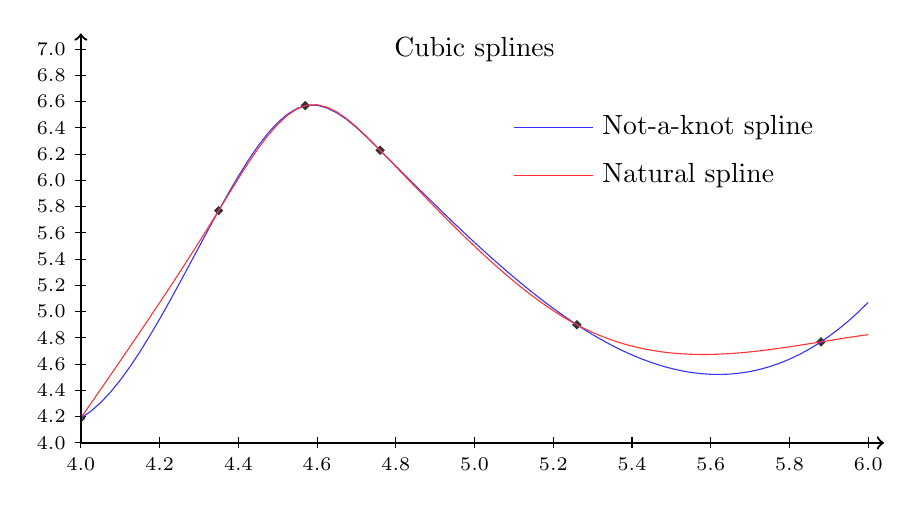
\begin{tikzpicture}
\draw (0.0,0cm + 2pt) -- (0.0, 0cm -2pt) node[below] {\scriptsize{\num[round-mode=places,round-precision=1]{4.0}}};
\draw (0.99999905,0cm + 2pt) -- (0.99999905, 0cm -2pt) node[below] {\scriptsize{\num[round-mode=places,round-precision=1]{4.2}}};
\draw (2.0000005,0cm + 2pt) -- (2.0000005, 0cm -2pt) node[below] {\scriptsize{\num[round-mode=places,round-precision=1]{4.4}}};
\draw (2.9999995,0cm + 2pt) -- (2.9999995, 0cm -2pt) node[below] {\scriptsize{\num[round-mode=places,round-precision=1]{4.6}}};
\draw (4.000001,0cm + 2pt) -- (4.000001, 0cm -2pt) node[below] {\scriptsize{\num[round-mode=places,round-precision=1]{4.8}}};
\draw (5.0,0cm + 2pt) -- (5.0, 0cm -2pt) node[below] {\scriptsize{\num[round-mode=places,round-precision=1]{5.0}}};
\draw (5.999999,0cm + 2pt) -- (5.999999, 0cm -2pt) node[below] {\scriptsize{\num[round-mode=places,round-precision=1]{5.2}}};
\draw (7.0000005,0cm + 2pt) -- (7.0000005, 0cm -2pt) node[below] {\scriptsize{\num[round-mode=places,round-precision=1]{5.4}}};
\draw (7.9999995,0cm + 2pt) -- (7.9999995, 0cm -2pt) node[below] {\scriptsize{\num[round-mode=places,round-precision=1]{5.6}}};
\draw (9.000001,0cm + 2pt) -- (9.000001, 0cm -2pt) node[below] {\scriptsize{\num[round-mode=places,round-precision=1]{5.8}}};
\draw (10.0,0cm + 2pt) -- (10.0, 0cm -2pt) node[below] {\scriptsize{\num[round-mode=places,round-precision=1]{6.0}}};
\draw (0cm + 2pt,0.    ) -- (0cm-2pt,0.    ) node[left] {\scriptsize{\num[round-mode=places,round-precision=1]{4.0}}};
\draw (0cm + 2pt,0.33333302    ) -- (0cm-2pt,0.33333302    ) node[left] {\scriptsize{\num[round-mode=places,round-precision=1]{4.2}}};
\draw (0cm + 2pt,0.6666668    ) -- (0cm-2pt,0.6666668    ) node[left] {\scriptsize{\num[round-mode=places,round-precision=1]{4.4}}};
\draw (0cm + 2pt,0.9999998    ) -- (0cm-2pt,0.9999998    ) node[left] {\scriptsize{\num[round-mode=places,round-precision=1]{4.6}}};
\draw (0cm + 2pt,1.3333336    ) -- (0cm-2pt,1.3333336    ) node[left] {\scriptsize{\num[round-mode=places,round-precision=1]{4.8}}};
\draw (0cm + 2pt,1.6666666    ) -- (0cm-2pt,1.6666666    ) node[left] {\scriptsize{\num[round-mode=places,round-precision=1]{5.0}}};
\draw (0cm + 2pt,1.9999996    ) -- (0cm-2pt,1.9999996    ) node[left] {\scriptsize{\num[round-mode=places,round-precision=1]{5.2}}};
\draw (0cm + 2pt,2.3333335    ) -- (0cm-2pt,2.3333335    ) node[left] {\scriptsize{\num[round-mode=places,round-precision=1]{5.4}}};
\draw (0cm + 2pt,2.6666665    ) -- (0cm-2pt,2.6666665    ) node[left] {\scriptsize{\num[round-mode=places,round-precision=1]{5.6}}};
\draw (0cm + 2pt,3.0000002    ) -- (0cm-2pt,3.0000002    ) node[left] {\scriptsize{\num[round-mode=places,round-precision=1]{5.8}}};
\draw (0cm + 2pt,3.3333333    ) -- (0cm-2pt,3.3333333    ) node[left] {\scriptsize{\num[round-mode=places,round-precision=1]{6.0}}};
\draw (0cm + 2pt,3.6666663    ) -- (0cm-2pt,3.6666663    ) node[left] {\scriptsize{\num[round-mode=places,round-precision=1]{6.2}}};
\draw (0cm + 2pt,4.    ) -- (0cm-2pt,4.    ) node[left] {\scriptsize{\num[round-mode=places,round-precision=1]{6.4}}};
\draw (0cm + 2pt,4.333334    ) -- (0cm-2pt,4.333334    ) node[left] {\scriptsize{\num[round-mode=places,round-precision=1]{6.6000004}}};
\draw (0cm + 2pt,4.666667    ) -- (0cm-2pt,4.666667    ) node[left] {\scriptsize{\num[round-mode=places,round-precision=1]{6.8}}};
\draw (0cm + 2pt,5.    ) -- (0cm-2pt,5.    ) node[left] {\scriptsize{\num[round-mode=places,round-precision=1]{7.0}}};
\node[] at (5.0,5.0) {Cubic splines};
\begin{scope}[]
\clip (0,0) rectangle (10,5);
\node at (0.0,0.316666654083465) [draw=black!80,fill=black!80,diamond,inner sep=0pt,minimum width =3pt,minimum height=3pt] {}; 
\node at (1.7499999739229666,2.949999882777536) [draw=black!80,fill=black!80,diamond,inner sep=0pt,minimum width =3pt,minimum height=3pt] {}; 
\node at (2.8499999575316926,4.283333163128966) [draw=black!80,fill=black!80,diamond,inner sep=0pt,minimum width =3pt,minimum height=3pt] {}; 
\node at (3.799999943375587,3.716666518979609) [draw=black!80,fill=black!80,diamond,inner sep=0pt,minimum width =3pt,minimum height=3pt] {}; 
\node at (6.299999906122685,1.4999999403953581) [draw=black!80,fill=black!80,diamond,inner sep=0pt,minimum width =3pt,minimum height=3pt] {}; 
\node at (9.399999859929085,1.2833332823382497) [draw=black!80,fill=black!80,diamond,inner sep=0pt,minimum width =3pt,minimum height=3pt] {}; 
\begin{scope}[blue!80]
\draw[] (-2.4999999627470975,7.7943914926862305) -- (-2.374999964609743,6.85271188831033);
\draw[] (-2.374999964609743,6.85271188831033) -- (-2.2499999664723886,5.985369091033453);
\draw[] (-2.2499999664723886,5.985369091033453) -- (-2.124999968335032,5.189934920066197);
\draw[] (-2.124999968335032,5.189934920066197) -- (-1.9999999701976776,4.4639811946192065);
\draw[] (-1.9999999701976776,4.4639811946192065) -- (-1.8749999720603232,3.8050797339030833);
\draw[] (-1.8749999720603232,3.8050797339030833) -- (-1.7499999739229688,3.2108023571284394);
\draw[] (-1.7499999739229688,3.2108023571284394) -- (-1.6249999757856144,2.6787208835058913);
\draw[] (-1.6249999757856144,2.6787208835058913) -- (-1.4999999776482578,2.206407132246049);
\draw[] (-1.4999999776482578,2.206407132246049) -- (-1.3749999795109031,1.7914329225595402);
\draw[] (-1.3749999795109031,1.7914329225595402) -- (-1.2499999813735487,1.431370073656974);
\draw[] (-1.2499999813735487,1.431370073656974) -- (-1.1249999832361943,1.1237904047489642);
\draw[] (-1.1249999832361943,1.1237904047489642) -- (-0.9999999850988399,0.8662657350461275);
\draw[] (-0.9999999850988399,0.8662657350461275) -- (-0.8749999869614833,0.6563678837590736);
\draw[] (-0.8749999869614833,0.6563678837590736) -- (-0.7499999888241289,0.49166867009842874);
\draw[] (-0.7499999888241289,0.49166867009842874) -- (-0.6249999906867744,0.36973991327480216);
\draw[] (-0.6249999906867744,0.36973991327480216) -- (-0.49999999254941996,0.2881534324988066);
\draw[] (-0.49999999254941996,0.2881534324988066) -- (-0.3749999944120655,0.24448104698106043);
\draw[] (-0.3749999944120655,0.24448104698106043) -- (-0.24999999627470887,0.23629457593217776);
\draw[] (-0.24999999627470887,0.23629457593217776) -- (-0.12499999813735443,0.26116583856277414);
\draw[] (-0.12499999813735443,0.26116583856277414) -- (0.0,0.316666654083465);
\draw[] (0.0,0.316666654083465) -- (0.12499999813735665,0.4003688417048675);
\draw[] (0.12499999813735665,0.4003688417048675) -- (0.24999999627470887,0.5098442206375896);
\draw[] (0.24999999627470887,0.5098442206375896) -- (0.3749999944120655,0.6426646100922557);
\draw[] (0.3749999944120655,0.6426646100922557) -- (0.49999999254941774,0.7964018292794712);
\draw[] (0.49999999254941774,0.7964018292794712) -- (0.6249999906867744,0.9686276974098632);
\draw[] (0.6249999906867744,0.9686276974098632) -- (0.749999988824131,1.1569140336940429);
\draw[] (0.749999988824131,1.1569140336940429) -- (0.8749999869614833,1.358832657342614);
\draw[] (0.8749999869614833,1.358832657342614) -- (0.9999999850988399,1.5719553875662082);
\draw[] (0.9999999850988399,1.5719553875662082) -- (1.124999983236192,1.793854043575428);
\draw[] (1.124999983236192,1.793854043575428) -- (1.2499999813735487,2.0221004445808974);
\draw[] (1.2499999813735487,2.0221004445808974) -- (1.3749999795109054,2.2542664097932303);
\draw[] (1.3749999795109054,2.2542664097932303) -- (1.4999999776482578,2.487923758423034);
\draw[] (1.4999999776482578,2.487923758423034) -- (1.6249999757856144,2.7206443096809374);
\draw[] (1.6249999757856144,2.7206443096809374) -- (1.7499999739229666,2.9499998827775373);
\draw[] (1.7499999739229666,2.9499998827775373) -- (1.8749999720603232,3.1733231579063315);
\draw[] (1.8749999720603232,3.1733231579063315) -- (1.9999999701976798,3.386990259192244);
\draw[] (1.9999999701976798,3.386990259192244) -- (2.124999968335032,3.5871381717430655);
\draw[] (2.124999968335032,3.5871381717430655) -- (2.2499999664723886,3.7699038806666065);
\draw[] (2.2499999664723886,3.7699038806666065) -- (2.374999964609741,3.931424371070651);
\draw[] (2.374999964609741,3.931424371070651) -- (2.4999999627470975,4.06783662806301);
\draw[] (2.4999999627470975,4.06783662806301) -- (2.624999960884454,4.17527763675147);
\draw[] (2.624999960884454,4.17527763675147) -- (2.7499999590218063,4.24988438224383);
\draw[] (2.7499999590218063,4.24988438224383) -- (2.874999957159163,4.287805970399012);
\draw[] (2.874999957159163,4.287805970399012) -- (2.9999999552965155,4.287761106314666);
\draw[] (2.9999999552965155,4.287761106314666) -- (3.124999953433872,4.254201610371051);
\draw[] (3.124999953433872,4.254201610371051) -- (3.249999951571229,4.192355031020499);
\draw[] (3.249999951571229,4.192355031020499) -- (3.374999949708581,4.1074489167153505);
\draw[] (3.374999949708581,4.1074489167153505) -- (3.4999999478459376,4.004710815907926);
\draw[] (3.4999999478459376,4.004710815907926) -- (3.62499994598329,3.88936827705057);
\draw[] (3.62499994598329,3.88936827705057) -- (3.7499999441206464,3.766648848595603);
\draw[] (3.7499999441206464,3.766648848595603) -- (3.874999942258003,3.641599909911412);
\draw[] (3.874999942258003,3.641599909911412) -- (3.9999999403953552,3.5165729770361955);
\draw[] (3.9999999403953552,3.5165729770361955) -- (4.124999938532712,3.3918442850782133);
\draw[] (4.124999938532712,3.3918442850782133) -- (4.249999936670064,3.2676366857134576);
\draw[] (4.249999936670064,3.2676366857134576) -- (4.374999934807421,3.144173030617912);
\draw[] (4.374999934807421,3.144173030617912) -- (4.499999932944777,3.021676171467562);
\draw[] (4.499999932944777,3.021676171467562) -- (4.6249999310821295,2.9003689599384015);
\draw[] (4.6249999310821295,2.9003689599384015) -- (4.749999929219486,2.7804742477064077);
\draw[] (4.749999929219486,2.7804742477064077) -- (4.874999927356838,2.6622148864475754);
\draw[] (4.874999927356838,2.6622148864475754) -- (4.999999925494195,2.545813727837884);
\draw[] (4.999999925494195,2.545813727837884) -- (5.1249999236315515,2.4314936235533224);
\draw[] (5.1249999236315515,2.4314936235533224) -- (5.249999921768904,2.3194774252698838);
\draw[] (5.249999921768904,2.3194774252698838) -- (5.37499991990626,2.2099879846635475);
\draw[] (5.37499991990626,2.2099879846635475) -- (5.4999999180436125,2.103248153410304);
\draw[] (5.4999999180436125,2.103248153410304) -- (5.624999916180969,1.9994807831861359);
\draw[] (5.624999916180969,1.9994807831861359) -- (5.749999914318326,1.8989087256670316);
\draw[] (5.749999914318326,1.8989087256670316) -- (5.874999912455678,1.8017548325289818);
\draw[] (5.874999912455678,1.8017548325289818) -- (5.999999910593035,1.708241955447969);
\draw[] (5.999999910593035,1.708241955447969) -- (6.124999908730388,1.6185929460999828);
\draw[] (6.124999908730388,1.6185929460999828) -- (6.249999906867744,1.533030656161004);
\draw[] (6.249999906867744,1.533030656161004) -- (6.374999905005101,1.451776384534055);
\draw[] (6.374999905005101,1.451776384534055) -- (6.499999903142453,1.3750281960377477);
\draw[] (6.499999903142453,1.3750281960377477) -- (6.62499990127981,1.3029662698464899);
\draw[] (6.62499990127981,1.3029662698464899) -- (6.749999899417162,1.2357703250538243);
\draw[] (6.749999899417162,1.2357703250538243) -- (6.874999897554519,1.173620080753285);
\draw[] (6.874999897554519,1.173620080753285) -- (6.999999895691875,1.116695256038412);
\draw[] (6.999999895691875,1.116695256038412) -- (7.124999893829227,1.0651755700027439);
\draw[] (7.124999893829227,1.0651755700027439) -- (7.249999891966584,1.0192407417398162);
\draw[] (7.249999891966584,1.0192407417398162) -- (7.374999890103936,0.9790704903431704);
\draw[] (7.374999890103936,0.9790704903431704) -- (7.499999888241293,0.944844534906336);
\draw[] (7.499999888241293,0.944844534906336) -- (7.6249998863786494,0.9167425945228603);
\draw[] (7.6249998863786494,0.9167425945228603) -- (7.749999884516006,0.8949443882862762);
\draw[] (7.749999884516006,0.8949443882862762) -- (7.874999882653358,0.879629635290119);
\draw[] (7.874999882653358,0.879629635290119) -- (7.9999998807907104,0.8709780546279331);
\draw[] (7.9999998807907104,0.8709780546279331) -- (8.124999878928067,0.8691693653932512);
\draw[] (8.124999878928067,0.8691693653932512) -- (8.249999877065424,0.8743832866796089);
\draw[] (8.249999877065424,0.8743832866796089) -- (8.37499987520278,0.8867995375805503);
\draw[] (8.37499987520278,0.8867995375805503) -- (8.499999873340133,0.9065978371896083);
\draw[] (8.499999873340133,0.9065978371896083) -- (8.624999871477485,0.9339579046003212);
\draw[] (8.624999871477485,0.9339579046003212) -- (8.749999869614841,0.9690594589062291);
\draw[] (8.749999869614841,0.9690594589062291) -- (8.874999867752198,1.0120822192008692);
\draw[] (8.874999867752198,1.0120822192008692) -- (8.999999865889555,1.0632059045777764);
\draw[] (8.999999865889555,1.0632059045777764) -- (9.124999864026908,1.12261023413049);
\draw[] (9.124999864026908,1.12261023413049) -- (9.249999862164259,1.190474926952545);
\draw[] (9.249999862164259,1.190474926952545) -- (9.374999860301616,1.2669797021374845);
\draw[] (9.374999860301616,1.2669797021374845) -- (9.499999858438972,1.3523042787788442);
\draw[] (9.499999858438972,1.3523042787788442) -- (9.624999856576329,1.4466283759701621);
\draw[] (9.624999856576329,1.4466283759701621) -- (9.749999854713682,1.5501317128049699);
\draw[] (9.749999854713682,1.5501317128049699) -- (9.874999852851033,1.6629940083768073);
\draw[] (9.874999852851033,1.6629940083768073) -- (9.99999985098839,1.7853949817792232);
\end{scope}
\begin{scope}[red!80]
\draw[] (-2.4999999627470975,-3.605941027545164) -- (-2.374999964609743,-3.38062413015895);
\draw[] (-2.374999964609743,-3.38062413015895) -- (-2.2499999664723886,-3.159797465588856);
\draw[] (-2.2499999664723886,-3.159797465588856) -- (-2.124999968335032,-2.943224705791926);
\draw[] (-2.124999968335032,-2.943224705791926) -- (-1.9999999701976776,-2.730669522725212);
\draw[] (-1.9999999701976776,-2.730669522725212) -- (-1.8749999720603232,-2.5218955883457586);
\draw[] (-1.8749999720603232,-2.5218955883457586) -- (-1.7499999739229688,-2.3166665746106103);
\draw[] (-1.7499999739229688,-2.3166665746106103) -- (-1.6249999757856144,-2.114746153476813);
\draw[] (-1.6249999757856144,-2.114746153476813) -- (-1.4999999776482578,-1.9158979969014112);
\draw[] (-1.4999999776482578,-1.9158979969014112) -- (-1.3749999795109031,-1.7198857768414577);
\draw[] (-1.3749999795109031,-1.7198857768414577) -- (-1.2499999813735487,-1.526473165253995);
\draw[] (-1.2499999813735487,-1.526473165253995) -- (-1.1249999832361943,-1.3354238340960685);
\draw[] (-1.1249999832361943,-1.3354238340960685) -- (-0.9999999850988399,-1.1465014553247257);
\draw[] (-0.9999999850988399,-1.1465014553247257) -- (-0.8749999869614833,-0.95946970089701);
\draw[] (-0.8749999869614833,-0.95946970089701) -- (-0.7499999888241289,-0.7740922427699727);
\draw[] (-0.7499999888241289,-0.7740922427699727) -- (-0.6249999906867744,-0.5901327529006577);
\draw[] (-0.6249999906867744,-0.5901327529006577) -- (-0.49999999254941996,-0.4073549032461111);
\draw[] (-0.49999999254941996,-0.4073549032461111) -- (-0.3749999944120655,-0.2255223657633807);
\draw[] (-0.3749999944120655,-0.2255223657633807) -- (-0.24999999627470887,-0.04439881240950658);
\draw[] (-0.24999999627470887,-0.04439881240950658) -- (-0.12499999813735443,0.1362520848584554);
\draw[] (-0.12499999813735443,0.1362520848584554) -- (0.0,0.316666654083465);
\draw[] (0.0,0.316666654083465) -- (0.12499999813735665,0.4970812233084776);
\draw[] (0.12499999813735665,0.4970812233084776) -- (0.24999999627470887,0.677732120576436);
\draw[] (0.24999999627470887,0.677732120576436) -- (0.3749999944120655,0.8588556739303093);
\draw[] (0.3749999944120655,0.8588556739303093) -- (0.49999999254941774,1.040688211413039);
\draw[] (0.49999999254941774,1.040688211413039) -- (0.6249999906867744,1.2234660610675885);
\draw[] (0.6249999906867744,1.2234660610675885) -- (0.749999988824131,1.4074255509369065);
\draw[] (0.749999988824131,1.4074255509369065) -- (0.8749999869614833,1.5928030090639387);
\draw[] (0.8749999869614833,1.5928030090639387) -- (0.9999999850988399,1.7798347634916558);
\draw[] (0.9999999850988399,1.7798347634916558) -- (1.124999983236192,1.9687571422629948);
\draw[] (1.124999983236192,1.9687571422629948) -- (1.2499999813735487,2.159806473420925);
\draw[] (1.2499999813735487,2.159806473420925) -- (1.3749999795109054,2.353219085008392);
\draw[] (1.3749999795109054,2.353219085008392) -- (1.4999999776482578,2.5492313050683406);
\draw[] (1.4999999776482578,2.5492313050683406) -- (1.6249999757856144,2.748079461643744);
\draw[] (1.6249999757856144,2.748079461643744) -- (1.7499999739229666,2.9499998827775373);
\draw[] (1.7499999739229666,2.9499998827775373) -- (1.8749999720603232,3.154329772046608);
\draw[] (1.8749999720603232,3.154329772046608) -- (1.9999999701976798,3.356809835163513);
\draw[] (1.9999999701976798,3.356809835163513) -- (2.124999968335032,3.552281653374717);
\draw[] (2.124999968335032,3.552281653374717) -- (2.2499999664723886,3.735586807926718);
\draw[] (2.2499999664723886,3.735586807926718) -- (2.374999964609741,3.9015668800659786);
\draw[] (2.374999964609741,3.9015668800659786) -- (2.4999999627470975,4.045063451038991);
\draw[] (2.4999999627470975,4.045063451038991) -- (2.624999960884454,4.160918102092223);
\draw[] (2.624999960884454,4.160918102092223) -- (2.7499999590218063,4.243972414472157);
\draw[] (2.7499999590218063,4.243972414472157) -- (2.874999957159163,4.289082111375187);
\draw[] (2.874999957159163,4.289082111375187) -- (2.9999999552965155,4.294101009379233);
\draw[] (2.9999999552965155,4.294101009379233) -- (3.124999953433872,4.263572067371012);
\draw[] (3.124999953433872,4.263572067371012) -- (3.249999951571229,4.202943329031665);
\draw[] (3.249999951571229,4.202943329031665) -- (3.374999949708581,4.117662838042336);
\draw[] (3.374999949708581,4.117662838042336) -- (3.4999999478459376,4.01317863808416);
\draw[] (3.4999999478459376,4.01317863808416) -- (3.62499994598329,3.8949387728382847);
\draw[] (3.62499994598329,3.8949387728382847) -- (3.7499999441206464,3.768391285985844);
\draw[] (3.7499999441206464,3.768391285985844) -- (3.874999942258003,3.6388018959505035);
\draw[] (3.874999942258003,3.6388018959505035) -- (3.9999999403953552,3.5087081950810326);
\draw[] (3.9999999403953552,3.5087081950810326) -- (4.124999938532712,3.3785476588715095);
\draw[] (4.124999938532712,3.3785476588715095) -- (4.249999936670064,3.248703740517511);
\draw[] (4.249999936670064,3.248703740517511) -- (4.374999934807421,3.1195598932146047);
\draw[] (4.374999934807421,3.1195598932146047) -- (4.499999932944777,2.9914995701583624);
\draw[] (4.499999932944777,2.9914995701583624) -- (4.6249999310821295,2.864906224544363);
\draw[] (4.6249999310821295,2.864906224544363) -- (4.749999929219486,2.740163309568167);
\draw[] (4.749999929219486,2.740163309568167) -- (4.874999927356838,2.617654278425355);
\draw[] (4.874999927356838,2.617654278425355) -- (4.999999925494195,2.497762584311492);
\draw[] (4.999999925494195,2.497762584311492) -- (5.1249999236315515,2.380871680422152);
\draw[] (5.1249999236315515,2.380871680422152) -- (5.249999921768904,2.267365019952912);
\draw[] (5.249999921768904,2.267365019952912) -- (5.37499991990626,2.157626056099335);
\draw[] (5.37499991990626,2.157626056099335) -- (5.4999999180436125,2.0520382420570016);
\draw[] (5.4999999180436125,2.0520382420570016) -- (5.624999916180969,1.9509850310214718);
\draw[] (5.624999916180969,1.9509850310214718) -- (5.749999914318326,1.8548498761883265);
\draw[] (5.749999914318326,1.8548498761883265) -- (5.874999912455678,1.764016230753138);
\draw[] (5.874999912455678,1.764016230753138) -- (5.999999910593035,1.6788675479114719);
\draw[] (5.999999910593035,1.6788675479114719) -- (6.124999908730388,1.5997872808589044);
\draw[] (6.124999908730388,1.5997872808589044) -- (6.249999906867744,1.5271588827910019);
\draw[] (6.249999906867744,1.5271588827910019) -- (6.374999905005101,1.4613418576961836);
\draw[] (6.374999905005101,1.4613418576961836) -- (6.499999903142453,1.4023373584631706);
\draw[] (6.499999903142453,1.4023373584631706) -- (6.62499990127981,1.3498706785945276);
\draw[] (6.62499990127981,1.3498706785945276) -- (6.749999899417162,1.3036600155314544);
\draw[] (6.749999899417162,1.3036600155314544) -- (6.874999897554519,1.2634235667151321);
\draw[] (6.874999897554519,1.2634235667151321) -- (6.999999895691875,1.2288795295867583);
\draw[] (6.999999895691875,1.2288795295867583) -- (7.124999893829227,1.1997461015875226);
\draw[] (7.124999893829227,1.1997461015875226) -- (7.249999891966584,1.175741480158612);
\draw[] (7.249999891966584,1.175741480158612) -- (7.374999890103936,1.1565838627412233);
\draw[] (7.374999890103936,1.1565838627412233) -- (7.499999888241293,1.1419914467765409);
\draw[] (7.499999888241293,1.1419914467765409) -- (7.6249998863786494,1.1316824297057606);
\draw[] (7.6249998863786494,1.1316824297057606) -- (7.749999884516006,1.1253750089700705);
\draw[] (7.749999884516006,1.1253750089700705) -- (7.874999882653358,1.1227873820106633);
\draw[] (7.874999882653358,1.1227873820106633) -- (7.9999998807907104,1.1236377462687277);
\draw[] (7.9999998807907104,1.1236377462687277) -- (8.124999878928067,1.127644299185455);
\draw[] (8.124999878928067,1.127644299185455) -- (8.249999877065424,1.1345252382020363);
\draw[] (8.249999877065424,1.1345252382020363) -- (8.37499987520278,1.143998760759663);
\draw[] (8.37499987520278,1.143998760759663) -- (8.499999873340133,1.155783064299525);
\draw[] (8.499999873340133,1.155783064299525) -- (8.624999871477485,1.1695963462628136);
\draw[] (8.624999871477485,1.1695963462628136) -- (8.749999869614841,1.1851568040907217);
\draw[] (8.749999869614841,1.1851568040907217) -- (8.874999867752198,1.2021826352244345);
\draw[] (8.874999867752198,1.2021826352244345) -- (8.999999865889555,1.220392037105148);
\draw[] (8.999999865889555,1.220392037105148) -- (9.124999864026908,1.2395032071740488);
\draw[] (9.124999864026908,1.2395032071740488) -- (9.249999862164259,1.2592343428723314);
\draw[] (9.249999862164259,1.2592343428723314) -- (9.374999860301616,1.2793036416411872);
\draw[] (9.374999860301616,1.2793036416411872) -- (9.499999858438972,1.2994293009218014);
\draw[] (9.499999858438972,1.2994293009218014) -- (9.624999856576329,1.3193295181553697);
\draw[] (9.624999856576329,1.3193295181553697) -- (9.749999854713682,1.3387224907830808);
\draw[] (9.749999854713682,1.3387224907830808) -- (9.874999852851033,1.3573264162461258);
\draw[] (9.874999852851033,1.3573264162461258) -- (9.99999985098839,1.3748594919856976);
\end{scope}
\end{scope}
\draw[blue!80] (5.5,4.0) -- (6.5,4.0);
\node[right,] at (6.5,4.0) {Not-a-knot spline};
\draw[red!80] (5.5,3.4) -- (6.5,3.4);
\node[right,] at (6.5,3.4) {Natural spline};
\draw[thick,->] (0.0,0.0) -- (10.2,0.0);
\draw[thick,->] (0.0,0.0) -- (0.0,5.2);
\end{tikzpicture}
%%% Local Variables: 
%%% mode: latex 
%%% TeX-master: "master" 
%%% End:


  \caption{Comparison of splines with different end point conditions.}
\end{figure}

\begin{figure}[H]
  \centering
  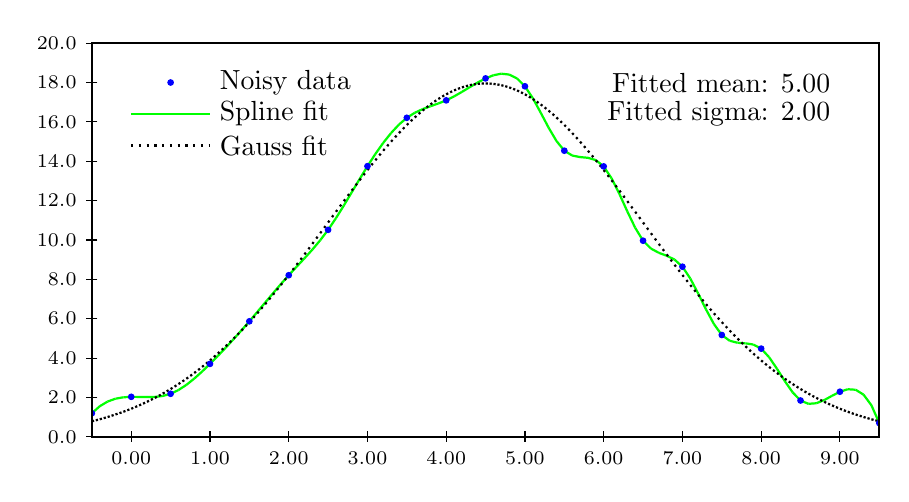
\begin{tikzpicture}
\begin{scope}[]
\clip (0,0) rectangle (10,5);
\begin{scope}[green,thick]
\draw[] (0.0,0.2998554191980206) -- (0.1,0.3886769723521621);
\draw[] (0.1,0.3886769723521621) -- (0.2,0.4483013692841718);
\draw[] (0.2,0.4483013692841718) -- (0.3,0.48433430438467895);
\draw[] (0.3,0.48433430438467895) -- (0.4,0.5023814720443124);
\draw[] (0.4,0.5023814720443124) -- (0.5,0.508048566653701);
\draw[] (0.5,0.508048566653701) -- (0.6,0.506941282603474);
\draw[] (0.6,0.506941282603474) -- (0.7,0.5046653142842601);
\draw[] (0.7,0.5046653142842601) -- (0.8,0.5068263560866882);
\draw[] (0.8,0.5068263560866882) -- (0.9,0.5190301024013876);
\draw[] (0.9,0.5190301024013876) -- (1.0,0.5468822476189868);
\draw[] (1.0,0.5468822476189868) -- (1.1,0.5944637212948228);
\draw[] (1.1,0.5944637212948228) -- (1.2,0.6597563936430622);
\draw[] (1.2,0.6597563936430622) -- (1.3,0.7392173700425795);
\draw[] (1.3,0.7392173700425795) -- (1.4,0.8293037558722491);
\draw[] (1.4,0.8293037558722491) -- (1.5,0.9264726565109458);
\draw[] (1.5,0.9264726565109458) -- (1.6,1.0277622403859983);
\draw[] (1.6,1.0277622403859983) -- (1.7,1.1325349281185535);
\draw[] (1.7,1.1325349281185535) -- (1.8,1.2407342033782138);
\draw[] (1.8,1.2407342033782138) -- (1.9,1.3523035498345806);
\draw[] (1.9,1.3523035498345806) -- (2.0,1.4671864511572559);
\draw[] (2.0,1.4671864511572559) -- (2.1,1.5850318885919035);
\draw[] (2.1,1.5850318885919035) -- (2.2,1.7043108336884367);
\draw[] (2.2,1.7043108336884367) -- (2.3,1.8231997555728292);
\draw[] (2.3,1.8231997555728292) -- (2.4,1.9398751233710578);
\draw[] (2.4,1.9398751233710578) -- (2.5,2.052513406209097);
\draw[] (2.5,2.052513406209097) -- (2.6,2.1603895447518);
\draw[] (2.6,2.1603895447518) -- (2.7,2.2671723658195386);
\draw[] (2.7,2.2671723658195386) -- (2.8,2.37762916777156);
\draw[] (2.8,2.37762916777156) -- (2.9,2.496527248967116);
\draw[] (2.9,2.496527248967116) -- (3.0,2.6286339077654537);
\draw[] (3.0,2.6286339077654537) -- (3.1,2.7769838678261562);
\draw[] (3.1,2.7769838678261562) -- (3.2,2.937681554010137);
\draw[] (3.2,2.937681554010137) -- (3.3,3.1050988164786424);
\draw[] (3.3,3.1050988164786424) -- (3.4,3.2736075053929206);
\draw[] (3.4,3.2736075053929206) -- (3.5,3.437579470914217);
\draw[] (3.5,3.437579470914217) -- (3.6,3.5918608991118726);
\draw[] (3.6,3.5918608991118726) -- (3.7,3.7331953196876033);
\draw[] (3.7,3.7331953196876033) -- (3.8,3.8588005982512175);
\draw[] (3.8,3.8588005982512175) -- (3.9,3.965894600412527);
\draw[] (3.9,3.965894600412527) -- (4.0,4.051695191781341);
\draw[] (4.0,4.051695191781341) -- (4.1,4.115095756069382);
\draw[] (4.1,4.115095756069382) -- (4.2,4.161691749396038);
\draw[] (4.2,4.161691749396038) -- (4.3,4.198754145982606);
\draw[] (4.3,4.198754145982606) -- (4.4,4.233553920050386);
\draw[] (4.4,4.233553920050386) -- (4.5,4.273362045820676);
\draw[] (4.5,4.273362045820676) -- (4.6,4.3234520701688135);
\draw[] (4.6,4.3234520701688135) -- (4.7,4.381107830586282);
\draw[] (4.7,4.381107830586282) -- (4.8,4.441615737218599);
\draw[] (4.8,4.441615737218599) -- (4.9,4.500262200211288);
\draw[] (4.9,4.500262200211288) -- (5.0,4.552333629709862);
\draw[] (5.0,4.552333629709862) -- (5.1,4.59233776594064);
\draw[] (5.1,4.59233776594064) -- (5.2,4.611667669453102);
\draw[] (5.2,4.611667669453102) -- (5.3,4.600937730877521);
\draw[] (5.3,4.600937730877521) -- (5.4,4.550762340844171);
\draw[] (5.4,4.550762340844171) -- (5.5,4.45175588998333);
\draw[] (5.5,4.45175588998333) -- (5.6,4.300437582389341);
\draw[] (5.6,4.300437582389341) -- (5.7,4.116945876012824);
\draw[] (5.7,4.116945876012824) -- (5.8,3.9273240422684816);
\draw[] (5.8,3.9273240422684816) -- (5.9,3.7576153525710008);
\draw[] (5.9,3.7576153525710008) -- (6.0,3.633863078335081);
\draw[] (6.0,3.633863078335081) -- (6.1,3.572659679395789);
\draw[] (6.1,3.572659679395789) -- (6.2,3.5527943692696895);
\draw[] (6.2,3.5527943692696895) -- (6.3,3.543605549893723);
\draw[] (6.3,3.543605549893723) -- (6.4,3.5144316232048283);
\draw[] (6.4,3.5144316232048283) -- (6.5,3.4346109911399463);
\draw[] (6.5,3.4346109911399463) -- (6.6,3.2837879915385906);
\draw[] (6.6,3.2837879915385906) -- (6.7,3.082830705850571);
\draw[] (6.7,3.082830705850571) -- (6.8,2.862913151428279);
\draw[] (6.8,2.862913151428279) -- (6.9,2.655209345624097);
\draw[] (6.9,2.655209345624097) -- (7.0,2.490893305790417);
\draw[] (7.0,2.490893305790417) -- (7.1,2.3911350529230266);
\draw[] (7.1,2.3911350529230266) -- (7.2,2.337088622591336);
\draw[] (7.2,2.337088622591336) -- (7.3,2.299904054008158);
\draw[] (7.3,2.299904054008158) -- (7.4,2.2507313863863057);
\draw[] (7.4,2.2507313863863057) -- (7.5,2.1607206589385934);
\draw[] (7.5,2.1607206589385934) -- (7.6,2.0106625992444567);
\draw[] (7.6,2.0106625992444567) -- (7.7,1.8199106883498228);
\draw[] (7.7,1.8199106883498228) -- (7.8,1.6174590956672459);
\draw[] (7.8,1.6174590956672459) -- (7.9,1.4323019906092747);
\draw[] (7.9,1.4323019906092747) -- (8.0,1.293433542588464);
\draw[] (8.0,1.293433542588464) -- (8.1,1.220344741560056);
\draw[] (8.1,1.220344741560056) -- (8.2,1.1945138596500657);
\draw[] (8.2,1.1945138596500657) -- (8.3,1.1879159895272018);
\draw[] (8.3,1.1879159895272018) -- (8.4,1.172526223860172);
\draw[] (8.4,1.172526223860172) -- (8.5,1.1203196553176844);
\draw[] (8.5,1.1203196553176844) -- (8.6,1.012354246334453);
\draw[] (8.6,1.012354246334453) -- (8.7,0.8660194384092178);
\draw[] (8.7,0.8660194384092178) -- (8.8,0.707787542806721);
\draw[] (8.8,0.707787542806721) -- (8.9,0.5641308707917143);
\draw[] (8.9,0.5641308707917143) -- (9.0,0.46152173362894033);
\draw[] (9.0,0.46152173362894033) -- (9.1,0.41909065427502007);
\draw[] (9.1,0.41909065427502007) -- (9.2,0.4266010024540752);
\draw[] (9.2,0.4266010024540752) -- (9.3,0.46647435958210365);
\draw[] (9.3,0.46647435958210365) -- (9.4,0.5211323070751007);
\draw[] (9.4,0.5211323070751007) -- (9.5,0.5729964263490639);
\draw[] (9.5,0.5729964263490639) -- (9.6,0.6044882988199899);
\draw[] (9.6,0.6044882988199899) -- (9.7,0.5980295059038759);
\draw[] (9.7,0.5980295059038759) -- (9.8,0.5360416290167176);
\draw[] (9.8,0.5360416290167176) -- (9.9,0.4009462495745133);
\draw[] (9.9,0.4009462495745133) -- (10.0,0.1751649489932598);
\end{scope}
\begin{scope}[dotted, thick]
\draw[] (0.0,0.19719338055255084) -- (0.05,0.20984567391293701);
\draw[] (0.05,0.20984567391293701) -- (0.1,0.2231702369075935);
\draw[] (0.1,0.2231702369075935) -- (0.15,0.23719257748861314);
\draw[] (0.15,0.23719257748861314) -- (0.2,0.25193846581686985);
\draw[] (0.2,0.25193846581686985) -- (0.25,0.26743388433641285);
\draw[] (0.25,0.26743388433641285) -- (0.3,0.2837049740458145);
\draw[] (0.3,0.2837049740458145) -- (0.35,0.3007779769376655);
\draw[] (0.35,0.3007779769376655) -- (0.4,0.3186791745928813);
\draw[] (0.4,0.3186791745928813) -- (0.45,0.33743482293299765);
\draw[] (0.45,0.33743482293299765) -- (0.5,0.3570710831511164);
\draw[] (0.5,0.3570710831511164) -- (0.55,0.37761394886060007);
\draw[] (0.55,0.37761394886060007) -- (0.6,0.3990891695199511);
\draw[] (0.6,0.3990891695199511) -- (0.65,0.42152217021247246);
\draw[] (0.65,0.42152217021247246) -- (0.7,0.444937967880252);
\draw[] (0.7,0.444937967880252) -- (0.75,0.46936108413364097);
\draw[] (0.75,0.46936108413364097) -- (0.8,0.49481545477963207);
\draw[] (0.8,0.49481545477963207) -- (0.85,0.5213243362352994);
\draw[] (0.85,0.5213243362352994) -- (0.9,0.5489102090156216);
\draw[] (0.9,0.5489102090156216) -- (0.95,0.5775946785084662);
\draw[] (0.95,0.5775946785084662) -- (1.0,0.60739837327317);
\draw[] (1.0,0.60739837327317) -- (1.05,0.6383408411228194);
\draw[] (1.05,0.6383408411228194) -- (1.1,0.6704404432739747);
\draw[] (1.1,0.6704404432739747) -- (1.15,0.7037142468709632);
\draw[] (1.15,0.7037142468709632) -- (1.2,0.738177916214895);
\draw[] (1.2,0.738177916214895) -- (1.25,0.7738456030500619);
\draw[] (1.25,0.7738456030500619) -- (1.3,0.8107298362822254);
\draw[] (1.3,0.8107298362822254) -- (1.35,0.8488414115242828);
\draw[] (1.35,0.8488414115242828) -- (1.4,0.8881892808848224);
\draw[] (1.4,0.8881892808848224) -- (1.45,0.9287804434339139);
\draw[] (1.45,0.9287804434339139) -- (1.5,0.9706198367980078);
\draw[] (1.5,0.9706198367980078) -- (1.55,1.0137102303518524);
\draw[] (1.55,1.0137102303518524) -- (1.6,1.0580521204897222);
\draw[] (1.6,1.0580521204897222) -- (1.65,1.1036436284708402);
\draw[] (1.65,1.1036436284708402) -- (1.7,1.1504804013444883);
\draw[] (1.7,1.1504804013444883) -- (1.75,1.1985555164688135);
\draw[] (1.75,1.1985555164688135) -- (1.8,1.2478593901436028);
\draw[] (1.8,1.2478593901436028) -- (1.85,1.2983796908811616);
\draw[] (1.85,1.2983796908811616) -- (1.9,1.350101257840809);
\draw[] (1.9,1.350101257840809) -- (1.95,1.4030060249512366);
\draw[] (1.95,1.4030060249512366) -- (2.0,1.4570729512409966);
\draw[] (2.0,1.4570729512409966) -- (2.05,1.5122779578906014);
\draw[] (2.05,1.5122779578906014) -- (2.1,1.5685938725100126);
\draw[] (2.1,1.5685938725100126) -- (2.15,1.6259903811327017);
\draw[] (2.15,1.6259903811327017) -- (2.2,1.6844339884018351);
\draw[] (2.2,1.6844339884018351) -- (2.25,1.743887986405502);
\draw[] (2.25,1.743887986405502) -- (2.3,1.8043124325962971);
\draw[] (2.3,1.8043124325962971) -- (2.35,1.865664137205879);
\draw[] (2.35,1.865664137205879) -- (2.4,1.9278966605375325);
\draw[] (2.4,1.9278966605375325) -- (2.45,1.9909603204892214);
\draw[] (2.45,1.9909603204892214) -- (2.5,2.0548022106261956);
\draw[] (2.5,2.0548022106261956) -- (2.55,2.11936622908612);
\draw[] (2.55,2.11936622908612) -- (2.6,2.184593118560845);
\draw[] (2.6,2.184593118560845) -- (2.65,2.250420517557687);
\draw[] (2.65,2.250420517557687) -- (2.7,2.3167830230994166);
\draw[] (2.7,2.3167830230994166) -- (2.75,2.3836122649763207);
\draw[] (2.75,2.3836122649763207) -- (2.8,2.4508369916158963);
\draw[] (2.8,2.4508369916158963) -- (2.85,2.5183831675861494);
\draw[] (2.85,2.5183831675861494) -- (2.9,2.586174082697328);
\draw[] (2.9,2.586174082697328) -- (2.95,2.654130472614525);
\draw[] (2.95,2.654130472614525) -- (3.0,2.722170650840074);
\draw[] (3.0,2.722170650840074) -- (3.05,2.7902106518705065);
\draw[] (3.05,2.7902106518705065) -- (3.1,2.8581643852780934);
\draw[] (3.1,2.8581643852780934) -- (3.15,2.925943800412172);
\draw[] (3.15,2.925943800412172) -- (3.2,2.9934590613607153);
\draw[] (3.2,2.9934590613607153) -- (3.25,3.0606187317583413);
\draw[] (3.25,3.0606187317583413) -- (3.3,3.127329968973441);
\draw[] (3.3,3.127329968973441) -- (3.35,3.193498727154717);
\draw[] (3.35,3.193498727154717) -- (3.4,3.2590299685664195);
\draw[] (3.4,3.2590299685664195) -- (3.45,3.323827882592326);
\draw[] (3.45,3.323827882592326) -- (3.5,3.387796111741297);
\draw[] (3.5,3.387796111741297) -- (3.55,3.450837983942451);
\draw[] (3.55,3.450837983942451) -- (3.6,3.5128567503758203);
\draw[] (3.6,3.5128567503758203) -- (3.65,3.5737558280451784);
\draw[] (3.65,3.5737558280451784) -- (3.7,3.6334390462638013);
\draw[] (3.7,3.6334390462638013) -- (3.75,3.6918108961914897);
\draw[] (3.75,3.6918108961914897) -- (3.8,3.7487767825325204);
\draw[] (3.8,3.7487767825325204) -- (3.85,3.804243276479533);
\draw[] (3.85,3.804243276479533) -- (3.9,3.858118368967853);
\draw[] (3.9,3.858118368967853) -- (3.95,3.910311723288705);
\draw[] (3.95,3.910311723288705) -- (4.0,3.9607349260981626);
\draw[] (4.0,3.9607349260981626) -- (4.05,4.009301735851859);
\draw[] (4.05,4.009301735851859) -- (4.1,4.0559283276933416);
\draw[] (4.1,4.0559283276933416) -- (4.15,4.100533533826755);
\draw[] (4.15,4.100533533826755) -- (4.2,4.143039078412198);
\draw[] (4.2,4.143039078412198) -- (4.25,4.183369806034715);
\draw[] (4.25,4.183369806034715) -- (4.3,4.2214539028153695);
\draw[] (4.3,4.2214539028153695) -- (4.35,4.257223109255291);
\draw[] (4.35,4.257223109255291) -- (4.4,4.290612923930722);
\draw[] (4.4,4.290612923930722) -- (4.45,4.321562797189007);
\draw[] (4.45,4.321562797189007) -- (4.5,4.350016314031885);
\draw[] (4.5,4.350016314031885) -- (4.55,4.375921365413266);
\draw[] (4.55,4.375921365413266) -- (4.6,4.399230307223716);
\draw[] (4.6,4.399230307223716) -- (4.65,4.4199001062828565);
\draw[] (4.65,4.4199001062828565) -- (4.7,4.4378924727135916);
\draw[] (4.7,4.4378924727135916) -- (4.75,4.453173978128275);
\draw[] (4.75,4.453173978128275) -- (4.8,4.465716159116226);
\draw[] (4.8,4.465716159116226) -- (4.85,4.475495605584188);
\draw[] (4.85,4.475495605584188) -- (4.9,4.482494033565941);
\draw[] (4.9,4.482494033565941) -- (4.95,4.486698342184142);
\draw[] (4.95,4.486698342184142) -- (5.0,4.488100654515964);
\draw[] (5.0,4.488100654515964) -- (5.05,4.486698342184142);
\draw[] (5.05,4.486698342184142) -- (5.1,4.482494033565941);
\draw[] (5.1,4.482494033565941) -- (5.15,4.475495605584188);
\draw[] (5.15,4.475495605584188) -- (5.2,4.465716159116226);
\draw[] (5.2,4.465716159116226) -- (5.25,4.453173978128275);
\draw[] (5.25,4.453173978128275) -- (5.3,4.4378924727135916);
\draw[] (5.3,4.4378924727135916) -- (5.35,4.4199001062828565);
\draw[] (5.35,4.4199001062828565) -- (5.4,4.399230307223716);
\draw[] (5.4,4.399230307223716) -- (5.45,4.375921365413266);
\draw[] (5.45,4.375921365413266) -- (5.5,4.350016314031885);
\draw[] (5.5,4.350016314031885) -- (5.55,4.321562797189007);
\draw[] (5.55,4.321562797189007) -- (5.6,4.290612923930722);
\draw[] (5.6,4.290612923930722) -- (5.65,4.257223109255291);
\draw[] (5.65,4.257223109255291) -- (5.7,4.2214539028153695);
\draw[] (5.7,4.2214539028153695) -- (5.75,4.183369806034715);
\draw[] (5.75,4.183369806034715) -- (5.8,4.143039078412198);
\draw[] (5.8,4.143039078412198) -- (5.85,4.100533533826755);
\draw[] (5.85,4.100533533826755) -- (5.9,4.0559283276933416);
\draw[] (5.9,4.0559283276933416) -- (5.95,4.009301735851859);
\draw[] (5.95,4.009301735851859) -- (6.0,3.9607349260981626);
\draw[] (6.0,3.9607349260981626) -- (6.05,3.910311723288705);
\draw[] (6.05,3.910311723288705) -- (6.1,3.8581183689678533);
\draw[] (6.1,3.8581183689678533) -- (6.15,3.8042432764795326);
\draw[] (6.15,3.8042432764795326) -- (6.2,3.7487767825325204);
\draw[] (6.2,3.7487767825325204) -- (6.25,3.6918108961914897);
\draw[] (6.25,3.6918108961914897) -- (6.3,3.6334390462638013);
\draw[] (6.3,3.6334390462638013) -- (6.35,3.573755828045179);
\draw[] (6.35,3.573755828045179) -- (6.4,3.51285675037582);
\draw[] (6.4,3.51285675037582) -- (6.45,3.450837983942451);
\draw[] (6.45,3.450837983942451) -- (6.5,3.387796111741297);
\draw[] (6.5,3.387796111741297) -- (6.55,3.323827882592326);
\draw[] (6.55,3.323827882592326) -- (6.6,3.25902996856642);
\draw[] (6.6,3.25902996856642) -- (6.65,3.1934987271547164);
\draw[] (6.65,3.1934987271547164) -- (6.7,3.127329968973441);
\draw[] (6.7,3.127329968973441) -- (6.75,3.0606187317583413);
\draw[] (6.75,3.0606187317583413) -- (6.8,2.9934590613607153);
\draw[] (6.8,2.9934590613607153) -- (6.85,2.9259438004121723);
\draw[] (6.85,2.9259438004121723) -- (6.9,2.8581643852780925);
\draw[] (6.9,2.8581643852780925) -- (6.95,2.7902106518705065);
\draw[] (6.95,2.7902106518705065) -- (7.0,2.722170650840074);
\draw[] (7.0,2.722170650840074) -- (7.05,2.654130472614525);
\draw[] (7.05,2.654130472614525) -- (7.1,2.5861740826973287);
\draw[] (7.1,2.5861740826973287) -- (7.15,2.5183831675861486);
\draw[] (7.15,2.5183831675861486) -- (7.2,2.4508369916158963);
\draw[] (7.2,2.4508369916158963) -- (7.25,2.3836122649763207);
\draw[] (7.25,2.3836122649763207) -- (7.3,2.3167830230994166);
\draw[] (7.3,2.3167830230994166) -- (7.35,2.2504205175576875);
\draw[] (7.35,2.2504205175576875) -- (7.4,2.1845931185608447);
\draw[] (7.4,2.1845931185608447) -- (7.45,2.11936622908612);
\draw[] (7.45,2.11936622908612) -- (7.5,2.0548022106261956);
\draw[] (7.5,2.0548022106261956) -- (7.55,1.9909603204892214);
\draw[] (7.55,1.9909603204892214) -- (7.6,1.927896660537533);
\draw[] (7.6,1.927896660537533) -- (7.65,1.8656641372058782);
\draw[] (7.65,1.8656641372058782) -- (7.7,1.8043124325962971);
\draw[] (7.7,1.8043124325962971) -- (7.75,1.743887986405502);
\draw[] (7.75,1.743887986405502) -- (7.8,1.6844339884018351);
\draw[] (7.8,1.6844339884018351) -- (7.85,1.6259903811327023);
\draw[] (7.85,1.6259903811327023) -- (7.9,1.5685938725100121);
\draw[] (7.9,1.5685938725100121) -- (7.95,1.5122779578906014);
\draw[] (7.95,1.5122779578906014) -- (8.0,1.4570729512409966);
\draw[] (8.0,1.4570729512409966) -- (8.05,1.4030060249512355);
\draw[] (8.05,1.4030060249512355) -- (8.1,1.3501012578408094);
\draw[] (8.1,1.3501012578408094) -- (8.15,1.298379690881161);
\draw[] (8.15,1.298379690881161) -- (8.2,1.2478593901436035);
\draw[] (8.2,1.2478593901436035) -- (8.25,1.1985555164688135);
\draw[] (8.25,1.1985555164688135) -- (8.3,1.1504804013444876);
\draw[] (8.3,1.1504804013444876) -- (8.35,1.1036436284708406);
\draw[] (8.35,1.1036436284708406) -- (8.4,1.0580521204897217);
\draw[] (8.4,1.0580521204897217) -- (8.45,1.013710230351853);
\draw[] (8.45,1.013710230351853) -- (8.5,0.9706198367980078);
\draw[] (8.5,0.9706198367980078) -- (8.55,0.9287804434339132);
\draw[] (8.55,0.9287804434339132) -- (8.6,0.8881892808848225);
\draw[] (8.6,0.8881892808848225) -- (8.65,0.8488414115242826);
\draw[] (8.65,0.8488414115242826) -- (8.7,0.8107298362822261);
\draw[] (8.7,0.8107298362822261) -- (8.75,0.7738456030500619);
\draw[] (8.75,0.7738456030500619) -- (8.8,0.7381779162148944);
\draw[] (8.8,0.7381779162148944) -- (8.85,0.7037142468709636);
\draw[] (8.85,0.7037142468709636) -- (8.9,0.6704404432739745);
\draw[] (8.9,0.6704404432739745) -- (8.95,0.63834084112282);
\draw[] (8.95,0.63834084112282) -- (9.0,0.60739837327317);
\draw[] (9.0,0.60739837327317) -- (9.05,0.5775946785084658);
\draw[] (9.05,0.5775946785084658) -- (9.1,0.5489102090156216);
\draw[] (9.1,0.5489102090156216) -- (9.15,0.5213243362352994);
\draw[] (9.15,0.5213243362352994) -- (9.2,0.4948154547796325);
\draw[] (9.2,0.4948154547796325) -- (9.25,0.46936108413364097);
\draw[] (9.25,0.46936108413364097) -- (9.3,0.4449379678802516);
\draw[] (9.3,0.4449379678802516) -- (9.35,0.42152217021247246);
\draw[] (9.35,0.42152217021247246) -- (9.4,0.3990891695199511);
\draw[] (9.4,0.3990891695199511) -- (9.45,0.37761394886060046);
\draw[] (9.45,0.37761394886060046) -- (9.5,0.3570710831511164);
\draw[] (9.5,0.3570710831511164) -- (9.55,0.3374348229329973);
\draw[] (9.55,0.3374348229329973) -- (9.6,0.3186791745928813);
\draw[] (9.6,0.3186791745928813) -- (9.65,0.3007779769376655);
\draw[] (9.65,0.3007779769376655) -- (9.7,0.2837049740458149);
\draw[] (9.7,0.2837049740458149) -- (9.75,0.26743388433641285);
\draw[] (9.75,0.26743388433641285) -- (9.8,0.25193846581686963);
\draw[] (9.8,0.25193846581686963) -- (9.85,0.23719257748861314);
\draw[] (9.85,0.23719257748861314) -- (9.9,0.2231702369075935);
\draw[] (9.9,0.2231702369075935) -- (9.95,0.2098456739129372);
\draw[] (9.95,0.2098456739129372) -- (10.0,0.19719338055255084);
\end{scope}
\draw[draw=blue,fill=blue] (0.0,0.2998554191980206) circle(1pt); 
\draw[draw=blue,fill=blue] (0.5,0.5080485666537011) circle(1pt); 
\draw[draw=blue,fill=blue] (1.0,0.5468822476189868) circle(1pt); 
\draw[draw=blue,fill=blue] (1.5,0.9264726565109457) circle(1pt); 
\draw[draw=blue,fill=blue] (2.0,1.4671864511572559) circle(1pt); 
\draw[draw=blue,fill=blue] (2.5,2.052513406209097) circle(1pt); 
\draw[draw=blue,fill=blue] (3.0,2.6286339077654537) circle(1pt); 
\draw[draw=blue,fill=blue] (3.5,3.437579470914217) circle(1pt); 
\draw[draw=blue,fill=blue] (4.0,4.051695191781341) circle(1pt); 
\draw[draw=blue,fill=blue] (4.5,4.273362045820676) circle(1pt); 
\draw[draw=blue,fill=blue] (5.0,4.552333629709863) circle(1pt); 
\draw[draw=blue,fill=blue] (5.5,4.45175588998333) circle(1pt); 
\draw[draw=blue,fill=blue] (6.0,3.633863078335081) circle(1pt); 
\draw[draw=blue,fill=blue] (6.5,3.4346109911399463) circle(1pt); 
\draw[draw=blue,fill=blue] (7.0,2.490893305790417) circle(1pt); 
\draw[draw=blue,fill=blue] (7.5,2.1607206589385934) circle(1pt); 
\draw[draw=blue,fill=blue] (8.0,1.293433542588464) circle(1pt); 
\draw[draw=blue,fill=blue] (8.5,1.1203196553176844) circle(1pt); 
\draw[draw=blue,fill=blue] (9.0,0.46152173362894033) circle(1pt); 
\draw[draw=blue,fill=blue] (9.5,0.5729964263490638) circle(1pt); 
\draw[draw=blue,fill=blue] (10.0,0.17516494899325974) circle(1pt); 
\end{scope}
\draw (0.5,0cm + 2pt) -- (0.5, 0cm -2pt) node[below] {\scriptsize{\num[round-mode=places,round-precision=2]{0}}};
\draw (1.5,0cm + 2pt) -- (1.5, 0cm -2pt) node[below] {\scriptsize{\num[round-mode=places,round-precision=2]{1}}};
\draw (2.5,0cm + 2pt) -- (2.5, 0cm -2pt) node[below] {\scriptsize{\num[round-mode=places,round-precision=2]{2}}};
\draw (3.5,0cm + 2pt) -- (3.5, 0cm -2pt) node[below] {\scriptsize{\num[round-mode=places,round-precision=2]{3}}};
\draw (4.5,0cm + 2pt) -- (4.5, 0cm -2pt) node[below] {\scriptsize{\num[round-mode=places,round-precision=2]{4}}};
\draw (5.5,0cm + 2pt) -- (5.5, 0cm -2pt) node[below] {\scriptsize{\num[round-mode=places,round-precision=2]{5}}};
\draw (6.5,0cm + 2pt) -- (6.5, 0cm -2pt) node[below] {\scriptsize{\num[round-mode=places,round-precision=2]{6}}};
\draw (7.5,0cm + 2pt) -- (7.5, 0cm -2pt) node[below] {\scriptsize{\num[round-mode=places,round-precision=2]{7}}};
\draw (8.5,0cm + 2pt) -- (8.5, 0cm -2pt) node[below] {\scriptsize{\num[round-mode=places,round-precision=2]{8}}};
\draw (9.5,0cm + 2pt) -- (9.5, 0cm -2pt) node[below] {\scriptsize{\num[round-mode=places,round-precision=2]{9}}};
\draw (0cm + 2pt,0.    ) -- (0cm-2pt,0.    ) node[left] {\scriptsize{\num[round-mode=places,round-precision=1]{0}}};
\draw (0cm + 2pt,0.5    ) -- (0cm-2pt,0.5    ) node[left] {\scriptsize{\num[round-mode=places,round-precision=1]{2}}};
\draw (0cm + 2pt,1.    ) -- (0cm-2pt,1.    ) node[left] {\scriptsize{\num[round-mode=places,round-precision=1]{4}}};
\draw (0cm + 2pt,1.5    ) -- (0cm-2pt,1.5    ) node[left] {\scriptsize{\num[round-mode=places,round-precision=1]{6}}};
\draw (0cm + 2pt,2.    ) -- (0cm-2pt,2.    ) node[left] {\scriptsize{\num[round-mode=places,round-precision=1]{8}}};
\draw (0cm + 2pt,2.5    ) -- (0cm-2pt,2.5    ) node[left] {\scriptsize{\num[round-mode=places,round-precision=1]{10}}};
\draw (0cm + 2pt,3.    ) -- (0cm-2pt,3.    ) node[left] {\scriptsize{\num[round-mode=places,round-precision=1]{12}}};
\draw (0cm + 2pt,3.5    ) -- (0cm-2pt,3.5    ) node[left] {\scriptsize{\num[round-mode=places,round-precision=1]{14}}};
\draw (0cm + 2pt,4.    ) -- (0cm-2pt,4.    ) node[left] {\scriptsize{\num[round-mode=places,round-precision=1]{16}}};
\draw (0cm + 2pt,4.5    ) -- (0cm-2pt,4.5    ) node[left] {\scriptsize{\num[round-mode=places,round-precision=1]{18}}};
\draw (0cm + 2pt,5.    ) -- (0cm-2pt,5.    ) node[left] {\scriptsize{\num[round-mode=places,round-precision=1]{20}}};
\draw[draw=blue,fill=blue] (1.0,4.5) circle(1pt); 
\node[right,] at (1.5,4.5) {Noisy data};
\draw[draw=green,thick] (0.5,4.1) -- (1.5,4.1);
\node[right,] at (1.5,4.1) {Spline fit};
\draw[thick,dotted] (0.5,3.7) -- (1.5,3.7);
\node[right,] at (1.5,3.7) {Gauss fit};
\node[left] at (9.5,4.5) {Fitted mean:  5.00};
\node[left] at (9.5,4.1) {Fitted sigma:  2.00};
\draw[thick] (0,0) rectangle (10,5);
\end{tikzpicture}
%%% Local Variables: 
%%% mode: latex 
%%% TeX-master: "master" 
%%% End:


  \caption{The Gaussian function fitted to a set of noisy measurements}
\end{figure}

\begin{figure}[H]
  \centering
  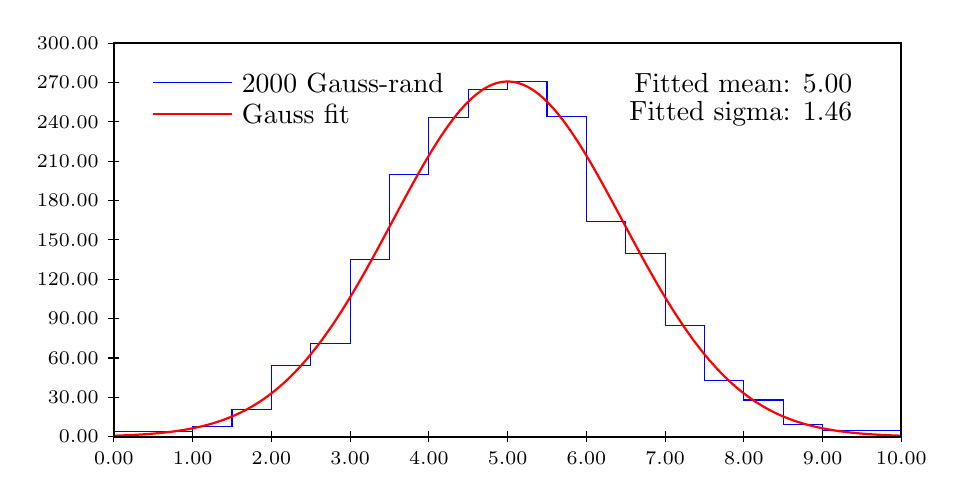
\begin{tikzpicture}[]
\begin{scope}[]
\clip (0.0,0.0) rectangle (10.0,5.0);
\begin{scope}[shift={(0.0,0.0)}]
\pgfsetxvec{\pgfpoint{1.0cm}{0cm}}
\pgfsetyvec{\pgfpoint{0cm}{0.016666668cm}}
\begin{scope}[shift={(0.0,0.0)}]
\begin{scope}[draw=blue]
\pgfpathmoveto{ \pgfpointxy {10.0} {0.0}}
\pgfpathlineto{ \pgfpointxy {10.0} {5.0}}
\pgfpathlineto{ \pgfpointxy {9.5} {5.0}}
\pgfpathlineto{ \pgfpointxy {9.5} {5.0}}
\pgfpathlineto{ \pgfpointxy {9.0} {5.0}}
\pgfpathlineto{ \pgfpointxy {9.0} {9.0}}
\pgfpathlineto{ \pgfpointxy {8.5} {9.0}}
\pgfpathlineto{ \pgfpointxy {8.5} {28.0}}
\pgfpathlineto{ \pgfpointxy {8.0} {28.0}}
\pgfpathlineto{ \pgfpointxy {8.0} {43.0}}
\pgfpathlineto{ \pgfpointxy {7.5} {43.0}}
\pgfpathlineto{ \pgfpointxy {7.5} {85.0}}
\pgfpathlineto{ \pgfpointxy {7.0} {85.0}}
\pgfpathlineto{ \pgfpointxy {7.0} {140.0}}
\pgfpathlineto{ \pgfpointxy {6.5} {140.0}}
\pgfpathlineto{ \pgfpointxy {6.5} {164.0}}
\pgfpathlineto{ \pgfpointxy {6.0} {164.0}}
\pgfpathlineto{ \pgfpointxy {6.0} {244.0}}
\pgfpathlineto{ \pgfpointxy {5.5} {244.0}}
\pgfpathlineto{ \pgfpointxy {5.5} {271.0}}
\pgfpathlineto{ \pgfpointxy {5.0} {271.0}}
\pgfpathlineto{ \pgfpointxy {5.0} {265.0}}
\pgfpathlineto{ \pgfpointxy {4.5} {265.0}}
\pgfpathlineto{ \pgfpointxy {4.5} {243.0}}
\pgfpathlineto{ \pgfpointxy {4.0} {243.0}}
\pgfpathlineto{ \pgfpointxy {4.0} {200.0}}
\pgfpathlineto{ \pgfpointxy {3.5} {200.0}}
\pgfpathlineto{ \pgfpointxy {3.5} {135.0}}
\pgfpathlineto{ \pgfpointxy {3.0} {135.0}}
\pgfpathlineto{ \pgfpointxy {3.0} {71.0}}
\pgfpathlineto{ \pgfpointxy {2.5} {71.0}}
\pgfpathlineto{ \pgfpointxy {2.5} {54.0}}
\pgfpathlineto{ \pgfpointxy {2.0} {54.0}}
\pgfpathlineto{ \pgfpointxy {2.0} {21.0}}
\pgfpathlineto{ \pgfpointxy {1.5} {21.0}}
\pgfpathlineto{ \pgfpointxy {1.5} {8.0}}
\pgfpathlineto{ \pgfpointxy {1.0} {8.0}}
\pgfpathlineto{ \pgfpointxy {1.0} {4.0}}
\pgfpathlineto{ \pgfpointxy {0.5} {4.0}}
\pgfpathlineto{ \pgfpointxy {0.5} {4.0}}
\pgfpathlineto{ \pgfpointxy {0.0} {4.0}}
\pgfpathlineto{ \pgfpointxy {0.0} {0.0}}
\pgfusepath{ stroke, }
\end{scope}
\end{scope}
\pgfsetxvec{\pgfpoint{1cm}{0cm}}
\pgfsetyvec{\pgfpoint{0cm}{1cm}}
\end{scope}
\end{scope}
\node[left] at (9.5,4.5) {Fitted mean:  5.00};
\node[left] at (9.5,4.1) {Fitted sigma:  1.46};
\begin{scope}[]
\clip (0.0,0.0) rectangle (10.0,5.0);
\begin{scope}[shift={(0.0,0.0)}]
\pgfsetxvec{\pgfpoint{1.0cm}{0cm}}
\pgfsetyvec{\pgfpoint{0cm}{0.016666668cm}}
\begin{scope}[shift={(0.0,0.0)}]
\begin{scope}[thick,red]
\pgfpathmoveto{ \pgfpointxy {0.0} {0.785533585190544}}
\pgfpathlineto{ \pgfpointxy {0.05} {0.8823944062104124}}
\pgfpathlineto{ \pgfpointxy {0.1} {0.9900410132316494}}
\pgfpathlineto{ \pgfpointxy {0.15} {1.1095224058046345}}
\pgfpathlineto{ \pgfpointxy {0.2} {1.2419708963422873}}
\pgfpathlineto{ \pgfpointxy {0.25} {1.3886065589283518}}
\pgfpathlineto{ \pgfpointxy {0.3} {1.5507416694118887}}
\pgfpathlineto{ \pgfpointxy {0.35} {1.7297851028337528}}
\pgfpathlineto{ \pgfpointxy {0.4} {1.927246650571349}}
\pgfpathlineto{ \pgfpointxy {0.45} {2.144741215868452}}
\pgfpathlineto{ \pgfpointxy {0.5} {2.383992842671168}}
\pgfpathlineto{ \pgfpointxy {0.55} {2.646838528957892}}
\pgfpathlineto{ \pgfpointxy {0.6} {2.935231772073318}}
\pgfpathlineto{ \pgfpointxy {0.65} {3.251245790000996}}
\pgfpathlineto{ \pgfpointxy {0.7} {3.5970763590868597}}
\pgfpathlineto{ \pgfpointxy {0.75} {3.9750442055123947}}
\pgfpathlineto{ \pgfpointxy {0.8} {4.387596884868998}}
\pgfpathlineto{ \pgfpointxy {0.85} {4.8373100815661525}}
\pgfpathlineto{ \pgfpointxy {0.9} {5.326888257579253}}
\pgfpathlineto{ \pgfpointxy {0.95} {5.859164578274084}}
\pgfpathlineto{ \pgfpointxy {1.0} {6.437100041802212}}
\pgfpathlineto{ \pgfpointxy {1.05} {7.063781737911131}}
\pgfpathlineto{ \pgfpointxy {1.1} {7.742420162024598}}
\pgfpathlineto{ \pgfpointxy {1.15} {8.476345511186555}}
\pgfpathlineto{ \pgfpointxy {1.2} {9.269002889991516}}
\pgfpathlineto{ \pgfpointxy {1.25} {10.12394635700542}}
\pgfpathlineto{ \pgfpointxy {1.3} {11.044831745470251}}
\pgfpathlineto{ \pgfpointxy {1.35} {12.035408196332893}}
\pgfpathlineto{ \pgfpointxy {1.4} {13.099508346888094}}
\pgfpathlineto{ \pgfpointxy {1.45} {14.241037124611898}}
\pgfpathlineto{ \pgfpointxy {1.5} {15.463959103111062}}
\pgfpathlineto{ \pgfpointxy {1.55} {16.77228438554224}}
\pgfpathlineto{ \pgfpointxy {1.6} {18.170052990364315}}
\pgfpathlineto{ \pgfpointxy {1.65} {19.661317724870088}}
\pgfpathlineto{ \pgfpointxy {1.7} {21.250125543575855}}
\pgfpathlineto{ \pgfpointxy {1.75} {22.940497401191028}}
\pgfpathlineto{ \pgfpointxy {1.8} {24.736406623493174}}
\pgfpathlineto{ \pgfpointxy {1.85} {26.64175583392414}}
\pgfpathlineto{ \pgfpointxy {1.9} {28.660352489018294}}
\pgfpathlineto{ \pgfpointxy {1.95} {30.795883091768726}}
\pgfpathlineto{ \pgfpointxy {2.0} {33.05188616861204}}
\pgfpathlineto{ \pgfpointxy {2.05} {35.431724112736475}}
\pgfpathlineto{ \pgfpointxy {2.1} {37.938554013731526}}
\pgfpathlineto{ \pgfpointxy {2.15} {40.57529761104231}}
\pgfpathlineto{ \pgfpointxy {2.2} {43.34461052608296}}
\pgfpathlineto{ \pgfpointxy {2.25} {46.248850945007725}}
\pgfpathlineto{ \pgfpointxy {2.3} {49.290047940835414}}
\pgfpathlineto{ \pgfpointxy {2.35} {52.46986963965609}}
\pgfpathlineto{ \pgfpointxy {2.4} {55.789591450800295}}
\pgfpathlineto{ \pgfpointxy {2.45} {59.25006459489787}}
\pgfpathlineto{ \pgfpointxy {2.5} {62.85168517646614}}
\pgfpathlineto{ \pgfpointxy {2.55} {66.5943640588275}}
\pgfpathlineto{ \pgfpointxy {2.6} {70.47749780853638}}
\pgfpathlineto{ \pgfpointxy {2.65} {74.49994098389061}}
\pgfpathlineto{ \pgfpointxy {2.7} {78.65998004730363}}
\pgfpathlineto{ \pgfpointxy {2.75} {82.9553091841374}}
\pgfpathlineto{ \pgfpointxy {2.8} {87.38300831087108}}
\pgfpathlineto{ \pgfpointxy {2.85} {91.93952355305386}}
\pgfpathlineto{ \pgfpointxy {2.9} {96.62065046824108}}
\pgfpathlineto{ \pgfpointxy {2.95} {101.42152028093761}}
\pgfpathlineto{ \pgfpointxy {3.0} {106.33658938540171}}
\pgfpathlineto{ \pgfpointxy {3.05} {111.35963235796345}}
\pgfpathlineto{ \pgfpointxy {3.1} {116.48373870327391}}
\pgfpathlineto{ \pgfpointxy {3.15} {121.70131353866445}}
\pgfpathlineto{ \pgfpointxy {3.2} {127.00408239762504}}
\pgfpathlineto{ \pgfpointxy {3.25} {132.38310030741803}}
\pgfpathlineto{ \pgfpointxy {3.3} {137.82876526717794}}
\pgfpathlineto{ \pgfpointxy {3.35} {143.3308362216892}}
\pgfpathlineto{ \pgfpointxy {3.4} {148.87845559261598}}
\pgfpathlineto{ \pgfpointxy {3.45} {154.4601763935346}}
\pgfpathlineto{ \pgfpointxy {3.5} {160.06399391798755}}
\pgfpathlineto{ \pgfpointxy {3.55} {165.67738195127163}}
\pgfpathlineto{ \pgfpointxy {3.6} {171.28733341714147}}
\pgfpathlineto{ \pgfpointxy {3.65} {176.88040533044696}}
\pgfpathlineto{ \pgfpointxy {3.7} {182.4427678863249}}
\pgfpathlineto{ \pgfpointxy {3.75} {187.96025747636367}}
\pgfpathlineto{ \pgfpointxy {3.8} {193.4184333825861}}
\pgfpathlineto{ \pgfpointxy {3.85} {198.8026378615926}}
\pgfpathlineto{ \pgfpointxy {3.9} {204.0980592942233}}
\pgfpathlineto{ \pgfpointxy {3.95} {209.2897980410712}}
\pgfpathlineto{ \pgfpointxy {4.0} {214.36293461154008}}
\pgfpathlineto{ \pgfpointxy {4.05} {219.30259972431023}}
\pgfpathlineto{ \pgfpointxy {4.1} {224.09404581043842}}
\pgfpathlineto{ \pgfpointxy {4.15} {228.7227194872519}}
\pgfpathlineto{ \pgfpointxy {4.2} {233.1743345120225}}
\pgfpathlineto{ \pgfpointxy {4.25} {237.43494470943358}}
\pgfpathlineto{ \pgfpointxy {4.3} {241.4910163563196}}
\pgfpathlineto{ \pgfpointxy {4.35} {245.32949950128543}}
\pgfpathlineto{ \pgfpointxy {4.4} {248.93789769574337}}
\pgfpathlineto{ \pgfpointxy {4.45} {252.30433561675085}}
\pgfpathlineto{ \pgfpointxy {4.5} {255.4176240708332}}
\pgfpathlineto{ \pgfpointxy {4.55} {258.26732188172053}}
\pgfpathlineto{ \pgfpointxy {4.6} {260.84379418355206}}
\pgfpathlineto{ \pgfpointxy {4.65} {263.13826666446903}}
\pgfpathlineto{ \pgfpointxy {4.7} {265.14287533345066}}
\pgfpathlineto{ \pgfpointxy {4.75} {266.8507114154981}}
\pgfpathlineto{ \pgfpointxy {4.8} {268.25586101655}}
\pgfpathlineto{ \pgfpointxy {4.85} {269.35343923947187}}
\pgfpathlineto{ \pgfpointxy {4.9} {270.1396184757107}}
\pgfpathlineto{ \pgfpointxy {4.95} {270.6116506433102}}
\pgfpathlineto{ \pgfpointxy {5.0} {270.76788319047864}}
\pgfpathlineto{ \pgfpointxy {5.05} {270.6077687342832}}
\pgfpathlineto{ \pgfpointxy {5.1} {270.1318682557956}}
\pgfpathlineto{ \pgfpointxy {5.15} {269.3418478255878}}
\pgfpathlineto{ \pgfpointxy {5.2} {268.24046888632785}}
\pgfpathlineto{ \pgfpointxy {5.25} {266.8315721717906}}
\pgfpathlineto{ \pgfpointxy {5.3} {265.1200553933392}}
\pgfpathlineto{ \pgfpointxy {5.35} {263.11184487529204}}
\pgfpathlineto{ \pgfpointxy {5.4} {260.81386136906104}}
\pgfpathlineto{ \pgfpointxy {5.45} {258.23398032201965}}
\pgfpathlineto{ \pgfpointxy {5.5} {255.38098692026887}}
\pgfpathlineto{ \pgfpointxy {5.55} {252.26452626438723}}
\pgfpathlineto{ \pgfpointxy {5.6} {248.89504907347904}}
\pgfpathlineto{ \pgfpointxy {5.65} {245.28375334503724}}
\pgfpathlineto{ \pgfpointxy {5.7} {241.44252242601453}}
\pgfpathlineto{ \pgfpointxy {5.75} {237.38385997380678}}
\pgfpathlineto{ \pgfpointxy {5.8} {233.12082230441845}}
\pgfpathlineto{ \pgfpointxy {5.85} {228.66694863876333}}
\pgfpathlineto{ \pgfpointxy {5.9} {224.03618976679525}}
\pgfpathlineto{ \pgfpointxy {5.95} {219.2428356529474}}
\pgfpathlineto{ \pgfpointxy {6.0} {214.3014425052294}}
\pgfpathlineto{ \pgfpointxy {6.05} {209.22675982440097}}
\pgfpathlineto{ \pgfpointxy {6.1} {204.03365793905297}}
\pgfpathlineto{ \pgfpointxy {6.15} {198.73705651739786}}
\pgfpathlineto{ \pgfpointxy {6.2} {193.35185452735166}}
\pgfpathlineto{ \pgfpointxy {6.25} {187.8928620933718}}
\pgfpathlineto{ \pgfpointxy {6.3} {182.3747346718441}}
\pgfpathlineto{ \pgfpointxy {6.35} {176.81190993693747}}
\pgfpathlineto{ \pgfpointxy {6.4} {171.21854773617946}}
\pgfpathlineto{ \pgfpointxy {6.45} {165.6084734399515}}
\pgfpathlineto{ \pgfpointxy {6.5} {159.99512497209525}}
\pgfpathlineto{ \pgfpointxy {6.55} {154.39150377030742}}
\pgfpathlineto{ \pgfpointxy {6.6} {148.81012988541192}}
\pgfpathlineto{ \pgfpointxy {6.65} {143.26300138839366}}
\pgfpathlineto{ \pgfpointxy {6.7} {137.76155821368138}}
\pgfpathlineto{ \pgfpointxy {6.75} {132.31665052700623}}
\pgfpathlineto{ \pgfpointxy {6.8} {126.93851166664665}}
\pgfpathlineto{ \pgfpointxy {6.85} {121.63673566837342}}
\pgfpathlineto{ \pgfpointxy {6.9} {116.4202593472993}}
\pgfpathlineto{ \pgfpointxy {6.95} {111.29734887443767}}
\pgfpathlineto{ \pgfpointxy {7.0} {106.27559075237848}}
\pgfpathlineto{ \pgfpointxy {7.05} {101.36188706336671}}
\pgfpathlineto{ \pgfpointxy {7.1} {96.56245483442952}}
\pgfpathlineto{ \pgfpointxy {7.15} {91.88282933824159}}
\pgfpathlineto{ \pgfpointxy {7.2} {87.32787112528398}}
\pgfpathlineto{ \pgfpointxy {7.25} {82.90177656264828}}
\pgfpathlineto{ \pgfpointxy {7.3} {78.60809163764216}}
\pgfpathlineto{ \pgfpointxy {7.35} {74.44972877018493}}
\pgfpathlineto{ \pgfpointxy {7.4} {70.4289863668524}}
\pgfpathlineto{ \pgfpointxy {7.45} {66.5475708412896}}
\pgfpathlineto{ \pgfpointxy {7.5} {62.80662082049553}}
\pgfpathlineto{ \pgfpointxy {7.55} {59.20673325409326}}
\pgfpathlineto{ \pgfpointxy {7.6} {55.74799114400455}}
\pgfpathlineto{ \pgfpointxy {7.65} {52.42999261480181}}
\pgfpathlineto{ \pgfpointxy {7.7} {49.25188105024186}}
\pgfpathlineto{ \pgfpointxy {7.75} {46.2123760289026}}
\pgfpathlineto{ \pgfpointxy {7.8} {43.30980480125177}}
\pgfpathlineto{ \pgfpointxy {7.85} {40.54213406165323}}
\pgfpathlineto{ \pgfpointxy {7.9} {37.90700178154938}}
\pgfpathlineto{ \pgfpointxy {7.95} {35.40174888411922}}
\pgfpathlineto{ \pgfpointxy {8.0} {33.02345055587413}}
\pgfpathlineto{ \pgfpointxy {8.05} {30.768947006698582}}
\pgfpathlineto{ \pgfpointxy {8.1} {28.6348735065443}}
\pgfpathlineto{ \pgfpointxy {8.15} {26.61768954413513}}
\pgfpathlineto{ \pgfpointxy {8.2} {24.713706970436572}}
\pgfpathlineto{ \pgfpointxy {8.25} {22.91911700708104}}
\pgfpathlineto{ \pgfpointxy {8.3} {21.230016017259846}}
\pgfpathlineto{ \pgfpointxy {8.35} {19.642429953603866}}
\pgfpathlineto{ \pgfpointxy {8.4} {18.152337414149354}}
\pgfpathlineto{ \pgfpointxy {8.45} {16.75569125346978}}
\pgfpathlineto{ \pgfpointxy {8.5} {15.448438711340048}}
\pgfpathlineto{ \pgfpointxy {8.55} {14.226540035781417}}
\pgfpathlineto{ \pgfpointxy {8.6} {13.08598559092523}}
\pgfpathlineto{ \pgfpointxy {8.65} {12.022811452766204}}
\pgfpathlineto{ \pgfpointxy {8.7} {11.033113507495788}}
\pgfpathlineto{ \pgfpointxy {8.75} {10.1130600776746}}
\pgfpathlineto{ \pgfpointxy {8.8} {9.258903111001242}}
\pgfpathlineto{ \pgfpointxy {8.85} {8.4669879748478}}
\pgfpathlineto{ \pgfpointxy {8.9} {7.733761907069523}}
\pgfpathlineto{ \pgfpointxy {8.95} {7.055781179870019}}
\pgfpathlineto{ \pgfpointxy {9.0} {6.429717038738498}}
\pgfpathlineto{ \pgfpointxy {9.05} {5.852360482713078}}
\pgfpathlineto{ \pgfpointxy {9.1} {5.320625955499768}}
\pgfpathlineto{ \pgfpointxy {9.15} {4.8315540193486735}}
\pgfpathlineto{ \pgfpointxy {9.2} {4.382313085107549}}
\pgfpathlineto{ \pgfpointxy {9.25} {3.9702002726017023}}
\pgfpathlineto{ \pgfpointxy {9.3} {3.5926414754922513}}
\pgfpathlineto{ \pgfpointxy {9.35} {3.2471907041067585}}
\pgfpathlineto{ \pgfpointxy {9.4} {2.931528778486455}}
\pgfpathlineto{ \pgfpointxy {9.45} {2.643461442119739}}
\pgfpathlineto{ \pgfpointxy {9.5} {2.380916964599145}}
\pgfpathlineto{ \pgfpointxy {9.55} {2.1419432988161606}}
\pgfpathlineto{ \pgfpointxy {9.6} {1.9247048553571429}}
\pgfpathlineto{ \pgfpointxy {9.65} {1.7274789535470048}}
\pgfpathlineto{ \pgfpointxy {9.7} {1.5486520051633315}}
\pgfpathlineto{ \pgfpointxy {9.75} {1.3867154832659307}}
\pgfpathlineto{ \pgfpointxy {9.8} {1.2402617249087116}}
\pgfpathlineto{ \pgfpointxy {9.85} {1.1079796127665273}}
\pgfpathlineto{ \pgfpointxy {9.9} {0.9886501769645344}}
\pgfpathlineto{ \pgfpointxy {9.95} {0.8811421546783109}}
\pgfpathlineto{ \pgfpointxy {10.0} {0.7844075414145795}}
\pgfusepath{ stroke, }
\end{scope}
\end{scope}
\pgfsetxvec{\pgfpoint{1cm}{0cm}}
\pgfsetyvec{\pgfpoint{0cm}{1cm}}
\end{scope}
\end{scope}
\begin{scope}[shift={(0.0,0.0)}]
\pgfsetxvec{\pgfpoint{1.0cm}{0cm}}
\pgfsetyvec{\pgfpoint{0cm}{0.016666668cm}}
\begin{scope}[shift={(0.0,0.0)}]
\begin{scope}[yshift=0cm]
\draw[black] [shift={(0.0,0.0)}] (0,2pt) -- (0,-2pt) node[below]{ \scriptsize{\num[round-mode=places,round-precision=2]{0}}};
\draw[black] [shift={(1.0,0.0)}] (0,2pt) -- (0,-2pt) node[below]{ \scriptsize{\num[round-mode=places,round-precision=2]{1}}};
\draw[black] [shift={(2.0,0.0)}] (0,2pt) -- (0,-2pt) node[below]{ \scriptsize{\num[round-mode=places,round-precision=2]{2}}};
\draw[black] [shift={(3.0,0.0)}] (0,2pt) -- (0,-2pt) node[below]{ \scriptsize{\num[round-mode=places,round-precision=2]{3}}};
\draw[black] [shift={(4.0,0.0)}] (0,2pt) -- (0,-2pt) node[below]{ \scriptsize{\num[round-mode=places,round-precision=2]{4}}};
\draw[black] [shift={(5.0,0.0)}] (0,2pt) -- (0,-2pt) node[below]{ \scriptsize{\num[round-mode=places,round-precision=2]{5}}};
\draw[black] [shift={(6.0,0.0)}] (0,2pt) -- (0,-2pt) node[below]{ \scriptsize{\num[round-mode=places,round-precision=2]{6}}};
\draw[black] [shift={(7.0,0.0)}] (0,2pt) -- (0,-2pt) node[below]{ \scriptsize{\num[round-mode=places,round-precision=2]{7}}};
\draw[black] [shift={(8.0,0.0)}] (0,2pt) -- (0,-2pt) node[below]{ \scriptsize{\num[round-mode=places,round-precision=2]{8}}};
\draw[black] [shift={(9.0,0.0)}] (0,2pt) -- (0,-2pt) node[below]{ \scriptsize{\num[round-mode=places,round-precision=2]{9}}};
\draw[black] [shift={(10.0,0.0)}] (0,2pt) -- (0,-2pt) node[below]{ \scriptsize{\num[round-mode=places,round-precision=2]{10}}};
\end{scope}
\begin{scope}[xshift=0cm]
\draw[black] [shift={(0.0,0.0)}] (2pt,0) -- (-2pt,0) node[left]{ \scriptsize{\num[round-mode=places,round-precision=2]{0}}};
\draw[black] [shift={(0.0,30.0)}] (2pt,0) -- (-2pt,0) node[left]{ \scriptsize{\num[round-mode=places,round-precision=2]{30}}};
\draw[black] [shift={(0.0,60.0)}] (2pt,0) -- (-2pt,0) node[left]{ \scriptsize{\num[round-mode=places,round-precision=2]{60}}};
\draw[black] [shift={(0.0,90.0)}] (2pt,0) -- (-2pt,0) node[left]{ \scriptsize{\num[round-mode=places,round-precision=2]{90}}};
\draw[black] [shift={(0.0,120.0)}] (2pt,0) -- (-2pt,0) node[left]{ \scriptsize{\num[round-mode=places,round-precision=2]{120}}};
\draw[black] [shift={(0.0,150.0)}] (2pt,0) -- (-2pt,0) node[left]{ \scriptsize{\num[round-mode=places,round-precision=2]{150}}};
\draw[black] [shift={(0.0,180.0)}] (2pt,0) -- (-2pt,0) node[left]{ \scriptsize{\num[round-mode=places,round-precision=2]{180}}};
\draw[black] [shift={(0.0,210.0)}] (2pt,0) -- (-2pt,0) node[left]{ \scriptsize{\num[round-mode=places,round-precision=2]{210}}};
\draw[black] [shift={(0.0,240.0)}] (2pt,0) -- (-2pt,0) node[left]{ \scriptsize{\num[round-mode=places,round-precision=2]{240}}};
\draw[black] [shift={(0.0,270.0)}] (2pt,0) -- (-2pt,0) node[left]{ \scriptsize{\num[round-mode=places,round-precision=2]{270}}};
\draw[black] [shift={(0.0,300.0)}] (2pt,0) -- (-2pt,0) node[left]{ \scriptsize{\num[round-mode=places,round-precision=2]{300}}};
\end{scope}
\end{scope}
\pgfsetxvec{\pgfpoint{1cm}{0cm}}
\pgfsetyvec{\pgfpoint{0cm}{1cm}}
\end{scope}
\draw[draw=blue,fill=blue] (0.5,4.5) -- (1.5,4.5);
\node[right,] at (1.5,4.5) {2000 Gauss-rand};
\draw[thick,red] (0.5,4.1) -- (1.5,4.1);
\node[right,] at (1.5,4.1) {Gauss fit};
\begin{scope}[thick,black,fill=white]
\pgfpathmoveto{ \pgfpointxy {0.0} {0.0}}
\pgfpathlineto{ \pgfpointxy {10.0} {0.0}}
\pgfpathlineto{ \pgfpointxy {10.0} {5.0}}
\pgfpathlineto{ \pgfpointxy {0.0} {5.0}}
\pgfpathclose
\pgfusepath{ stroke, }
\end{scope}
\end{tikzpicture}
%%% Local Variables: 
%%% mode: latex 
%%% TeX-master: "master" 
%%% End:


  \caption{The Gaussian function fitted to histogram made from 2000 gaussian random numbers}
\end{figure}

\begin{figure}[H]
  \centering
  %%% AUTO GENERATED CODE
\documentclass{standalone}
\ifx\HCode\UnDef\else\def\pgfsysdriver{pgfsys-tex4ht.def}\fi
\usepackage[usenames,dvipsnames,svgnames,table]{xcolor}
\usepackage{tikz}
\usepackage{color}
\usepackage{siunitx}
\usetikzlibrary{arrows,shapes}
\begin{document}
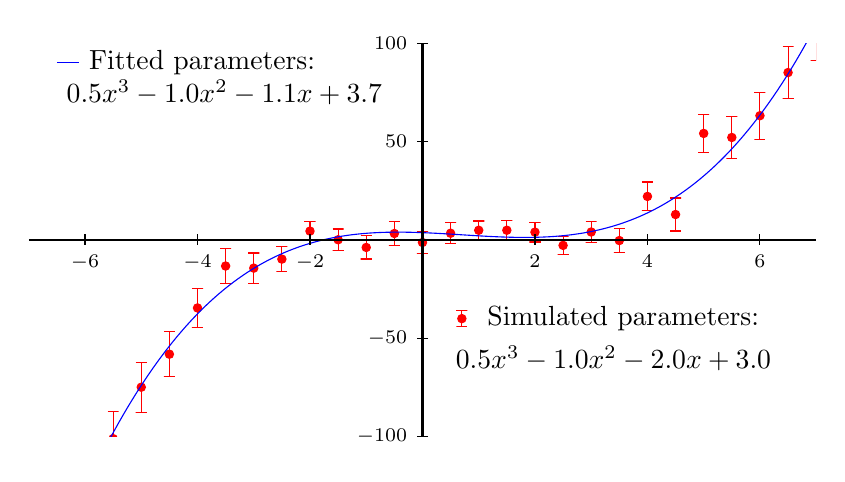
\begin{tikzpicture}
\begin{scope}[]
\pgfpathmoveto{ \pgfpointadd{\pgfpointxy {0.0} {0.0}} {\pgfpoint{0cm}{0cm}} }
\pgfpathlineto{ \pgfpointadd{\pgfpointxy {0.0} {0.0}} {\pgfpoint{10cm}{0cm}} }
\pgfpathlineto{ \pgfpointadd{\pgfpointxy {0.0} {0.0}} {\pgfpoint{10cm}{5cm}} }
\pgfpathlineto{ \pgfpointadd{\pgfpointxy {0.0} {0.0}} {\pgfpoint{0cm}{5cm}} }
\pgfpathclose
\pgfusepath{  clip, }
\begin{scope}[shift={(0.0,0.0)}]
\pgfsetxvec{\pgfpoint{0.71428573cm}{0cm}}
\pgfsetyvec{\pgfpoint{0cm}{0.025cm}}
\begin{scope}[shift={(7.0,100.0)}]
\begin{scope}[draw=red,fill=red]
\pgfpathmoveto{ \pgfpointadd{\pgfpointxy {-10.0} {-545.4404344594064}} {\pgfpoint{-2pt}{0}} }
\pgfpathlineto{ \pgfpointadd{\pgfpointxy {-10.0} {-545.4404344594064}} {\pgfpoint{2pt}{0}} }
\pgfpathlineto{ \pgfpointadd{\pgfpointxy {-10.0} {-545.4404344594064}} {\pgfpoint{0pt}{0}} }
\pgfpathlineto{ \pgfpointadd{\pgfpointxy {-10.0} {-601.4820830572636}} {\pgfpoint{0pt}{0}} }
\pgfpathlineto{ \pgfpointadd{\pgfpointxy {-10.0} {-601.4820830572636}} {\pgfpoint{-2pt}{0}} }
\pgfpathlineto{ \pgfpointadd{\pgfpointxy {-10.0} {-601.4820830572636}} {\pgfpoint{2pt}{0}} }
\pgfusepath{ stroke, }
\node at (-10.0,-573.461258758335) [draw=red,fill=red,circle,inner sep=0.0pt,minimum width =3.0pt,minimum height=3.0pt] {};
\end{scope}
\begin{scope}[draw=red,fill=red]
\pgfpathmoveto{ \pgfpointadd{\pgfpointxy {-9.5} {-447.18384020848845}} {\pgfpoint{-2pt}{0}} }
\pgfpathlineto{ \pgfpointadd{\pgfpointxy {-9.5} {-447.18384020848845}} {\pgfpoint{2pt}{0}} }
\pgfpathlineto{ \pgfpointadd{\pgfpointxy {-9.5} {-447.18384020848845}} {\pgfpoint{0pt}{0}} }
\pgfpathlineto{ \pgfpointadd{\pgfpointxy {-9.5} {-499.76803023141025}} {\pgfpoint{0pt}{0}} }
\pgfpathlineto{ \pgfpointadd{\pgfpointxy {-9.5} {-499.76803023141025}} {\pgfpoint{-2pt}{0}} }
\pgfpathlineto{ \pgfpointadd{\pgfpointxy {-9.5} {-499.76803023141025}} {\pgfpoint{2pt}{0}} }
\pgfusepath{ stroke, }
\node at (-9.5,-473.47593521994935) [draw=red,fill=red,circle,inner sep=0.0pt,minimum width =3.0pt,minimum height=3.0pt] {};
\end{scope}
\begin{scope}[draw=red,fill=red]
\pgfpathmoveto{ \pgfpointadd{\pgfpointxy {-9.0} {-393.55704978345085}} {\pgfpoint{-2pt}{0}} }
\pgfpathlineto{ \pgfpointadd{\pgfpointxy {-9.0} {-393.55704978345085}} {\pgfpoint{2pt}{0}} }
\pgfpathlineto{ \pgfpointadd{\pgfpointxy {-9.0} {-393.55704978345085}} {\pgfpoint{0pt}{0}} }
\pgfpathlineto{ \pgfpointadd{\pgfpointxy {-9.0} {-442.7638453395239}} {\pgfpoint{0pt}{0}} }
\pgfpathlineto{ \pgfpointadd{\pgfpointxy {-9.0} {-442.7638453395239}} {\pgfpoint{-2pt}{0}} }
\pgfpathlineto{ \pgfpointadd{\pgfpointxy {-9.0} {-442.7638453395239}} {\pgfpoint{2pt}{0}} }
\pgfusepath{ stroke, }
\node at (-9.0,-418.1604475614874) [draw=red,fill=red,circle,inner sep=0.0pt,minimum width =3.0pt,minimum height=3.0pt] {};
\end{scope}
\begin{scope}[draw=red,fill=red]
\pgfpathmoveto{ \pgfpointadd{\pgfpointxy {-8.5} {-308.27959989427444}} {\pgfpoint{-2pt}{0}} }
\pgfpathlineto{ \pgfpointadd{\pgfpointxy {-8.5} {-308.27959989427444}} {\pgfpoint{2pt}{0}} }
\pgfpathlineto{ \pgfpointadd{\pgfpointxy {-8.5} {-308.27959989427444}} {\pgfpoint{0pt}{0}} }
\pgfpathlineto{ \pgfpointadd{\pgfpointxy {-8.5} {-354.1906800688092}} {\pgfpoint{0pt}{0}} }
\pgfpathlineto{ \pgfpointadd{\pgfpointxy {-8.5} {-354.1906800688092}} {\pgfpoint{-2pt}{0}} }
\pgfpathlineto{ \pgfpointadd{\pgfpointxy {-8.5} {-354.1906800688092}} {\pgfpoint{2pt}{0}} }
\pgfusepath{ stroke, }
\node at (-8.5,-331.2351399815418) [draw=red,fill=red,circle,inner sep=0.0pt,minimum width =3.0pt,minimum height=3.0pt] {};
\end{scope}
\begin{scope}[draw=red,fill=red]
\pgfpathmoveto{ \pgfpointadd{\pgfpointxy {-8.0} {-239.37963398853427}} {\pgfpoint{-2pt}{0}} }
\pgfpathlineto{ \pgfpointadd{\pgfpointxy {-8.0} {-239.37963398853427}} {\pgfpoint{2pt}{0}} }
\pgfpathlineto{ \pgfpointadd{\pgfpointxy {-8.0} {-239.37963398853427}} {\pgfpoint{0pt}{0}} }
\pgfpathlineto{ \pgfpointadd{\pgfpointxy {-8.0} {-282.0783371343292}} {\pgfpoint{0pt}{0}} }
\pgfpathlineto{ \pgfpointadd{\pgfpointxy {-8.0} {-282.0783371343292}} {\pgfpoint{-2pt}{0}} }
\pgfpathlineto{ \pgfpointadd{\pgfpointxy {-8.0} {-282.0783371343292}} {\pgfpoint{2pt}{0}} }
\pgfusepath{ stroke, }
\node at (-8.0,-260.7289855614317) [draw=red,fill=red,circle,inner sep=0.0pt,minimum width =3.0pt,minimum height=3.0pt] {};
\end{scope}
\begin{scope}[draw=red,fill=red]
\pgfpathmoveto{ \pgfpointadd{\pgfpointxy {-7.5} {-197.49030193181449}} {\pgfpoint{-2pt}{0}} }
\pgfpathlineto{ \pgfpointadd{\pgfpointxy {-7.5} {-197.49030193181449}} {\pgfpoint{2pt}{0}} }
\pgfpathlineto{ \pgfpointadd{\pgfpointxy {-7.5} {-197.49030193181449}} {\pgfpoint{0pt}{0}} }
\pgfpathlineto{ \pgfpointadd{\pgfpointxy {-7.5} {-237.06164970158824}} {\pgfpoint{0pt}{0}} }
\pgfpathlineto{ \pgfpointadd{\pgfpointxy {-7.5} {-237.06164970158824}} {\pgfpoint{-2pt}{0}} }
\pgfpathlineto{ \pgfpointadd{\pgfpointxy {-7.5} {-237.06164970158824}} {\pgfpoint{2pt}{0}} }
\pgfusepath{ stroke, }
\node at (-7.5,-217.27597581670136) [draw=red,fill=red,circle,inner sep=0.0pt,minimum width =3.0pt,minimum height=3.0pt] {};
\end{scope}
\begin{scope}[draw=red,fill=red]
\pgfpathmoveto{ \pgfpointadd{\pgfpointxy {-7.0} {-205.56046021847214}} {\pgfpoint{-2pt}{0}} }
\pgfpathlineto{ \pgfpointadd{\pgfpointxy {-7.0} {-205.56046021847214}} {\pgfpoint{2pt}{0}} }
\pgfpathlineto{ \pgfpointadd{\pgfpointxy {-7.0} {-205.56046021847214}} {\pgfpoint{0pt}{0}} }
\pgfpathlineto{ \pgfpointadd{\pgfpointxy {-7.0} {-242.09114545384637}} {\pgfpoint{0pt}{0}} }
\pgfpathlineto{ \pgfpointadd{\pgfpointxy {-7.0} {-242.09114545384637}} {\pgfpoint{-2pt}{0}} }
\pgfpathlineto{ \pgfpointadd{\pgfpointxy {-7.0} {-242.09114545384637}} {\pgfpoint{2pt}{0}} }
\pgfusepath{ stroke, }
\node at (-7.0,-223.82580283615926) [draw=red,fill=red,circle,inner sep=0.0pt,minimum width =3.0pt,minimum height=3.0pt] {};
\end{scope}
\begin{scope}[draw=red,fill=red]
\pgfpathmoveto{ \pgfpointadd{\pgfpointxy {-6.5} {-139.84137726003047}} {\pgfpoint{-2pt}{0}} }
\pgfpathlineto{ \pgfpointadd{\pgfpointxy {-6.5} {-139.84137726003047}} {\pgfpoint{2pt}{0}} }
\pgfpathlineto{ \pgfpointadd{\pgfpointxy {-6.5} {-139.84137726003047}} {\pgfpoint{0pt}{0}} }
\pgfpathlineto{ \pgfpointadd{\pgfpointxy {-6.5} {-173.41968838488776}} {\pgfpoint{0pt}{0}} }
\pgfpathlineto{ \pgfpointadd{\pgfpointxy {-6.5} {-173.41968838488776}} {\pgfpoint{-2pt}{0}} }
\pgfpathlineto{ \pgfpointadd{\pgfpointxy {-6.5} {-173.41968838488776}} {\pgfpoint{2pt}{0}} }
\pgfusepath{ stroke, }
\node at (-6.5,-156.63053282245912) [draw=red,fill=red,circle,inner sep=0.0pt,minimum width =3.0pt,minimum height=3.0pt] {};
\end{scope}
\begin{scope}[draw=red,fill=red]
\pgfpathmoveto{ \pgfpointadd{\pgfpointxy {-6.0} {-137.03933110451544}} {\pgfpoint{-2pt}{0}} }
\pgfpathlineto{ \pgfpointadd{\pgfpointxy {-6.0} {-137.03933110451544}} {\pgfpoint{2pt}{0}} }
\pgfpathlineto{ \pgfpointadd{\pgfpointxy {-6.0} {-137.03933110451544}} {\pgfpoint{0pt}{0}} }
\pgfpathlineto{ \pgfpointadd{\pgfpointxy {-6.0} {-167.75496448771656}} {\pgfpoint{0pt}{0}} }
\pgfpathlineto{ \pgfpointadd{\pgfpointxy {-6.0} {-167.75496448771656}} {\pgfpoint{-2pt}{0}} }
\pgfpathlineto{ \pgfpointadd{\pgfpointxy {-6.0} {-167.75496448771656}} {\pgfpoint{2pt}{0}} }
\pgfusepath{ stroke, }
\node at (-6.0,-152.397147796116) [draw=red,fill=red,circle,inner sep=0.0pt,minimum width =3.0pt,minimum height=3.0pt] {};
\end{scope}
\begin{scope}[draw=red,fill=red]
\pgfpathmoveto{ \pgfpointadd{\pgfpointxy {-5.5} {-86.99694085231602}} {\pgfpoint{-2pt}{0}} }
\pgfpathlineto{ \pgfpointadd{\pgfpointxy {-5.5} {-86.99694085231602}} {\pgfpoint{2pt}{0}} }
\pgfpathlineto{ \pgfpointadd{\pgfpointxy {-5.5} {-86.99694085231602}} {\pgfpoint{0pt}{0}} }
\pgfpathlineto{ \pgfpointadd{\pgfpointxy {-5.5} {-114.94061152749515}} {\pgfpoint{0pt}{0}} }
\pgfpathlineto{ \pgfpointadd{\pgfpointxy {-5.5} {-114.94061152749515}} {\pgfpoint{-2pt}{0}} }
\pgfpathlineto{ \pgfpointadd{\pgfpointxy {-5.5} {-114.94061152749515}} {\pgfpoint{2pt}{0}} }
\pgfusepath{ stroke, }
\node at (-5.5,-100.96877618990558) [draw=red,fill=red,circle,inner sep=0.0pt,minimum width =3.0pt,minimum height=3.0pt] {};
\end{scope}
\begin{scope}[draw=red,fill=red]
\pgfpathmoveto{ \pgfpointadd{\pgfpointxy {-5.0} {-62.20168630127382}} {\pgfpoint{-2pt}{0}} }
\pgfpathlineto{ \pgfpointadd{\pgfpointxy {-5.0} {-62.20168630127382}} {\pgfpoint{2pt}{0}} }
\pgfpathlineto{ \pgfpointadd{\pgfpointxy {-5.0} {-62.20168630127382}} {\pgfpoint{0pt}{0}} }
\pgfpathlineto{ \pgfpointadd{\pgfpointxy {-5.0} {-87.46436280290588}} {\pgfpoint{0pt}{0}} }
\pgfpathlineto{ \pgfpointadd{\pgfpointxy {-5.0} {-87.46436280290588}} {\pgfpoint{-2pt}{0}} }
\pgfpathlineto{ \pgfpointadd{\pgfpointxy {-5.0} {-87.46436280290588}} {\pgfpoint{2pt}{0}} }
\pgfusepath{ stroke, }
\node at (-5.0,-74.83302455208985) [draw=red,fill=red,circle,inner sep=0.0pt,minimum width =3.0pt,minimum height=3.0pt] {};
\end{scope}
\begin{scope}[draw=red,fill=red]
\pgfpathmoveto{ \pgfpointadd{\pgfpointxy {-4.5} {-46.726130851753226}} {\pgfpoint{-2pt}{0}} }
\pgfpathlineto{ \pgfpointadd{\pgfpointxy {-4.5} {-46.726130851753226}} {\pgfpoint{2pt}{0}} }
\pgfpathlineto{ \pgfpointadd{\pgfpointxy {-4.5} {-46.726130851753226}} {\pgfpoint{0pt}{0}} }
\pgfpathlineto{ \pgfpointadd{\pgfpointxy {-4.5} {-69.39753160287444}} {\pgfpoint{0pt}{0}} }
\pgfpathlineto{ \pgfpointadd{\pgfpointxy {-4.5} {-69.39753160287444}} {\pgfpoint{-2pt}{0}} }
\pgfpathlineto{ \pgfpointadd{\pgfpointxy {-4.5} {-69.39753160287444}} {\pgfpoint{2pt}{0}} }
\pgfusepath{ stroke, }
\node at (-4.5,-58.06183122731383) [draw=red,fill=red,circle,inner sep=0.0pt,minimum width =3.0pt,minimum height=3.0pt] {};
\end{scope}
\begin{scope}[draw=red,fill=red]
\pgfpathmoveto{ \pgfpointadd{\pgfpointxy {-4.0} {-24.46841123687355}} {\pgfpoint{-2pt}{0}} }
\pgfpathlineto{ \pgfpointadd{\pgfpointxy {-4.0} {-24.46841123687355}} {\pgfpoint{2pt}{0}} }
\pgfpathlineto{ \pgfpointadd{\pgfpointxy {-4.0} {-24.46841123687355}} {\pgfpoint{0pt}{0}} }
\pgfpathlineto{ \pgfpointadd{\pgfpointxy {-4.0} {-44.63393629746999}} {\pgfpoint{0pt}{0}} }
\pgfpathlineto{ \pgfpointadd{\pgfpointxy {-4.0} {-44.63393629746999}} {\pgfpoint{-2pt}{0}} }
\pgfpathlineto{ \pgfpointadd{\pgfpointxy {-4.0} {-44.63393629746999}} {\pgfpoint{2pt}{0}} }
\pgfusepath{ stroke, }
\node at (-4.0,-34.55117376717177) [draw=red,fill=red,circle,inner sep=0.0pt,minimum width =3.0pt,minimum height=3.0pt] {};
\end{scope}
\begin{scope}[draw=red,fill=red]
\pgfpathmoveto{ \pgfpointadd{\pgfpointxy {-3.5} {-4.3839808804357165}} {\pgfpoint{-2pt}{0}} }
\pgfpathlineto{ \pgfpointadd{\pgfpointxy {-3.5} {-4.3839808804357165}} {\pgfpoint{2pt}{0}} }
\pgfpathlineto{ \pgfpointadd{\pgfpointxy {-3.5} {-4.3839808804357165}} {\pgfpoint{0pt}{0}} }
\pgfpathlineto{ \pgfpointadd{\pgfpointxy {-3.5} {-22.117942047401606}} {\pgfpoint{0pt}{0}} }
\pgfpathlineto{ \pgfpointadd{\pgfpointxy {-3.5} {-22.117942047401606}} {\pgfpoint{-2pt}{0}} }
\pgfpathlineto{ \pgfpointadd{\pgfpointxy {-3.5} {-22.117942047401606}} {\pgfpoint{2pt}{0}} }
\pgfusepath{ stroke, }
\node at (-3.5,-13.250961463918662) [draw=red,fill=red,circle,inner sep=0.0pt,minimum width =3.0pt,minimum height=3.0pt] {};
\end{scope}
\begin{scope}[draw=red,fill=red]
\pgfpathmoveto{ \pgfpointadd{\pgfpointxy {-3.0} {-6.647445276239654}} {\pgfpoint{-2pt}{0}} }
\pgfpathlineto{ \pgfpointadd{\pgfpointxy {-3.0} {-6.647445276239654}} {\pgfpoint{2pt}{0}} }
\pgfpathlineto{ \pgfpointadd{\pgfpointxy {-3.0} {-6.647445276239654}} {\pgfpoint{0pt}{0}} }
\pgfpathlineto{ \pgfpointadd{\pgfpointxy {-3.0} {-21.995914504589187}} {\pgfpoint{0pt}{0}} }
\pgfpathlineto{ \pgfpointadd{\pgfpointxy {-3.0} {-21.995914504589187}} {\pgfpoint{-2pt}{0}} }
\pgfpathlineto{ \pgfpointadd{\pgfpointxy {-3.0} {-21.995914504589187}} {\pgfpoint{2pt}{0}} }
\pgfusepath{ stroke, }
\node at (-3.0,-14.321679890414421) [draw=red,fill=red,circle,inner sep=0.0pt,minimum width =3.0pt,minimum height=3.0pt] {};
\end{scope}
\begin{scope}[draw=red,fill=red]
\pgfpathmoveto{ \pgfpointadd{\pgfpointxy {-2.5} {-3.2769548489061266}} {\pgfpoint{-2pt}{0}} }
\pgfpathlineto{ \pgfpointadd{\pgfpointxy {-2.5} {-3.2769548489061266}} {\pgfpoint{2pt}{0}} }
\pgfpathlineto{ \pgfpointadd{\pgfpointxy {-2.5} {-3.2769548489061266}} {\pgfpoint{0pt}{0}} }
\pgfpathlineto{ \pgfpointadd{\pgfpointxy {-2.5} {-16.20138374980418}} {\pgfpoint{0pt}{0}} }
\pgfpathlineto{ \pgfpointadd{\pgfpointxy {-2.5} {-16.20138374980418}} {\pgfpoint{-2pt}{0}} }
\pgfpathlineto{ \pgfpointadd{\pgfpointxy {-2.5} {-16.20138374980418}} {\pgfpoint{2pt}{0}} }
\pgfusepath{ stroke, }
\node at (-2.5,-9.739169299355153) [draw=red,fill=red,circle,inner sep=0.0pt,minimum width =3.0pt,minimum height=3.0pt] {};
\end{scope}
\begin{scope}[draw=red,fill=red]
\pgfpathmoveto{ \pgfpointadd{\pgfpointxy {-2.0} {9.4928432370132}} {\pgfpoint{-2pt}{0}} }
\pgfpathlineto{ \pgfpointadd{\pgfpointxy {-2.0} {9.4928432370132}} {\pgfpoint{2pt}{0}} }
\pgfpathlineto{ \pgfpointadd{\pgfpointxy {-2.0} {9.4928432370132}} {\pgfpoint{0pt}{0}} }
\pgfpathlineto{ \pgfpointadd{\pgfpointxy {-2.0} {-0.5071567629867992}} {\pgfpoint{0pt}{0}} }
\pgfpathlineto{ \pgfpointadd{\pgfpointxy {-2.0} {-0.5071567629867992}} {\pgfpoint{-2pt}{0}} }
\pgfpathlineto{ \pgfpointadd{\pgfpointxy {-2.0} {-0.5071567629867992}} {\pgfpoint{2pt}{0}} }
\pgfusepath{ stroke, }
\node at (-2.0,4.492843237013201) [draw=red,fill=red,circle,inner sep=0.0pt,minimum width =3.0pt,minimum height=3.0pt] {};
\end{scope}
\begin{scope}[draw=red,fill=red]
\pgfpathmoveto{ \pgfpointadd{\pgfpointxy {-1.5} {5.5385561325248664}} {\pgfpoint{-2pt}{0}} }
\pgfpathlineto{ \pgfpointadd{\pgfpointxy {-1.5} {5.5385561325248664}} {\pgfpoint{2pt}{0}} }
\pgfpathlineto{ \pgfpointadd{\pgfpointxy {-1.5} {5.5385561325248664}} {\pgfpoint{0pt}{0}} }
\pgfpathlineto{ \pgfpointadd{\pgfpointxy {-1.5} {-5.333725190744148}} {\pgfpoint{0pt}{0}} }
\pgfpathlineto{ \pgfpointadd{\pgfpointxy {-1.5} {-5.333725190744148}} {\pgfpoint{-2pt}{0}} }
\pgfpathlineto{ \pgfpointadd{\pgfpointxy {-1.5} {-5.333725190744148}} {\pgfpoint{2pt}{0}} }
\pgfusepath{ stroke, }
\node at (-1.5,0.10241547089035907) [draw=red,fill=red,circle,inner sep=0.0pt,minimum width =3.0pt,minimum height=3.0pt] {};
\end{scope}
\begin{scope}[draw=red,fill=red]
\pgfpathmoveto{ \pgfpointadd{\pgfpointxy {-1.0} {2.0474943682430817}} {\pgfpoint{-2pt}{0}} }
\pgfpathlineto{ \pgfpointadd{\pgfpointxy {-1.0} {2.0474943682430817}} {\pgfpoint{2pt}{0}} }
\pgfpathlineto{ \pgfpointadd{\pgfpointxy {-1.0} {2.0474943682430817}} {\pgfpoint{0pt}{0}} }
\pgfpathlineto{ \pgfpointadd{\pgfpointxy {-1.0} {-9.694163018530858}} {\pgfpoint{0pt}{0}} }
\pgfpathlineto{ \pgfpointadd{\pgfpointxy {-1.0} {-9.694163018530858}} {\pgfpoint{-2pt}{0}} }
\pgfpathlineto{ \pgfpointadd{\pgfpointxy {-1.0} {-9.694163018530858}} {\pgfpoint{2pt}{0}} }
\pgfusepath{ stroke, }
\node at (-1.0,-3.8233343251438887) [draw=red,fill=red,circle,inner sep=0.0pt,minimum width =3.0pt,minimum height=3.0pt] {};
\end{scope}
\begin{scope}[draw=red,fill=red]
\pgfpathmoveto{ \pgfpointadd{\pgfpointxy {-0.5} {9.199319361891407}} {\pgfpoint{-2pt}{0}} }
\pgfpathlineto{ \pgfpointadd{\pgfpointxy {-0.5} {9.199319361891407}} {\pgfpoint{2pt}{0}} }
\pgfpathlineto{ \pgfpointadd{\pgfpointxy {-0.5} {9.199319361891407}} {\pgfpoint{0pt}{0}} }
\pgfpathlineto{ \pgfpointadd{\pgfpointxy {-0.5} {-2.6412535120428977}} {\pgfpoint{0pt}{0}} }
\pgfpathlineto{ \pgfpointadd{\pgfpointxy {-0.5} {-2.6412535120428977}} {\pgfpoint{-2pt}{0}} }
\pgfpathlineto{ \pgfpointadd{\pgfpointxy {-0.5} {-2.6412535120428977}} {\pgfpoint{2pt}{0}} }
\pgfusepath{ stroke, }
\node at (-0.5,3.2790329249242545) [draw=red,fill=red,circle,inner sep=0.0pt,minimum width =3.0pt,minimum height=3.0pt] {};
\end{scope}
\begin{scope}[draw=red,fill=red]
\pgfpathmoveto{ \pgfpointadd{\pgfpointxy {0.0} {4.442405535239562}} {\pgfpoint{-2pt}{0}} }
\pgfpathlineto{ \pgfpointadd{\pgfpointxy {0.0} {4.442405535239562}} {\pgfpoint{2pt}{0}} }
\pgfpathlineto{ \pgfpointadd{\pgfpointxy {0.0} {4.442405535239562}} {\pgfpoint{0pt}{0}} }
\pgfpathlineto{ \pgfpointadd{\pgfpointxy {0.0} {-7.021696079898192}} {\pgfpoint{0pt}{0}} }
\pgfpathlineto{ \pgfpointadd{\pgfpointxy {0.0} {-7.021696079898192}} {\pgfpoint{-2pt}{0}} }
\pgfpathlineto{ \pgfpointadd{\pgfpointxy {0.0} {-7.021696079898192}} {\pgfpoint{2pt}{0}} }
\pgfusepath{ stroke, }
\node at (0.0,-1.2896452723293148) [draw=red,fill=red,circle,inner sep=0.0pt,minimum width =3.0pt,minimum height=3.0pt] {};
\end{scope}
\begin{scope}[draw=red,fill=red]
\pgfpathmoveto{ \pgfpointadd{\pgfpointxy {0.5} {8.757501632045631}} {\pgfpoint{-2pt}{0}} }
\pgfpathlineto{ \pgfpointadd{\pgfpointxy {0.5} {8.757501632045631}} {\pgfpoint{2pt}{0}} }
\pgfpathlineto{ \pgfpointadd{\pgfpointxy {0.5} {8.757501632045631}} {\pgfpoint{0pt}{0}} }
\pgfpathlineto{ \pgfpointadd{\pgfpointxy {0.5} {-1.93508077152162}} {\pgfpoint{0pt}{0}} }
\pgfpathlineto{ \pgfpointadd{\pgfpointxy {0.5} {-1.93508077152162}} {\pgfpoint{-2pt}{0}} }
\pgfpathlineto{ \pgfpointadd{\pgfpointxy {0.5} {-1.93508077152162}} {\pgfpoint{2pt}{0}} }
\pgfusepath{ stroke, }
\node at (0.5,3.411210430262006) [draw=red,fill=red,circle,inner sep=0.0pt,minimum width =3.0pt,minimum height=3.0pt] {};
\end{scope}
\begin{scope}[draw=red,fill=red]
\pgfpathmoveto{ \pgfpointadd{\pgfpointxy {1.0} {9.619207276103703}} {\pgfpoint{-2pt}{0}} }
\pgfpathlineto{ \pgfpointadd{\pgfpointxy {1.0} {9.619207276103703}} {\pgfpoint{2pt}{0}} }
\pgfpathlineto{ \pgfpointadd{\pgfpointxy {1.0} {9.619207276103703}} {\pgfpoint{0pt}{0}} }
\pgfpathlineto{ \pgfpointadd{\pgfpointxy {1.0} {0.20499371373060704}} {\pgfpoint{0pt}{0}} }
\pgfpathlineto{ \pgfpointadd{\pgfpointxy {1.0} {0.20499371373060704}} {\pgfpoint{-2pt}{0}} }
\pgfpathlineto{ \pgfpointadd{\pgfpointxy {1.0} {0.20499371373060704}} {\pgfpoint{2pt}{0}} }
\pgfusepath{ stroke, }
\node at (1.0,4.912100494917155) [draw=red,fill=red,circle,inner sep=0.0pt,minimum width =3.0pt,minimum height=3.0pt] {};
\end{scope}
\begin{scope}[draw=red,fill=red]
\pgfpathmoveto{ \pgfpointadd{\pgfpointxy {1.5} {9.676990570717388}} {\pgfpoint{-2pt}{0}} }
\pgfpathlineto{ \pgfpointadd{\pgfpointxy {1.5} {9.676990570717388}} {\pgfpoint{2pt}{0}} }
\pgfpathlineto{ \pgfpointadd{\pgfpointxy {1.5} {9.676990570717388}} {\pgfpoint{0pt}{0}} }
\pgfpathlineto{ \pgfpointadd{\pgfpointxy {1.5} {0.176990570717388}} {\pgfpoint{0pt}{0}} }
\pgfpathlineto{ \pgfpointadd{\pgfpointxy {1.5} {0.176990570717388}} {\pgfpoint{-2pt}{0}} }
\pgfpathlineto{ \pgfpointadd{\pgfpointxy {1.5} {0.176990570717388}} {\pgfpoint{2pt}{0}} }
\pgfusepath{ stroke, }
\node at (1.5,4.926990570717388) [draw=red,fill=red,circle,inner sep=0.0pt,minimum width =3.0pt,minimum height=3.0pt] {};
\end{scope}
\begin{scope}[draw=red,fill=red]
\pgfpathmoveto{ \pgfpointadd{\pgfpointxy {2.0} {8.978212194906977}} {\pgfpoint{-2pt}{0}} }
\pgfpathlineto{ \pgfpointadd{\pgfpointxy {2.0} {8.978212194906977}} {\pgfpoint{2pt}{0}} }
\pgfpathlineto{ \pgfpointadd{\pgfpointxy {2.0} {8.978212194906977}} {\pgfpoint{0pt}{0}} }
\pgfpathlineto{ \pgfpointadd{\pgfpointxy {2.0} {-1.0217878050930222}} {\pgfpoint{0pt}{0}} }
\pgfpathlineto{ \pgfpointadd{\pgfpointxy {2.0} {-1.0217878050930222}} {\pgfpoint{-2pt}{0}} }
\pgfpathlineto{ \pgfpointadd{\pgfpointxy {2.0} {-1.0217878050930222}} {\pgfpoint{2pt}{0}} }
\pgfusepath{ stroke, }
\node at (2.0,3.9782121949069778) [draw=red,fill=red,circle,inner sep=0.0pt,minimum width =3.0pt,minimum height=3.0pt] {};
\end{scope}
\begin{scope}[draw=red,fill=red]
\pgfpathmoveto{ \pgfpointadd{\pgfpointxy {2.5} {1.8969141840287458}} {\pgfpoint{-2pt}{0}} }
\pgfpathlineto{ \pgfpointadd{\pgfpointxy {2.5} {1.8969141840287458}} {\pgfpoint{2pt}{0}} }
\pgfpathlineto{ \pgfpointadd{\pgfpointxy {2.5} {1.8969141840287458}} {\pgfpoint{0pt}{0}} }
\pgfpathlineto{ \pgfpointadd{\pgfpointxy {2.5} {-7.425961471503549}} {\pgfpoint{0pt}{0}} }
\pgfpathlineto{ \pgfpointadd{\pgfpointxy {2.5} {-7.425961471503549}} {\pgfpoint{-2pt}{0}} }
\pgfpathlineto{ \pgfpointadd{\pgfpointxy {2.5} {-7.425961471503549}} {\pgfpoint{2pt}{0}} }
\pgfusepath{ stroke, }
\node at (2.5,-2.7645236437374017) [draw=red,fill=red,circle,inner sep=0.0pt,minimum width =3.0pt,minimum height=3.0pt] {};
\end{scope}
\begin{scope}[draw=red,fill=red]
\pgfpathmoveto{ \pgfpointadd{\pgfpointxy {3.0} {9.255509543307898}} {\pgfpoint{-2pt}{0}} }
\pgfpathlineto{ \pgfpointadd{\pgfpointxy {3.0} {9.255509543307898}} {\pgfpoint{2pt}{0}} }
\pgfpathlineto{ \pgfpointadd{\pgfpointxy {3.0} {9.255509543307898}} {\pgfpoint{0pt}{0}} }
\pgfpathlineto{ \pgfpointadd{\pgfpointxy {3.0} {-1.1939801994752797}} {\pgfpoint{0pt}{0}} }
\pgfpathlineto{ \pgfpointadd{\pgfpointxy {3.0} {-1.1939801994752797}} {\pgfpoint{-2pt}{0}} }
\pgfpathlineto{ \pgfpointadd{\pgfpointxy {3.0} {-1.1939801994752797}} {\pgfpoint{2pt}{0}} }
\pgfusepath{ stroke, }
\node at (3.0,4.03076467191631) [draw=red,fill=red,circle,inner sep=0.0pt,minimum width =3.0pt,minimum height=3.0pt] {};
\end{scope}
\begin{scope}[draw=red,fill=red]
\pgfpathmoveto{ \pgfpointadd{\pgfpointxy {3.5} {5.964258662648645}} {\pgfpoint{-2pt}{0}} }
\pgfpathlineto{ \pgfpointadd{\pgfpointxy {3.5} {5.964258662648645}} {\pgfpoint{2pt}{0}} }
\pgfpathlineto{ \pgfpointadd{\pgfpointxy {3.5} {5.964258662648645}} {\pgfpoint{0pt}{0}} }
\pgfpathlineto{ \pgfpointadd{\pgfpointxy {3.5} {-6.590958126923504}} {\pgfpoint{0pt}{0}} }
\pgfpathlineto{ \pgfpointadd{\pgfpointxy {3.5} {-6.590958126923504}} {\pgfpoint{-2pt}{0}} }
\pgfpathlineto{ \pgfpointadd{\pgfpointxy {3.5} {-6.590958126923504}} {\pgfpoint{2pt}{0}} }
\pgfusepath{ stroke, }
\node at (3.5,-0.31334973213742945) [draw=red,fill=red,circle,inner sep=0.0pt,minimum width =3.0pt,minimum height=3.0pt] {};
\end{scope}
\begin{scope}[draw=red,fill=red]
\pgfpathmoveto{ \pgfpointadd{\pgfpointxy {4.0} {29.421398911157304}} {\pgfpoint{-2pt}{0}} }
\pgfpathlineto{ \pgfpointadd{\pgfpointxy {4.0} {29.421398911157304}} {\pgfpoint{2pt}{0}} }
\pgfpathlineto{ \pgfpointadd{\pgfpointxy {4.0} {29.421398911157304}} {\pgfpoint{0pt}{0}} }
\pgfpathlineto{ \pgfpointadd{\pgfpointxy {4.0} {14.788149330446506}} {\pgfpoint{0pt}{0}} }
\pgfpathlineto{ \pgfpointadd{\pgfpointxy {4.0} {14.788149330446506}} {\pgfpoint{-2pt}{0}} }
\pgfpathlineto{ \pgfpointadd{\pgfpointxy {4.0} {14.788149330446506}} {\pgfpoint{2pt}{0}} }
\pgfusepath{ stroke, }
\node at (4.0,22.104774120801906) [draw=red,fill=red,circle,inner sep=0.0pt,minimum width =3.0pt,minimum height=3.0pt] {};
\end{scope}
\begin{scope}[draw=red,fill=red]
\pgfpathmoveto{ \pgfpointadd{\pgfpointxy {4.5} {21.306695411062467}} {\pgfpoint{-2pt}{0}} }
\pgfpathlineto{ \pgfpointadd{\pgfpointxy {4.5} {21.306695411062467}} {\pgfpoint{2pt}{0}} }
\pgfpathlineto{ \pgfpointadd{\pgfpointxy {4.5} {21.306695411062467}} {\pgfpoint{0pt}{0}} }
\pgfpathlineto{ \pgfpointadd{\pgfpointxy {4.5} {4.517497495438992}} {\pgfpoint{0pt}{0}} }
\pgfpathlineto{ \pgfpointadd{\pgfpointxy {4.5} {4.517497495438992}} {\pgfpoint{-2pt}{0}} }
\pgfpathlineto{ \pgfpointadd{\pgfpointxy {4.5} {4.517497495438992}} {\pgfpoint{2pt}{0}} }
\pgfusepath{ stroke, }
\node at (4.5,12.91209645325073) [draw=red,fill=red,circle,inner sep=0.0pt,minimum width =3.0pt,minimum height=3.0pt] {};
\end{scope}
\begin{scope}[draw=red,fill=red]
\pgfpathmoveto{ \pgfpointadd{\pgfpointxy {5.0} {63.64740104424042}} {\pgfpoint{-2pt}{0}} }
\pgfpathlineto{ \pgfpointadd{\pgfpointxy {5.0} {63.64740104424042}} {\pgfpoint{2pt}{0}} }
\pgfpathlineto{ \pgfpointadd{\pgfpointxy {5.0} {63.64740104424042}} {\pgfpoint{0pt}{0}} }
\pgfpathlineto{ \pgfpointadd{\pgfpointxy {5.0} {44.60204002705316}} {\pgfpoint{0pt}{0}} }
\pgfpathlineto{ \pgfpointadd{\pgfpointxy {5.0} {44.60204002705316}} {\pgfpoint{-2pt}{0}} }
\pgfpathlineto{ \pgfpointadd{\pgfpointxy {5.0} {44.60204002705316}} {\pgfpoint{2pt}{0}} }
\pgfusepath{ stroke, }
\node at (5.0,54.12472053564679) [draw=red,fill=red,circle,inner sep=0.0pt,minimum width =3.0pt,minimum height=3.0pt] {};
\end{scope}
\begin{scope}[draw=red,fill=red]
\pgfpathmoveto{ \pgfpointadd{\pgfpointxy {5.5} {62.77248248245576}} {\pgfpoint{-2pt}{0}} }
\pgfpathlineto{ \pgfpointadd{\pgfpointxy {5.5} {62.77248248245576}} {\pgfpoint{2pt}{0}} }
\pgfpathlineto{ \pgfpointadd{\pgfpointxy {5.5} {62.77248248245576}} {\pgfpoint{0pt}{0}} }
\pgfpathlineto{ \pgfpointadd{\pgfpointxy {5.5} {41.365394804663836}} {\pgfpoint{0pt}{0}} }
\pgfpathlineto{ \pgfpointadd{\pgfpointxy {5.5} {41.365394804663836}} {\pgfpoint{-2pt}{0}} }
\pgfpathlineto{ \pgfpointadd{\pgfpointxy {5.5} {41.365394804663836}} {\pgfpoint{2pt}{0}} }
\pgfusepath{ stroke, }
\node at (5.5,52.0689386435598) [draw=red,fill=red,circle,inner sep=0.0pt,minimum width =3.0pt,minimum height=3.0pt] {};
\end{scope}
\begin{scope}[draw=red,fill=red]
\pgfpathmoveto{ \pgfpointadd{\pgfpointxy {6.0} {75.06961524037354}} {\pgfpoint{-2pt}{0}} }
\pgfpathlineto{ \pgfpointadd{\pgfpointxy {6.0} {75.06961524037354}} {\pgfpoint{2pt}{0}} }
\pgfpathlineto{ \pgfpointadd{\pgfpointxy {6.0} {75.06961524037354}} {\pgfpoint{0pt}{0}} }
\pgfpathlineto{ \pgfpointadd{\pgfpointxy {6.0} {51.195107373985984}} {\pgfpoint{0pt}{0}} }
\pgfpathlineto{ \pgfpointadd{\pgfpointxy {6.0} {51.195107373985984}} {\pgfpoint{-2pt}{0}} }
\pgfpathlineto{ \pgfpointadd{\pgfpointxy {6.0} {51.195107373985984}} {\pgfpoint{2pt}{0}} }
\pgfusepath{ stroke, }
\node at (6.0,63.13236130717976) [draw=red,fill=red,circle,inner sep=0.0pt,minimum width =3.0pt,minimum height=3.0pt] {};
\end{scope}
\begin{scope}[draw=red,fill=red]
\pgfpathmoveto{ \pgfpointadd{\pgfpointxy {6.5} {98.27282162103023}} {\pgfpoint{-2pt}{0}} }
\pgfpathlineto{ \pgfpointadd{\pgfpointxy {6.5} {98.27282162103023}} {\pgfpoint{2pt}{0}} }
\pgfpathlineto{ \pgfpointadd{\pgfpointxy {6.5} {98.27282162103023}} {\pgfpoint{0pt}{0}} }
\pgfpathlineto{ \pgfpointadd{\pgfpointxy {6.5} {71.82695487533351}} {\pgfpoint{0pt}{0}} }
\pgfpathlineto{ \pgfpointadd{\pgfpointxy {6.5} {71.82695487533351}} {\pgfpoint{-2pt}{0}} }
\pgfpathlineto{ \pgfpointadd{\pgfpointxy {6.5} {71.82695487533351}} {\pgfpoint{2pt}{0}} }
\pgfusepath{ stroke, }
\node at (6.5,85.04988824818187) [draw=red,fill=red,circle,inner sep=0.0pt,minimum width =3.0pt,minimum height=3.0pt] {};
\end{scope}
\begin{scope}[draw=red,fill=red]
\pgfpathmoveto{ \pgfpointadd{\pgfpointxy {7.0} {120.17309324555772}} {\pgfpoint{-2pt}{0}} }
\pgfpathlineto{ \pgfpointadd{\pgfpointxy {7.0} {120.17309324555772}} {\pgfpoint{2pt}{0}} }
\pgfpathlineto{ \pgfpointadd{\pgfpointxy {7.0} {120.17309324555772}} {\pgfpoint{0pt}{0}} }
\pgfpathlineto{ \pgfpointadd{\pgfpointxy {7.0} {91.05438116361485}} {\pgfpoint{0pt}{0}} }
\pgfpathlineto{ \pgfpointadd{\pgfpointxy {7.0} {91.05438116361485}} {\pgfpoint{-2pt}{0}} }
\pgfpathlineto{ \pgfpointadd{\pgfpointxy {7.0} {91.05438116361485}} {\pgfpoint{2pt}{0}} }
\pgfusepath{ stroke, }
\node at (7.0,105.61373720458629) [draw=red,fill=red,circle,inner sep=0.0pt,minimum width =3.0pt,minimum height=3.0pt] {};
\end{scope}
\begin{scope}[draw=red,fill=red]
\pgfpathmoveto{ \pgfpointadd{\pgfpointxy {7.5} {151.1696495331387}} {\pgfpoint{-2pt}{0}} }
\pgfpathlineto{ \pgfpointadd{\pgfpointxy {7.5} {151.1696495331387}} {\pgfpoint{2pt}{0}} }
\pgfpathlineto{ \pgfpointadd{\pgfpointxy {7.5} {151.1696495331387}} {\pgfpoint{0pt}{0}} }
\pgfpathlineto{ \pgfpointadd{\pgfpointxy {7.5} {119.27927490233813}} {\pgfpoint{0pt}{0}} }
\pgfpathlineto{ \pgfpointadd{\pgfpointxy {7.5} {119.27927490233813}} {\pgfpoint{-2pt}{0}} }
\pgfpathlineto{ \pgfpointadd{\pgfpointxy {7.5} {119.27927490233813}} {\pgfpoint{2pt}{0}} }
\pgfusepath{ stroke, }
\node at (7.5,135.22446221773842) [draw=red,fill=red,circle,inner sep=0.0pt,minimum width =3.0pt,minimum height=3.0pt] {};
\end{scope}
\begin{scope}[draw=red,fill=red]
\pgfpathmoveto{ \pgfpointadd{\pgfpointxy {8.0} {174.93586539469865}} {\pgfpoint{-2pt}{0}} }
\pgfpathlineto{ \pgfpointadd{\pgfpointxy {8.0} {174.93586539469865}} {\pgfpoint{2pt}{0}} }
\pgfpathlineto{ \pgfpointadd{\pgfpointxy {8.0} {174.93586539469865}} {\pgfpoint{0pt}{0}} }
\pgfpathlineto{ \pgfpointadd{\pgfpointxy {8.0} {140.17768907417937}} {\pgfpoint{0pt}{0}} }
\pgfpathlineto{ \pgfpointadd{\pgfpointxy {8.0} {140.17768907417937}} {\pgfpoint{-2pt}{0}} }
\pgfpathlineto{ \pgfpointadd{\pgfpointxy {8.0} {140.17768907417937}} {\pgfpoint{2pt}{0}} }
\pgfusepath{ stroke, }
\node at (8.0,157.556777234439) [draw=red,fill=red,circle,inner sep=0.0pt,minimum width =3.0pt,minimum height=3.0pt] {};
\end{scope}
\begin{scope}[draw=red,fill=red]
\pgfpathmoveto{ \pgfpointadd{\pgfpointxy {8.5} {210.68882219254994}} {\pgfpoint{-2pt}{0}} }
\pgfpathlineto{ \pgfpointadd{\pgfpointxy {8.5} {210.68882219254994}} {\pgfpoint{2pt}{0}} }
\pgfpathlineto{ \pgfpointadd{\pgfpointxy {8.5} {210.68882219254994}} {\pgfpoint{0pt}{0}} }
\pgfpathlineto{ \pgfpointadd{\pgfpointxy {8.5} {172.96929998912276}} {\pgfpoint{0pt}{0}} }
\pgfpathlineto{ \pgfpointadd{\pgfpointxy {8.5} {172.96929998912276}} {\pgfpoint{-2pt}{0}} }
\pgfpathlineto{ \pgfpointadd{\pgfpointxy {8.5} {172.96929998912276}} {\pgfpoint{2pt}{0}} }
\pgfusepath{ stroke, }
\node at (8.5,191.82906109083635) [draw=red,fill=red,circle,inner sep=0.0pt,minimum width =3.0pt,minimum height=3.0pt] {};
\end{scope}
\begin{scope}[draw=red,fill=red]
\pgfpathmoveto{ \pgfpointadd{\pgfpointxy {9.0} {290.0647928672955}} {\pgfpoint{-2pt}{0}} }
\pgfpathlineto{ \pgfpointadd{\pgfpointxy {9.0} {290.0647928672955}} {\pgfpoint{2pt}{0}} }
\pgfpathlineto{ \pgfpointadd{\pgfpointxy {9.0} {290.0647928672955}} {\pgfpoint{0pt}{0}} }
\pgfpathlineto{ \pgfpointadd{\pgfpointxy {9.0} {249.29285365094765}} {\pgfpoint{0pt}{0}} }
\pgfpathlineto{ \pgfpointadd{\pgfpointxy {9.0} {249.29285365094765}} {\pgfpoint{-2pt}{0}} }
\pgfpathlineto{ \pgfpointadd{\pgfpointxy {9.0} {249.29285365094765}} {\pgfpoint{2pt}{0}} }
\pgfusepath{ stroke, }
\node at (9.0,269.6788232591216) [draw=red,fill=red,circle,inner sep=0.0pt,minimum width =3.0pt,minimum height=3.0pt] {};
\end{scope}
\begin{scope}[draw=red,fill=red]
\pgfpathmoveto{ \pgfpointadd{\pgfpointxy {9.5} {314.0828958330366}} {\pgfpoint{-2pt}{0}} }
\pgfpathlineto{ \pgfpointadd{\pgfpointxy {9.5} {314.0828958330366}} {\pgfpoint{2pt}{0}} }
\pgfpathlineto{ \pgfpointadd{\pgfpointxy {9.5} {314.0828958330366}} {\pgfpoint{0pt}{0}} }
\pgfpathlineto{ \pgfpointadd{\pgfpointxy {9.5} {270.1698062973256}} {\pgfpoint{0pt}{0}} }
\pgfpathlineto{ \pgfpointadd{\pgfpointxy {9.5} {270.1698062973256}} {\pgfpoint{-2pt}{0}} }
\pgfpathlineto{ \pgfpointadd{\pgfpointxy {9.5} {270.1698062973256}} {\pgfpoint{2pt}{0}} }
\pgfusepath{ stroke, }
\node at (9.5,292.1263510651811) [draw=red,fill=red,circle,inner sep=0.0pt,minimum width =3.0pt,minimum height=3.0pt] {};
\end{scope}
\begin{scope}[draw=red,fill=red]
\pgfpathmoveto{ \pgfpointadd{\pgfpointxy {10.0} {418.424634994198}} {\pgfpoint{-2pt}{0}} }
\pgfpathlineto{ \pgfpointadd{\pgfpointxy {10.0} {418.424634994198}} {\pgfpoint{2pt}{0}} }
\pgfpathlineto{ \pgfpointadd{\pgfpointxy {10.0} {418.424634994198}} {\pgfpoint{0pt}{0}} }
\pgfpathlineto{ \pgfpointadd{\pgfpointxy {10.0} {371.2838634126362}} {\pgfpoint{0pt}{0}} }
\pgfpathlineto{ \pgfpointadd{\pgfpointxy {10.0} {371.2838634126362}} {\pgfpoint{-2pt}{0}} }
\pgfpathlineto{ \pgfpointadd{\pgfpointxy {10.0} {371.2838634126362}} {\pgfpoint{2pt}{0}} }
\pgfusepath{ stroke, }
\node at (10.0,394.8542492034171) [draw=red,fill=red,circle,inner sep=0.0pt,minimum width =3.0pt,minimum height=3.0pt] {};
\end{scope}
\end{scope}
\pgfsetxvec{\pgfpoint{1cm}{0cm}}
\pgfsetyvec{\pgfpoint{0cm}{1cm}}
\end{scope}
\end{scope}
\begin{scope}[draw=red,fill=red]
\pgfpathmoveto{ \pgfpointadd{\pgfpointxy {5.5} {1.6}} {\pgfpoint{-2pt}{0}} }
\pgfpathlineto{ \pgfpointadd{\pgfpointxy {5.5} {1.6}} {\pgfpoint{2pt}{0}} }
\pgfpathlineto{ \pgfpointadd{\pgfpointxy {5.5} {1.6}} {\pgfpoint{0pt}{0}} }
\pgfpathlineto{ \pgfpointadd{\pgfpointxy {5.5} {1.4}} {\pgfpoint{0pt}{0}} }
\pgfpathlineto{ \pgfpointadd{\pgfpointxy {5.5} {1.4}} {\pgfpoint{-2pt}{0}} }
\pgfpathlineto{ \pgfpointadd{\pgfpointxy {5.5} {1.4}} {\pgfpoint{2pt}{0}} }
\pgfusepath{ stroke, }
\node at (5.5,1.5) [draw=red,fill=red,circle,inner sep=0.0pt,minimum width =3.0pt,minimum height=3.0pt] {};
\end{scope}
\node at (5.7000003,1.5) [right,] {Simulated parameters:};
\node at (5.3,1.0) [right,] {$0.5x^3 -1.0x^2 -2.0x +3.0$};
\begin{scope}[shift={(0.0,0.0)}]
\pgfsetxvec{\pgfpoint{0.71428573cm}{0cm}}
\pgfsetyvec{\pgfpoint{0cm}{0.025cm}}
\begin{scope}[shift={(7.0,100.0)}]
\begin{scope}[]
\pgfpathmoveto{ \pgfpointadd{\pgfpointxy {-7.0} {-100.0}} {\pgfpoint{0cm}{0cm}} }
\pgfpathlineto{ \pgfpointadd{\pgfpointxy {-7.0} {-100.0}} {\pgfpoint{10cm}{0cm}} }
\pgfpathlineto{ \pgfpointadd{\pgfpointxy {-7.0} {-100.0}} {\pgfpoint{10cm}{5cm}} }
\pgfpathlineto{ \pgfpointadd{\pgfpointxy {-7.0} {-100.0}} {\pgfpoint{0cm}{5cm}} }
\pgfpathclose
\pgfusepath{  clip, }
\begin{scope}[blue]
\pgfpathmoveto{ \pgfpointxy {-7.0} {-197.66695401534344}}
\pgfpathlineto{ \pgfpointxy {-6.93} {-192.00156064351145}}
\pgfpathlineto{ \pgfpointxy {-6.86} {-186.44155537130268}}
\pgfpathlineto{ \pgfpointxy {-6.79} {-180.9859703388876}}
\pgfpathlineto{ \pgfpointxy {-6.72} {-175.63383768643678}}
\pgfpathlineto{ \pgfpointxy {-6.65} {-170.3841895541207}}
\pgfpathlineto{ \pgfpointxy {-6.58} {-165.2360580821099}}
\pgfpathlineto{ \pgfpointxy {-6.51} {-160.18847541057488}}
\pgfpathlineto{ \pgfpointxy {-6.44} {-155.24047367968618}}
\pgfpathlineto{ \pgfpointxy {-6.37} {-150.39108502961432}}
\pgfpathlineto{ \pgfpointxy {-6.3} {-145.6393416005298}}
\pgfpathlineto{ \pgfpointxy {-6.23} {-140.98427553260316}}
\pgfpathlineto{ \pgfpointxy {-6.16} {-136.4249189660049}}
\pgfpathlineto{ \pgfpointxy {-6.09} {-131.96030404090558}}
\pgfpathlineto{ \pgfpointxy {-6.02} {-127.58946289747564}}
\pgfpathlineto{ \pgfpointxy {-5.95} {-123.31142767588568}}
\pgfpathlineto{ \pgfpointxy {-5.88} {-119.12523051630617}}
\pgfpathlineto{ \pgfpointxy {-5.81} {-115.02990355890768}}
\pgfpathlineto{ \pgfpointxy {-5.74} {-111.02447894386066}}
\pgfpathlineto{ \pgfpointxy {-5.67} {-107.1079888113357}}
\pgfpathlineto{ \pgfpointxy {-5.6} {-103.27946530150327}}
\pgfpathlineto{ \pgfpointxy {-5.53} {-99.5379405545339}}
\pgfpathlineto{ \pgfpointxy {-5.46} {-95.88244671059812}}
\pgfpathlineto{ \pgfpointxy {-5.39} {-92.31201590986646}}
\pgfpathlineto{ \pgfpointxy {-5.32} {-88.82568029250938}}
\pgfpathlineto{ \pgfpointxy {-5.25} {-85.42247199869746}}
\pgfpathlineto{ \pgfpointxy {-5.18} {-82.10142316860123}}
\pgfpathlineto{ \pgfpointxy {-5.11} {-78.86156594239115}}
\pgfpathlineto{ \pgfpointxy {-5.04} {-75.70193246023778}}
\pgfpathlineto{ \pgfpointxy {-4.97} {-72.62155486231164}}
\pgfpathlineto{ \pgfpointxy {-4.9} {-69.61946528878325}}
\pgfpathlineto{ \pgfpointxy {-4.83} {-66.69469587982309}}
\pgfpathlineto{ \pgfpointxy {-4.76} {-63.84627877560173}}
\pgfpathlineto{ \pgfpointxy {-4.69} {-61.07324611628965}}
\pgfpathlineto{ \pgfpointxy {-4.62} {-58.37463004205741}}
\pgfpathlineto{ \pgfpointxy {-4.55} {-55.7494626930755}}
\pgfpathlineto{ \pgfpointxy {-4.48} {-53.19677620951444}}
\pgfpathlineto{ \pgfpointxy {-4.41} {-50.71560273154476}}
\pgfpathlineto{ \pgfpointxy {-4.34} {-48.30497439933697}}
\pgfpathlineto{ \pgfpointxy {-4.27} {-45.96392335306161}}
\pgfpathlineto{ \pgfpointxy {-4.2} {-43.69148173288917}}
\pgfpathlineto{ \pgfpointxy {-4.13} {-41.486681678990195}}
\pgfpathlineto{ \pgfpointxy {-4.06} {-39.34855533153519}}
\pgfpathlineto{ \pgfpointxy {-3.99} {-37.27613483069468}}
\pgfpathlineto{ \pgfpointxy {-3.92} {-35.26845231663917}}
\pgfpathlineto{ \pgfpointxy {-3.85} {-33.3245399295392}}
\pgfpathlineto{ \pgfpointxy {-3.78} {-31.44342980956528}}
\pgfpathlineto{ \pgfpointxy {-3.71} {-29.624154096887935}}
\pgfpathlineto{ \pgfpointxy {-3.64} {-27.865744931677675}}
\pgfpathlineto{ \pgfpointxy {-3.57} {-26.167234454105028}}
\pgfpathlineto{ \pgfpointxy {-3.5} {-24.527654804340507}}
\pgfpathlineto{ \pgfpointxy {-3.43} {-22.94603812255464}}
\pgfpathlineto{ \pgfpointxy {-3.36} {-21.421416548917932}}
\pgfpathlineto{ \pgfpointxy {-3.29} {-19.95282222360092}}
\pgfpathlineto{ \pgfpointxy {-3.22} {-18.539287286774105}}
\pgfpathlineto{ \pgfpointxy {-3.15} {-17.17984387860802}}
\pgfpathlineto{ \pgfpointxy {-3.08} {-15.873524139273181}}
\pgfpathlineto{ \pgfpointxy {-3.01} {-14.61936020894011}}
\pgfpathlineto{ \pgfpointxy {-2.94} {-13.416384227779316}}
\pgfpathlineto{ \pgfpointxy {-2.87} {-12.263628335961334}}
\pgfpathlineto{ \pgfpointxy {-2.8} {-11.160124673656673}}
\pgfpathlineto{ \pgfpointxy {-2.73} {-10.104905381035852}}
\pgfpathlineto{ \pgfpointxy {-2.66} {-9.097002598269393}}
\pgfpathlineto{ \pgfpointxy {-2.59} {-8.13544846552782}}
\pgfpathlineto{ \pgfpointxy {-2.52} {-7.219275122981642}}
\pgfpathlineto{ \pgfpointxy {-2.45} {-6.347514710801391}}
\pgfpathlineto{ \pgfpointxy {-2.38} {-5.519199369157574}}
\pgfpathlineto{ \pgfpointxy {-2.31} {-4.73336123822072}}
\pgfpathlineto{ \pgfpointxy {-2.24} {-3.9890324581613434}}
\pgfpathlineto{ \pgfpointxy {-2.17} {-3.285245169149965}}
\pgfpathlineto{ \pgfpointxy {-2.1} {-2.6210315113571045}}
\pgfpathlineto{ \pgfpointxy {-2.03} {-1.9954236249532809}}
\pgfpathlineto{ \pgfpointxy {-1.96} {-1.407453650109014}}
\pgfpathlineto{ \pgfpointxy {-1.89} {-0.8561537269948216}}
\pgfpathlineto{ \pgfpointxy {-1.82} {-0.34055599578122653}}
\pgfpathlineto{ \pgfpointxy {-1.75} {0.14030740336125458}}
\pgfpathlineto{ \pgfpointxy {-1.68} {0.5874043302621015}}
\pgfpathlineto{ \pgfpointxy {-1.61} {1.0017026447507944}}
\pgfpathlineto{ \pgfpointxy {-1.54} {1.384170206656815}}
\pgfpathlineto{ \pgfpointxy {-1.47} {1.7357748758096423}}
\pgfpathlineto{ \pgfpointxy {-1.4} {2.0574845120387573}}
\pgfpathlineto{ \pgfpointxy {-1.33} {2.350266975173642}}
\pgfpathlineto{ \pgfpointxy {-1.26} {2.615090125043775}}
\pgfpathlineto{ \pgfpointxy {-1.19} {2.8529218214786374}}
\pgfpathlineto{ \pgfpointxy {-1.12} {3.06472992430771}}
\pgfpathlineto{ \pgfpointxy {-1.05} {3.2514822933604743}}
\pgfpathlineto{ \pgfpointxy {-0.98} {3.414146788466409}}
\pgfpathlineto{ \pgfpointxy {-0.91} {3.5536912694549967}}
\pgfpathlineto{ \pgfpointxy {-0.84} {3.6710835961557162}}
\pgfpathlineto{ \pgfpointxy {-0.77} {3.7672916283980493}}
\pgfpathlineto{ \pgfpointxy {-0.7} {3.8432832260114758}}
\pgfpathlineto{ \pgfpointxy {-0.63} {3.900026248825476}}
\pgfpathlineto{ \pgfpointxy {-0.56} {3.938488556669532}}
\pgfpathlineto{ \pgfpointxy {-0.49} {3.9596380093731223}}
\pgfpathlineto{ \pgfpointxy {-0.42} {3.9644424667657288}}
\pgfpathlineto{ \pgfpointxy {-0.35} {3.953869788676832}}
\pgfpathlineto{ \pgfpointxy {-0.28} {3.928887834935912}}
\pgfpathlineto{ \pgfpointxy {-0.21} {3.8904644653724496}}
\pgfpathlineto{ \pgfpointxy {-0.14} {3.8395675398159255}}
\pgfpathlineto{ \pgfpointxy {-0.07} {3.77716491809582}}
\pgfpathlineto{ \pgfpointxy {0.0} {3.7042244600416137}}
\pgfpathlineto{ \pgfpointxy {0.07} {3.6217140254827873}}
\pgfpathlineto{ \pgfpointxy {0.14} {3.5306014742488214}}
\pgfpathlineto{ \pgfpointxy {0.21} {3.431854666169196}}
\pgfpathlineto{ \pgfpointxy {0.28} {3.326441461073393}}
\pgfpathlineto{ \pgfpointxy {0.35} {3.2153297187908914}}
\pgfpathlineto{ \pgfpointxy {0.42} {3.099487299151172}}
\pgfpathlineto{ \pgfpointxy {0.49} {2.9798820619837167}}
\pgfpathlineto{ \pgfpointxy {0.56} {2.857481867118005}}
\pgfpathlineto{ \pgfpointxy {0.63} {2.7332545743835173}}
\pgfpathlineto{ \pgfpointxy {0.7} {2.6081680436097345}}
\pgfpathlineto{ \pgfpointxy {0.77} {2.4831901346261374}}
\pgfpathlineto{ \pgfpointxy {0.84} {2.3592887072622064}}
\pgfpathlineto{ \pgfpointxy {0.91} {2.237431621347422}}
\pgfpathlineto{ \pgfpointxy {0.98} {2.118586736711264}}
\pgfpathlineto{ \pgfpointxy {1.05} {2.0037219131832145}}
\pgfpathlineto{ \pgfpointxy {1.12} {1.893805010592753}}
\pgfpathlineto{ \pgfpointxy {1.19} {1.7898038887693608}}
\pgfpathlineto{ \pgfpointxy {1.26} {1.6926864075425176}}
\pgfpathlineto{ \pgfpointxy {1.33} {1.603420426741704}}
\pgfpathlineto{ \pgfpointxy {1.4} {1.5229738061964015}}
\pgfpathlineto{ \pgfpointxy {1.47} {1.4523144057360904}}
\pgfpathlineto{ \pgfpointxy {1.54} {1.3924100851902503}}
\pgfpathlineto{ \pgfpointxy {1.61} {1.344228704388362}}
\pgfpathlineto{ \pgfpointxy {1.68} {1.3087381231599071}}
\pgfpathlineto{ \pgfpointxy {1.75} {1.2869062013343653}}
\pgfpathlineto{ \pgfpointxy {1.82} {1.2797007987412181}}
\pgfpathlineto{ \pgfpointxy {1.89} {1.2880897752099445}}
\pgfpathlineto{ \pgfpointxy {1.96} {1.3130409905700264}}
\pgfpathlineto{ \pgfpointxy {2.03} {1.3555223046509446}}
\pgfpathlineto{ \pgfpointxy {2.1} {1.416501577282177}}
\pgfpathlineto{ \pgfpointxy {2.17} {1.4969466682932082}}
\pgfpathlineto{ \pgfpointxy {2.24} {1.5978254375135146}}
\pgfpathlineto{ \pgfpointxy {2.31} {1.7201057447725794}}
\pgfpathlineto{ \pgfpointxy {2.38} {1.8647554498998846}}
\pgfpathlineto{ \pgfpointxy {2.45} {2.032742412724906}}
\pgfpathlineto{ \pgfpointxy {2.52} {2.2250344930771297}}
\pgfpathlineto{ \pgfpointxy {2.59} {2.4425995507860314}}
\pgfpathlineto{ \pgfpointxy {2.66} {2.686405445681094}}
\pgfpathlineto{ \pgfpointxy {2.73} {2.957420037591799}}
\pgfpathlineto{ \pgfpointxy {2.8} {3.2566111863476266}}
\pgfpathlineto{ \pgfpointxy {2.87} {3.5849467517780536}}
\pgfpathlineto{ \pgfpointxy {2.94} {3.943394593712566}}
\pgfpathlineto{ \pgfpointxy {3.01} {4.332922571980639}}
\pgfpathlineto{ \pgfpointxy {3.08} {4.754498546411759}}
\pgfpathlineto{ \pgfpointxy {3.15} {5.2090903768354}}
\pgfpathlineto{ \pgfpointxy {3.22} {5.697665923081051}}
\pgfpathlineto{ \pgfpointxy {3.29} {6.221193044978186}}
\pgfpathlineto{ \pgfpointxy {3.36} {6.7806396023562865}}
\pgfpathlineto{ \pgfpointxy {3.43} {7.37697345504483}}
\pgfpathlineto{ \pgfpointxy {3.5} {8.011162462873308}}
\pgfpathlineto{ \pgfpointxy {3.57} {8.684174485671189}}
\pgfpathlineto{ \pgfpointxy {3.64} {9.396977383267963}}
\pgfpathlineto{ \pgfpointxy {3.71} {10.150539015493102}}
\pgfpathlineto{ \pgfpointxy {3.78} {10.94582724217609}}
\pgfpathlineto{ \pgfpointxy {3.85} {11.783809923146412}}
\pgfpathlineto{ \pgfpointxy {3.92} {12.665454918233545}}
\pgfpathlineto{ \pgfpointxy {3.99} {13.591730087266965}}
\pgfpathlineto{ \pgfpointxy {4.06} {14.563603290076164}}
\pgfpathlineto{ \pgfpointxy {4.13} {15.582042386490611}}
\pgfpathlineto{ \pgfpointxy {4.2} {16.648015236339788}}
\pgfpathlineto{ \pgfpointxy {4.27} {17.76248969945318}}
\pgfpathlineto{ \pgfpointxy {4.34} {18.926433635660274}}
\pgfpathlineto{ \pgfpointxy {4.41} {20.14081490479053}}
\pgfpathlineto{ \pgfpointxy {4.48} {21.40660136667345}}
\pgfpathlineto{ \pgfpointxy {4.55} {22.724760881138508}}
\pgfpathlineto{ \pgfpointxy {4.62} {24.096261308015166}}
\pgfpathlineto{ \pgfpointxy {4.69} {25.522070507132945}}
\pgfpathlineto{ \pgfpointxy {4.76} {27.00315633832129}}
\pgfpathlineto{ \pgfpointxy {4.83} {28.540486661409687}}
\pgfpathlineto{ \pgfpointxy {4.9} {30.135029336227625}}
\pgfpathlineto{ \pgfpointxy {4.97} {31.787752222604595}}
\pgfpathlineto{ \pgfpointxy {5.04} {33.49962318037005}}
\pgfpathlineto{ \pgfpointxy {5.11} {35.271610069353486}}
\pgfpathlineto{ \pgfpointxy {5.18} {37.10468074938439}}
\pgfpathlineto{ \pgfpointxy {5.25} {38.99980308029223}}
\pgfpathlineto{ \pgfpointxy {5.32} {40.9579449219065}}
\pgfpathlineto{ \pgfpointxy {5.39} {42.98007413405668}}
\pgfpathlineto{ \pgfpointxy {5.46} {45.067158576572226}}
\pgfpathlineto{ \pgfpointxy {5.53} {47.22016610928263}}
\pgfpathlineto{ \pgfpointxy {5.6} {49.440064592017414}}
\pgfpathlineto{ \pgfpointxy {5.67} {51.72782188460599}}
\pgfpathlineto{ \pgfpointxy {5.74} {54.08440584687787}}
\pgfpathlineto{ \pgfpointxy {5.81} {56.510784338662546}}
\pgfpathlineto{ \pgfpointxy {5.88} {59.00792521978949}}
\pgfpathlineto{ \pgfpointxy {5.95} {61.57679635008819}}
\pgfpathlineto{ \pgfpointxy {6.02} {64.21836558938809}}
\pgfpathlineto{ \pgfpointxy {6.09} {66.93360079751872}}
\pgfpathlineto{ \pgfpointxy {6.16} {69.72346983430954}}
\pgfpathlineto{ \pgfpointxy {6.23} {72.58894055959001}}
\pgfpathlineto{ \pgfpointxy {6.3} {75.53098083318964}}
\pgfpathlineto{ \pgfpointxy {6.37} {78.55055851493792}}
\pgfpathlineto{ \pgfpointxy {6.44} {81.6486414646643}}
\pgfpathlineto{ \pgfpointxy {6.51} {84.82619754219827}}
\pgfpathlineto{ \pgfpointxy {6.58} {88.0841946073693}}
\pgfpathlineto{ \pgfpointxy {6.65} {91.42360052000689}}
\pgfpathlineto{ \pgfpointxy {6.72} {94.84538313994051}}
\pgfpathlineto{ \pgfpointxy {6.79} {98.35051032699964}}
\pgfpathlineto{ \pgfpointxy {6.86} {101.93994994101377}}
\pgfpathlineto{ \pgfpointxy {6.93} {105.6146698418124}}
\pgfpathlineto{ \pgfpointxy {7.0} {109.37563788922496}}
\pgfusepath{ stroke, }
\end{scope}
\end{scope}
\draw[blue] (-6.5,90.1) -- (-6.1,90.1);
\draw[opacity=0.0,white] (-6.5,90.2) -- (-6.5,90.0);
\node at (-6.1,90.1) [right,] {Fitted parameters:};
\node at (-6.5,75.0) [right,] {$0.5x^3 -1.0x^2 -1.1x +3.7$};
\end{scope}
\pgfsetxvec{\pgfpoint{1cm}{0cm}}
\pgfsetyvec{\pgfpoint{0cm}{1cm}}
\end{scope}
\begin{scope}[shift={(0.0,0.0)}]
\pgfsetxvec{\pgfpoint{0.71428573cm}{0cm}}
\pgfsetyvec{\pgfpoint{0cm}{0.025cm}}
\begin{scope}[shift={(7.0,100.0)}]
\begin{scope}[thick,black,fill=white]
\pgfpathmoveto{ \pgfpointxy {-7.0} {0.0}}
\pgfpathlineto{ \pgfpointxy {7.0} {0.0}}
\pgfpathmoveto{ \pgfpointxy {0.0} {-100.0}}
\pgfpathlineto{ \pgfpointxy {0.0} {100.0}}
\pgfusepath{ stroke, }
\end{scope}
\begin{scope}[yshift=2.5cm]
\draw[] [shift={(-6.0,-100.0)}] (0,2pt) -- (0,-2pt) node[below]{ \scriptsize{\num[round-mode=places,round-precision=0]{-6}}};
\draw[] [shift={(-4.0,-100.0)}] (0,2pt) -- (0,-2pt) node[below]{ \scriptsize{\num[round-mode=places,round-precision=0]{-4}}};
\draw[] [shift={(-2.0,-100.0)}] (0,2pt) -- (0,-2pt) node[below]{ \scriptsize{\num[round-mode=places,round-precision=0]{-2}}};
\draw[] [shift={(2.0,-100.0)}] (0,2pt) -- (0,-2pt) node[below]{ \scriptsize{\num[round-mode=places,round-precision=0]{2}}};
\draw[] [shift={(4.0,-100.0)}] (0,2pt) -- (0,-2pt) node[below]{ \scriptsize{\num[round-mode=places,round-precision=0]{4}}};
\draw[] [shift={(6.0,-100.0)}] (0,2pt) -- (0,-2pt) node[below]{ \scriptsize{\num[round-mode=places,round-precision=0]{6}}};
\end{scope}
\begin{scope}[xshift=5.0cm]
\draw[] [shift={(-7.0,-100.0)}] (2pt,0) -- (-2pt,0) node[left]{ \scriptsize{\num[round-mode=places,round-precision=0]{-100}}};
\draw[] [shift={(-7.0,-50.0)}] (2pt,0) -- (-2pt,0) node[left]{ \scriptsize{\num[round-mode=places,round-precision=0]{-50}}};
\draw[] [shift={(-7.0,50.0)}] (2pt,0) -- (-2pt,0) node[left]{ \scriptsize{\num[round-mode=places,round-precision=0]{50}}};
\draw[] [shift={(-7.0,100.0)}] (2pt,0) -- (-2pt,0) node[left]{ \scriptsize{\num[round-mode=places,round-precision=0]{100}}};
\end{scope}
\end{scope}
\pgfsetxvec{\pgfpoint{1cm}{0cm}}
\pgfsetyvec{\pgfpoint{0cm}{1cm}}
\end{scope}
\end{tikzpicture}
\end{document}

  \caption{A polynomial fit to noisy data}
\end{figure}

\section{Subfigures}
\label{sec:subfig}

\begin{figure}[H]
  \centering
  %%% AUTO GENERATED CODE
\documentclass{standalone}
\ifx\HCode\UnDef\else\def\pgfsysdriver{pgfsys-tex4ht.def}\fi
\usepackage[usenames,dvipsnames,svgnames,table]{xcolor}
\usepackage{tikz}
\usepackage{color}
\usepackage{siunitx}
\usetikzlibrary{arrows,shapes}
\begin{document}
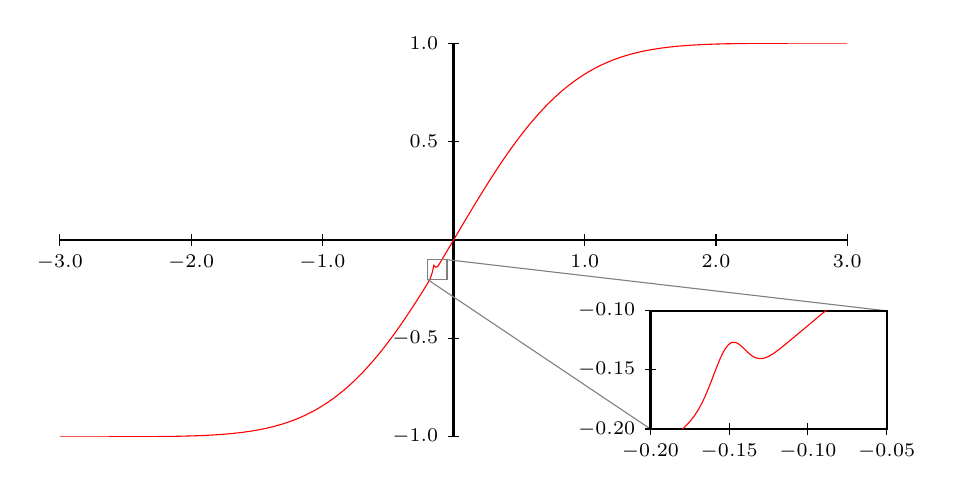
\begin{tikzpicture}[]
\begin{scope}[shift={(0.0,0.0)}]
\pgfsetxvec{\pgfpoint{1.6666666666666667cm}{0cm}}
\pgfsetyvec{\pgfpoint{0cm}{2.5cm}}
\begin{scope}[shift={(3.0,1.0)}]
\begin{scope}[thick,black,fill=white]
\pgfpathmoveto{ \pgfpointxy {-3.0} {0.0}}
\pgfpathlineto{ \pgfpointxy {3.0} {0.0}}
\pgfpathmoveto{ \pgfpointxy {0.0} {-1.0}}
\pgfpathlineto{ \pgfpointxy {0.0} {1.0}}
\pgfusepath{ stroke, }
\end{scope}
\begin{scope}[yshift=2.5cm]
\draw[] [shift={(-3.0,-1.0)}] (0,2pt) -- (0,-2pt) node[below]{ \scriptsize{\num[round-mode=places,round-precision=1]{-3.0}}};
\draw[] [shift={(-2.0,-1.0)}] (0,2pt) -- (0,-2pt) node[below]{ \scriptsize{\num[round-mode=places,round-precision=1]{-2.0}}};
\draw[] [shift={(-1.0,-1.0)}] (0,2pt) -- (0,-2pt) node[below]{ \scriptsize{\num[round-mode=places,round-precision=1]{-1.0}}};
\draw[] [shift={(1.0,-1.0)}] (0,2pt) -- (0,-2pt) node[below]{ \scriptsize{\num[round-mode=places,round-precision=1]{1.0}}};
\draw[] [shift={(2.0,-1.0)}] (0,2pt) -- (0,-2pt) node[below]{ \scriptsize{\num[round-mode=places,round-precision=1]{2.0}}};
\draw[] [shift={(3.0,-1.0)}] (0,2pt) -- (0,-2pt) node[below]{ \scriptsize{\num[round-mode=places,round-precision=1]{3.0}}};
\end{scope}
\begin{scope}[xshift=5.0cm]
\draw[] [shift={(-3.0,-1.0)}] (2pt,0) -- (-2pt,0) node[left]{ \scriptsize{\num[round-mode=places,round-precision=1]{-1.0}}};
\draw[] [shift={(-3.0,-0.5)}] (2pt,0) -- (-2pt,0) node[left]{ \scriptsize{\num[round-mode=places,round-precision=1]{-0.5}}};
\draw[] [shift={(-3.0,0.5)}] (2pt,0) -- (-2pt,0) node[left]{ \scriptsize{\num[round-mode=places,round-precision=1]{0.5}}};
\draw[] [shift={(-3.0,1.0)}] (2pt,0) -- (-2pt,0) node[left]{ \scriptsize{\num[round-mode=places,round-precision=1]{1.0}}};
\end{scope}
\end{scope}
\pgfsetxvec{\pgfpoint{1cm}{0cm}}
\pgfsetyvec{\pgfpoint{0cm}{1cm}}
\end{scope}
\begin{scope}[]
\pgfpathmoveto{ \pgfpointadd{\pgfpointxy {0.0} {0.0}} {\pgfpoint{0cm}{0cm}} }
\pgfpathlineto{ \pgfpointadd{\pgfpointxy {0.0} {0.0}} {\pgfpoint{10cm}{0cm}} }
\pgfpathlineto{ \pgfpointadd{\pgfpointxy {0.0} {0.0}} {\pgfpoint{10cm}{5cm}} }
\pgfpathlineto{ \pgfpointadd{\pgfpointxy {0.0} {0.0}} {\pgfpoint{0cm}{5cm}} }
\pgfpathclose
\pgfusepath{  clip, }
\begin{scope}[shift={(0.0,0.0)}]
\pgfsetxvec{\pgfpoint{1.6666666666666667cm}{0cm}}
\pgfsetyvec{\pgfpoint{0cm}{2.5cm}}
\begin{scope}[shift={(3.0,1.0)}]
\begin{scope}[red]
\pgfpathmoveto{ \pgfpointxy {-3.0} {-0.9999778948503159}}
\pgfpathlineto{ \pgfpointxy {-2.985} {-0.9999757083515112}}
\pgfpathlineto{ \pgfpointxy {-2.97} {-0.9999733170632894}}
\pgfpathlineto{ \pgfpointxy {-2.955} {-0.999970702980543}}
\pgfpathlineto{ \pgfpointxy {-2.94} {-0.9999678466302895}}
\pgfpathlineto{ \pgfpointxy {-2.925} {-0.9999647269627512}}
\pgfpathlineto{ \pgfpointxy {-2.91} {-0.9999613212353085}}
\pgfpathlineto{ \pgfpointxy {-2.895} {-0.9999576048889374}}
\pgfpathlineto{ \pgfpointxy {-2.88} {-0.9999535514167339}}
\pgfpathlineto{ \pgfpointxy {-2.865} {-0.9999491322241092}}
\pgfpathlineto{ \pgfpointxy {-2.85} {-0.9999443164802247}}
\pgfpathlineto{ \pgfpointxy {-2.835} {-0.9999390709602284}}
\pgfpathlineto{ \pgfpointxy {-2.82} {-0.9999333598778289}}
\pgfpathlineto{ \pgfpointxy {-2.805} {-0.9999271447077411}}
\pgfpathlineto{ \pgfpointxy {-2.79} {-0.9999203839975161}}
\pgfpathlineto{ \pgfpointxy {-2.775} {-0.9999130331682573}}
\pgfpathlineto{ \pgfpointxy {-2.76} {-0.9999050443037141}}
\pgfpathlineto{ \pgfpointxy {-2.745} {-0.9998963659272275}}
\pgfpathlineto{ \pgfpointxy {-2.73} {-0.9998869427659972}}
\pgfpathlineto{ \pgfpointxy {-2.715} {-0.9998767155021218}}
\pgfpathlineto{ \pgfpointxy {-2.7} {-0.9998656205098599}}
\pgfpathlineto{ \pgfpointxy {-2.685} {-0.9998535895785484}}
\pgfpathlineto{ \pgfpointxy {-2.67} {-0.9998405496206055}}
\pgfpathlineto{ \pgfpointxy {-2.6550000000000002} {-0.9998264223640424}}
\pgfpathlineto{ \pgfpointxy {-2.64} {-0.9998111240288999}}
\pgfpathlineto{ \pgfpointxy {-2.625} {-0.9997945649870237}}
\pgfpathlineto{ \pgfpointxy {-2.61} {-0.9997766494045888}}
\pgfpathlineto{ \pgfpointxy {-2.595} {-0.9997572748667864}}
\pgfpathlineto{ \pgfpointxy {-2.58} {-0.999736331984083}}
\pgfpathlineto{ \pgfpointxy {-2.565} {-0.9997137039794691}}
\pgfpathlineto{ \pgfpointxy {-2.55} {-0.9996892662561212}}
\pgfpathlineto{ \pgfpointxy {-2.535} {-0.9996628859449036}}
\pgfpathlineto{ \pgfpointxy {-2.52} {-0.9996344214311546}}
\pgfpathlineto{ \pgfpointxy {-2.505} {-0.9996037218602093}}
\pgfpathlineto{ \pgfpointxy {-2.49} {-0.9995706266211303}}
\pgfpathlineto{ \pgfpointxy {-2.475} {-0.9995349648081364}}
\pgfpathlineto{ \pgfpointxy {-2.46} {-0.9994965546592407}}
\pgfpathlineto{ \pgfpointxy {-2.4450000000000003} {-0.9994552029716378}}
\pgfpathlineto{ \pgfpointxy {-2.43} {-0.9994107044934063}}
\pgfpathlineto{ \pgfpointxy {-2.415} {-0.9993628412911277}}
\pgfpathlineto{ \pgfpointxy {-2.4} {-0.99931138209306}}
\pgfpathlineto{ \pgfpointxy {-2.385} {-0.9992560816075419}}
\pgfpathlineto{ \pgfpointxy {-2.37} {-0.9991966798163542}}
\pgfpathlineto{ \pgfpointxy {-2.355} {-0.999132901242809}}
\pgfpathlineto{ \pgfpointxy {-2.34} {-0.9990644541943925}}
\pgfpathlineto{ \pgfpointxy {-2.325} {-0.9989910299798491}}
\pgfpathlineto{ \pgfpointxy {-2.31} {-0.9989123021006515}}
\pgfpathlineto{ \pgfpointxy {-2.295} {-0.9988279254168742}}
\pgfpathlineto{ \pgfpointxy {-2.2800000000000002} {-0.9987375352875576}}
\pgfpathlineto{ \pgfpointxy {-2.265} {-0.9986407466857308}}
\pgfpathlineto{ \pgfpointxy {-2.25} {-0.9985371532883388}}
\pgfpathlineto{ \pgfpointxy {-2.235} {-0.9984263265414133}}
\pgfpathlineto{ \pgfpointxy {-2.2199999999999998} {-0.9983078147009155}}
\pgfpathlineto{ \pgfpointxy {-2.205} {-0.9981811418497791}}
\pgfpathlineto{ \pgfpointxy {-2.19} {-0.9980458068917848}}
\pgfpathlineto{ \pgfpointxy {-2.175} {-0.9979012825230041}}
\pgfpathlineto{ \pgfpointxy {-2.16} {-0.9977470141816697}}
\pgfpathlineto{ \pgfpointxy {-2.145} {-0.997582418977438}}
\pgfpathlineto{ \pgfpointxy {-2.13} {-0.9974068846011453}}
\pgfpathlineto{ \pgfpointxy {-2.115} {-0.997219768216276}}
\pgfpathlineto{ \pgfpointxy {-2.1} {-0.9970203953335013}}
\pgfpathlineto{ \pgfpointxy {-2.085} {-0.9968080586697832}}
\pgfpathlineto{ \pgfpointxy {-2.0700000000000003} {-0.9965820169936752}}
\pgfpathlineto{ \pgfpointxy {-2.055} {-0.9963414939586048}}
\pgfpathlineto{ \pgfpointxy {-2.04} {-0.9960856769260644}}
\pgfpathlineto{ \pgfpointxy {-2.025} {-0.9958137157807956}}
\pgfpathlineto{ \pgfpointxy {-2.01} {-0.9955247217402033}}
\pgfpathlineto{ \pgfpointxy {-1.995} {-0.9952177661603995}}
\pgfpathlineto{ \pgfpointxy {-1.98} {-0.9948918793414291}}
\pgfpathlineto{ \pgfpointxy {-1.965} {-0.9945460493344039}}
\pgfpathlineto{ \pgfpointxy {-1.95} {-0.9941792207534235}}
\pgfpathlineto{ \pgfpointxy {-1.935} {-0.9937902935953322}}
\pgfpathlineto{ \pgfpointxy {-1.92} {-0.9933781220705278}}
\pgfpathlineto{ \pgfpointxy {-1.905} {-0.992941513448194}}
\pgfpathlineto{ \pgfpointxy {-1.8900000000000001} {-0.9924792269195024}}
\pgfpathlineto{ \pgfpointxy {-1.875} {-0.9919899724824818}}
\pgfpathlineto{ \pgfpointxy {-1.86} {-0.9914724098524189}}
\pgfpathlineto{ \pgfpointxy {-1.845} {-0.9909251474018062}}
\pgfpathlineto{ \pgfpointxy {-1.83} {-0.9903467411340076}}
\pgfpathlineto{ \pgfpointxy {-1.815} {-0.9897356936949588}}
\pgfpathlineto{ \pgfpointxy {-1.8} {-0.9890904534273609}}
\pgfpathlineto{ \pgfpointxy {-1.7850000000000001} {-0.9884094134719639}}
\pgfpathlineto{ \pgfpointxy {-1.77} {-0.9876909109206615}}
\pgfpathlineto{ \pgfpointxy {-1.7550000000000001} {-0.9869332260262446}}
\pgfpathlineto{ \pgfpointxy {-1.74} {-0.9861345814737644}}
\pgfpathlineto{ \pgfpointxy {-1.725} {-0.9852931417185677}}
\pgfpathlineto{ \pgfpointxy {-1.71} {-0.9844070123961483}}
\pgfpathlineto{ \pgfpointxy {-1.695} {-0.9834742398090428}}
\pgfpathlineto{ \pgfpointxy {-1.6800000000000002} {-0.9824928104960676}}
\pgfpathlineto{ \pgfpointxy {-1.665} {-0.9814606508892384}}
\pgfpathlineto{ \pgfpointxy {-1.6500000000000001} {-0.9803756270637614}}
\pgfpathlineto{ \pgfpointxy {-1.635} {-0.9792355445865027}}
\pgfpathlineto{ \pgfpointxy {-1.62} {-0.9780381484683515}}
\pgfpathlineto{ \pgfpointxy {-1.605} {-0.9767811232258793}}
\pgfpathlineto{ \pgfpointxy {-1.59} {-0.9754620930576753}}
\pgfpathlineto{ \pgfpointxy {-1.575} {-0.9740786221406821}}
\pgfpathlineto{ \pgfpointxy {-1.56} {-0.9726282150517984}}
\pgfpathlineto{ \pgfpointxy {-1.5450000000000002} {-0.97110831731992}}
\pgfpathlineto{ \pgfpointxy {-1.53} {-0.9695163161134889}}
\pgfpathlineto{ \pgfpointxy {-1.5150000000000001} {-0.9678495410684881}}
\pgfpathlineto{ \pgfpointxy {-1.5} {-0.9661052652616654}}
\pgfpathlineto{ \pgfpointxy {-1.485} {-0.9642807063336017}}
\pgfpathlineto{ \pgfpointxy {-1.47} {-0.9623730277660346}}
\pgfpathlineto{ \pgfpointxy {-1.455} {-0.9603793403176331}}
\pgfpathlineto{ \pgfpointxy {-1.44} {-0.958296703622169}}
\pgfpathlineto{ \pgfpointxy {-1.425} {-0.9561221279527699}}
\pgfpathlineto{ \pgfpointxy {-1.4100000000000001} {-0.9538525761556357}}
\pgfpathlineto{ \pgfpointxy {-1.395} {-0.9514849657562949}}
\pgfpathlineto{ \pgfpointxy {-1.3800000000000001} {-0.9490161712411282}}
\pgfpathlineto{ \pgfpointxy {-1.365} {-0.9464430265165276}}
\pgfpathlineto{ \pgfpointxy {-1.35} {-0.943762327547669}}
\pgfpathlineto{ \pgfpointxy {-1.335} {-0.9409708351784686}}
\pgfpathlineto{ \pgfpointxy {-1.32} {-0.9380652781338571}}
\pgfpathlineto{ \pgfpointxy {-1.3050000000000002} {-0.9350423562050534}}
\pgfpathlineto{ \pgfpointxy {-1.29} {-0.9318987436180433}}
\pgfpathlineto{ \pgfpointxy {-1.2750000000000001} {-0.9286310925849711}}
\pgfpathlineto{ \pgfpointxy {-1.26} {-0.92523603703764}}
\pgfpathlineto{ \pgfpointxy {-1.245} {-0.92171019654178}}
\pgfpathlineto{ \pgfpointxy {-1.23} {-0.9180501803901957}}
\pgfpathlineto{ \pgfpointxy {-1.215} {-0.9142525918723391}}
\pgfpathlineto{ \pgfpointxy {-1.2000000000000002} {-0.910314032717273}}
\pgfpathlineto{ \pgfpointxy {-1.185} {-0.9062311077063987}}
\pgfpathlineto{ \pgfpointxy {-1.1700000000000002} {-0.9020004294517225}}
\pgfpathlineto{ \pgfpointxy {-1.155} {-0.8976186233348172}}
\pgfpathlineto{ \pgfpointxy {-1.1400000000000001} {-0.8930823326010242}}
\pgfpathlineto{ \pgfpointxy {-1.125} {-0.8883882236028127}}
\pgfpathlineto{ \pgfpointxy {-1.11} {-0.8835329911855913}}
\pgfpathlineto{ \pgfpointxy {-1.095} {-0.8785133642086344}}
\pgfpathlineto{ \pgfpointxy {-1.08} {-0.8733261111931682}}
\pgfpathlineto{ \pgfpointxy {-1.0650000000000002} {-0.867968046089032}}
\pgfpathlineto{ \pgfpointxy {-1.05} {-0.8624360341507235}}
\pgfpathlineto{ \pgfpointxy {-1.0350000000000001} {-0.8567269979130236}}
\pgfpathlineto{ \pgfpointxy {-1.02} {-0.8508379232558065}}
\pgfpathlineto{ \pgfpointxy {-1.0050000000000001} {-0.8447658655470591}}
\pgfpathlineto{ \pgfpointxy {-0.9900000000000002} {-0.8385079558525668}}
\pgfpathlineto{ \pgfpointxy {-0.9750000000000001} {-0.83206140720018}}
\pgfpathlineto{ \pgfpointxy {-0.96} {-0.8254235208860544}}
\pgfpathlineto{ \pgfpointxy {-0.9450000000000003} {-0.81859169280975}}
\pgfpathlineto{ \pgfpointxy {-0.9300000000000002} {-0.8115634198246098}}
\pgfpathlineto{ \pgfpointxy {-0.915} {-0.8043363060893939}}
\pgfpathlineto{ \pgfpointxy {-0.8999999999999999} {-0.7969080694067268}}
\pgfpathlineto{ \pgfpointxy {-0.8850000000000002} {-0.7892765475335458}}
\pgfpathlineto{ \pgfpointxy {-0.8700000000000001} {-0.7814397044483927}}
\pgfpathlineto{ \pgfpointxy {-0.855} {-0.7733956365600895}}
\pgfpathlineto{ \pgfpointxy {-0.8399999999999999} {-0.7651425788420778}}
\pgfpathlineto{ \pgfpointxy {-0.8250000000000002} {-0.7566789108764818}}
\pgfpathlineto{ \pgfpointxy {-0.81} {-0.7480031627917798}}
\pgfpathlineto{ \pgfpointxy {-0.7949999999999999} {-0.7391140210778491}}
\pgfpathlineto{ \pgfpointxy {-0.7800000000000002} {-0.7300103342620572}}
\pgfpathlineto{ \pgfpointxy {-0.7650000000000001} {-0.720691118430056}}
\pgfpathlineto{ \pgfpointxy {-0.75} {-0.7111555625749495}}
\pgfpathlineto{ \pgfpointxy {-0.7349999999999999} {-0.7014030337585848}}
\pgfpathlineto{ \pgfpointxy {-0.7200000000000002} {-0.6914330820688371}}
\pgfpathlineto{ \pgfpointxy {-0.7050000000000001} {-0.6812454453569445}}
\pgfpathlineto{ \pgfpointxy {-0.69} {-0.670840053739193}}
\pgfpathlineto{ \pgfpointxy {-0.6750000000000003} {-0.6602170338475166}}
\pgfpathlineto{ \pgfpointxy {-0.6600000000000001} {-0.6493767128139546}}
\pgfpathlineto{ \pgfpointxy {-0.645} {-0.6383196219742868}}
\pgfpathlineto{ \pgfpointxy {-0.6299999999999999} {-0.6270465002766268}}
\pgfpathlineto{ \pgfpointxy {-0.6150000000000002} {-0.6155582973812643}}
\pgfpathlineto{ \pgfpointxy {-0.6000000000000001} {-0.6038561764386106}}
\pgfpathlineto{ \pgfpointxy {-0.585} {-0.5919415165327075}}
\pgfpathlineto{ \pgfpointxy {-0.5700000000000003} {-0.5798159147784314}}
\pgfpathlineto{ \pgfpointxy {-0.5550000000000002} {-0.56748118806123}}
\pgfpathlineto{ \pgfpointxy {-0.54} {-0.5549393744090031}}
\pgfpathlineto{ \pgfpointxy {-0.5249999999999999} {-0.5421927339865252}}
\pgfpathlineto{ \pgfpointxy {-0.5100000000000002} {-0.5292437497036775}}
\pgfpathlineto{ \pgfpointxy {-0.4950000000000001} {-0.5160951274296337}}
\pgfpathlineto{ \pgfpointxy {-0.48} {-0.5027497958060796}}
\pgfpathlineto{ \pgfpointxy {-0.4650000000000003} {-0.4892109056535041}}
\pgfpathlineto{ \pgfpointxy {-0.4500000000000002} {-0.4754818289656054}}
\pgfpathlineto{ \pgfpointxy {-0.43500000000000005} {-0.46156615748787366}}
\pgfpathlineto{ \pgfpointxy {-0.41999999999999993} {-0.4474677008774629}}
\pgfpathlineto{ \pgfpointxy {-0.40500000000000025} {-0.43319048444254893}}
\pgfpathlineto{ \pgfpointxy {-0.3900000000000001} {-0.4187387464604462}}
\pgfpathlineto{ \pgfpointxy {-0.375} {-0.40411693507488256}}
\pgfpathlineto{ \pgfpointxy {-0.3600000000000003} {-0.38932970477393625}}
\pgfpathlineto{ \pgfpointxy {-0.3450000000000002} {-0.37438191245126506}}
\pgfpathlineto{ \pgfpointxy {-0.33000000000000007} {-0.3592786130544001}}
\pgfpathlineto{ \pgfpointxy {-0.31499999999999995} {-0.3440250548249846}}
\pgfpathlineto{ \pgfpointxy {-0.30000000000000027} {-0.3286266741369791}}
\pgfpathlineto{ \pgfpointxy {-0.28500000000000014} {-0.31308908993994433}}
\pgfpathlineto{ \pgfpointxy {-0.27} {-0.2974180978156481}}
\pgfpathlineto{ \pgfpointxy {-0.2549999999999999} {-0.2816196636572761}}
\pgfpathlineto{ \pgfpointxy {-0.2400000000000002} {-0.2656999169816263}}
\pgfpathlineto{ \pgfpointxy {-0.2250000000000001} {-0.24966514388565572}}
\pgfpathlineto{ \pgfpointxy {-0.20999999999999996} {-0.23352177905236451}}
\pgfpathlineto{ \pgfpointxy {-0.19500000000000028} {-0.2172748026978713}}
\pgfpathlineto{ \pgfpointxy {-0.18000000000000016} {-0.20049253349307294}}
\pgfpathlineto{ \pgfpointxy {-0.16500000000000004} {-0.171554807205249}}
\pgfpathlineto{ \pgfpointxy {-0.1499999999999999} {-0.12810167016535548}}
\pgfpathlineto{ \pgfpointxy {-0.13500000000000023} {-0.13845901250096762}}
\pgfpathlineto{ \pgfpointxy {-0.1200000000000001} {-0.13431516142643635}}
\pgfpathlineto{ \pgfpointxy {-0.10499999999999998} {-0.11804426945267814}}
\pgfpathlineto{ \pgfpointxy {-0.0900000000000003} {-0.10128066269133476}}
\pgfpathlineto{ \pgfpointxy {-0.07500000000000018} {-0.08447012899878711}}
\pgfpathlineto{ \pgfpointxy {-0.06000000000000005} {-0.06762172105686759}}
\pgfpathlineto{ \pgfpointxy {-0.04499999999999993} {-0.050742945320982}}
\pgfpathlineto{ \pgfpointxy {-0.03000000000000025} {-0.03384134712627562}}
\pgfpathlineto{ \pgfpointxy {-0.015000000000000124} {-0.016924500953862887}}
\pgfpathlineto{ \pgfpointxy {0.0} {0.000000000000000000000000000000000000000000000000005530709549844417}}
\pgfpathlineto{ \pgfpointxy {0.01499999999999968} {0.01692450095386222}}
\pgfpathlineto{ \pgfpointxy {0.029999999999999805} {0.03384134712627496}}
\pgfpathlineto{ \pgfpointxy {0.04499999999999993} {0.050742945320982}}
\pgfpathlineto{ \pgfpointxy {0.06000000000000005} {0.06762172105686759}}
\pgfpathlineto{ \pgfpointxy {0.07499999999999973} {0.08447012899881046}}
\pgfpathlineto{ \pgfpointxy {0.08999999999999986} {0.10128066329892249}}
\pgfpathlineto{ \pgfpointxy {0.10499999999999998} {0.11804586782678883}}
\pgfpathlineto{ \pgfpointxy {0.1200000000000001} {0.13475834626763017}}
\pgfpathlineto{ \pgfpointxy {0.1349999999999998} {0.1514107720675565}}
\pgfpathlineto{ \pgfpointxy {0.1499999999999999} {0.16799589820549876}}
\pgfpathlineto{ \pgfpointxy {0.16500000000000004} {0.18450656677183808}}
\pgfpathlineto{ \pgfpointxy {0.17999999999999972} {0.20093571833426616}}
\pgfpathlineto{ \pgfpointxy {0.19499999999999984} {0.21727640107198132}}
\pgfpathlineto{ \pgfpointxy {0.20999999999999996} {0.2335217796599528}}
\pgfpathlineto{ \pgfpointxy {0.2250000000000001} {0.24966514388568006}}
\pgfpathlineto{ \pgfpointxy {0.23999999999999977} {0.26569991698162565}}
\pgfpathlineto{ \pgfpointxy {0.2549999999999999} {0.2816196636572761}}
\pgfpathlineto{ \pgfpointxy {0.27} {0.2974180978156481}}
\pgfpathlineto{ \pgfpointxy {0.2849999999999997} {0.31308908993994355}}
\pgfpathlineto{ \pgfpointxy {0.2999999999999998} {0.32862667413697844}}
\pgfpathlineto{ \pgfpointxy {0.31499999999999995} {0.3440250548249846}}
\pgfpathlineto{ \pgfpointxy {0.33000000000000007} {0.3592786130544001}}
\pgfpathlineto{ \pgfpointxy {0.34499999999999975} {0.3743819124512646}}
\pgfpathlineto{ \pgfpointxy {0.3599999999999999} {0.3893297047739359}}
\pgfpathlineto{ \pgfpointxy {0.375} {0.40411693507488256}}
\pgfpathlineto{ \pgfpointxy {0.3899999999999997} {0.4187387464604456}}
\pgfpathlineto{ \pgfpointxy {0.4049999999999998} {0.4331904844425486}}
\pgfpathlineto{ \pgfpointxy {0.41999999999999993} {0.4474677008774629}}
\pgfpathlineto{ \pgfpointxy {0.43500000000000005} {0.46156615748787366}}
\pgfpathlineto{ \pgfpointxy {0.44999999999999973} {0.47548182896560476}}
\pgfpathlineto{ \pgfpointxy {0.46499999999999986} {0.48921090565350367}}
\pgfpathlineto{ \pgfpointxy {0.48} {0.5027497958060796}}
\pgfpathlineto{ \pgfpointxy {0.49499999999999966} {0.5160951274296333}}
\pgfpathlineto{ \pgfpointxy {0.5099999999999998} {0.529243749703677}}
\pgfpathlineto{ \pgfpointxy {0.5249999999999999} {0.5421927339865252}}
\pgfpathlineto{ \pgfpointxy {0.54} {0.5549393744090031}}
\pgfpathlineto{ \pgfpointxy {0.5549999999999997} {0.5674811880612298}}
\pgfpathlineto{ \pgfpointxy {0.5699999999999998} {0.5798159147784312}}
\pgfpathlineto{ \pgfpointxy {0.585} {0.5919415165327075}}
\pgfpathlineto{ \pgfpointxy {0.5999999999999996} {0.6038561764386103}}
\pgfpathlineto{ \pgfpointxy {0.6149999999999998} {0.6155582973812639}}
\pgfpathlineto{ \pgfpointxy {0.6299999999999999} {0.6270465002766268}}
\pgfpathlineto{ \pgfpointxy {0.645} {0.6383196219742868}}
\pgfpathlineto{ \pgfpointxy {0.6599999999999997} {0.6493767128139543}}
\pgfpathlineto{ \pgfpointxy {0.6749999999999998} {0.6602170338475164}}
\pgfpathlineto{ \pgfpointxy {0.69} {0.670840053739193}}
\pgfpathlineto{ \pgfpointxy {0.7050000000000001} {0.6812454453569445}}
\pgfpathlineto{ \pgfpointxy {0.7199999999999998} {0.6914330820688368}}
\pgfpathlineto{ \pgfpointxy {0.7349999999999999} {0.7014030337585848}}
\pgfpathlineto{ \pgfpointxy {0.75} {0.7111555625749495}}
\pgfpathlineto{ \pgfpointxy {0.7649999999999997} {0.7206911184300557}}
\pgfpathlineto{ \pgfpointxy {0.7799999999999998} {0.730010334262057}}
\pgfpathlineto{ \pgfpointxy {0.7949999999999999} {0.7391140210778491}}
\pgfpathlineto{ \pgfpointxy {0.81} {0.7480031627917798}}
\pgfpathlineto{ \pgfpointxy {0.8249999999999997} {0.7566789108764814}}
\pgfpathlineto{ \pgfpointxy {0.8399999999999999} {0.7651425788420778}}
\pgfpathlineto{ \pgfpointxy {0.855} {0.7733956365600895}}
\pgfpathlineto{ \pgfpointxy {0.8699999999999997} {0.7814397044483924}}
\pgfpathlineto{ \pgfpointxy {0.8849999999999998} {0.7892765475335456}}
\pgfpathlineto{ \pgfpointxy {0.8999999999999999} {0.7969080694067268}}
\pgfpathlineto{ \pgfpointxy {0.915} {0.8043363060893939}}
\pgfpathlineto{ \pgfpointxy {0.9299999999999997} {0.8115634198246096}}
\pgfpathlineto{ \pgfpointxy {0.9449999999999998} {0.8185916928097499}}
\pgfpathlineto{ \pgfpointxy {0.96} {0.8254235208860544}}
\pgfpathlineto{ \pgfpointxy {0.9749999999999996} {0.8320614072001797}}
\pgfpathlineto{ \pgfpointxy {0.9899999999999998} {0.8385079558525665}}
\pgfpathlineto{ \pgfpointxy {1.005} {0.8447658655470591}}
\pgfpathlineto{ \pgfpointxy {1.0199999999999996} {0.8508379232558063}}
\pgfpathlineto{ \pgfpointxy {1.0350000000000001} {0.8567269979130236}}
\pgfpathlineto{ \pgfpointxy {1.0499999999999998} {0.8624360341507233}}
\pgfpathlineto{ \pgfpointxy {1.0649999999999995} {0.8679680460890318}}
\pgfpathlineto{ \pgfpointxy {1.08} {0.8733261111931682}}
\pgfpathlineto{ \pgfpointxy {1.0949999999999998} {0.8785133642086344}}
\pgfpathlineto{ \pgfpointxy {1.1099999999999994} {0.883532991185591}}
\pgfpathlineto{ \pgfpointxy {1.125} {0.8883882236028127}}
\pgfpathlineto{ \pgfpointxy {1.1399999999999997} {0.893082332601024}}
\pgfpathlineto{ \pgfpointxy {1.1550000000000002} {0.8976186233348173}}
\pgfpathlineto{ \pgfpointxy {1.17} {0.9020004294517224}}
\pgfpathlineto{ \pgfpointxy {1.1849999999999996} {0.9062311077063985}}
\pgfpathlineto{ \pgfpointxy {1.2000000000000002} {0.910314032717273}}
\pgfpathlineto{ \pgfpointxy {1.2149999999999999} {0.9142525918723391}}
\pgfpathlineto{ \pgfpointxy {1.2299999999999995} {0.9180501803901956}}
\pgfpathlineto{ \pgfpointxy {1.245} {0.92171019654178}}
\pgfpathlineto{ \pgfpointxy {1.2599999999999998} {0.9252360370376399}}
\pgfpathlineto{ \pgfpointxy {1.2749999999999995} {0.928631092584971}}
\pgfpathlineto{ \pgfpointxy {1.29} {0.9318987436180433}}
\pgfpathlineto{ \pgfpointxy {1.3049999999999997} {0.9350423562050534}}
\pgfpathlineto{ \pgfpointxy {1.3200000000000003} {0.9380652781338571}}
\pgfpathlineto{ \pgfpointxy {1.335} {0.9409708351784686}}
\pgfpathlineto{ \pgfpointxy {1.3499999999999996} {0.943762327547669}}
\pgfpathlineto{ \pgfpointxy {1.3650000000000002} {0.9464430265165277}}
\pgfpathlineto{ \pgfpointxy {1.38} {0.9490161712411282}}
\pgfpathlineto{ \pgfpointxy {1.3949999999999996} {0.9514849657562948}}
\pgfpathlineto{ \pgfpointxy {1.4100000000000001} {0.9538525761556357}}
\pgfpathlineto{ \pgfpointxy {1.4249999999999998} {0.9561221279527699}}
\pgfpathlineto{ \pgfpointxy {1.4399999999999995} {0.9582967036221689}}
\pgfpathlineto{ \pgfpointxy {1.455} {0.9603793403176331}}
\pgfpathlineto{ \pgfpointxy {1.4699999999999998} {0.9623730277660346}}
\pgfpathlineto{ \pgfpointxy {1.4849999999999994} {0.9642807063336016}}
\pgfpathlineto{ \pgfpointxy {1.5} {0.9661052652616654}}
\pgfpathlineto{ \pgfpointxy {1.5149999999999997} {0.967849541068488}}
\pgfpathlineto{ \pgfpointxy {1.5300000000000002} {0.969516316113489}}
\pgfpathlineto{ \pgfpointxy {1.545} {0.9711083173199199}}
\pgfpathlineto{ \pgfpointxy {1.5599999999999996} {0.9726282150517984}}
\pgfpathlineto{ \pgfpointxy {1.5750000000000002} {0.9740786221406821}}
\pgfpathlineto{ \pgfpointxy {1.5899999999999999} {0.9754620930576752}}
\pgfpathlineto{ \pgfpointxy {1.6049999999999995} {0.9767811232258793}}
\pgfpathlineto{ \pgfpointxy {1.62} {0.9780381484683515}}
\pgfpathlineto{ \pgfpointxy {1.6349999999999998} {0.9792355445865027}}
\pgfpathlineto{ \pgfpointxy {1.6499999999999995} {0.9803756270637612}}
\pgfpathlineto{ \pgfpointxy {1.665} {0.9814606508892384}}
\pgfpathlineto{ \pgfpointxy {1.6799999999999997} {0.9824928104960676}}
\pgfpathlineto{ \pgfpointxy {1.6949999999999994} {0.9834742398090427}}
\pgfpathlineto{ \pgfpointxy {1.71} {0.9844070123961483}}
\pgfpathlineto{ \pgfpointxy {1.7249999999999996} {0.9852931417185677}}
\pgfpathlineto{ \pgfpointxy {1.7400000000000002} {0.9861345814737644}}
\pgfpathlineto{ \pgfpointxy {1.755} {0.9869332260262446}}
\pgfpathlineto{ \pgfpointxy {1.7699999999999996} {0.9876909109206615}}
\pgfpathlineto{ \pgfpointxy {1.7850000000000001} {0.9884094134719639}}
\pgfpathlineto{ \pgfpointxy {1.7999999999999998} {0.9890904534273609}}
\pgfpathlineto{ \pgfpointxy {1.8149999999999995} {0.9897356936949588}}
\pgfpathlineto{ \pgfpointxy {1.83} {0.9903467411340076}}
\pgfpathlineto{ \pgfpointxy {1.8449999999999998} {0.9909251474018062}}
\pgfpathlineto{ \pgfpointxy {1.8599999999999994} {0.9914724098524188}}
\pgfpathlineto{ \pgfpointxy {1.875} {0.9919899724824818}}
\pgfpathlineto{ \pgfpointxy {1.8899999999999997} {0.9924792269195024}}
\pgfpathlineto{ \pgfpointxy {1.9050000000000002} {0.992941513448194}}
\pgfpathlineto{ \pgfpointxy {1.92} {0.9933781220705278}}
\pgfpathlineto{ \pgfpointxy {1.9349999999999996} {0.9937902935953322}}
\pgfpathlineto{ \pgfpointxy {1.9500000000000002} {0.9941792207534235}}
\pgfpathlineto{ \pgfpointxy {1.9649999999999999} {0.9945460493344039}}
\pgfpathlineto{ \pgfpointxy {1.9799999999999995} {0.9948918793414291}}
\pgfpathlineto{ \pgfpointxy {1.995} {0.9952177661603995}}
\pgfpathlineto{ \pgfpointxy {2.01} {0.9955247217402033}}
\pgfpathlineto{ \pgfpointxy {2.0249999999999995} {0.9958137157807956}}
\pgfpathlineto{ \pgfpointxy {2.04} {0.9960856769260644}}
\pgfpathlineto{ \pgfpointxy {2.0549999999999997} {0.9963414939586048}}
\pgfpathlineto{ \pgfpointxy {2.0699999999999994} {0.9965820169936752}}
\pgfpathlineto{ \pgfpointxy {2.085} {0.9968080586697832}}
\pgfpathlineto{ \pgfpointxy {2.0999999999999996} {0.9970203953335013}}
\pgfpathlineto{ \pgfpointxy {2.115} {0.997219768216276}}
\pgfpathlineto{ \pgfpointxy {2.13} {0.9974068846011453}}
\pgfpathlineto{ \pgfpointxy {2.1449999999999996} {0.997582418977438}}
\pgfpathlineto{ \pgfpointxy {2.16} {0.9977470141816697}}
\pgfpathlineto{ \pgfpointxy {2.175} {0.9979012825230041}}
\pgfpathlineto{ \pgfpointxy {2.1899999999999995} {0.9980458068917848}}
\pgfpathlineto{ \pgfpointxy {2.205} {0.9981811418497791}}
\pgfpathlineto{ \pgfpointxy {2.2199999999999998} {0.9983078147009155}}
\pgfpathlineto{ \pgfpointxy {2.2349999999999994} {0.9984263265414133}}
\pgfpathlineto{ \pgfpointxy {2.25} {0.9985371532883388}}
\pgfpathlineto{ \pgfpointxy {2.2649999999999997} {0.9986407466857308}}
\pgfpathlineto{ \pgfpointxy {2.2799999999999994} {0.9987375352875576}}
\pgfpathlineto{ \pgfpointxy {2.295} {0.9988279254168742}}
\pgfpathlineto{ \pgfpointxy {2.3099999999999996} {0.9989123021006515}}
\pgfpathlineto{ \pgfpointxy {2.325} {0.9989910299798491}}
\pgfpathlineto{ \pgfpointxy {2.34} {0.9990644541943925}}
\pgfpathlineto{ \pgfpointxy {2.3549999999999995} {0.999132901242809}}
\pgfpathlineto{ \pgfpointxy {2.37} {0.9991966798163542}}
\pgfpathlineto{ \pgfpointxy {2.385} {0.9992560816075419}}
\pgfpathlineto{ \pgfpointxy {2.3999999999999995} {0.99931138209306}}
\pgfpathlineto{ \pgfpointxy {2.415} {0.9993628412911277}}
\pgfpathlineto{ \pgfpointxy {2.4299999999999997} {0.9994107044934063}}
\pgfpathlineto{ \pgfpointxy {2.4449999999999994} {0.9994552029716378}}
\pgfpathlineto{ \pgfpointxy {2.46} {0.9994965546592407}}
\pgfpathlineto{ \pgfpointxy {2.4749999999999996} {0.9995349648081364}}
\pgfpathlineto{ \pgfpointxy {2.49} {0.9995706266211303}}
\pgfpathlineto{ \pgfpointxy {2.505} {0.9996037218602093}}
\pgfpathlineto{ \pgfpointxy {2.5199999999999996} {0.9996344214311546}}
\pgfpathlineto{ \pgfpointxy {2.535} {0.9996628859449036}}
\pgfpathlineto{ \pgfpointxy {2.55} {0.9996892662561212}}
\pgfpathlineto{ \pgfpointxy {2.5649999999999995} {0.9997137039794691}}
\pgfpathlineto{ \pgfpointxy {2.58} {0.999736331984083}}
\pgfpathlineto{ \pgfpointxy {2.5949999999999998} {0.9997572748667864}}
\pgfpathlineto{ \pgfpointxy {2.6099999999999994} {0.9997766494045888}}
\pgfpathlineto{ \pgfpointxy {2.625} {0.9997945649870237}}
\pgfpathlineto{ \pgfpointxy {2.6399999999999997} {0.9998111240288999}}
\pgfpathlineto{ \pgfpointxy {2.6549999999999994} {0.9998264223640424}}
\pgfpathlineto{ \pgfpointxy {2.67} {0.9998405496206055}}
\pgfpathlineto{ \pgfpointxy {2.6849999999999996} {0.9998535895785484}}
\pgfpathlineto{ \pgfpointxy {2.7} {0.9998656205098599}}
\pgfpathlineto{ \pgfpointxy {2.715} {0.9998767155021218}}
\pgfpathlineto{ \pgfpointxy {2.7299999999999995} {0.9998869427659972}}
\pgfpathlineto{ \pgfpointxy {2.745} {0.9998963659272275}}
\pgfpathlineto{ \pgfpointxy {2.76} {0.9999050443037141}}
\pgfpathlineto{ \pgfpointxy {2.7749999999999995} {0.9999130331682573}}
\pgfpathlineto{ \pgfpointxy {2.79} {0.9999203839975161}}
\pgfpathlineto{ \pgfpointxy {2.8049999999999997} {0.9999271447077411}}
\pgfpathlineto{ \pgfpointxy {2.8199999999999994} {0.9999333598778289}}
\pgfpathlineto{ \pgfpointxy {2.835} {0.9999390709602284}}
\pgfpathlineto{ \pgfpointxy {2.8499999999999996} {0.9999443164802247}}
\pgfpathlineto{ \pgfpointxy {2.865} {0.9999491322241092}}
\pgfpathlineto{ \pgfpointxy {2.88} {0.9999535514167339}}
\pgfpathlineto{ \pgfpointxy {2.8949999999999996} {0.9999576048889374}}
\pgfpathlineto{ \pgfpointxy {2.91} {0.9999613212353085}}
\pgfpathlineto{ \pgfpointxy {2.925} {0.9999647269627512}}
\pgfpathlineto{ \pgfpointxy {2.9399999999999995} {0.9999678466302895}}
\pgfpathlineto{ \pgfpointxy {2.955} {0.999970702980543}}
\pgfpathlineto{ \pgfpointxy {2.9699999999999998} {0.9999733170632894}}
\pgfpathlineto{ \pgfpointxy {2.9849999999999994} {0.9999757083515112}}
\pgfpathlineto{ \pgfpointxy {3.0} {0.9999778948503159}}
\pgfusepath{ stroke, }
\end{scope}
\end{scope}
\pgfsetxvec{\pgfpoint{1cm}{0cm}}
\pgfsetyvec{\pgfpoint{0cm}{1cm}}
\end{scope}
\end{scope}
\begin{scope}[gray]
\begin{scope}[shift={(0.0,0.0)}]
\pgfsetxvec{\pgfpoint{1.6666666666666667cm}{0cm}}
\pgfsetyvec{\pgfpoint{0cm}{2.5cm}}
\begin{scope}[shift={(3.0,1.0)}]
\pgfpathmoveto{ \pgfpointxy {-0.2} {-0.2}}
\pgfpathlineto{ \pgfpointxy {-0.05} {-0.2}}
\pgfpathlineto{ \pgfpointxy {-0.05} {-0.1}}
\pgfpathlineto{ \pgfpointxy {-0.2} {-0.1}}
\pgfpathclose
\end{scope}
\pgfsetxvec{\pgfpoint{1cm}{0cm}}
\pgfsetyvec{\pgfpoint{0cm}{1cm}}
\end{scope}
\pgfusepath{ stroke, }
\pgfseteorule
\begin{scope}[shift={(7.5,0.1)}]
\pgfsetxvec{\pgfpoint{19.999999999999996cm}{0cm}}
\pgfsetyvec{\pgfpoint{0cm}{15.0cm}}
\begin{scope}[shift={(0.2,0.2)}]
\pgfpathmoveto{ \pgfpointxy {-0.2} {-0.2}}
\pgfpathlineto{ \pgfpointxy {-0.05} {-0.2}}
\pgfpathlineto{ \pgfpointxy {-0.05} {-0.1}}
\pgfpathlineto{ \pgfpointxy {-0.2} {-0.1}}
\pgfpathclose
\end{scope}
\pgfsetxvec{\pgfpoint{1cm}{0cm}}
\pgfsetyvec{\pgfpoint{0cm}{1cm}}
\end{scope}
\begin{scope}[shift={(0.0,0.0)}]
\pgfsetxvec{\pgfpoint{1.6666666666666667cm}{0cm}}
\pgfsetyvec{\pgfpoint{0cm}{2.5cm}}
\begin{scope}[shift={(3.0,1.0)}]
\pgfpathmoveto{ \pgfpointxy {-0.2} {-0.2}}
\pgfpathlineto{ \pgfpointxy {-0.05} {-0.2}}
\pgfpathlineto{ \pgfpointxy {-0.05} {-0.1}}
\pgfpathlineto{ \pgfpointxy {-0.2} {-0.1}}
\pgfpathclose
\end{scope}
\pgfsetxvec{\pgfpoint{1cm}{0cm}}
\pgfsetyvec{\pgfpoint{0cm}{1cm}}
\end{scope}
\pgfpathmoveto{ \pgfpointxy {0.0} {0.0}}
\pgfpathlineto{ \pgfpointxy {10.5} {0.0}}
\pgfpathlineto{ \pgfpointxy {10.5} {5.0}}
\pgfpathlineto{ \pgfpointxy {0.0} {5.0}}
\pgfpathclose
\pgfusepath{  clip, }
\pgfpathmoveto{ \pgfpointxy {4.666666666666667} {2.0}}
\pgfpathlineto{ \pgfpointxy {7.5} {0.1}}
\pgfpathmoveto{ \pgfpointxy {4.916666666666667} {2.25}}
\pgfpathlineto{ \pgfpointxy {10.5} {1.6}}
\pgfusepath{ stroke, }
\end{scope}
\begin{scope}[shift={(7.5,0.1)}]
\pgfsetxvec{\pgfpoint{19.999999999999996cm}{0cm}}
\pgfsetyvec{\pgfpoint{0cm}{15.0cm}}
\begin{scope}[shift={(0.2,0.2)}]
\begin{scope}[thick,black,fill=white]
\pgfpathmoveto{ \pgfpointxy {-0.2} {-0.2}}
\pgfpathlineto{ \pgfpointxy {-0.05} {-0.2}}
\pgfpathlineto{ \pgfpointxy {-0.05} {-0.1}}
\pgfpathlineto{ \pgfpointxy {-0.2} {-0.1}}
\pgfpathclose
\pgfusepath{ stroke, fill, }
\end{scope}
\begin{scope}[yshift=0cm]
\draw[] [shift={(-0.2,-0.2)}] (0,2pt) -- (0,-2pt) node[below]{ \scriptsize{\num[round-mode=places,round-precision=2]{-0.2}}};
\draw[] [shift={(-0.15000000000000002,-0.2)}] (0,2pt) -- (0,-2pt) node[below]{ \scriptsize{\num[round-mode=places,round-precision=2]{-0.15000000000000002}}};
\draw[] [shift={(-0.1,-0.2)}] (0,2pt) -- (0,-2pt) node[below]{ \scriptsize{\num[round-mode=places,round-precision=2]{-0.1}}};
\draw[] [shift={(-0.04999999999999999,-0.2)}] (0,2pt) -- (0,-2pt) node[below]{ \scriptsize{\num[round-mode=places,round-precision=2]{-0.04999999999999999}}};
\end{scope}
\begin{scope}[xshift=0cm]
\draw[] [shift={(-0.2,-0.2)}] (2pt,0) -- (-2pt,0) node[left]{ \scriptsize{\num[round-mode=places,round-precision=2]{-0.2}}};
\draw[] [shift={(-0.2,-0.15000000000000002)}] (2pt,0) -- (-2pt,0) node[left]{ \scriptsize{\num[round-mode=places,round-precision=2]{-0.15000000000000002}}};
\draw[] [shift={(-0.2,-0.1)}] (2pt,0) -- (-2pt,0) node[left]{ \scriptsize{\num[round-mode=places,round-precision=2]{-0.1}}};
\end{scope}
\end{scope}
\pgfsetxvec{\pgfpoint{1cm}{0cm}}
\pgfsetyvec{\pgfpoint{0cm}{1cm}}
\end{scope}
\begin{scope}[]
\pgfpathmoveto{ \pgfpointadd{\pgfpointxy {0.0} {0.0}} {\pgfpoint{7.5cm}{0.1cm}} }
\pgfpathlineto{ \pgfpointadd{\pgfpointxy {0.0} {0.0}} {\pgfpoint{10.5cm}{0.1cm}} }
\pgfpathlineto{ \pgfpointadd{\pgfpointxy {0.0} {0.0}} {\pgfpoint{10.5cm}{1.6cm}} }
\pgfpathlineto{ \pgfpointadd{\pgfpointxy {0.0} {0.0}} {\pgfpoint{7.5cm}{1.6cm}} }
\pgfpathclose
\pgfusepath{  clip, }
\begin{scope}[shift={(7.5,0.1)}]
\pgfsetxvec{\pgfpoint{19.999999999999996cm}{0cm}}
\pgfsetyvec{\pgfpoint{0cm}{15.0cm}}
\begin{scope}[shift={(0.2,0.2)}]
\begin{scope}[red]
\pgfpathmoveto{ \pgfpointxy {-0.2} {-0.22270230197009927}}
\pgfpathlineto{ \pgfpointxy {-0.1985} {-0.22107545145697563}}
\pgfpathlineto{ \pgfpointxy {-0.197} {-0.21944746880594596}}
\pgfpathlineto{ \pgfpointxy {-0.1955} {-0.21781821200239404}}
\pgfpathlineto{ \pgfpointxy {-0.194} {-0.21618741803332647}}
\pgfpathlineto{ \pgfpointxy {-0.1925} {-0.21455461733624293}}
\pgfpathlineto{ \pgfpointxy {-0.191} {-0.2129189981176611}}
\pgfpathlineto{ \pgfpointxy {-0.1895} {-0.21127919869182032}}
\pgfpathlineto{ \pgfpointxy {-0.188} {-0.2096330014693568}}
\pgfpathlineto{ \pgfpointxy {-0.1865} {-0.20797690009995035}}
\pgfpathlineto{ \pgfpointxy {-0.185} {-0.20630551420794316}}
\pgfpathlineto{ \pgfpointxy {-0.1835} {-0.20461083757209506}}
\pgfpathlineto{ \pgfpointxy {-0.182} {-0.20288132916495993}}
\pgfpathlineto{ \pgfpointxy {-0.1805} {-0.20110089513949808}}
\pgfpathlineto{ \pgfpointxy {-0.179} {-0.1992478643892345}}
\pgfpathlineto{ \pgfpointxy {-0.17750000000000002} {-0.19729412747831465}}
\pgfpathlineto{ \pgfpointxy {-0.17600000000000002} {-0.19520467962702268}}
\pgfpathlineto{ \pgfpointxy {-0.17450000000000002} {-0.19293786757858145}}
\pgfpathlineto{ \pgfpointxy {-0.17300000000000001} {-0.19044666628863705}}
\pgfpathlineto{ \pgfpointxy {-0.1715} {-0.1876812804701079}}
\pgfpathlineto{ \pgfpointxy {-0.17} {-0.1845932570199734}}
\pgfpathlineto{ \pgfpointxy {-0.1685} {-0.1811410967218599}}
\pgfpathlineto{ \pgfpointxy {-0.167} {-0.1772970753209305}}
\pgfpathlineto{ \pgfpointxy {-0.1655} {-0.17305465729898697}}
\pgfpathlineto{ \pgfpointxy {-0.164} {-0.1684355675209719}}
\pgfpathlineto{ \pgfpointxy {-0.1625} {-0.16349535167696228}}
\pgfpathlineto{ \pgfpointxy {-0.161} {-0.15832618507975105}}
\pgfpathlineto{ \pgfpointxy {-0.1595} {-0.15305584317003354}}
\pgfpathlineto{ \pgfpointxy {-0.158} {-0.14784215008306026}}
\pgfpathlineto{ \pgfpointxy {-0.1565} {-0.14286284349492234}}
\pgfpathlineto{ \pgfpointxy {-0.155} {-0.13830154551031823}}
\pgfpathlineto{ \pgfpointxy {-0.1535} {-0.13433127391514837}}
\pgfpathlineto{ \pgfpointxy {-0.152} {-0.13109750840713957}}
\pgfpathlineto{ \pgfpointxy {-0.1505} {-0.12870310146355776}}
\pgfpathlineto{ \pgfpointxy {-0.149} {-0.12719720616691954}}
\pgfpathlineto{ \pgfpointxy {-0.1475} {-0.12656987736177241}}
\pgfpathlineto{ \pgfpointxy {-0.14600000000000002} {-0.12675317034741554}}
\pgfpathlineto{ \pgfpointxy {-0.14450000000000002} {-0.1276285685518553}}
\pgfpathlineto{ \pgfpointxy {-0.14300000000000002} {-0.1290396118752214}}
\pgfpathlineto{ \pgfpointxy {-0.14150000000000001} {-0.13080785639017495}}
\pgfpathlineto{ \pgfpointxy {-0.14} {-0.13274990813664367}}
\pgfpathlineto{ \pgfpointxy {-0.1385} {-0.13469329226570537}}
\pgfpathlineto{ \pgfpointxy {-0.137} {-0.13648930862511224}}
\pgfpathlineto{ \pgfpointxy {-0.1355} {-0.13802167720891292}}
\pgfpathlineto{ \pgfpointxy {-0.134} {-0.1392105409377867}}
\pgfpathlineto{ \pgfpointxy {-0.1325} {-0.14001211481039824}}
\pgfpathlineto{ \pgfpointxy {-0.131} {-0.1404148264530912}}
\pgfpathlineto{ \pgfpointxy {-0.1295} {-0.1404331134842573}}
\pgfpathlineto{ \pgfpointxy {-0.128} {-0.1401001168758527}}
\pgfpathlineto{ \pgfpointxy {-0.1265} {-0.13946037563508268}}
\pgfpathlineto{ \pgfpointxy {-0.125} {-0.13856335694080849}}
\pgfpathlineto{ \pgfpointxy {-0.1235} {-0.13745832714839085}}
\pgfpathlineto{ \pgfpointxy {-0.122} {-0.1361907532915269}}
\pgfpathlineto{ \pgfpointxy {-0.1205} {-0.13480017099432592}}
\pgfpathlineto{ \pgfpointxy {-0.119} {-0.13331928679648244}}
\pgfpathlineto{ \pgfpointxy {-0.1175} {-0.13177400178102777}}
\pgfpathlineto{ \pgfpointxy {-0.11599999999999999} {-0.1301840341221633}}
\pgfpathlineto{ \pgfpointxy {-0.11449999999999999} {-0.1285638579187835}}
\pgfpathlineto{ \pgfpointxy {-0.113} {-0.1269237408517749}}
\pgfpathlineto{ \pgfpointxy {-0.1115} {-0.1252707342437832}}
\pgfpathlineto{ \pgfpointxy {-0.11} {-0.12360953274042528}}
\pgfpathlineto{ \pgfpointxy {-0.1085} {-0.12194317020579888}}
\pgfpathlineto{ \pgfpointxy {-0.107} {-0.1202735518333327}}
\pgfpathlineto{ \pgfpointxy {-0.1055} {-0.11860184159679155}}
\pgfpathlineto{ \pgfpointxy {-0.104} {-0.11692873234202754}}
\pgfpathlineto{ \pgfpointxy {-0.1025} {-0.11525462671964158}}
\pgfpathlineto{ \pgfpointxy {-0.10099999999999999} {-0.11357975398176065}}
\pgfpathlineto{ \pgfpointxy {-0.09949999999999999} {-0.11190424278721404}}
\pgfpathlineto{ \pgfpointxy {-0.09799999999999999} {-0.11022816509721871}}
\pgfpathlineto{ \pgfpointxy {-0.09649999999999999} {-0.1085515618070599}}
\pgfpathlineto{ \pgfpointxy {-0.09499999999999999} {-0.10687445725688909}}
\pgfpathlineto{ \pgfpointxy {-0.0935} {-0.10519686720333962}}
\pgfpathlineto{ \pgfpointxy {-0.092} {-0.10351880307221739}}
\pgfpathlineto{ \pgfpointxy {-0.0905} {-0.1018402741630238}}
\pgfpathlineto{ \pgfpointxy {-0.089} {-0.10016128875999525}}
\pgfpathlineto{ \pgfpointxy {-0.0875} {-0.0984818546767287}}
\pgfpathlineto{ \pgfpointxy {-0.086} {-0.09680197951594006}}
\pgfpathlineto{ \pgfpointxy {-0.08449999999999999} {-0.09512167079004459}}
\pgfpathlineto{ \pgfpointxy {-0.08299999999999999} {-0.09344093597562217}}
\pgfpathlineto{ \pgfpointxy {-0.08149999999999999} {-0.09175978253735326}}
\pgfpathlineto{ \pgfpointxy {-0.07999999999999999} {-0.09007821793822936}}
\pgfpathlineto{ \pgfpointxy {-0.07849999999999999} {-0.0883962496437688}}
\pgfpathlineto{ \pgfpointxy {-0.07699999999999999} {-0.08671388512367204}}
\pgfpathlineto{ \pgfpointxy {-0.07549999999999998} {-0.08503113185241933}}
\pgfpathlineto{ \pgfpointxy {-0.07399999999999998} {-0.08334799730943798}}
\pgfpathlineto{ \pgfpointxy {-0.07249999999999998} {-0.08166448897910665}}
\pgfpathlineto{ \pgfpointxy {-0.07099999999999998} {-0.07998061435068814}}
\pgfpathlineto{ \pgfpointxy {-0.06949999999999998} {-0.0782963809182432}}
\pgfpathlineto{ \pgfpointxy {-0.06799999999999998} {-0.07661179618053117}}
\pgfpathlineto{ \pgfpointxy {-0.06649999999999998} {-0.07492686764091125}}
\pgfpathlineto{ \pgfpointxy {-0.065} {-0.07324160280724144}}
\pgfpathlineto{ \pgfpointxy {-0.0635} {-0.07155600919177274}}
\pgfpathlineto{ \pgfpointxy {-0.062} {-0.0698700943110514}}
\pgfpathlineto{ \pgfpointxy {-0.0605} {-0.06818386568581247}}
\pgfpathlineto{ \pgfpointxy {-0.059} {-0.06649733084088094}}
\pgfpathlineto{ \pgfpointxy {-0.057499999999999996} {-0.06481049730506327}}
\pgfpathlineto{ \pgfpointxy {-0.055999999999999994} {-0.0631233726110505}}
\pgfpathlineto{ \pgfpointxy {-0.05449999999999999} {-0.06143596429531217}}
\pgfpathlineto{ \pgfpointxy {-0.05299999999999999} {-0.059748279897992806}}
\pgfpathlineto{ \pgfpointxy {-0.05149999999999999} {-0.05806032696280872}}
\pgfpathlineto{ \pgfpointxy {-0.04999999999999999} {-0.05637211303694667}}
\pgfusepath{ stroke, }
\end{scope}
\end{scope}
\pgfsetxvec{\pgfpoint{1cm}{0cm}}
\pgfsetyvec{\pgfpoint{0cm}{1cm}}
\end{scope}
\end{scope}
\end{tikzpicture}
\end{document}

  \caption{ Zooming in on region. }
\end{figure}

\begin{figure}[H]
  \centering
  %%% AUTO GENERATED CODE
\documentclass{standalone}
\ifx\HCode\UnDef\else\def\pgfsysdriver{pgfsys-tex4ht.def}\fi
\usepackage[usenames,dvipsnames,svgnames,table]{xcolor}
\usepackage{tikz}
\usepackage{color}
\usepackage{siunitx}
\usetikzlibrary{arrows,shapes}
\begin{document}
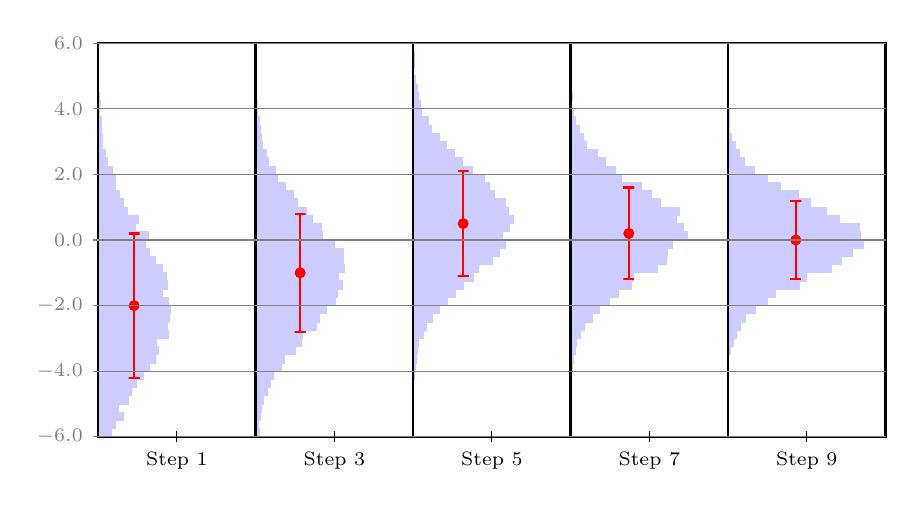
\begin{tikzpicture}
\begin{scope}[]
\pgfpathmoveto{ \pgfpointadd{\pgfpointxy {0.0} {0.0}} {\pgfpoint{0cm}{0.0cm}} }
\pgfpathlineto{ \pgfpointadd{\pgfpointxy {0.0} {0.0}} {\pgfpoint{2.0cm}{0.0cm}} }
\pgfpathlineto{ \pgfpointadd{\pgfpointxy {0.0} {0.0}} {\pgfpoint{2.0cm}{5.0cm}} }
\pgfpathlineto{ \pgfpointadd{\pgfpointxy {0.0} {0.0}} {\pgfpoint{0cm}{5.0cm}} }
\pgfpathclose
\pgfusepath{  clip, }
\begin{scope}[shift={(0.0,0.0)}]
\pgfsetxvec{\pgfpoint{0.002cm}{0cm}}
\pgfsetyvec{\pgfpoint{0cm}{0.41666666cm}}
\begin{scope}[shift={(-0.0,6.0)}]
\begin{scope}[fill=blue!20,draw=blue!20]
\pgfpathmoveto{ \pgfpointxy {0.0} {6.0}}
\pgfpathlineto{ \pgfpointxy {0.0} {6.0}}
\pgfpathlineto{ \pgfpointxy {0.0} {6.0}}
\pgfpathlineto{ \pgfpointxy {0.0} {5.75}}
\pgfpathlineto{ \pgfpointxy {2.0} {5.75}}
\pgfpathlineto{ \pgfpointxy {2.0} {5.5}}
\pgfpathlineto{ \pgfpointxy {4.0} {5.5}}
\pgfpathlineto{ \pgfpointxy {4.0} {5.25}}
\pgfpathlineto{ \pgfpointxy {0.0} {5.25}}
\pgfpathlineto{ \pgfpointxy {0.0} {5.0}}
\pgfpathlineto{ \pgfpointxy {3.0} {5.0}}
\pgfpathlineto{ \pgfpointxy {3.0} {4.75}}
\pgfpathlineto{ \pgfpointxy {3.0} {4.75}}
\pgfpathlineto{ \pgfpointxy {3.0} {4.5}}
\pgfpathlineto{ \pgfpointxy {8.0} {4.5}}
\pgfpathlineto{ \pgfpointxy {8.0} {4.25}}
\pgfpathlineto{ \pgfpointxy {15.0} {4.25}}
\pgfpathlineto{ \pgfpointxy {15.0} {4.0}}
\pgfpathlineto{ \pgfpointxy {11.0} {4.0}}
\pgfpathlineto{ \pgfpointxy {11.0} {3.75}}
\pgfpathlineto{ \pgfpointxy {20.0} {3.75}}
\pgfpathlineto{ \pgfpointxy {20.0} {3.5}}
\pgfpathlineto{ \pgfpointxy {22.0} {3.5}}
\pgfpathlineto{ \pgfpointxy {22.0} {3.25}}
\pgfpathlineto{ \pgfpointxy {25.0} {3.25}}
\pgfpathlineto{ \pgfpointxy {25.0} {3.0}}
\pgfpathlineto{ \pgfpointxy {30.0} {3.0}}
\pgfpathlineto{ \pgfpointxy {30.0} {2.75}}
\pgfpathlineto{ \pgfpointxy {46.0} {2.75}}
\pgfpathlineto{ \pgfpointxy {46.0} {2.5}}
\pgfpathlineto{ \pgfpointxy {56.0} {2.5}}
\pgfpathlineto{ \pgfpointxy {56.0} {2.25}}
\pgfpathlineto{ \pgfpointxy {90.0} {2.25}}
\pgfpathlineto{ \pgfpointxy {90.0} {2.0}}
\pgfpathlineto{ \pgfpointxy {110.0} {2.0}}
\pgfpathlineto{ \pgfpointxy {110.0} {1.75}}
\pgfpathlineto{ \pgfpointxy {107.0} {1.75}}
\pgfpathlineto{ \pgfpointxy {107.0} {1.5}}
\pgfpathlineto{ \pgfpointxy {135.0} {1.5}}
\pgfpathlineto{ \pgfpointxy {135.0} {1.25}}
\pgfpathlineto{ \pgfpointxy {158.0} {1.25}}
\pgfpathlineto{ \pgfpointxy {158.0} {1.0}}
\pgfpathlineto{ \pgfpointxy {186.0} {1.0}}
\pgfpathlineto{ \pgfpointxy {186.0} {0.75}}
\pgfpathlineto{ \pgfpointxy {256.0} {0.75}}
\pgfpathlineto{ \pgfpointxy {256.0} {0.5}}
\pgfpathlineto{ \pgfpointxy {238.0} {0.5}}
\pgfpathlineto{ \pgfpointxy {238.0} {0.25}}
\pgfpathlineto{ \pgfpointxy {319.0} {0.25}}
\pgfpathlineto{ \pgfpointxy {319.0} {0.0}}
\pgfpathlineto{ \pgfpointxy {300.0} {0.0}}
\pgfpathlineto{ \pgfpointxy {300.0} {-0.25}}
\pgfpathlineto{ \pgfpointxy {328.0} {-0.25}}
\pgfpathlineto{ \pgfpointxy {328.0} {-0.5}}
\pgfpathlineto{ \pgfpointxy {364.0} {-0.5}}
\pgfpathlineto{ \pgfpointxy {364.0} {-0.75}}
\pgfpathlineto{ \pgfpointxy {411.0} {-0.75}}
\pgfpathlineto{ \pgfpointxy {411.0} {-1.0}}
\pgfpathlineto{ \pgfpointxy {431.0} {-1.0}}
\pgfpathlineto{ \pgfpointxy {431.0} {-1.25}}
\pgfpathlineto{ \pgfpointxy {442.0} {-1.25}}
\pgfpathlineto{ \pgfpointxy {442.0} {-1.5}}
\pgfpathlineto{ \pgfpointxy {407.0} {-1.5}}
\pgfpathlineto{ \pgfpointxy {407.0} {-1.75}}
\pgfpathlineto{ \pgfpointxy {444.0} {-1.75}}
\pgfpathlineto{ \pgfpointxy {444.0} {-2.0}}
\pgfpathlineto{ \pgfpointxy {457.0} {-2.0}}
\pgfpathlineto{ \pgfpointxy {457.0} {-2.25}}
\pgfpathlineto{ \pgfpointxy {455.0} {-2.25}}
\pgfpathlineto{ \pgfpointxy {455.0} {-2.5}}
\pgfpathlineto{ \pgfpointxy {439.0} {-2.5}}
\pgfpathlineto{ \pgfpointxy {439.0} {-2.75}}
\pgfpathlineto{ \pgfpointxy {448.0} {-2.75}}
\pgfpathlineto{ \pgfpointxy {448.0} {-3.0}}
\pgfpathlineto{ \pgfpointxy {373.0} {-3.0}}
\pgfpathlineto{ \pgfpointxy {373.0} {-3.25}}
\pgfpathlineto{ \pgfpointxy {385.0} {-3.25}}
\pgfpathlineto{ \pgfpointxy {385.0} {-3.5}}
\pgfpathlineto{ \pgfpointxy {362.0} {-3.5}}
\pgfpathlineto{ \pgfpointxy {362.0} {-3.75}}
\pgfpathlineto{ \pgfpointxy {325.0} {-3.75}}
\pgfpathlineto{ \pgfpointxy {325.0} {-4.0}}
\pgfpathlineto{ \pgfpointxy {289.0} {-4.0}}
\pgfpathlineto{ \pgfpointxy {289.0} {-4.25}}
\pgfpathlineto{ \pgfpointxy {243.0} {-4.25}}
\pgfpathlineto{ \pgfpointxy {243.0} {-4.5}}
\pgfpathlineto{ \pgfpointxy {209.0} {-4.5}}
\pgfpathlineto{ \pgfpointxy {209.0} {-4.75}}
\pgfpathlineto{ \pgfpointxy {191.0} {-4.75}}
\pgfpathlineto{ \pgfpointxy {191.0} {-5.0}}
\pgfpathlineto{ \pgfpointxy {132.0} {-5.0}}
\pgfpathlineto{ \pgfpointxy {132.0} {-5.25}}
\pgfpathlineto{ \pgfpointxy {158.0} {-5.25}}
\pgfpathlineto{ \pgfpointxy {158.0} {-5.5}}
\pgfpathlineto{ \pgfpointxy {113.0} {-5.5}}
\pgfpathlineto{ \pgfpointxy {113.0} {-5.75}}
\pgfpathlineto{ \pgfpointxy {86.0} {-5.75}}
\pgfpathlineto{ \pgfpointxy {86.0} {-6.0}}
\pgfpathlineto{ \pgfpointxy {0.0} {-6.0}}
\pgfusepath{ stroke, fill, }
\end{scope}
\end{scope}
\pgfsetxvec{\pgfpoint{1cm}{0cm}}
\pgfsetyvec{\pgfpoint{0cm}{1cm}}
\end{scope}
\end{scope}
\begin{scope}[shift={(0.0,0.0)}]
\pgfsetxvec{\pgfpoint{0.002cm}{0cm}}
\pgfsetyvec{\pgfpoint{0cm}{0.41666666cm}}
\begin{scope}[shift={(-0.0,6.0)}]
\begin{scope}[red,fill=red,thick]
\pgfpathmoveto{ \pgfpointadd{\pgfpointxy {228.5} {0.20000005}} {\pgfpoint{-2pt}{0}} }
\pgfpathlineto{ \pgfpointadd{\pgfpointxy {228.5} {0.20000005}} {\pgfpoint{2pt}{0}} }
\pgfpathlineto{ \pgfpointadd{\pgfpointxy {228.5} {0.20000005}} {\pgfpoint{0pt}{0}} }
\pgfpathlineto{ \pgfpointadd{\pgfpointxy {228.5} {-4.2}} {\pgfpoint{0pt}{0}} }
\pgfpathlineto{ \pgfpointadd{\pgfpointxy {228.5} {-4.2}} {\pgfpoint{-2pt}{0}} }
\pgfpathlineto{ \pgfpointadd{\pgfpointxy {228.5} {-4.2}} {\pgfpoint{2pt}{0}} }
\pgfusepath{ stroke, }
\node at (228.5,-2.0) [red,fill=red,thick,circle,inner sep=0.0pt,minimum width =4.0pt,minimum height=4.0pt] {};
\end{scope}
\end{scope}
\pgfsetxvec{\pgfpoint{1cm}{0cm}}
\pgfsetyvec{\pgfpoint{0cm}{1cm}}
\end{scope}
\begin{scope}[shift={(0.0,0.0)}]
\pgfsetxvec{\pgfpoint{0.002cm}{0cm}}
\pgfsetyvec{\pgfpoint{0cm}{0.41666666cm}}
\begin{scope}[shift={(-0.0,6.0)}]
\begin{scope}[thick,black,fill=white]
\pgfpathmoveto{ \pgfpointxy {0.0} {-6.0}}
\pgfpathlineto{ \pgfpointxy {1000.0} {-6.0}}
\pgfpathlineto{ \pgfpointxy {1000.0} {6.0}}
\pgfpathlineto{ \pgfpointxy {0.0} {6.0}}
\pgfpathclose
\pgfusepath{ stroke, }
\end{scope}
\begin{scope}[yshift=0cm]
\end{scope}
\begin{scope}[xshift=0cm]
\end{scope}
\end{scope}
\pgfsetxvec{\pgfpoint{1cm}{0cm}}
\pgfsetyvec{\pgfpoint{0cm}{1cm}}
\end{scope}
\begin{scope}[]
\pgfpathmoveto{ \pgfpointadd{\pgfpointxy {0.0} {0.0}} {\pgfpoint{2cm}{0.0cm}} }
\pgfpathlineto{ \pgfpointadd{\pgfpointxy {0.0} {0.0}} {\pgfpoint{4.0cm}{0.0cm}} }
\pgfpathlineto{ \pgfpointadd{\pgfpointxy {0.0} {0.0}} {\pgfpoint{4.0cm}{5.0cm}} }
\pgfpathlineto{ \pgfpointadd{\pgfpointxy {0.0} {0.0}} {\pgfpoint{2cm}{5.0cm}} }
\pgfpathclose
\pgfusepath{  clip, }
\begin{scope}[shift={(2.0,0.0)}]
\pgfsetxvec{\pgfpoint{0.002cm}{0cm}}
\pgfsetyvec{\pgfpoint{0cm}{0.41666666cm}}
\begin{scope}[shift={(-0.0,6.0)}]
\begin{scope}[fill=blue!20,draw=blue!20]
\pgfpathmoveto{ \pgfpointxy {0.0} {6.0}}
\pgfpathlineto{ \pgfpointxy {0.0} {6.0}}
\pgfpathlineto{ \pgfpointxy {0.0} {6.0}}
\pgfpathlineto{ \pgfpointxy {0.0} {5.75}}
\pgfpathlineto{ \pgfpointxy {1.0} {5.75}}
\pgfpathlineto{ \pgfpointxy {1.0} {5.5}}
\pgfpathlineto{ \pgfpointxy {0.0} {5.5}}
\pgfpathlineto{ \pgfpointxy {0.0} {5.25}}
\pgfpathlineto{ \pgfpointxy {2.0} {5.25}}
\pgfpathlineto{ \pgfpointxy {2.0} {5.0}}
\pgfpathlineto{ \pgfpointxy {3.0} {5.0}}
\pgfpathlineto{ \pgfpointxy {3.0} {4.75}}
\pgfpathlineto{ \pgfpointxy {5.0} {4.75}}
\pgfpathlineto{ \pgfpointxy {5.0} {4.5}}
\pgfpathlineto{ \pgfpointxy {5.0} {4.5}}
\pgfpathlineto{ \pgfpointxy {5.0} {4.25}}
\pgfpathlineto{ \pgfpointxy {12.0} {4.25}}
\pgfpathlineto{ \pgfpointxy {12.0} {4.0}}
\pgfpathlineto{ \pgfpointxy {10.0} {4.0}}
\pgfpathlineto{ \pgfpointxy {10.0} {3.75}}
\pgfpathlineto{ \pgfpointxy {24.0} {3.75}}
\pgfpathlineto{ \pgfpointxy {24.0} {3.5}}
\pgfpathlineto{ \pgfpointxy {29.0} {3.5}}
\pgfpathlineto{ \pgfpointxy {29.0} {3.25}}
\pgfpathlineto{ \pgfpointxy {37.0} {3.25}}
\pgfpathlineto{ \pgfpointxy {37.0} {3.0}}
\pgfpathlineto{ \pgfpointxy {43.0} {3.0}}
\pgfpathlineto{ \pgfpointxy {43.0} {2.75}}
\pgfpathlineto{ \pgfpointxy {71.0} {2.75}}
\pgfpathlineto{ \pgfpointxy {71.0} {2.5}}
\pgfpathlineto{ \pgfpointxy {83.0} {2.5}}
\pgfpathlineto{ \pgfpointxy {83.0} {2.25}}
\pgfpathlineto{ \pgfpointxy {124.0} {2.25}}
\pgfpathlineto{ \pgfpointxy {124.0} {2.0}}
\pgfpathlineto{ \pgfpointxy {141.0} {2.0}}
\pgfpathlineto{ \pgfpointxy {141.0} {1.75}}
\pgfpathlineto{ \pgfpointxy {192.0} {1.75}}
\pgfpathlineto{ \pgfpointxy {192.0} {1.5}}
\pgfpathlineto{ \pgfpointxy {238.0} {1.5}}
\pgfpathlineto{ \pgfpointxy {238.0} {1.25}}
\pgfpathlineto{ \pgfpointxy {267.0} {1.25}}
\pgfpathlineto{ \pgfpointxy {267.0} {1.0}}
\pgfpathlineto{ \pgfpointxy {324.0} {1.0}}
\pgfpathlineto{ \pgfpointxy {324.0} {0.75}}
\pgfpathlineto{ \pgfpointxy {359.0} {0.75}}
\pgfpathlineto{ \pgfpointxy {359.0} {0.5}}
\pgfpathlineto{ \pgfpointxy {419.0} {0.5}}
\pgfpathlineto{ \pgfpointxy {419.0} {0.25}}
\pgfpathlineto{ \pgfpointxy {424.0} {0.25}}
\pgfpathlineto{ \pgfpointxy {424.0} {0.0}}
\pgfpathlineto{ \pgfpointxy {498.0} {0.0}}
\pgfpathlineto{ \pgfpointxy {498.0} {-0.25}}
\pgfpathlineto{ \pgfpointxy {555.0} {-0.25}}
\pgfpathlineto{ \pgfpointxy {555.0} {-0.5}}
\pgfpathlineto{ \pgfpointxy {556.0} {-0.5}}
\pgfpathlineto{ \pgfpointxy {556.0} {-0.75}}
\pgfpathlineto{ \pgfpointxy {566.0} {-0.75}}
\pgfpathlineto{ \pgfpointxy {566.0} {-1.0}}
\pgfpathlineto{ \pgfpointxy {528.0} {-1.0}}
\pgfpathlineto{ \pgfpointxy {528.0} {-1.25}}
\pgfpathlineto{ \pgfpointxy {550.0} {-1.25}}
\pgfpathlineto{ \pgfpointxy {550.0} {-1.5}}
\pgfpathlineto{ \pgfpointxy {523.0} {-1.5}}
\pgfpathlineto{ \pgfpointxy {523.0} {-1.75}}
\pgfpathlineto{ \pgfpointxy {509.0} {-1.75}}
\pgfpathlineto{ \pgfpointxy {509.0} {-2.0}}
\pgfpathlineto{ \pgfpointxy {451.0} {-2.0}}
\pgfpathlineto{ \pgfpointxy {451.0} {-2.25}}
\pgfpathlineto{ \pgfpointxy {403.0} {-2.25}}
\pgfpathlineto{ \pgfpointxy {403.0} {-2.5}}
\pgfpathlineto{ \pgfpointxy {387.0} {-2.5}}
\pgfpathlineto{ \pgfpointxy {387.0} {-2.75}}
\pgfpathlineto{ \pgfpointxy {298.0} {-2.75}}
\pgfpathlineto{ \pgfpointxy {298.0} {-3.0}}
\pgfpathlineto{ \pgfpointxy {294.0} {-3.0}}
\pgfpathlineto{ \pgfpointxy {294.0} {-3.25}}
\pgfpathlineto{ \pgfpointxy {254.0} {-3.25}}
\pgfpathlineto{ \pgfpointxy {254.0} {-3.5}}
\pgfpathlineto{ \pgfpointxy {183.0} {-3.5}}
\pgfpathlineto{ \pgfpointxy {183.0} {-3.75}}
\pgfpathlineto{ \pgfpointxy {167.0} {-3.75}}
\pgfpathlineto{ \pgfpointxy {167.0} {-4.0}}
\pgfpathlineto{ \pgfpointxy {116.0} {-4.0}}
\pgfpathlineto{ \pgfpointxy {116.0} {-4.25}}
\pgfpathlineto{ \pgfpointxy {94.0} {-4.25}}
\pgfpathlineto{ \pgfpointxy {94.0} {-4.5}}
\pgfpathlineto{ \pgfpointxy {75.0} {-4.5}}
\pgfpathlineto{ \pgfpointxy {75.0} {-4.75}}
\pgfpathlineto{ \pgfpointxy {48.0} {-4.75}}
\pgfpathlineto{ \pgfpointxy {48.0} {-5.0}}
\pgfpathlineto{ \pgfpointxy {40.0} {-5.0}}
\pgfpathlineto{ \pgfpointxy {40.0} {-5.25}}
\pgfpathlineto{ \pgfpointxy {32.0} {-5.25}}
\pgfpathlineto{ \pgfpointxy {32.0} {-5.5}}
\pgfpathlineto{ \pgfpointxy {17.0} {-5.5}}
\pgfpathlineto{ \pgfpointxy {17.0} {-5.75}}
\pgfpathlineto{ \pgfpointxy {23.0} {-5.75}}
\pgfpathlineto{ \pgfpointxy {23.0} {-6.0}}
\pgfpathlineto{ \pgfpointxy {0.0} {-6.0}}
\pgfusepath{ stroke, fill, }
\end{scope}
\end{scope}
\pgfsetxvec{\pgfpoint{1cm}{0cm}}
\pgfsetyvec{\pgfpoint{0cm}{1cm}}
\end{scope}
\end{scope}
\begin{scope}[shift={(2.0,0.0)}]
\pgfsetxvec{\pgfpoint{0.002cm}{0cm}}
\pgfsetyvec{\pgfpoint{0cm}{0.41666666cm}}
\begin{scope}[shift={(-0.0,6.0)}]
\begin{scope}[red,fill=red,thick]
\pgfpathmoveto{ \pgfpointadd{\pgfpointxy {283.0} {0.79999995}} {\pgfpoint{-2pt}{0}} }
\pgfpathlineto{ \pgfpointadd{\pgfpointxy {283.0} {0.79999995}} {\pgfpoint{2pt}{0}} }
\pgfpathlineto{ \pgfpointadd{\pgfpointxy {283.0} {0.79999995}} {\pgfpoint{0pt}{0}} }
\pgfpathlineto{ \pgfpointadd{\pgfpointxy {283.0} {-2.8}} {\pgfpoint{0pt}{0}} }
\pgfpathlineto{ \pgfpointadd{\pgfpointxy {283.0} {-2.8}} {\pgfpoint{-2pt}{0}} }
\pgfpathlineto{ \pgfpointadd{\pgfpointxy {283.0} {-2.8}} {\pgfpoint{2pt}{0}} }
\pgfusepath{ stroke, }
\node at (283.0,-1.0) [red,fill=red,thick,circle,inner sep=0.0pt,minimum width =4.0pt,minimum height=4.0pt] {};
\end{scope}
\end{scope}
\pgfsetxvec{\pgfpoint{1cm}{0cm}}
\pgfsetyvec{\pgfpoint{0cm}{1cm}}
\end{scope}
\begin{scope}[shift={(2.0,0.0)}]
\pgfsetxvec{\pgfpoint{0.002cm}{0cm}}
\pgfsetyvec{\pgfpoint{0cm}{0.41666666cm}}
\begin{scope}[shift={(-0.0,6.0)}]
\begin{scope}[thick,black,fill=white]
\pgfpathmoveto{ \pgfpointxy {0.0} {-6.0}}
\pgfpathlineto{ \pgfpointxy {1000.0} {-6.0}}
\pgfpathlineto{ \pgfpointxy {1000.0} {6.0}}
\pgfpathlineto{ \pgfpointxy {0.0} {6.0}}
\pgfpathclose
\pgfusepath{ stroke, }
\end{scope}
\begin{scope}[yshift=0cm]
\end{scope}
\begin{scope}[xshift=0cm]
\end{scope}
\end{scope}
\pgfsetxvec{\pgfpoint{1cm}{0cm}}
\pgfsetyvec{\pgfpoint{0cm}{1cm}}
\end{scope}
\begin{scope}[]
\pgfpathmoveto{ \pgfpointadd{\pgfpointxy {0.0} {0.0}} {\pgfpoint{4cm}{0.0cm}} }
\pgfpathlineto{ \pgfpointadd{\pgfpointxy {0.0} {0.0}} {\pgfpoint{6.0cm}{0.0cm}} }
\pgfpathlineto{ \pgfpointadd{\pgfpointxy {0.0} {0.0}} {\pgfpoint{6.0cm}{5.0cm}} }
\pgfpathlineto{ \pgfpointadd{\pgfpointxy {0.0} {0.0}} {\pgfpoint{4cm}{5.0cm}} }
\pgfpathclose
\pgfusepath{  clip, }
\begin{scope}[shift={(4.0,0.0)}]
\pgfsetxvec{\pgfpoint{0.002cm}{0cm}}
\pgfsetyvec{\pgfpoint{0cm}{0.41666666cm}}
\begin{scope}[shift={(-0.0,6.0)}]
\begin{scope}[fill=blue!20,draw=blue!20]
\pgfpathmoveto{ \pgfpointxy {0.0} {6.0}}
\pgfpathlineto{ \pgfpointxy {2.0} {6.0}}
\pgfpathlineto{ \pgfpointxy {2.0} {6.0}}
\pgfpathlineto{ \pgfpointxy {2.0} {5.75}}
\pgfpathlineto{ \pgfpointxy {8.0} {5.75}}
\pgfpathlineto{ \pgfpointxy {8.0} {5.5}}
\pgfpathlineto{ \pgfpointxy {10.0} {5.5}}
\pgfpathlineto{ \pgfpointxy {10.0} {5.25}}
\pgfpathlineto{ \pgfpointxy {5.0} {5.25}}
\pgfpathlineto{ \pgfpointxy {5.0} {5.0}}
\pgfpathlineto{ \pgfpointxy {15.0} {5.0}}
\pgfpathlineto{ \pgfpointxy {15.0} {4.75}}
\pgfpathlineto{ \pgfpointxy {29.0} {4.75}}
\pgfpathlineto{ \pgfpointxy {29.0} {4.5}}
\pgfpathlineto{ \pgfpointxy {31.0} {4.5}}
\pgfpathlineto{ \pgfpointxy {31.0} {4.25}}
\pgfpathlineto{ \pgfpointxy {46.0} {4.25}}
\pgfpathlineto{ \pgfpointxy {46.0} {4.0}}
\pgfpathlineto{ \pgfpointxy {52.0} {4.0}}
\pgfpathlineto{ \pgfpointxy {52.0} {3.75}}
\pgfpathlineto{ \pgfpointxy {97.0} {3.75}}
\pgfpathlineto{ \pgfpointxy {97.0} {3.5}}
\pgfpathlineto{ \pgfpointxy {115.0} {3.5}}
\pgfpathlineto{ \pgfpointxy {115.0} {3.25}}
\pgfpathlineto{ \pgfpointxy {169.0} {3.25}}
\pgfpathlineto{ \pgfpointxy {169.0} {3.0}}
\pgfpathlineto{ \pgfpointxy {209.0} {3.0}}
\pgfpathlineto{ \pgfpointxy {209.0} {2.75}}
\pgfpathlineto{ \pgfpointxy {261.0} {2.75}}
\pgfpathlineto{ \pgfpointxy {261.0} {2.5}}
\pgfpathlineto{ \pgfpointxy {312.0} {2.5}}
\pgfpathlineto{ \pgfpointxy {312.0} {2.25}}
\pgfpathlineto{ \pgfpointxy {375.0} {2.25}}
\pgfpathlineto{ \pgfpointxy {375.0} {2.0}}
\pgfpathlineto{ \pgfpointxy {451.0} {2.0}}
\pgfpathlineto{ \pgfpointxy {451.0} {1.75}}
\pgfpathlineto{ \pgfpointxy {484.0} {1.75}}
\pgfpathlineto{ \pgfpointxy {484.0} {1.5}}
\pgfpathlineto{ \pgfpointxy {516.0} {1.5}}
\pgfpathlineto{ \pgfpointxy {516.0} {1.25}}
\pgfpathlineto{ \pgfpointxy {586.0} {1.25}}
\pgfpathlineto{ \pgfpointxy {586.0} {1.0}}
\pgfpathlineto{ \pgfpointxy {603.0} {1.0}}
\pgfpathlineto{ \pgfpointxy {603.0} {0.75}}
\pgfpathlineto{ \pgfpointxy {636.0} {0.75}}
\pgfpathlineto{ \pgfpointxy {636.0} {0.5}}
\pgfpathlineto{ \pgfpointxy {609.0} {0.5}}
\pgfpathlineto{ \pgfpointxy {609.0} {0.25}}
\pgfpathlineto{ \pgfpointxy {570.0} {0.25}}
\pgfpathlineto{ \pgfpointxy {570.0} {0.0}}
\pgfpathlineto{ \pgfpointxy {588.0} {0.0}}
\pgfpathlineto{ \pgfpointxy {588.0} {-0.25}}
\pgfpathlineto{ \pgfpointxy {548.0} {-0.25}}
\pgfpathlineto{ \pgfpointxy {548.0} {-0.5}}
\pgfpathlineto{ \pgfpointxy {506.0} {-0.5}}
\pgfpathlineto{ \pgfpointxy {506.0} {-0.75}}
\pgfpathlineto{ \pgfpointxy {412.0} {-0.75}}
\pgfpathlineto{ \pgfpointxy {412.0} {-1.0}}
\pgfpathlineto{ \pgfpointxy {384.0} {-1.0}}
\pgfpathlineto{ \pgfpointxy {384.0} {-1.25}}
\pgfpathlineto{ \pgfpointxy {318.0} {-1.25}}
\pgfpathlineto{ \pgfpointxy {318.0} {-1.5}}
\pgfpathlineto{ \pgfpointxy {272.0} {-1.5}}
\pgfpathlineto{ \pgfpointxy {272.0} {-1.75}}
\pgfpathlineto{ \pgfpointxy {216.0} {-1.75}}
\pgfpathlineto{ \pgfpointxy {216.0} {-2.0}}
\pgfpathlineto{ \pgfpointxy {167.0} {-2.0}}
\pgfpathlineto{ \pgfpointxy {167.0} {-2.25}}
\pgfpathlineto{ \pgfpointxy {124.0} {-2.25}}
\pgfpathlineto{ \pgfpointxy {124.0} {-2.5}}
\pgfpathlineto{ \pgfpointxy {83.0} {-2.5}}
\pgfpathlineto{ \pgfpointxy {83.0} {-2.75}}
\pgfpathlineto{ \pgfpointxy {68.0} {-2.75}}
\pgfpathlineto{ \pgfpointxy {68.0} {-3.0}}
\pgfpathlineto{ \pgfpointxy {35.0} {-3.0}}
\pgfpathlineto{ \pgfpointxy {35.0} {-3.25}}
\pgfpathlineto{ \pgfpointxy {27.0} {-3.25}}
\pgfpathlineto{ \pgfpointxy {27.0} {-3.5}}
\pgfpathlineto{ \pgfpointxy {23.0} {-3.5}}
\pgfpathlineto{ \pgfpointxy {23.0} {-3.75}}
\pgfpathlineto{ \pgfpointxy {15.0} {-3.75}}
\pgfpathlineto{ \pgfpointxy {15.0} {-4.0}}
\pgfpathlineto{ \pgfpointxy {10.0} {-4.0}}
\pgfpathlineto{ \pgfpointxy {10.0} {-4.25}}
\pgfpathlineto{ \pgfpointxy {2.0} {-4.25}}
\pgfpathlineto{ \pgfpointxy {2.0} {-4.5}}
\pgfpathlineto{ \pgfpointxy {3.0} {-4.5}}
\pgfpathlineto{ \pgfpointxy {3.0} {-4.75}}
\pgfpathlineto{ \pgfpointxy {2.0} {-4.75}}
\pgfpathlineto{ \pgfpointxy {2.0} {-5.0}}
\pgfpathlineto{ \pgfpointxy {3.0} {-5.0}}
\pgfpathlineto{ \pgfpointxy {3.0} {-5.25}}
\pgfpathlineto{ \pgfpointxy {0.0} {-5.25}}
\pgfpathlineto{ \pgfpointxy {0.0} {-5.5}}
\pgfpathlineto{ \pgfpointxy {0.0} {-5.5}}
\pgfpathlineto{ \pgfpointxy {0.0} {-5.75}}
\pgfpathlineto{ \pgfpointxy {0.0} {-5.75}}
\pgfpathlineto{ \pgfpointxy {0.0} {-6.0}}
\pgfpathlineto{ \pgfpointxy {0.0} {-6.0}}
\pgfusepath{ stroke, fill, }
\end{scope}
\end{scope}
\pgfsetxvec{\pgfpoint{1cm}{0cm}}
\pgfsetyvec{\pgfpoint{0cm}{1cm}}
\end{scope}
\end{scope}
\begin{scope}[shift={(4.0,0.0)}]
\pgfsetxvec{\pgfpoint{0.002cm}{0cm}}
\pgfsetyvec{\pgfpoint{0cm}{0.41666666cm}}
\begin{scope}[shift={(-0.0,6.0)}]
\begin{scope}[red,fill=red,thick]
\pgfpathmoveto{ \pgfpointadd{\pgfpointxy {318.0} {2.1}} {\pgfpoint{-2pt}{0}} }
\pgfpathlineto{ \pgfpointadd{\pgfpointxy {318.0} {2.1}} {\pgfpoint{2pt}{0}} }
\pgfpathlineto{ \pgfpointadd{\pgfpointxy {318.0} {2.1}} {\pgfpoint{0pt}{0}} }
\pgfpathlineto{ \pgfpointadd{\pgfpointxy {318.0} {-1.1}} {\pgfpoint{0pt}{0}} }
\pgfpathlineto{ \pgfpointadd{\pgfpointxy {318.0} {-1.1}} {\pgfpoint{-2pt}{0}} }
\pgfpathlineto{ \pgfpointadd{\pgfpointxy {318.0} {-1.1}} {\pgfpoint{2pt}{0}} }
\pgfusepath{ stroke, }
\node at (318.0,0.5) [red,fill=red,thick,circle,inner sep=0.0pt,minimum width =4.0pt,minimum height=4.0pt] {};
\end{scope}
\end{scope}
\pgfsetxvec{\pgfpoint{1cm}{0cm}}
\pgfsetyvec{\pgfpoint{0cm}{1cm}}
\end{scope}
\begin{scope}[shift={(4.0,0.0)}]
\pgfsetxvec{\pgfpoint{0.002cm}{0cm}}
\pgfsetyvec{\pgfpoint{0cm}{0.41666666cm}}
\begin{scope}[shift={(-0.0,6.0)}]
\begin{scope}[thick,black,fill=white]
\pgfpathmoveto{ \pgfpointxy {0.0} {-6.0}}
\pgfpathlineto{ \pgfpointxy {1000.0} {-6.0}}
\pgfpathlineto{ \pgfpointxy {1000.0} {6.0}}
\pgfpathlineto{ \pgfpointxy {0.0} {6.0}}
\pgfpathclose
\pgfusepath{ stroke, }
\end{scope}
\begin{scope}[yshift=0cm]
\end{scope}
\begin{scope}[xshift=0cm]
\end{scope}
\end{scope}
\pgfsetxvec{\pgfpoint{1cm}{0cm}}
\pgfsetyvec{\pgfpoint{0cm}{1cm}}
\end{scope}
\begin{scope}[]
\pgfpathmoveto{ \pgfpointadd{\pgfpointxy {0.0} {0.0}} {\pgfpoint{6cm}{0.0cm}} }
\pgfpathlineto{ \pgfpointadd{\pgfpointxy {0.0} {0.0}} {\pgfpoint{8.0cm}{0.0cm}} }
\pgfpathlineto{ \pgfpointadd{\pgfpointxy {0.0} {0.0}} {\pgfpoint{8.0cm}{5.0cm}} }
\pgfpathlineto{ \pgfpointadd{\pgfpointxy {0.0} {0.0}} {\pgfpoint{6cm}{5.0cm}} }
\pgfpathclose
\pgfusepath{  clip, }
\begin{scope}[shift={(6.0,0.0)}]
\pgfsetxvec{\pgfpoint{0.002cm}{0cm}}
\pgfsetyvec{\pgfpoint{0cm}{0.41666666cm}}
\begin{scope}[shift={(-0.0,6.0)}]
\begin{scope}[fill=blue!20,draw=blue!20]
\pgfpathmoveto{ \pgfpointxy {0.0} {6.0}}
\pgfpathlineto{ \pgfpointxy {0.0} {6.0}}
\pgfpathlineto{ \pgfpointxy {0.0} {6.0}}
\pgfpathlineto{ \pgfpointxy {0.0} {5.75}}
\pgfpathlineto{ \pgfpointxy {0.0} {5.75}}
\pgfpathlineto{ \pgfpointxy {0.0} {5.5}}
\pgfpathlineto{ \pgfpointxy {0.0} {5.5}}
\pgfpathlineto{ \pgfpointxy {0.0} {5.25}}
\pgfpathlineto{ \pgfpointxy {1.0} {5.25}}
\pgfpathlineto{ \pgfpointxy {1.0} {5.0}}
\pgfpathlineto{ \pgfpointxy {3.0} {5.0}}
\pgfpathlineto{ \pgfpointxy {3.0} {4.75}}
\pgfpathlineto{ \pgfpointxy {8.0} {4.75}}
\pgfpathlineto{ \pgfpointxy {8.0} {4.5}}
\pgfpathlineto{ \pgfpointxy {9.0} {4.5}}
\pgfpathlineto{ \pgfpointxy {9.0} {4.25}}
\pgfpathlineto{ \pgfpointxy {8.0} {4.25}}
\pgfpathlineto{ \pgfpointxy {8.0} {4.0}}
\pgfpathlineto{ \pgfpointxy {19.0} {4.0}}
\pgfpathlineto{ \pgfpointxy {19.0} {3.75}}
\pgfpathlineto{ \pgfpointxy {31.0} {3.75}}
\pgfpathlineto{ \pgfpointxy {31.0} {3.5}}
\pgfpathlineto{ \pgfpointxy {55.0} {3.5}}
\pgfpathlineto{ \pgfpointxy {55.0} {3.25}}
\pgfpathlineto{ \pgfpointxy {82.0} {3.25}}
\pgfpathlineto{ \pgfpointxy {82.0} {3.0}}
\pgfpathlineto{ \pgfpointxy {100.0} {3.0}}
\pgfpathlineto{ \pgfpointxy {100.0} {2.75}}
\pgfpathlineto{ \pgfpointxy {172.0} {2.75}}
\pgfpathlineto{ \pgfpointxy {172.0} {2.5}}
\pgfpathlineto{ \pgfpointxy {220.0} {2.5}}
\pgfpathlineto{ \pgfpointxy {220.0} {2.25}}
\pgfpathlineto{ \pgfpointxy {287.0} {2.25}}
\pgfpathlineto{ \pgfpointxy {287.0} {2.0}}
\pgfpathlineto{ \pgfpointxy {321.0} {2.0}}
\pgfpathlineto{ \pgfpointxy {321.0} {1.75}}
\pgfpathlineto{ \pgfpointxy {448.0} {1.75}}
\pgfpathlineto{ \pgfpointxy {448.0} {1.5}}
\pgfpathlineto{ \pgfpointxy {512.0} {1.5}}
\pgfpathlineto{ \pgfpointxy {512.0} {1.25}}
\pgfpathlineto{ \pgfpointxy {571.0} {1.25}}
\pgfpathlineto{ \pgfpointxy {571.0} {1.0}}
\pgfpathlineto{ \pgfpointxy {690.0} {1.0}}
\pgfpathlineto{ \pgfpointxy {690.0} {0.75}}
\pgfpathlineto{ \pgfpointxy {671.0} {0.75}}
\pgfpathlineto{ \pgfpointxy {671.0} {0.5}}
\pgfpathlineto{ \pgfpointxy {715.0} {0.5}}
\pgfpathlineto{ \pgfpointxy {715.0} {0.25}}
\pgfpathlineto{ \pgfpointxy {740.0} {0.25}}
\pgfpathlineto{ \pgfpointxy {740.0} {0.0}}
\pgfpathlineto{ \pgfpointxy {650.0} {0.0}}
\pgfpathlineto{ \pgfpointxy {650.0} {-0.25}}
\pgfpathlineto{ \pgfpointxy {617.0} {-0.25}}
\pgfpathlineto{ \pgfpointxy {617.0} {-0.5}}
\pgfpathlineto{ \pgfpointxy {609.0} {-0.5}}
\pgfpathlineto{ \pgfpointxy {609.0} {-0.75}}
\pgfpathlineto{ \pgfpointxy {550.0} {-0.75}}
\pgfpathlineto{ \pgfpointxy {550.0} {-1.0}}
\pgfpathlineto{ \pgfpointxy {401.0} {-1.0}}
\pgfpathlineto{ \pgfpointxy {401.0} {-1.25}}
\pgfpathlineto{ \pgfpointxy {386.0} {-1.25}}
\pgfpathlineto{ \pgfpointxy {386.0} {-1.5}}
\pgfpathlineto{ \pgfpointxy {301.0} {-1.5}}
\pgfpathlineto{ \pgfpointxy {301.0} {-1.75}}
\pgfpathlineto{ \pgfpointxy {247.0} {-1.75}}
\pgfpathlineto{ \pgfpointxy {247.0} {-2.0}}
\pgfpathlineto{ \pgfpointxy {181.0} {-2.0}}
\pgfpathlineto{ \pgfpointxy {181.0} {-2.25}}
\pgfpathlineto{ \pgfpointxy {140.0} {-2.25}}
\pgfpathlineto{ \pgfpointxy {140.0} {-2.5}}
\pgfpathlineto{ \pgfpointxy {88.0} {-2.5}}
\pgfpathlineto{ \pgfpointxy {88.0} {-2.75}}
\pgfpathlineto{ \pgfpointxy {61.0} {-2.75}}
\pgfpathlineto{ \pgfpointxy {61.0} {-3.0}}
\pgfpathlineto{ \pgfpointxy {37.0} {-3.0}}
\pgfpathlineto{ \pgfpointxy {37.0} {-3.25}}
\pgfpathlineto{ \pgfpointxy {29.0} {-3.25}}
\pgfpathlineto{ \pgfpointxy {29.0} {-3.5}}
\pgfpathlineto{ \pgfpointxy {21.0} {-3.5}}
\pgfpathlineto{ \pgfpointxy {21.0} {-3.75}}
\pgfpathlineto{ \pgfpointxy {9.0} {-3.75}}
\pgfpathlineto{ \pgfpointxy {9.0} {-4.0}}
\pgfpathlineto{ \pgfpointxy {7.0} {-4.0}}
\pgfpathlineto{ \pgfpointxy {7.0} {-4.25}}
\pgfpathlineto{ \pgfpointxy {2.0} {-4.25}}
\pgfpathlineto{ \pgfpointxy {2.0} {-4.5}}
\pgfpathlineto{ \pgfpointxy {1.0} {-4.5}}
\pgfpathlineto{ \pgfpointxy {1.0} {-4.75}}
\pgfpathlineto{ \pgfpointxy {0.0} {-4.75}}
\pgfpathlineto{ \pgfpointxy {0.0} {-5.0}}
\pgfpathlineto{ \pgfpointxy {0.0} {-5.0}}
\pgfpathlineto{ \pgfpointxy {0.0} {-5.25}}
\pgfpathlineto{ \pgfpointxy {0.0} {-5.25}}
\pgfpathlineto{ \pgfpointxy {0.0} {-5.5}}
\pgfpathlineto{ \pgfpointxy {0.0} {-5.5}}
\pgfpathlineto{ \pgfpointxy {0.0} {-5.75}}
\pgfpathlineto{ \pgfpointxy {0.0} {-5.75}}
\pgfpathlineto{ \pgfpointxy {0.0} {-6.0}}
\pgfpathlineto{ \pgfpointxy {0.0} {-6.0}}
\pgfusepath{ stroke, fill, }
\end{scope}
\end{scope}
\pgfsetxvec{\pgfpoint{1cm}{0cm}}
\pgfsetyvec{\pgfpoint{0cm}{1cm}}
\end{scope}
\end{scope}
\begin{scope}[shift={(6.0,0.0)}]
\pgfsetxvec{\pgfpoint{0.002cm}{0cm}}
\pgfsetyvec{\pgfpoint{0cm}{0.41666666cm}}
\begin{scope}[shift={(-0.0,6.0)}]
\begin{scope}[red,fill=red,thick]
\pgfpathmoveto{ \pgfpointadd{\pgfpointxy {370.0} {1.6}} {\pgfpoint{-2pt}{0}} }
\pgfpathlineto{ \pgfpointadd{\pgfpointxy {370.0} {1.6}} {\pgfpoint{2pt}{0}} }
\pgfpathlineto{ \pgfpointadd{\pgfpointxy {370.0} {1.6}} {\pgfpoint{0pt}{0}} }
\pgfpathlineto{ \pgfpointadd{\pgfpointxy {370.0} {-1.1999999}} {\pgfpoint{0pt}{0}} }
\pgfpathlineto{ \pgfpointadd{\pgfpointxy {370.0} {-1.1999999}} {\pgfpoint{-2pt}{0}} }
\pgfpathlineto{ \pgfpointadd{\pgfpointxy {370.0} {-1.1999999}} {\pgfpoint{2pt}{0}} }
\pgfusepath{ stroke, }
\node at (370.0,0.2) [red,fill=red,thick,circle,inner sep=0.0pt,minimum width =4.0pt,minimum height=4.0pt] {};
\end{scope}
\end{scope}
\pgfsetxvec{\pgfpoint{1cm}{0cm}}
\pgfsetyvec{\pgfpoint{0cm}{1cm}}
\end{scope}
\begin{scope}[shift={(6.0,0.0)}]
\pgfsetxvec{\pgfpoint{0.002cm}{0cm}}
\pgfsetyvec{\pgfpoint{0cm}{0.41666666cm}}
\begin{scope}[shift={(-0.0,6.0)}]
\begin{scope}[thick,black,fill=white]
\pgfpathmoveto{ \pgfpointxy {0.0} {-6.0}}
\pgfpathlineto{ \pgfpointxy {1000.0} {-6.0}}
\pgfpathlineto{ \pgfpointxy {1000.0} {6.0}}
\pgfpathlineto{ \pgfpointxy {0.0} {6.0}}
\pgfpathclose
\pgfusepath{ stroke, }
\end{scope}
\begin{scope}[yshift=0cm]
\end{scope}
\begin{scope}[xshift=0cm]
\end{scope}
\end{scope}
\pgfsetxvec{\pgfpoint{1cm}{0cm}}
\pgfsetyvec{\pgfpoint{0cm}{1cm}}
\end{scope}
\begin{scope}[]
\pgfpathmoveto{ \pgfpointadd{\pgfpointxy {0.0} {0.0}} {\pgfpoint{8cm}{0.0cm}} }
\pgfpathlineto{ \pgfpointadd{\pgfpointxy {0.0} {0.0}} {\pgfpoint{10.0cm}{0.0cm}} }
\pgfpathlineto{ \pgfpointadd{\pgfpointxy {0.0} {0.0}} {\pgfpoint{10.0cm}{5.0cm}} }
\pgfpathlineto{ \pgfpointadd{\pgfpointxy {0.0} {0.0}} {\pgfpoint{8cm}{5.0cm}} }
\pgfpathclose
\pgfusepath{  clip, }
\begin{scope}[shift={(8.0,0.0)}]
\pgfsetxvec{\pgfpoint{0.002cm}{0cm}}
\pgfsetyvec{\pgfpoint{0cm}{0.41666666cm}}
\begin{scope}[shift={(-0.0,6.0)}]
\begin{scope}[fill=blue!20,draw=blue!20]
\pgfpathmoveto{ \pgfpointxy {0.0} {6.0}}
\pgfpathlineto{ \pgfpointxy {0.0} {6.0}}
\pgfpathlineto{ \pgfpointxy {0.0} {6.0}}
\pgfpathlineto{ \pgfpointxy {0.0} {5.75}}
\pgfpathlineto{ \pgfpointxy {0.0} {5.75}}
\pgfpathlineto{ \pgfpointxy {0.0} {5.5}}
\pgfpathlineto{ \pgfpointxy {0.0} {5.5}}
\pgfpathlineto{ \pgfpointxy {0.0} {5.25}}
\pgfpathlineto{ \pgfpointxy {0.0} {5.25}}
\pgfpathlineto{ \pgfpointxy {0.0} {5.0}}
\pgfpathlineto{ \pgfpointxy {0.0} {5.0}}
\pgfpathlineto{ \pgfpointxy {0.0} {4.75}}
\pgfpathlineto{ \pgfpointxy {0.0} {4.75}}
\pgfpathlineto{ \pgfpointxy {0.0} {4.5}}
\pgfpathlineto{ \pgfpointxy {0.0} {4.5}}
\pgfpathlineto{ \pgfpointxy {0.0} {4.25}}
\pgfpathlineto{ \pgfpointxy {2.0} {4.25}}
\pgfpathlineto{ \pgfpointxy {2.0} {4.0}}
\pgfpathlineto{ \pgfpointxy {9.0} {4.0}}
\pgfpathlineto{ \pgfpointxy {9.0} {3.75}}
\pgfpathlineto{ \pgfpointxy {8.0} {3.75}}
\pgfpathlineto{ \pgfpointxy {8.0} {3.5}}
\pgfpathlineto{ \pgfpointxy {11.0} {3.5}}
\pgfpathlineto{ \pgfpointxy {11.0} {3.25}}
\pgfpathlineto{ \pgfpointxy {22.0} {3.25}}
\pgfpathlineto{ \pgfpointxy {22.0} {3.0}}
\pgfpathlineto{ \pgfpointxy {48.0} {3.0}}
\pgfpathlineto{ \pgfpointxy {48.0} {2.75}}
\pgfpathlineto{ \pgfpointxy {73.0} {2.75}}
\pgfpathlineto{ \pgfpointxy {73.0} {2.5}}
\pgfpathlineto{ \pgfpointxy {102.0} {2.5}}
\pgfpathlineto{ \pgfpointxy {102.0} {2.25}}
\pgfpathlineto{ \pgfpointxy {165.0} {2.25}}
\pgfpathlineto{ \pgfpointxy {165.0} {2.0}}
\pgfpathlineto{ \pgfpointxy {248.0} {2.0}}
\pgfpathlineto{ \pgfpointxy {248.0} {1.75}}
\pgfpathlineto{ \pgfpointxy {333.0} {1.75}}
\pgfpathlineto{ \pgfpointxy {333.0} {1.5}}
\pgfpathlineto{ \pgfpointxy {448.0} {1.5}}
\pgfpathlineto{ \pgfpointxy {448.0} {1.25}}
\pgfpathlineto{ \pgfpointxy {524.0} {1.25}}
\pgfpathlineto{ \pgfpointxy {524.0} {1.0}}
\pgfpathlineto{ \pgfpointxy {625.0} {1.0}}
\pgfpathlineto{ \pgfpointxy {625.0} {0.75}}
\pgfpathlineto{ \pgfpointxy {705.0} {0.75}}
\pgfpathlineto{ \pgfpointxy {705.0} {0.5}}
\pgfpathlineto{ \pgfpointxy {832.0} {0.5}}
\pgfpathlineto{ \pgfpointxy {832.0} {0.25}}
\pgfpathlineto{ \pgfpointxy {839.0} {0.25}}
\pgfpathlineto{ \pgfpointxy {839.0} {0.0}}
\pgfpathlineto{ \pgfpointxy {860.0} {0.0}}
\pgfpathlineto{ \pgfpointxy {860.0} {-0.25}}
\pgfpathlineto{ \pgfpointxy {788.0} {-0.25}}
\pgfpathlineto{ \pgfpointxy {788.0} {-0.5}}
\pgfpathlineto{ \pgfpointxy {721.0} {-0.5}}
\pgfpathlineto{ \pgfpointxy {721.0} {-0.75}}
\pgfpathlineto{ \pgfpointxy {655.0} {-0.75}}
\pgfpathlineto{ \pgfpointxy {655.0} {-1.0}}
\pgfpathlineto{ \pgfpointxy {497.0} {-1.0}}
\pgfpathlineto{ \pgfpointxy {497.0} {-1.25}}
\pgfpathlineto{ \pgfpointxy {452.0} {-1.25}}
\pgfpathlineto{ \pgfpointxy {452.0} {-1.5}}
\pgfpathlineto{ \pgfpointxy {303.0} {-1.5}}
\pgfpathlineto{ \pgfpointxy {303.0} {-1.75}}
\pgfpathlineto{ \pgfpointxy {250.0} {-1.75}}
\pgfpathlineto{ \pgfpointxy {250.0} {-2.0}}
\pgfpathlineto{ \pgfpointxy {173.0} {-2.0}}
\pgfpathlineto{ \pgfpointxy {173.0} {-2.25}}
\pgfpathlineto{ \pgfpointxy {112.0} {-2.25}}
\pgfpathlineto{ \pgfpointxy {112.0} {-2.5}}
\pgfpathlineto{ \pgfpointxy {79.0} {-2.5}}
\pgfpathlineto{ \pgfpointxy {79.0} {-2.75}}
\pgfpathlineto{ \pgfpointxy {53.0} {-2.75}}
\pgfpathlineto{ \pgfpointxy {53.0} {-3.0}}
\pgfpathlineto{ \pgfpointxy {34.0} {-3.0}}
\pgfpathlineto{ \pgfpointxy {34.0} {-3.25}}
\pgfpathlineto{ \pgfpointxy {15.0} {-3.25}}
\pgfpathlineto{ \pgfpointxy {15.0} {-3.5}}
\pgfpathlineto{ \pgfpointxy {5.0} {-3.5}}
\pgfpathlineto{ \pgfpointxy {5.0} {-3.75}}
\pgfpathlineto{ \pgfpointxy {5.0} {-3.75}}
\pgfpathlineto{ \pgfpointxy {5.0} {-4.0}}
\pgfpathlineto{ \pgfpointxy {3.0} {-4.0}}
\pgfpathlineto{ \pgfpointxy {3.0} {-4.25}}
\pgfpathlineto{ \pgfpointxy {1.0} {-4.25}}
\pgfpathlineto{ \pgfpointxy {1.0} {-4.5}}
\pgfpathlineto{ \pgfpointxy {0.0} {-4.5}}
\pgfpathlineto{ \pgfpointxy {0.0} {-4.75}}
\pgfpathlineto{ \pgfpointxy {0.0} {-4.75}}
\pgfpathlineto{ \pgfpointxy {0.0} {-5.0}}
\pgfpathlineto{ \pgfpointxy {0.0} {-5.0}}
\pgfpathlineto{ \pgfpointxy {0.0} {-5.25}}
\pgfpathlineto{ \pgfpointxy {0.0} {-5.25}}
\pgfpathlineto{ \pgfpointxy {0.0} {-5.5}}
\pgfpathlineto{ \pgfpointxy {0.0} {-5.5}}
\pgfpathlineto{ \pgfpointxy {0.0} {-5.75}}
\pgfpathlineto{ \pgfpointxy {0.0} {-5.75}}
\pgfpathlineto{ \pgfpointxy {0.0} {-6.0}}
\pgfpathlineto{ \pgfpointxy {0.0} {-6.0}}
\pgfusepath{ stroke, fill, }
\end{scope}
\end{scope}
\pgfsetxvec{\pgfpoint{1cm}{0cm}}
\pgfsetyvec{\pgfpoint{0cm}{1cm}}
\end{scope}
\end{scope}
\begin{scope}[shift={(8.0,0.0)}]
\pgfsetxvec{\pgfpoint{0.002cm}{0cm}}
\pgfsetyvec{\pgfpoint{0cm}{0.41666666cm}}
\begin{scope}[shift={(-0.0,6.0)}]
\begin{scope}[red,fill=red,thick]
\pgfpathmoveto{ \pgfpointadd{\pgfpointxy {430.0} {1.2}} {\pgfpoint{-2pt}{0}} }
\pgfpathlineto{ \pgfpointadd{\pgfpointxy {430.0} {1.2}} {\pgfpoint{2pt}{0}} }
\pgfpathlineto{ \pgfpointadd{\pgfpointxy {430.0} {1.2}} {\pgfpoint{0pt}{0}} }
\pgfpathlineto{ \pgfpointadd{\pgfpointxy {430.0} {-1.2}} {\pgfpoint{0pt}{0}} }
\pgfpathlineto{ \pgfpointadd{\pgfpointxy {430.0} {-1.2}} {\pgfpoint{-2pt}{0}} }
\pgfpathlineto{ \pgfpointadd{\pgfpointxy {430.0} {-1.2}} {\pgfpoint{2pt}{0}} }
\pgfusepath{ stroke, }
\node at (430.0,0.0) [red,fill=red,thick,circle,inner sep=0.0pt,minimum width =4.0pt,minimum height=4.0pt] {};
\end{scope}
\end{scope}
\pgfsetxvec{\pgfpoint{1cm}{0cm}}
\pgfsetyvec{\pgfpoint{0cm}{1cm}}
\end{scope}
\begin{scope}[shift={(8.0,0.0)}]
\pgfsetxvec{\pgfpoint{0.002cm}{0cm}}
\pgfsetyvec{\pgfpoint{0cm}{0.41666666cm}}
\begin{scope}[shift={(-0.0,6.0)}]
\begin{scope}[thick,black,fill=white]
\pgfpathmoveto{ \pgfpointxy {0.0} {-6.0}}
\pgfpathlineto{ \pgfpointxy {1000.0} {-6.0}}
\pgfpathlineto{ \pgfpointxy {1000.0} {6.0}}
\pgfpathlineto{ \pgfpointxy {0.0} {6.0}}
\pgfpathclose
\pgfusepath{ stroke, }
\end{scope}
\begin{scope}[yshift=0cm]
\end{scope}
\begin{scope}[xshift=0cm]
\end{scope}
\end{scope}
\pgfsetxvec{\pgfpoint{1cm}{0cm}}
\pgfsetyvec{\pgfpoint{0cm}{1cm}}
\end{scope}
\begin{scope}[shift={(0.0,0.0)}]
\pgfsetxvec{\pgfpoint{1.0cm}{0cm}}
\pgfsetyvec{\pgfpoint{0cm}{0.41666666cm}}
\begin{scope}[shift={(-0.0,6.0)}]
\begin{scope}[xshift=0cm]
\draw[gray] [shift={(0.0,-6.0)}] (10cm,0) -- (-2pt,0) node[left]{ \scriptsize{\num[round-mode=places,round-precision=1]{-6.0}}};
\draw[gray] [shift={(0.0,-4.0)}] (10cm,0) -- (-2pt,0) node[left]{ \scriptsize{\num[round-mode=places,round-precision=1]{-4.0}}};
\draw[gray] [shift={(0.0,-2.0)}] (10cm,0) -- (-2pt,0) node[left]{ \scriptsize{\num[round-mode=places,round-precision=1]{-2.0}}};
\draw[gray] [shift={(0.0,0.0)}] (10cm,0) -- (-2pt,0) node[left]{ \scriptsize{\num[round-mode=places,round-precision=1]{0.0}}};
\draw[gray] [shift={(0.0,2.0)}] (10cm,0) -- (-2pt,0) node[left]{ \scriptsize{\num[round-mode=places,round-precision=1]{2.0}}};
\draw[gray] [shift={(0.0,4.0)}] (10cm,0) -- (-2pt,0) node[left]{ \scriptsize{\num[round-mode=places,round-precision=1]{4.0}}};
\draw[gray] [shift={(0.0,6.0)}] (10cm,0) -- (-2pt,0) node[left]{ \scriptsize{\num[round-mode=places,round-precision=1]{6.0}}};
\end{scope}
\end{scope}
\pgfsetxvec{\pgfpoint{1cm}{0cm}}
\pgfsetyvec{\pgfpoint{0cm}{1cm}}
\end{scope}
\begin{scope}[shift={(0.0,0.0)}]
\pgfsetxvec{\pgfpoint{1.0cm}{0cm}}
\pgfsetyvec{\pgfpoint{0cm}{0.41666666cm}}
\begin{scope}[shift={(-0.0,6.0)}]
\begin{scope}[yshift=0cm]
\draw[black] [shift={(1.0,-6.0)}] (0,2pt) -- (0,-2pt) node[below]{ \scriptsize{Step 1}};
\draw[black] [shift={(3.0,-6.0)}] (0,2pt) -- (0,-2pt) node[below]{ \scriptsize{Step 3}};
\draw[black] [shift={(5.0,-6.0)}] (0,2pt) -- (0,-2pt) node[below]{ \scriptsize{Step 5}};
\draw[black] [shift={(7.0,-6.0)}] (0,2pt) -- (0,-2pt) node[below]{ \scriptsize{Step 7}};
\draw[black] [shift={(9.0,-6.0)}] (0,2pt) -- (0,-2pt) node[below]{ \scriptsize{Step 9}};
\end{scope}
\end{scope}
\pgfsetxvec{\pgfpoint{1cm}{0cm}}
\pgfsetyvec{\pgfpoint{0cm}{1cm}}
\end{scope}
\end{tikzpicture}
\end{document}

  \caption{ Histograms with mean and sigmas.}
\end{figure}

\begin{figure}[H]
  \centering
  \documentclass{standalone}
\ifx\HCode\UnDef\else\def\pgfsysdriver{pgfsys-tex4ht.def}\fi
\usepackage{tikz}
\usepackage{color}
\usepackage{siunitx}
\usetikzlibrary{arrows,shapes}
\begin{document}
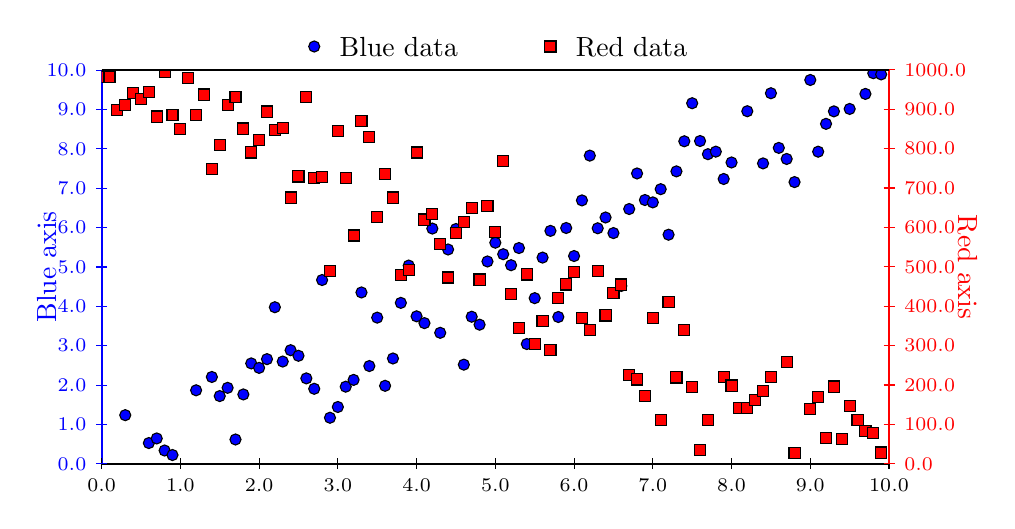
\begin{tikzpicture}
\draw[thick,black] (0.0,0.0) -- (10.0,0.0);
\draw[thick,blue] (0.0,0.0) -- (0.0,5.0);
\node[rotate=90,blue] at (-0.7,2.5) {Blue axis};
\begin{scope}[shift={(0.0,0.0)}]
\pgfsetxvec{\pgfpoint{1.0cm}{0cm}}
\pgfsetyvec{\pgfpoint{0cm}{0.5cm}}
\begin{scope}[shift={(0.0,0.0)}]
\begin{scope}[yshift=0cm]
\draw[black] [shift={(0.0,0.0)}] (0,2pt) -- (0,-2pt) node[below]{ \scriptsize{\num[round-mode=places,round-precision=1]{0}}};
\draw[black] [shift={(1.0,0.0)}] (0,2pt) -- (0,-2pt) node[below]{ \scriptsize{\num[round-mode=places,round-precision=1]{1}}};
\draw[black] [shift={(2.0,0.0)}] (0,2pt) -- (0,-2pt) node[below]{ \scriptsize{\num[round-mode=places,round-precision=1]{2}}};
\draw[black] [shift={(3.0,0.0)}] (0,2pt) -- (0,-2pt) node[below]{ \scriptsize{\num[round-mode=places,round-precision=1]{3}}};
\draw[black] [shift={(4.0,0.0)}] (0,2pt) -- (0,-2pt) node[below]{ \scriptsize{\num[round-mode=places,round-precision=1]{4}}};
\draw[black] [shift={(5.0,0.0)}] (0,2pt) -- (0,-2pt) node[below]{ \scriptsize{\num[round-mode=places,round-precision=1]{5}}};
\draw[black] [shift={(6.0,0.0)}] (0,2pt) -- (0,-2pt) node[below]{ \scriptsize{\num[round-mode=places,round-precision=1]{6}}};
\draw[black] [shift={(7.0,0.0)}] (0,2pt) -- (0,-2pt) node[below]{ \scriptsize{\num[round-mode=places,round-precision=1]{7}}};
\draw[black] [shift={(8.0,0.0)}] (0,2pt) -- (0,-2pt) node[below]{ \scriptsize{\num[round-mode=places,round-precision=1]{8}}};
\draw[black] [shift={(9.0,0.0)}] (0,2pt) -- (0,-2pt) node[below]{ \scriptsize{\num[round-mode=places,round-precision=1]{9}}};
\draw[black] [shift={(10.0,0.0)}] (0,2pt) -- (0,-2pt) node[below]{ \scriptsize{\num[round-mode=places,round-precision=1]{10}}};
\end{scope}
\begin{scope}[xshift=0cm]
\draw[blue] [shift={(0.0,0.0)}] (2pt,0) -- (-2pt,0) node[left]{ \scriptsize{\num[round-mode=places,round-precision=1]{0}}};
\draw[blue] [shift={(0.0,1.0)}] (2pt,0) -- (-2pt,0) node[left]{ \scriptsize{\num[round-mode=places,round-precision=1]{1}}};
\draw[blue] [shift={(0.0,2.0)}] (2pt,0) -- (-2pt,0) node[left]{ \scriptsize{\num[round-mode=places,round-precision=1]{2}}};
\draw[blue] [shift={(0.0,3.0)}] (2pt,0) -- (-2pt,0) node[left]{ \scriptsize{\num[round-mode=places,round-precision=1]{3}}};
\draw[blue] [shift={(0.0,4.0)}] (2pt,0) -- (-2pt,0) node[left]{ \scriptsize{\num[round-mode=places,round-precision=1]{4}}};
\draw[blue] [shift={(0.0,5.0)}] (2pt,0) -- (-2pt,0) node[left]{ \scriptsize{\num[round-mode=places,round-precision=1]{5}}};
\draw[blue] [shift={(0.0,6.0)}] (2pt,0) -- (-2pt,0) node[left]{ \scriptsize{\num[round-mode=places,round-precision=1]{6}}};
\draw[blue] [shift={(0.0,7.0)}] (2pt,0) -- (-2pt,0) node[left]{ \scriptsize{\num[round-mode=places,round-precision=1]{7}}};
\draw[blue] [shift={(0.0,8.0)}] (2pt,0) -- (-2pt,0) node[left]{ \scriptsize{\num[round-mode=places,round-precision=1]{8}}};
\draw[blue] [shift={(0.0,9.0)}] (2pt,0) -- (-2pt,0) node[left]{ \scriptsize{\num[round-mode=places,round-precision=1]{9}}};
\draw[blue] [shift={(0.0,10.0)}] (2pt,0) -- (-2pt,0) node[left]{ \scriptsize{\num[round-mode=places,round-precision=1]{10}}};
\end{scope}
\end{scope}
\pgfsetxvec{\pgfpoint{1cm}{0cm}}
\pgfsetyvec{\pgfpoint{0cm}{1cm}}
\end{scope}
\begin{scope}[]
\pgfpathmoveto{ \pgfpointxy {0.0} {0.0}}
\pgfpathlineto{ \pgfpointxy {10.0} {0.0}}
\pgfpathlineto{ \pgfpointxy {10.0} {5.0}}
\pgfpathlineto{ \pgfpointxy {0.0} {5.0}}
\pgfpathclose
\pgfusepath{  clip, }
\begin{scope}[shift={(0.0,0.0)}]
\pgfsetxvec{\pgfpoint{1.0cm}{0cm}}
\pgfsetyvec{\pgfpoint{0cm}{0.5cm}}
\begin{scope}[shift={(0.0,0.0)}]
\node at (0.0,-0.7530540812367451) [circle,inner sep=0.0pt,minimum width =4.0pt,minimum height=4.0pt,draw=black,fill=blue] {}; 
\node at (0.1,-0.19245240060567814) [circle,inner sep=0.0pt,minimum width =4.0pt,minimum height=4.0pt,draw=black,fill=blue] {}; 
\node at (0.2,-0.9948281282918419) [circle,inner sep=0.0pt,minimum width =4.0pt,minimum height=4.0pt,draw=black,fill=blue] {}; 
\node at (0.3,1.2360955245793792) [circle,inner sep=0.0pt,minimum width =4.0pt,minimum height=4.0pt,draw=black,fill=blue] {}; 
\node at (0.4,-0.7592752848197069) [circle,inner sep=0.0pt,minimum width =4.0pt,minimum height=4.0pt,draw=black,fill=blue] {}; 
\node at (0.5,-0.3378204509736439) [circle,inner sep=0.0pt,minimum width =4.0pt,minimum height=4.0pt,draw=black,fill=blue] {}; 
\node at (0.6,0.5280566481451047) [circle,inner sep=0.0pt,minimum width =4.0pt,minimum height=4.0pt,draw=black,fill=blue] {}; 
\node at (0.7,0.644847535636478) [circle,inner sep=0.0pt,minimum width =4.0pt,minimum height=4.0pt,draw=black,fill=blue] {}; 
\node at (0.8,0.3384206873539709) [circle,inner sep=0.0pt,minimum width =4.0pt,minimum height=4.0pt,draw=black,fill=blue] {}; 
\node at (0.90000004,0.2234748009420654) [circle,inner sep=0.0pt,minimum width =4.0pt,minimum height=4.0pt,draw=black,fill=blue] {}; 
\node at (1.0,-0.4681670196731367) [circle,inner sep=0.0pt,minimum width =4.0pt,minimum height=4.0pt,draw=black,fill=blue] {}; 
\node at (1.1,-1.1115272837278871) [circle,inner sep=0.0pt,minimum width =4.0pt,minimum height=4.0pt,draw=black,fill=blue] {}; 
\node at (1.2,1.8679282591678632) [circle,inner sep=0.0pt,minimum width =4.0pt,minimum height=4.0pt,draw=black,fill=blue] {}; 
\node at (1.3000001,-0.5884754757348241) [circle,inner sep=0.0pt,minimum width =4.0pt,minimum height=4.0pt,draw=black,fill=blue] {}; 
\node at (1.4,2.2062262374337958) [circle,inner sep=0.0pt,minimum width =4.0pt,minimum height=4.0pt,draw=black,fill=blue] {}; 
\node at (1.5,1.72083783095411) [circle,inner sep=0.0pt,minimum width =4.0pt,minimum height=4.0pt,draw=black,fill=blue] {}; 
\node at (1.6,1.9302354963776545) [circle,inner sep=0.0pt,minimum width =4.0pt,minimum height=4.0pt,draw=black,fill=blue] {}; 
\node at (1.7,0.618217960981688) [circle,inner sep=0.0pt,minimum width =4.0pt,minimum height=4.0pt,draw=black,fill=blue] {}; 
\node at (1.8000001,1.762848647073242) [circle,inner sep=0.0pt,minimum width =4.0pt,minimum height=4.0pt,draw=black,fill=blue] {}; 
\node at (1.9,2.5507362509575953) [circle,inner sep=0.0pt,minimum width =4.0pt,minimum height=4.0pt,draw=black,fill=blue] {}; 
\node at (2.0,2.437298058546523) [circle,inner sep=0.0pt,minimum width =4.0pt,minimum height=4.0pt,draw=black,fill=blue] {}; 
\node at (2.1000001,2.6588527165779468) [circle,inner sep=0.0pt,minimum width =4.0pt,minimum height=4.0pt,draw=black,fill=blue] {}; 
\node at (2.2,3.9777581964098223) [circle,inner sep=0.0pt,minimum width =4.0pt,minimum height=4.0pt,draw=black,fill=blue] {}; 
\node at (2.3,2.597885043074949) [circle,inner sep=0.0pt,minimum width =4.0pt,minimum height=4.0pt,draw=black,fill=blue] {}; 
\node at (2.4,2.886102140370506) [circle,inner sep=0.0pt,minimum width =4.0pt,minimum height=4.0pt,draw=black,fill=blue] {}; 
\node at (2.5,2.7445879656122583) [circle,inner sep=0.0pt,minimum width =4.0pt,minimum height=4.0pt,draw=black,fill=blue] {}; 
\node at (2.6000001,2.170424513257939) [circle,inner sep=0.0pt,minimum width =4.0pt,minimum height=4.0pt,draw=black,fill=blue] {}; 
\node at (2.7,1.9060715200574303) [circle,inner sep=0.0pt,minimum width =4.0pt,minimum height=4.0pt,draw=black,fill=blue] {}; 
\node at (2.8,4.668524182732347) [circle,inner sep=0.0pt,minimum width =4.0pt,minimum height=4.0pt,draw=black,fill=blue] {}; 
\node at (2.9,1.170447974326179) [circle,inner sep=0.0pt,minimum width =4.0pt,minimum height=4.0pt,draw=black,fill=blue] {}; 
\node at (3.0,1.4436195396750098) [circle,inner sep=0.0pt,minimum width =4.0pt,minimum height=4.0pt,draw=black,fill=blue] {}; 
\node at (3.1000001,1.9596133813722605) [circle,inner sep=0.0pt,minimum width =4.0pt,minimum height=4.0pt,draw=black,fill=blue] {}; 
\node at (3.2,2.1320164144779152) [circle,inner sep=0.0pt,minimum width =4.0pt,minimum height=4.0pt,draw=black,fill=blue] {}; 
\node at (3.3,4.353139532142527) [circle,inner sep=0.0pt,minimum width =4.0pt,minimum height=4.0pt,draw=black,fill=blue] {}; 
\node at (3.4,2.483811977863571) [circle,inner sep=0.0pt,minimum width =4.0pt,minimum height=4.0pt,draw=black,fill=blue] {}; 
\node at (3.5,3.7134310382244915) [circle,inner sep=0.0pt,minimum width =4.0pt,minimum height=4.0pt,draw=black,fill=blue] {}; 
\node at (3.6000001,1.981589507446402) [circle,inner sep=0.0pt,minimum width =4.0pt,minimum height=4.0pt,draw=black,fill=blue] {}; 
\node at (3.7,2.6758132617281634) [circle,inner sep=0.0pt,minimum width =4.0pt,minimum height=4.0pt,draw=black,fill=blue] {}; 
\node at (3.8,4.088017081897185) [circle,inner sep=0.0pt,minimum width =4.0pt,minimum height=4.0pt,draw=black,fill=blue] {}; 
\node at (3.9,5.03582606908318) [circle,inner sep=0.0pt,minimum width =4.0pt,minimum height=4.0pt,draw=black,fill=blue] {}; 
\node at (4.0,3.746582039322406) [circle,inner sep=0.0pt,minimum width =4.0pt,minimum height=4.0pt,draw=black,fill=blue] {}; 
\node at (4.1,3.57390630184206) [circle,inner sep=0.0pt,minimum width =4.0pt,minimum height=4.0pt,draw=black,fill=blue] {}; 
\node at (4.2000003,5.9759555044435375) [circle,inner sep=0.0pt,minimum width =4.0pt,minimum height=4.0pt,draw=black,fill=blue] {}; 
\node at (4.3,3.3277077561476602) [circle,inner sep=0.0pt,minimum width =4.0pt,minimum height=4.0pt,draw=black,fill=blue] {}; 
\node at (4.4,5.444054108524836) [circle,inner sep=0.0pt,minimum width =4.0pt,minimum height=4.0pt,draw=black,fill=blue] {}; 
\node at (4.5,5.964465608919078) [circle,inner sep=0.0pt,minimum width =4.0pt,minimum height=4.0pt,draw=black,fill=blue] {}; 
\node at (4.6,2.519294232475578) [circle,inner sep=0.0pt,minimum width =4.0pt,minimum height=4.0pt,draw=black,fill=blue] {}; 
\node at (4.7000003,3.7361120691586835) [circle,inner sep=0.0pt,minimum width =4.0pt,minimum height=4.0pt,draw=black,fill=blue] {}; 
\node at (4.8,3.534386801456381) [circle,inner sep=0.0pt,minimum width =4.0pt,minimum height=4.0pt,draw=black,fill=blue] {}; 
\node at (4.9,5.140002633549183) [circle,inner sep=0.0pt,minimum width =4.0pt,minimum height=4.0pt,draw=black,fill=blue] {}; 
\node at (5.0,5.616607534185556) [circle,inner sep=0.0pt,minimum width =4.0pt,minimum height=4.0pt,draw=black,fill=blue] {}; 
\node at (5.1,5.324377172179913) [circle,inner sep=0.0pt,minimum width =4.0pt,minimum height=4.0pt,draw=black,fill=blue] {}; 
\node at (5.2000003,5.045145716668884) [circle,inner sep=0.0pt,minimum width =4.0pt,minimum height=4.0pt,draw=black,fill=blue] {}; 
\node at (5.3,5.480760356887337) [circle,inner sep=0.0pt,minimum width =4.0pt,minimum height=4.0pt,draw=black,fill=blue] {}; 
\node at (5.4,3.0429712564331424) [circle,inner sep=0.0pt,minimum width =4.0pt,minimum height=4.0pt,draw=black,fill=blue] {}; 
\node at (5.5,4.208123475592149) [circle,inner sep=0.0pt,minimum width =4.0pt,minimum height=4.0pt,draw=black,fill=blue] {}; 
\node at (5.6,5.238246904678464) [circle,inner sep=0.0pt,minimum width =4.0pt,minimum height=4.0pt,draw=black,fill=blue] {}; 
\node at (5.7000003,5.916901394532718) [circle,inner sep=0.0pt,minimum width =4.0pt,minimum height=4.0pt,draw=black,fill=blue] {}; 
\node at (5.8,3.729491705327055) [circle,inner sep=0.0pt,minimum width =4.0pt,minimum height=4.0pt,draw=black,fill=blue] {}; 
\node at (5.9,5.990126386362027) [circle,inner sep=0.0pt,minimum width =4.0pt,minimum height=4.0pt,draw=black,fill=blue] {}; 
\node at (6.0,5.277921215283762) [circle,inner sep=0.0pt,minimum width =4.0pt,minimum height=4.0pt,draw=black,fill=blue] {}; 
\node at (6.1,6.690964647108347) [circle,inner sep=0.0pt,minimum width =4.0pt,minimum height=4.0pt,draw=black,fill=blue] {}; 
\node at (6.2000003,7.828442138923822) [circle,inner sep=0.0pt,minimum width =4.0pt,minimum height=4.0pt,draw=black,fill=blue] {}; 
\node at (6.3,5.983121763554156) [circle,inner sep=0.0pt,minimum width =4.0pt,minimum height=4.0pt,draw=black,fill=blue] {}; 
\node at (6.4,6.257124651021646) [circle,inner sep=0.0pt,minimum width =4.0pt,minimum height=4.0pt,draw=black,fill=blue] {}; 
\node at (6.5,5.860624599438689) [circle,inner sep=0.0pt,minimum width =4.0pt,minimum height=4.0pt,draw=black,fill=blue] {}; 
\node at (6.6,4.518958518741558) [circle,inner sep=0.0pt,minimum width =4.0pt,minimum height=4.0pt,draw=black,fill=blue] {}; 
\node at (6.7000003,6.47177219558856) [circle,inner sep=0.0pt,minimum width =4.0pt,minimum height=4.0pt,draw=black,fill=blue] {}; 
\node at (6.8,7.375343300127703) [circle,inner sep=0.0pt,minimum width =4.0pt,minimum height=4.0pt,draw=black,fill=blue] {}; 
\node at (6.9,6.700974459260845) [circle,inner sep=0.0pt,minimum width =4.0pt,minimum height=4.0pt,draw=black,fill=blue] {}; 
\node at (7.0,6.6405588307941805) [circle,inner sep=0.0pt,minimum width =4.0pt,minimum height=4.0pt,draw=black,fill=blue] {}; 
\node at (7.1,6.975973735181482) [circle,inner sep=0.0pt,minimum width =4.0pt,minimum height=4.0pt,draw=black,fill=blue] {}; 
\node at (7.2000003,5.819641796197111) [circle,inner sep=0.0pt,minimum width =4.0pt,minimum height=4.0pt,draw=black,fill=blue] {}; 
\node at (7.3,7.4283683792421) [circle,inner sep=0.0pt,minimum width =4.0pt,minimum height=4.0pt,draw=black,fill=blue] {}; 
\node at (7.4,8.192575500264487) [circle,inner sep=0.0pt,minimum width =4.0pt,minimum height=4.0pt,draw=black,fill=blue] {}; 
\node at (7.5,9.159286969624922) [circle,inner sep=0.0pt,minimum width =4.0pt,minimum height=4.0pt,draw=black,fill=blue] {}; 
\node at (7.6,8.199303985102667) [circle,inner sep=0.0pt,minimum width =4.0pt,minimum height=4.0pt,draw=black,fill=blue] {}; 
\node at (7.7000003,7.864938970529522) [circle,inner sep=0.0pt,minimum width =4.0pt,minimum height=4.0pt,draw=black,fill=blue] {}; 
\node at (7.8,7.929455827171371) [circle,inner sep=0.0pt,minimum width =4.0pt,minimum height=4.0pt,draw=black,fill=blue] {}; 
\node at (7.9,7.235015454141253) [circle,inner sep=0.0pt,minimum width =4.0pt,minimum height=4.0pt,draw=black,fill=blue] {}; 
\node at (8.0,7.654345497372451) [circle,inner sep=0.0pt,minimum width =4.0pt,minimum height=4.0pt,draw=black,fill=blue] {}; 
\node at (8.1,10.568074022150892) [circle,inner sep=0.0pt,minimum width =4.0pt,minimum height=4.0pt,draw=black,fill=blue] {}; 
\node at (8.2,8.956128574505636) [circle,inner sep=0.0pt,minimum width =4.0pt,minimum height=4.0pt,draw=black,fill=blue] {}; 
\node at (8.3,10.311361478202741) [circle,inner sep=0.0pt,minimum width =4.0pt,minimum height=4.0pt,draw=black,fill=blue] {}; 
\node at (8.400001,7.630942819092076) [circle,inner sep=0.0pt,minimum width =4.0pt,minimum height=4.0pt,draw=black,fill=blue] {}; 
\node at (8.5,9.412956452412532) [circle,inner sep=0.0pt,minimum width =4.0pt,minimum height=4.0pt,draw=black,fill=blue] {}; 
\node at (8.6,8.024640839202988) [circle,inner sep=0.0pt,minimum width =4.0pt,minimum height=4.0pt,draw=black,fill=blue] {}; 
\node at (8.7,7.743335604280339) [circle,inner sep=0.0pt,minimum width =4.0pt,minimum height=4.0pt,draw=black,fill=blue] {}; 
\node at (8.8,7.155941678401322) [circle,inner sep=0.0pt,minimum width =4.0pt,minimum height=4.0pt,draw=black,fill=blue] {}; 
\node at (8.900001,10.341656129517826) [circle,inner sep=0.0pt,minimum width =4.0pt,minimum height=4.0pt,draw=black,fill=blue] {}; 
\node at (9.0,9.749648035151543) [circle,inner sep=0.0pt,minimum width =4.0pt,minimum height=4.0pt,draw=black,fill=blue] {}; 
\node at (9.1,7.928233850475681) [circle,inner sep=0.0pt,minimum width =4.0pt,minimum height=4.0pt,draw=black,fill=blue] {}; 
\node at (9.2,8.63541989439423) [circle,inner sep=0.0pt,minimum width =4.0pt,minimum height=4.0pt,draw=black,fill=blue] {}; 
\node at (9.3,8.952267726498674) [circle,inner sep=0.0pt,minimum width =4.0pt,minimum height=4.0pt,draw=black,fill=blue] {}; 
\node at (9.400001,11.679149481388594) [circle,inner sep=0.0pt,minimum width =4.0pt,minimum height=4.0pt,draw=black,fill=blue] {}; 
\node at (9.5,9.013953895369418) [circle,inner sep=0.0pt,minimum width =4.0pt,minimum height=4.0pt,draw=black,fill=blue] {}; 
\node at (9.6,10.170004549041604) [circle,inner sep=0.0pt,minimum width =4.0pt,minimum height=4.0pt,draw=black,fill=blue] {}; 
\node at (9.7,9.396127566279688) [circle,inner sep=0.0pt,minimum width =4.0pt,minimum height=4.0pt,draw=black,fill=blue] {}; 
\node at (9.8,9.922220561459543) [circle,inner sep=0.0pt,minimum width =4.0pt,minimum height=4.0pt,draw=black,fill=blue] {}; 
\node at (9.900001,9.891468919532596) [circle,inner sep=0.0pt,minimum width =4.0pt,minimum height=4.0pt,draw=black,fill=blue] {}; 
\node at (10.0,12.019643641089365) [circle,inner sep=0.0pt,minimum width =4.0pt,minimum height=4.0pt,draw=black,fill=blue] {}; 
\end{scope}
\pgfsetxvec{\pgfpoint{1cm}{0cm}}
\pgfsetyvec{\pgfpoint{0cm}{1cm}}
\end{scope}
\end{scope}
\draw[thick,red] (10.0,0.0) -- (10.0,5.0);
\node[rotate=-90,red] at (11.0,2.5) {Red axis};
\begin{scope}[shift={(0.0,0.0)}]
\pgfsetxvec{\pgfpoint{1.0cm}{0cm}}
\pgfsetyvec{\pgfpoint{0cm}{0.005cm}}
\begin{scope}[shift={(0.0,0.0)}]
\begin{scope}[xshift=10cm]
\draw[red] [shift={(0.0,0.0)}] (-2pt,0) -- (2pt,0) node[right]{ \scriptsize{\num[round-mode=places,round-precision=1]{0}}};
\draw[red] [shift={(0.0,100.0)}] (-2pt,0) -- (2pt,0) node[right]{ \scriptsize{\num[round-mode=places,round-precision=1]{100}}};
\draw[red] [shift={(0.0,200.0)}] (-2pt,0) -- (2pt,0) node[right]{ \scriptsize{\num[round-mode=places,round-precision=1]{200}}};
\draw[red] [shift={(0.0,300.0)}] (-2pt,0) -- (2pt,0) node[right]{ \scriptsize{\num[round-mode=places,round-precision=1]{300}}};
\draw[red] [shift={(0.0,400.0)}] (-2pt,0) -- (2pt,0) node[right]{ \scriptsize{\num[round-mode=places,round-precision=1]{400}}};
\draw[red] [shift={(0.0,500.0)}] (-2pt,0) -- (2pt,0) node[right]{ \scriptsize{\num[round-mode=places,round-precision=1]{500}}};
\draw[red] [shift={(0.0,600.0)}] (-2pt,0) -- (2pt,0) node[right]{ \scriptsize{\num[round-mode=places,round-precision=1]{600}}};
\draw[red] [shift={(0.0,700.0)}] (-2pt,0) -- (2pt,0) node[right]{ \scriptsize{\num[round-mode=places,round-precision=1]{700}}};
\draw[red] [shift={(0.0,800.0)}] (-2pt,0) -- (2pt,0) node[right]{ \scriptsize{\num[round-mode=places,round-precision=1]{800}}};
\draw[red] [shift={(0.0,900.0)}] (-2pt,0) -- (2pt,0) node[right]{ \scriptsize{\num[round-mode=places,round-precision=1]{900}}};
\draw[red] [shift={(0.0,1000.0)}] (-2pt,0) -- (2pt,0) node[right]{ \scriptsize{\num[round-mode=places,round-precision=1]{1000}}};
\end{scope}
\end{scope}
\pgfsetxvec{\pgfpoint{1cm}{0cm}}
\pgfsetyvec{\pgfpoint{0cm}{1cm}}
\end{scope}
\begin{scope}[]
\pgfpathmoveto{ \pgfpointxy {0.0} {0.0}}
\pgfpathlineto{ \pgfpointxy {10.0} {0.0}}
\pgfpathlineto{ \pgfpointxy {10.0} {5.0}}
\pgfpathlineto{ \pgfpointxy {0.0} {5.0}}
\pgfpathclose
\pgfusepath{  clip, }
\begin{scope}[shift={(0.0,0.0)}]
\pgfsetxvec{\pgfpoint{1.0cm}{0cm}}
\pgfsetyvec{\pgfpoint{0cm}{0.005cm}}
\begin{scope}[shift={(0.0,0.0)}]
\node at (0.0,982.8389594478306) [rectangle,inner sep=0.0pt,minimum width =4.0pt,minimum height=4.0pt,draw=black,fill=red] {}; 
\node at (0.1,982.1179277735966) [rectangle,inner sep=0.0pt,minimum width =4.0pt,minimum height=4.0pt,draw=black,fill=red] {}; 
\node at (0.2,898.8058813446663) [rectangle,inner sep=0.0pt,minimum width =4.0pt,minimum height=4.0pt,draw=black,fill=red] {}; 
\node at (0.3,910.3599663621553) [rectangle,inner sep=0.0pt,minimum width =4.0pt,minimum height=4.0pt,draw=black,fill=red] {}; 
\node at (0.4,941.5981237958409) [rectangle,inner sep=0.0pt,minimum width =4.0pt,minimum height=4.0pt,draw=black,fill=red] {}; 
\node at (0.5,925.5686276745464) [rectangle,inner sep=0.0pt,minimum width =4.0pt,minimum height=4.0pt,draw=black,fill=red] {}; 
\node at (0.6,943.0437744669227) [rectangle,inner sep=0.0pt,minimum width =4.0pt,minimum height=4.0pt,draw=black,fill=red] {}; 
\node at (0.7,881.3214483270589) [rectangle,inner sep=0.0pt,minimum width =4.0pt,minimum height=4.0pt,draw=black,fill=red] {}; 
\node at (0.8,994.4914550345453) [rectangle,inner sep=0.0pt,minimum width =4.0pt,minimum height=4.0pt,draw=black,fill=red] {}; 
\node at (0.90000004,885.302120750967) [rectangle,inner sep=0.0pt,minimum width =4.0pt,minimum height=4.0pt,draw=black,fill=red] {}; 
\node at (1.0,849.3347794799167) [rectangle,inner sep=0.0pt,minimum width =4.0pt,minimum height=4.0pt,draw=black,fill=red] {}; 
\node at (1.1,979.5069715731291) [rectangle,inner sep=0.0pt,minimum width =4.0pt,minimum height=4.0pt,draw=black,fill=red] {}; 
\node at (1.2,885.0722579198873) [rectangle,inner sep=0.0pt,minimum width =4.0pt,minimum height=4.0pt,draw=black,fill=red] {}; 
\node at (1.3000001,937.1188052180031) [rectangle,inner sep=0.0pt,minimum width =4.0pt,minimum height=4.0pt,draw=black,fill=red] {}; 
\node at (1.4,747.2997249086955) [rectangle,inner sep=0.0pt,minimum width =4.0pt,minimum height=4.0pt,draw=black,fill=red] {}; 
\node at (1.5,809.0604014661525) [rectangle,inner sep=0.0pt,minimum width =4.0pt,minimum height=4.0pt,draw=black,fill=red] {}; 
\node at (1.6,911.4872080037733) [rectangle,inner sep=0.0pt,minimum width =4.0pt,minimum height=4.0pt,draw=black,fill=red] {}; 
\node at (1.7,931.0178977052036) [rectangle,inner sep=0.0pt,minimum width =4.0pt,minimum height=4.0pt,draw=black,fill=red] {}; 
\node at (1.8000001,850.8139479844182) [rectangle,inner sep=0.0pt,minimum width =4.0pt,minimum height=4.0pt,draw=black,fill=red] {}; 
\node at (1.9,790.1129846160436) [rectangle,inner sep=0.0pt,minimum width =4.0pt,minimum height=4.0pt,draw=black,fill=red] {}; 
\node at (2.0,822.2373586315096) [rectangle,inner sep=0.0pt,minimum width =4.0pt,minimum height=4.0pt,draw=black,fill=red] {}; 
\node at (2.1000001,893.85630155428) [rectangle,inner sep=0.0pt,minimum width =4.0pt,minimum height=4.0pt,draw=black,fill=red] {}; 
\node at (2.2,846.2321477573038) [rectangle,inner sep=0.0pt,minimum width =4.0pt,minimum height=4.0pt,draw=black,fill=red] {}; 
\node at (2.3,852.9149036329613) [rectangle,inner sep=0.0pt,minimum width =4.0pt,minimum height=4.0pt,draw=black,fill=red] {}; 
\node at (2.4,675.6733649976662) [rectangle,inner sep=0.0pt,minimum width =4.0pt,minimum height=4.0pt,draw=black,fill=red] {}; 
\node at (2.5,729.2951250260766) [rectangle,inner sep=0.0pt,minimum width =4.0pt,minimum height=4.0pt,draw=black,fill=red] {}; 
\node at (2.6000001,931.6822599859977) [rectangle,inner sep=0.0pt,minimum width =4.0pt,minimum height=4.0pt,draw=black,fill=red] {}; 
\node at (2.7,725.9302427777089) [rectangle,inner sep=0.0pt,minimum width =4.0pt,minimum height=4.0pt,draw=black,fill=red] {}; 
\node at (2.8,728.4096774706213) [rectangle,inner sep=0.0pt,minimum width =4.0pt,minimum height=4.0pt,draw=black,fill=red] {}; 
\node at (2.9,490.203423084229) [rectangle,inner sep=0.0pt,minimum width =4.0pt,minimum height=4.0pt,draw=black,fill=red] {}; 
\node at (3.0,844.6296204658106) [rectangle,inner sep=0.0pt,minimum width =4.0pt,minimum height=4.0pt,draw=black,fill=red] {}; 
\node at (3.1000001,724.5241130788975) [rectangle,inner sep=0.0pt,minimum width =4.0pt,minimum height=4.0pt,draw=black,fill=red] {}; 
\node at (3.2,579.4043272515684) [rectangle,inner sep=0.0pt,minimum width =4.0pt,minimum height=4.0pt,draw=black,fill=red] {}; 
\node at (3.3,870.2416276164889) [rectangle,inner sep=0.0pt,minimum width =4.0pt,minimum height=4.0pt,draw=black,fill=red] {}; 
\node at (3.4,829.2231355632032) [rectangle,inner sep=0.0pt,minimum width =4.0pt,minimum height=4.0pt,draw=black,fill=red] {}; 
\node at (3.5,626.7279957100719) [rectangle,inner sep=0.0pt,minimum width =4.0pt,minimum height=4.0pt,draw=black,fill=red] {}; 
\node at (3.6000001,736.3593826429662) [rectangle,inner sep=0.0pt,minimum width =4.0pt,minimum height=4.0pt,draw=black,fill=red] {}; 
\node at (3.7,675.7204025729593) [rectangle,inner sep=0.0pt,minimum width =4.0pt,minimum height=4.0pt,draw=black,fill=red] {}; 
\node at (3.8,478.49651753774083) [rectangle,inner sep=0.0pt,minimum width =4.0pt,minimum height=4.0pt,draw=black,fill=red] {}; 
\node at (3.9,492.7944352327862) [rectangle,inner sep=0.0pt,minimum width =4.0pt,minimum height=4.0pt,draw=black,fill=red] {}; 
\node at (4.0,790.0175620675691) [rectangle,inner sep=0.0pt,minimum width =4.0pt,minimum height=4.0pt,draw=black,fill=red] {}; 
\node at (4.1,619.7893753324179) [rectangle,inner sep=0.0pt,minimum width =4.0pt,minimum height=4.0pt,draw=black,fill=red] {}; 
\node at (4.2000003,634.5816817486708) [rectangle,inner sep=0.0pt,minimum width =4.0pt,minimum height=4.0pt,draw=black,fill=red] {}; 
\node at (4.3,557.3025045631995) [rectangle,inner sep=0.0pt,minimum width =4.0pt,minimum height=4.0pt,draw=black,fill=red] {}; 
\node at (4.4,472.8170650429166) [rectangle,inner sep=0.0pt,minimum width =4.0pt,minimum height=4.0pt,draw=black,fill=red] {}; 
\node at (4.5,585.7730564768681) [rectangle,inner sep=0.0pt,minimum width =4.0pt,minimum height=4.0pt,draw=black,fill=red] {}; 
\node at (4.6,613.0367867572984) [rectangle,inner sep=0.0pt,minimum width =4.0pt,minimum height=4.0pt,draw=black,fill=red] {}; 
\node at (4.7000003,648.8644386868501) [rectangle,inner sep=0.0pt,minimum width =4.0pt,minimum height=4.0pt,draw=black,fill=red] {}; 
\node at (4.8,467.64922302803365) [rectangle,inner sep=0.0pt,minimum width =4.0pt,minimum height=4.0pt,draw=black,fill=red] {}; 
\node at (4.9,654.8127851688978) [rectangle,inner sep=0.0pt,minimum width =4.0pt,minimum height=4.0pt,draw=black,fill=red] {}; 
\node at (5.0,587.9220658476062) [rectangle,inner sep=0.0pt,minimum width =4.0pt,minimum height=4.0pt,draw=black,fill=red] {}; 
\node at (5.1,767.5048349393091) [rectangle,inner sep=0.0pt,minimum width =4.0pt,minimum height=4.0pt,draw=black,fill=red] {}; 
\node at (5.2000003,430.7553991072592) [rectangle,inner sep=0.0pt,minimum width =4.0pt,minimum height=4.0pt,draw=black,fill=red] {}; 
\node at (5.3,343.65528516979583) [rectangle,inner sep=0.0pt,minimum width =4.0pt,minimum height=4.0pt,draw=black,fill=red] {}; 
\node at (5.4,480.60179060754234) [rectangle,inner sep=0.0pt,minimum width =4.0pt,minimum height=4.0pt,draw=black,fill=red] {}; 
\node at (5.5,304.22715507889376) [rectangle,inner sep=0.0pt,minimum width =4.0pt,minimum height=4.0pt,draw=black,fill=red] {}; 
\node at (5.6,361.598874554722) [rectangle,inner sep=0.0pt,minimum width =4.0pt,minimum height=4.0pt,draw=black,fill=red] {}; 
\node at (5.7000003,288.38085417554413) [rectangle,inner sep=0.0pt,minimum width =4.0pt,minimum height=4.0pt,draw=black,fill=red] {}; 
\node at (5.8,421.55540560497514) [rectangle,inner sep=0.0pt,minimum width =4.0pt,minimum height=4.0pt,draw=black,fill=red] {}; 
\node at (5.9,455.20066086127366) [rectangle,inner sep=0.0pt,minimum width =4.0pt,minimum height=4.0pt,draw=black,fill=red] {}; 
\node at (6.0,486.04111773348) [rectangle,inner sep=0.0pt,minimum width =4.0pt,minimum height=4.0pt,draw=black,fill=red] {}; 
\node at (6.1,370.0399120257215) [rectangle,inner sep=0.0pt,minimum width =4.0pt,minimum height=4.0pt,draw=black,fill=red] {}; 
\node at (6.2000003,340.14302253862303) [rectangle,inner sep=0.0pt,minimum width =4.0pt,minimum height=4.0pt,draw=black,fill=red] {}; 
\node at (6.3,490.3471411739477) [rectangle,inner sep=0.0pt,minimum width =4.0pt,minimum height=4.0pt,draw=black,fill=red] {}; 
\node at (6.4,376.58953505404077) [rectangle,inner sep=0.0pt,minimum width =4.0pt,minimum height=4.0pt,draw=black,fill=red] {}; 
\node at (6.5,433.8206891358261) [rectangle,inner sep=0.0pt,minimum width =4.0pt,minimum height=4.0pt,draw=black,fill=red] {}; 
\node at (6.6,454.9512725298192) [rectangle,inner sep=0.0pt,minimum width =4.0pt,minimum height=4.0pt,draw=black,fill=red] {}; 
\node at (6.7000003,224.75310336823247) [rectangle,inner sep=0.0pt,minimum width =4.0pt,minimum height=4.0pt,draw=black,fill=red] {}; 
\node at (6.8,214.05721054918772) [rectangle,inner sep=0.0pt,minimum width =4.0pt,minimum height=4.0pt,draw=black,fill=red] {}; 
\node at (6.9,172.52492754585978) [rectangle,inner sep=0.0pt,minimum width =4.0pt,minimum height=4.0pt,draw=black,fill=red] {}; 
\node at (7.0,369.5344396316222) [rectangle,inner sep=0.0pt,minimum width =4.0pt,minimum height=4.0pt,draw=black,fill=red] {}; 
\node at (7.1,111.97429344542478) [rectangle,inner sep=0.0pt,minimum width =4.0pt,minimum height=4.0pt,draw=black,fill=red] {}; 
\node at (7.2000003,411.5818929838782) [rectangle,inner sep=0.0pt,minimum width =4.0pt,minimum height=4.0pt,draw=black,fill=red] {}; 
\node at (7.3,219.1741430102498) [rectangle,inner sep=0.0pt,minimum width =4.0pt,minimum height=4.0pt,draw=black,fill=red] {}; 
\node at (7.4,339.06099207989274) [rectangle,inner sep=0.0pt,minimum width =4.0pt,minimum height=4.0pt,draw=black,fill=red] {}; 
\node at (7.5,195.2863053566027) [rectangle,inner sep=0.0pt,minimum width =4.0pt,minimum height=4.0pt,draw=black,fill=red] {}; 
\node at (7.6,34.6712318423954) [rectangle,inner sep=0.0pt,minimum width =4.0pt,minimum height=4.0pt,draw=black,fill=red] {}; 
\node at (7.7000003,111.38565718459752) [rectangle,inner sep=0.0pt,minimum width =4.0pt,minimum height=4.0pt,draw=black,fill=red] {}; 
\node at (7.8,-65.8550723708025) [rectangle,inner sep=0.0pt,minimum width =4.0pt,minimum height=4.0pt,draw=black,fill=red] {}; 
\node at (7.9,221.0810365481155) [rectangle,inner sep=0.0pt,minimum width =4.0pt,minimum height=4.0pt,draw=black,fill=red] {}; 
\node at (8.0,198.6682596108775) [rectangle,inner sep=0.0pt,minimum width =4.0pt,minimum height=4.0pt,draw=black,fill=red] {}; 
\node at (8.1,141.4897073604376) [rectangle,inner sep=0.0pt,minimum width =4.0pt,minimum height=4.0pt,draw=black,fill=red] {}; 
\node at (8.2,141.62720772478502) [rectangle,inner sep=0.0pt,minimum width =4.0pt,minimum height=4.0pt,draw=black,fill=red] {}; 
\node at (8.3,161.2295796604995) [rectangle,inner sep=0.0pt,minimum width =4.0pt,minimum height=4.0pt,draw=black,fill=red] {}; 
\node at (8.400001,184.87792347055586) [rectangle,inner sep=0.0pt,minimum width =4.0pt,minimum height=4.0pt,draw=black,fill=red] {}; 
\node at (8.5,220.7674215683552) [rectangle,inner sep=0.0pt,minimum width =4.0pt,minimum height=4.0pt,draw=black,fill=red] {}; 
\node at (8.6,-49.075392373823234) [rectangle,inner sep=0.0pt,minimum width =4.0pt,minimum height=4.0pt,draw=black,fill=red] {}; 
\node at (8.7,258.25779048709927) [rectangle,inner sep=0.0pt,minimum width =4.0pt,minimum height=4.0pt,draw=black,fill=red] {}; 
\node at (8.8,26.808485678787797) [rectangle,inner sep=0.0pt,minimum width =4.0pt,minimum height=4.0pt,draw=black,fill=red] {}; 
\node at (8.900001,-19.0481540724301) [rectangle,inner sep=0.0pt,minimum width =4.0pt,minimum height=4.0pt,draw=black,fill=red] {}; 
\node at (9.0,138.5535211278233) [rectangle,inner sep=0.0pt,minimum width =4.0pt,minimum height=4.0pt,draw=black,fill=red] {}; 
\node at (9.1,169.4540514787434) [rectangle,inner sep=0.0pt,minimum width =4.0pt,minimum height=4.0pt,draw=black,fill=red] {}; 
\node at (9.2,64.99166224838876) [rectangle,inner sep=0.0pt,minimum width =4.0pt,minimum height=4.0pt,draw=black,fill=red] {}; 
\node at (9.3,196.03645564097116) [rectangle,inner sep=0.0pt,minimum width =4.0pt,minimum height=4.0pt,draw=black,fill=red] {}; 
\node at (9.400001,63.298429245649146) [rectangle,inner sep=0.0pt,minimum width =4.0pt,minimum height=4.0pt,draw=black,fill=red] {}; 
\node at (9.5,147.73341710900993) [rectangle,inner sep=0.0pt,minimum width =4.0pt,minimum height=4.0pt,draw=black,fill=red] {}; 
\node at (9.6,112.00827933614477) [rectangle,inner sep=0.0pt,minimum width =4.0pt,minimum height=4.0pt,draw=black,fill=red] {}; 
\node at (9.7,82.92013389062696) [rectangle,inner sep=0.0pt,minimum width =4.0pt,minimum height=4.0pt,draw=black,fill=red] {}; 
\node at (9.8,78.30874121057576) [rectangle,inner sep=0.0pt,minimum width =4.0pt,minimum height=4.0pt,draw=black,fill=red] {}; 
\node at (9.900001,28.609364691289052) [rectangle,inner sep=0.0pt,minimum width =4.0pt,minimum height=4.0pt,draw=black,fill=red] {}; 
\node at (10.0,-201.95819855233682) [rectangle,inner sep=0.0pt,minimum width =4.0pt,minimum height=4.0pt,draw=black,fill=red] {}; 
\end{scope}
\pgfsetxvec{\pgfpoint{1cm}{0cm}}
\pgfsetyvec{\pgfpoint{0cm}{1cm}}
\end{scope}
\end{scope}
\draw[thick,black] (0.0,5.0) -- (10.0,5.0);
\node at (5.7,5.3) [rectangle,inner sep=0.0pt,minimum width =4.0pt,minimum height=4.0pt,fill=red,draw=black] {}; 
\node[right,] at (5.9,5.3) {Red data};
\node at (2.7,5.3) [circle,inner sep=0.0pt,minimum width =4.0pt,minimum height=4.0pt,fill=blue,draw=black] {}; 
\node[right,] at (2.9,5.3) {Blue data};
\end{tikzpicture}
\end{document}

  \caption{ Two datasets with different scales and transformations in the same plot.}
\end{figure}

\begin{figure}[H]
  \centering
  %%% AUTO GENERATED CODE
\documentclass{standalone}
\ifx\HCode\UnDef\else\def\pgfsysdriver{pgfsys-tex4ht.def}\fi
\usepackage[usenames,dvipsnames,svgnames,table]{xcolor}
\usepackage[utf8]{inputenc}
\usepackage[]{textcomp}
\usepackage{tikz}
\usepackage{color}
\usepackage{siunitx}
\usetikzlibrary{arrows,shapes}
\usetikzlibrary{decorations.markings}
\begin{document}
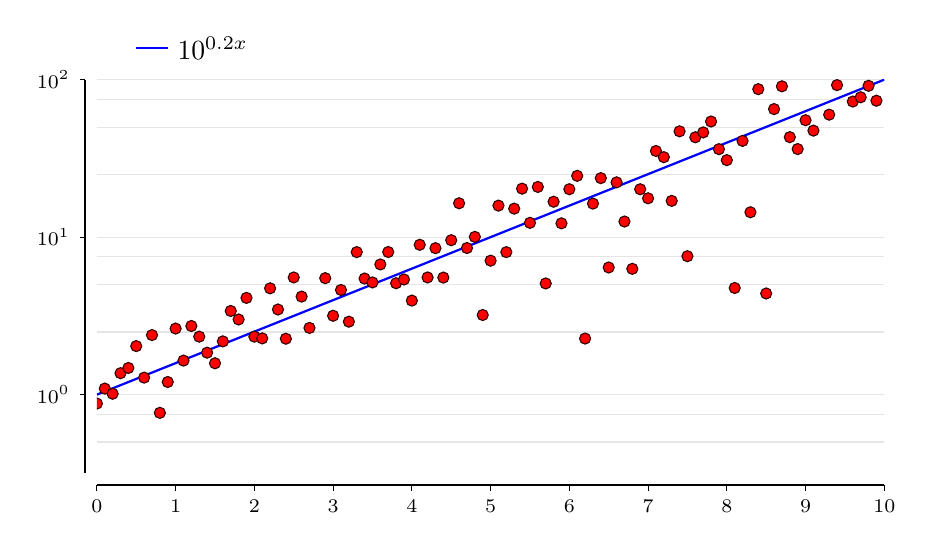
\begin{tikzpicture}[]
\begin{scope}[shift={(0.0,0.0)}]
\pgfsetxvec{\pgfpoint{1.0cm}{0cm}}
\pgfsetyvec{\pgfpoint{0cm}{2.0cm}}
\begin{scope}[shift={(0.0,0.5)}]
\begin{scope}[thick,black,fill=white]
\pgfpathmoveto{ \pgfpointadd{\pgfpointxy {0.0} {-0.5}} {\pgfpoint{0}{-0.15cm}} }
\pgfpathlineto{ \pgfpointadd{\pgfpointxy {10.0} {-0.5}} {\pgfpoint{0}{-0.15cm}} }
\pgfpathmoveto{ \pgfpointadd{\pgfpointxy {0.0} {-0.5}} {\pgfpoint{-0.15cm}{0}} }
\pgfpathlineto{ \pgfpointadd{\pgfpointxy {0.0} {2.0}} {\pgfpoint{-0.15cm}{0}} }
\pgfusepath{ stroke, }
\end{scope}
\begin{scope}[yshift=-0.15cm]
\draw[] [shift={(0.0,-0.5)}] (0,0) -- (0,-2pt) node[below]{ \scriptsize{\num[round-mode=places,round-precision=0]{0.0}}};
\draw[] [shift={(1.0,-0.5)}] (0,0) -- (0,-2pt) node[below]{ \scriptsize{\num[round-mode=places,round-precision=0]{1.0}}};
\draw[] [shift={(2.0,-0.5)}] (0,0) -- (0,-2pt) node[below]{ \scriptsize{\num[round-mode=places,round-precision=0]{2.0}}};
\draw[] [shift={(3.0,-0.5)}] (0,0) -- (0,-2pt) node[below]{ \scriptsize{\num[round-mode=places,round-precision=0]{3.0}}};
\draw[] [shift={(4.0,-0.5)}] (0,0) -- (0,-2pt) node[below]{ \scriptsize{\num[round-mode=places,round-precision=0]{4.0}}};
\draw[] [shift={(5.0,-0.5)}] (0,0) -- (0,-2pt) node[below]{ \scriptsize{\num[round-mode=places,round-precision=0]{5.0}}};
\draw[] [shift={(6.0,-0.5)}] (0,0) -- (0,-2pt) node[below]{ \scriptsize{\num[round-mode=places,round-precision=0]{6.0}}};
\draw[] [shift={(7.0,-0.5)}] (0,0) -- (0,-2pt) node[below]{ \scriptsize{\num[round-mode=places,round-precision=0]{7.0}}};
\draw[] [shift={(8.0,-0.5)}] (0,0) -- (0,-2pt) node[below]{ \scriptsize{\num[round-mode=places,round-precision=0]{8.0}}};
\draw[] [shift={(9.0,-0.5)}] (0,0) -- (0,-2pt) node[below]{ \scriptsize{\num[round-mode=places,round-precision=0]{9.0}}};
\draw[] [shift={(10.0,-0.5)}] (0,0) -- (0,-2pt) node[below]{ \scriptsize{\num[round-mode=places,round-precision=0]{10.0}}};
\end{scope}
\begin{scope}[xshift=-0.15cm]
\end{scope}
\end{scope}
\end{scope}
\pgfsetxvec{\pgfpoint{1cm}{0cm}}
\pgfsetyvec{\pgfpoint{0cm}{1cm}}
\begin{scope}[shift={(0.0,0.0)}]
\pgfsetxvec{\pgfpoint{1.0cm}{0cm}}
\pgfsetyvec{\pgfpoint{0cm}{2.0cm}}
\begin{scope}[shift={(0.0,0.5)}]
\begin{scope}[thin,gray!20!white]
\pgfpathmoveto{ \pgfpointxy {0.0} {-0.30102999566398114}}
\pgfpathlineto{ \pgfpointxy {10.0} {-0.30102999566398114}}
\pgfpathmoveto{ \pgfpointxy {0.0} {-0.12493873660829995}}
\pgfpathlineto{ \pgfpointxy {10.0} {-0.12493873660829995}}
\pgfpathmoveto{ \pgfpointxy {0.0} {0.0}}
\pgfpathlineto{ \pgfpointxy {10.0} {0.0}}
\pgfpathmoveto{ \pgfpointxy {0.0} {0.3979400086720376}}
\pgfpathlineto{ \pgfpointxy {10.0} {0.3979400086720376}}
\pgfpathmoveto{ \pgfpointxy {0.0} {0.6989700043360187}}
\pgfpathlineto{ \pgfpointxy {10.0} {0.6989700043360187}}
\pgfpathmoveto{ \pgfpointxy {0.0} {0.8750612633917}}
\pgfpathlineto{ \pgfpointxy {10.0} {0.8750612633917}}
\pgfpathmoveto{ \pgfpointxy {0.0} {1.0}}
\pgfpathlineto{ \pgfpointxy {10.0} {1.0}}
\pgfpathmoveto{ \pgfpointxy {0.0} {1.39794}}
\pgfpathlineto{ \pgfpointxy {10.0} {1.39794}}
\pgfpathmoveto{ \pgfpointxy {0.0} {1.69897}}
\pgfpathlineto{ \pgfpointxy {10.0} {1.69897}}
\pgfpathmoveto{ \pgfpointxy {0.0} {1.8750613}}
\pgfpathlineto{ \pgfpointxy {10.0} {1.8750613}}
\pgfpathmoveto{ \pgfpointxy {0.0} {2.0}}
\pgfpathlineto{ \pgfpointxy {10.0} {2.0}}
\pgfusepath{ stroke, }
\end{scope}
\end{scope}
\end{scope}
\pgfsetxvec{\pgfpoint{1cm}{0cm}}
\pgfsetyvec{\pgfpoint{0cm}{1cm}}
\begin{scope}[shift={(0.0,0.0)}]
\pgfsetxvec{\pgfpoint{1.0cm}{0cm}}
\pgfsetyvec{\pgfpoint{0cm}{2.0cm}}
\begin{scope}[shift={(0.0,0.5)}]
\begin{scope}[xshift=-0.15cm]
\draw[black] [shift={(0.0,0.0)}] (0,0) -- (-2pt,0) node[left]{ \scriptsize{$10^{0}$}};
\draw[black] [shift={(0.0,1.0)}] (0,0) -- (-2pt,0) node[left]{ \scriptsize{$10^{1}$}};
\draw[black] [shift={(0.0,2.0)}] (0,0) -- (-2pt,0) node[left]{ \scriptsize{$10^{2}$}};
\end{scope}
\end{scope}
\end{scope}
\pgfsetxvec{\pgfpoint{1cm}{0cm}}
\pgfsetyvec{\pgfpoint{0cm}{1cm}}
\begin{scope}[]
\pgfpathmoveto{ \pgfpointadd{\pgfpointxy {0.0} {0.0}} {\pgfpoint{0cm}{0cm}} }
\pgfpathlineto{ \pgfpointadd{\pgfpointxy {0.0} {0.0}} {\pgfpoint{10cm}{0cm}} }
\pgfpathlineto{ \pgfpointadd{\pgfpointxy {0.0} {0.0}} {\pgfpoint{10cm}{5cm}} }
\pgfpathlineto{ \pgfpointadd{\pgfpointxy {0.0} {0.0}} {\pgfpoint{0cm}{5cm}} }
\pgfpathclose
\pgfusepath{  clip, }
\begin{scope}[shift={(0.0,0.0)}]
\pgfsetxvec{\pgfpoint{1.0cm}{0cm}}
\pgfsetyvec{\pgfpoint{0cm}{2.0cm}}
\begin{scope}[shift={(0.0,0.5)}]
\begin{scope}[blue,thick]
\pgfpathmoveto{ \pgfpointxy {0.0} {0.0}}
\pgfpathlineto{ \pgfpointxy {0.1} {0.02000000000000003}}
\pgfpathlineto{ \pgfpointxy {0.2} {0.04000000000000003}}
\pgfpathlineto{ \pgfpointxy {0.3} {0.060000000000000026}}
\pgfpathlineto{ \pgfpointxy {0.4} {0.08}}
\pgfpathlineto{ \pgfpointxy {0.5} {0.10000000000000002}}
\pgfpathlineto{ \pgfpointxy {0.6} {0.11999999999999995}}
\pgfpathlineto{ \pgfpointxy {0.7} {0.13999999999999996}}
\pgfpathlineto{ \pgfpointxy {0.8} {0.16}}
\pgfpathlineto{ \pgfpointxy {0.9} {0.18}}
\pgfpathlineto{ \pgfpointxy {1.0} {0.20000000000000004}}
\pgfpathlineto{ \pgfpointxy {1.1} {0.21999999999999997}}
\pgfpathlineto{ \pgfpointxy {1.2} {0.23999999999999996}}
\pgfpathlineto{ \pgfpointxy {1.3} {0.25999999999999995}}
\pgfpathlineto{ \pgfpointxy {1.4} {0.2799999999999999}}
\pgfpathlineto{ \pgfpointxy {1.5} {0.3}}
\pgfpathlineto{ \pgfpointxy {1.6} {0.32}}
\pgfpathlineto{ \pgfpointxy {1.7} {0.33999999999999997}}
\pgfpathlineto{ \pgfpointxy {1.8} {0.36}}
\pgfpathlineto{ \pgfpointxy {1.9} {0.37999999999999995}}
\pgfpathlineto{ \pgfpointxy {2.0} {0.39999999999999997}}
\pgfpathlineto{ \pgfpointxy {2.1} {0.42000000000000004}}
\pgfpathlineto{ \pgfpointxy {2.2} {0.43999999999999995}}
\pgfpathlineto{ \pgfpointxy {2.3} {0.4599999999999999}}
\pgfpathlineto{ \pgfpointxy {2.4} {0.4799999999999999}}
\pgfpathlineto{ \pgfpointxy {2.5} {0.5}}
\pgfpathlineto{ \pgfpointxy {2.6} {0.52}}
\pgfpathlineto{ \pgfpointxy {2.7} {0.54}}
\pgfpathlineto{ \pgfpointxy {2.8} {0.5599999999999999}}
\pgfpathlineto{ \pgfpointxy {2.9} {0.5799999999999998}}
\pgfpathlineto{ \pgfpointxy {3.0} {0.6000000000000001}}
\pgfpathlineto{ \pgfpointxy {3.1} {0.6199999999999999}}
\pgfpathlineto{ \pgfpointxy {3.2} {0.64}}
\pgfpathlineto{ \pgfpointxy {3.3} {0.66}}
\pgfpathlineto{ \pgfpointxy {3.4} {0.68}}
\pgfpathlineto{ \pgfpointxy {3.5} {0.7000000000000001}}
\pgfpathlineto{ \pgfpointxy {3.6} {0.72}}
\pgfpathlineto{ \pgfpointxy {3.7} {0.7400000000000001}}
\pgfpathlineto{ \pgfpointxy {3.8} {0.76}}
\pgfpathlineto{ \pgfpointxy {3.9} {0.78}}
\pgfpathlineto{ \pgfpointxy {4.0} {0.7999999999999999}}
\pgfpathlineto{ \pgfpointxy {4.1} {0.82}}
\pgfpathlineto{ \pgfpointxy {4.2} {0.8400000000000001}}
\pgfpathlineto{ \pgfpointxy {4.3} {0.86}}
\pgfpathlineto{ \pgfpointxy {4.4} {0.8800000000000002}}
\pgfpathlineto{ \pgfpointxy {4.5} {0.9}}
\pgfpathlineto{ \pgfpointxy {4.6} {0.92}}
\pgfpathlineto{ \pgfpointxy {4.7} {0.94}}
\pgfpathlineto{ \pgfpointxy {4.8} {0.9599999999999999}}
\pgfpathlineto{ \pgfpointxy {4.9} {0.9800000000000001}}
\pgfpathlineto{ \pgfpointxy {5.0} {1.0}}
\pgfpathlineto{ \pgfpointxy {5.1} {1.02}}
\pgfpathlineto{ \pgfpointxy {5.2} {1.04}}
\pgfpathlineto{ \pgfpointxy {5.3} {1.06}}
\pgfpathlineto{ \pgfpointxy {5.4} {1.08}}
\pgfpathlineto{ \pgfpointxy {5.5} {1.0999999999999999}}
\pgfpathlineto{ \pgfpointxy {5.6} {1.1199999999999999}}
\pgfpathlineto{ \pgfpointxy {5.7} {1.1400000000000001}}
\pgfpathlineto{ \pgfpointxy {5.8} {1.1599999999999997}}
\pgfpathlineto{ \pgfpointxy {5.9} {1.18}}
\pgfpathlineto{ \pgfpointxy {6.0} {1.2000000000000002}}
\pgfpathlineto{ \pgfpointxy {6.1} {1.22}}
\pgfpathlineto{ \pgfpointxy {6.2} {1.2400000000000002}}
\pgfpathlineto{ \pgfpointxy {6.3} {1.26}}
\pgfpathlineto{ \pgfpointxy {6.4} {1.28}}
\pgfpathlineto{ \pgfpointxy {6.5} {1.3}}
\pgfpathlineto{ \pgfpointxy {6.6} {1.32}}
\pgfpathlineto{ \pgfpointxy {6.7} {1.3399999999999999}}
\pgfpathlineto{ \pgfpointxy {6.8} {1.36}}
\pgfpathlineto{ \pgfpointxy {6.9} {1.38}}
\pgfpathlineto{ \pgfpointxy {7.0} {1.4000000000000001}}
\pgfpathlineto{ \pgfpointxy {7.1} {1.42}}
\pgfpathlineto{ \pgfpointxy {7.2} {1.44}}
\pgfpathlineto{ \pgfpointxy {7.3} {1.46}}
\pgfpathlineto{ \pgfpointxy {7.4} {1.4800000000000002}}
\pgfpathlineto{ \pgfpointxy {7.5} {1.4999999999999998}}
\pgfpathlineto{ \pgfpointxy {7.6} {1.52}}
\pgfpathlineto{ \pgfpointxy {7.7} {1.5399999999999998}}
\pgfpathlineto{ \pgfpointxy {7.8} {1.56}}
\pgfpathlineto{ \pgfpointxy {7.9} {1.5799999999999998}}
\pgfpathlineto{ \pgfpointxy {8.0} {1.5999999999999999}}
\pgfpathlineto{ \pgfpointxy {8.1} {1.62}}
\pgfpathlineto{ \pgfpointxy {8.2} {1.64}}
\pgfpathlineto{ \pgfpointxy {8.3} {1.6600000000000001}}
\pgfpathlineto{ \pgfpointxy {8.4} {1.6800000000000002}}
\pgfpathlineto{ \pgfpointxy {8.5} {1.7000000000000004}}
\pgfpathlineto{ \pgfpointxy {8.6} {1.72}}
\pgfpathlineto{ \pgfpointxy {8.7} {1.74}}
\pgfpathlineto{ \pgfpointxy {8.8} {1.7600000000000005}}
\pgfpathlineto{ \pgfpointxy {8.9} {1.7800000000000002}}
\pgfpathlineto{ \pgfpointxy {9.0} {1.7999999999999998}}
\pgfpathlineto{ \pgfpointxy {9.1} {1.82}}
\pgfpathlineto{ \pgfpointxy {9.2} {1.8399999999999996}}
\pgfpathlineto{ \pgfpointxy {9.3} {1.86}}
\pgfpathlineto{ \pgfpointxy {9.4} {1.8800000000000003}}
\pgfpathlineto{ \pgfpointxy {9.5} {1.9000000000000001}}
\pgfpathlineto{ \pgfpointxy {9.6} {1.9199999999999997}}
\pgfpathlineto{ \pgfpointxy {9.7} {1.94}}
\pgfpathlineto{ \pgfpointxy {9.8} {1.9600000000000002}}
\pgfpathlineto{ \pgfpointxy {9.9} {1.9800000000000002}}
\pgfpathlineto{ \pgfpointxy {10.0} {2.0}}
\pgfusepath{ stroke, }
\end{scope}
\end{scope}
\end{scope}
\pgfsetxvec{\pgfpoint{1cm}{0cm}}
\pgfsetyvec{\pgfpoint{0cm}{1cm}}
\end{scope}
\draw[blue,thick] (0.5,5.3999999999999995) -- (0.9,5.3999999999999995);
\draw[opacity=0.0,white] (0.5,5.5) -- (0.5,5.3);
\node at (0.9,5.3999999999999995) [right,] {$10^{0.2 x}$};
\begin{scope}[]
\pgfpathmoveto{ \pgfpointadd{\pgfpointxy {0.0} {0.0}} {\pgfpoint{0cm}{0cm}} }
\pgfpathlineto{ \pgfpointadd{\pgfpointxy {0.0} {0.0}} {\pgfpoint{10cm}{0cm}} }
\pgfpathlineto{ \pgfpointadd{\pgfpointxy {0.0} {0.0}} {\pgfpoint{10cm}{5cm}} }
\pgfpathlineto{ \pgfpointadd{\pgfpointxy {0.0} {0.0}} {\pgfpoint{0cm}{5cm}} }
\pgfpathclose
\pgfusepath{  clip, }
\begin{scope}[shift={(0.0,0.0)}]
\pgfsetxvec{\pgfpoint{1.0cm}{0cm}}
\pgfsetyvec{\pgfpoint{0cm}{2.0cm}}
\begin{scope}[shift={(0.0,0.5)}]
\node at (0.0,-0.05655646582801225) [fill=red,draw=red!20!black,circle,inner sep=0.0pt,minimum width =4.0pt,minimum height=4.0pt] {};
\node at (0.1,0.03829591574090131) [fill=red,draw=red!20!black,circle,inner sep=0.0pt,minimum width =4.0pt,minimum height=4.0pt] {};
\node at (0.2,0.005494579890783447) [fill=red,draw=red!20!black,circle,inner sep=0.0pt,minimum width =4.0pt,minimum height=4.0pt] {};
\node at (0.30000000000000004,0.13606029860533428) [fill=red,draw=red!20!black,circle,inner sep=0.0pt,minimum width =4.0pt,minimum height=4.0pt] {};
\node at (0.4,0.16940270397173854) [fill=red,draw=red!20!black,circle,inner sep=0.0pt,minimum width =4.0pt,minimum height=4.0pt] {};
\node at (0.5,0.3080621138446519) [fill=red,draw=red!20!black,circle,inner sep=0.0pt,minimum width =4.0pt,minimum height=4.0pt] {};
\node at (0.6000000000000001,0.10789070053997156) [fill=red,draw=red!20!black,circle,inner sep=0.0pt,minimum width =4.0pt,minimum height=4.0pt] {};
\node at (0.7000000000000001,0.3780115548622542) [fill=red,draw=red!20!black,circle,inner sep=0.0pt,minimum width =4.0pt,minimum height=4.0pt] {};
\node at (0.8,-0.11578730643678818) [fill=red,draw=red!20!black,circle,inner sep=0.0pt,minimum width =4.0pt,minimum height=4.0pt] {};
\node at (0.9,0.08016098129452058) [fill=red,draw=red!20!black,circle,inner sep=0.0pt,minimum width =4.0pt,minimum height=4.0pt] {};
\node at (1.0,0.41950289216887976) [fill=red,draw=red!20!black,circle,inner sep=0.0pt,minimum width =4.0pt,minimum height=4.0pt] {};
\node at (1.1,0.21591557764141783) [fill=red,draw=red!20!black,circle,inner sep=0.0pt,minimum width =4.0pt,minimum height=4.0pt] {};
\node at (1.2000000000000002,0.4357386807838701) [fill=red,draw=red!20!black,circle,inner sep=0.0pt,minimum width =4.0pt,minimum height=4.0pt] {};
\node at (1.3,0.36801370411927165) [fill=red,draw=red!20!black,circle,inner sep=0.0pt,minimum width =4.0pt,minimum height=4.0pt] {};
\node at (1.4000000000000001,0.2664005831868513) [fill=red,draw=red!20!black,circle,inner sep=0.0pt,minimum width =4.0pt,minimum height=4.0pt] {};
\node at (1.5,0.19909745512432617) [fill=red,draw=red!20!black,circle,inner sep=0.0pt,minimum width =4.0pt,minimum height=4.0pt] {};
\node at (1.6,0.3380603478984181) [fill=red,draw=red!20!black,circle,inner sep=0.0pt,minimum width =4.0pt,minimum height=4.0pt] {};
\node at (1.7000000000000002,0.531157710583475) [fill=red,draw=red!20!black,circle,inner sep=0.0pt,minimum width =4.0pt,minimum height=4.0pt] {};
\node at (1.8,0.4772868574213) [fill=red,draw=red!20!black,circle,inner sep=0.0pt,minimum width =4.0pt,minimum height=4.0pt] {};
\node at (1.9000000000000001,0.6141565122658951) [fill=red,draw=red!20!black,circle,inner sep=0.0pt,minimum width =4.0pt,minimum height=4.0pt] {};
\node at (2.0,0.36806307387117665) [fill=red,draw=red!20!black,circle,inner sep=0.0pt,minimum width =4.0pt,minimum height=4.0pt] {};
\node at (2.1,0.3571163681792146) [fill=red,draw=red!20!black,circle,inner sep=0.0pt,minimum width =4.0pt,minimum height=4.0pt] {};
\node at (2.2,0.6749426170775258) [fill=red,draw=red!20!black,circle,inner sep=0.0pt,minimum width =4.0pt,minimum height=4.0pt] {};
\node at (2.3000000000000003,0.5404661968455311) [fill=red,draw=red!20!black,circle,inner sep=0.0pt,minimum width =4.0pt,minimum height=4.0pt] {};
\node at (2.4000000000000004,0.35499669954094437) [fill=red,draw=red!20!black,circle,inner sep=0.0pt,minimum width =4.0pt,minimum height=4.0pt] {};
\node at (2.5,0.7439934379857392) [fill=red,draw=red!20!black,circle,inner sep=0.0pt,minimum width =4.0pt,minimum height=4.0pt] {};
\node at (2.6,0.6224528393339267) [fill=red,draw=red!20!black,circle,inner sep=0.0pt,minimum width =4.0pt,minimum height=4.0pt] {};
\node at (2.7,0.42351922522798036) [fill=red,draw=red!20!black,circle,inner sep=0.0pt,minimum width =4.0pt,minimum height=4.0pt] {};
\node at (2.8000000000000003,-0.5678621310551657) [fill=red,draw=red!20!black,circle,inner sep=0.0pt,minimum width =4.0pt,minimum height=4.0pt] {};
\node at (2.9000000000000004,0.7394702411330144) [fill=red,draw=red!20!black,circle,inner sep=0.0pt,minimum width =4.0pt,minimum height=4.0pt] {};
\node at (3.0,0.5006629450756376) [fill=red,draw=red!20!black,circle,inner sep=0.0pt,minimum width =4.0pt,minimum height=4.0pt] {};
\node at (3.1,0.6644304581377032) [fill=red,draw=red!20!black,circle,inner sep=0.0pt,minimum width =4.0pt,minimum height=4.0pt] {};
\node at (3.2,0.4632446362928611) [fill=red,draw=red!20!black,circle,inner sep=0.0pt,minimum width =4.0pt,minimum height=4.0pt] {};
\node at (3.3000000000000003,0.9048460025309718) [fill=red,draw=red!20!black,circle,inner sep=0.0pt,minimum width =4.0pt,minimum height=4.0pt] {};
\node at (3.4000000000000004,0.737162751592065) [fill=red,draw=red!20!black,circle,inner sep=0.0pt,minimum width =4.0pt,minimum height=4.0pt] {};
\node at (3.5,0.7124004875731801) [fill=red,draw=red!20!black,circle,inner sep=0.0pt,minimum width =4.0pt,minimum height=4.0pt] {};
\node at (3.6,0.8267239717208485) [fill=red,draw=red!20!black,circle,inner sep=0.0pt,minimum width =4.0pt,minimum height=4.0pt] {};
\node at (3.7,0.9054904810520419) [fill=red,draw=red!20!black,circle,inner sep=0.0pt,minimum width =4.0pt,minimum height=4.0pt] {};
\node at (3.8000000000000003,0.7072953375637681) [fill=red,draw=red!20!black,circle,inner sep=0.0pt,minimum width =4.0pt,minimum height=4.0pt] {};
\node at (3.9000000000000004,0.7312013797919721) [fill=red,draw=red!20!black,circle,inner sep=0.0pt,minimum width =4.0pt,minimum height=4.0pt] {};
\node at (4.0,0.5970431271310029) [fill=red,draw=red!20!black,circle,inner sep=0.0pt,minimum width =4.0pt,minimum height=4.0pt] {};
\node at (4.1000000000000005,0.9513514688078052) [fill=red,draw=red!20!black,circle,inner sep=0.0pt,minimum width =4.0pt,minimum height=4.0pt] {};
\node at (4.2,0.7439875554668108) [fill=red,draw=red!20!black,circle,inner sep=0.0pt,minimum width =4.0pt,minimum height=4.0pt] {};
\node at (4.3,0.929864670444076) [fill=red,draw=red!20!black,circle,inner sep=0.0pt,minimum width =4.0pt,minimum height=4.0pt] {};
\node at (4.4,0.7431167286123636) [fill=red,draw=red!20!black,circle,inner sep=0.0pt,minimum width =4.0pt,minimum height=4.0pt] {};
\node at (4.5,0.9804575672044229) [fill=red,draw=red!20!black,circle,inner sep=0.0pt,minimum width =4.0pt,minimum height=4.0pt] {};
\node at (4.6000000000000005,1.2150936390280944) [fill=red,draw=red!20!black,circle,inner sep=0.0pt,minimum width =4.0pt,minimum height=4.0pt] {};
\node at (4.7,0.9307940469827529) [fill=red,draw=red!20!black,circle,inner sep=0.0pt,minimum width =4.0pt,minimum height=4.0pt] {};
\node at (4.800000000000001,1.0016452523969082) [fill=red,draw=red!20!black,circle,inner sep=0.0pt,minimum width =4.0pt,minimum height=4.0pt] {};
\node at (4.9,0.5055130907941692) [fill=red,draw=red!20!black,circle,inner sep=0.0pt,minimum width =4.0pt,minimum height=4.0pt] {};
\node at (5.0,0.850510923438997) [fill=red,draw=red!20!black,circle,inner sep=0.0pt,minimum width =4.0pt,minimum height=4.0pt] {};
\node at (5.1000000000000005,1.2000846461256118) [fill=red,draw=red!20!black,circle,inner sep=0.0pt,minimum width =4.0pt,minimum height=4.0pt] {};
\node at (5.2,0.9046256526556337) [fill=red,draw=red!20!black,circle,inner sep=0.0pt,minimum width =4.0pt,minimum height=4.0pt] {};
\node at (5.300000000000001,1.1808754588468675) [fill=red,draw=red!20!black,circle,inner sep=0.0pt,minimum width =4.0pt,minimum height=4.0pt] {};
\node at (5.4,1.3078549808502942) [fill=red,draw=red!20!black,circle,inner sep=0.0pt,minimum width =4.0pt,minimum height=4.0pt] {};
\node at (5.5,1.090709148798597) [fill=red,draw=red!20!black,circle,inner sep=0.0pt,minimum width =4.0pt,minimum height=4.0pt] {};
\node at (5.6000000000000005,1.3187378600154605) [fill=red,draw=red!20!black,circle,inner sep=0.0pt,minimum width =4.0pt,minimum height=4.0pt] {};
\node at (5.7,0.705893533428918) [fill=red,draw=red!20!black,circle,inner sep=0.0pt,minimum width =4.0pt,minimum height=4.0pt] {};
\node at (5.800000000000001,1.224721577326744) [fill=red,draw=red!20!black,circle,inner sep=0.0pt,minimum width =4.0pt,minimum height=4.0pt] {};
\node at (5.9,1.0877428363179202) [fill=red,draw=red!20!black,circle,inner sep=0.0pt,minimum width =4.0pt,minimum height=4.0pt] {};
\node at (6.0,1.3041991748731847) [fill=red,draw=red!20!black,circle,inner sep=0.0pt,minimum width =4.0pt,minimum height=4.0pt] {};
\node at (6.1000000000000005,1.389156303329451) [fill=red,draw=red!20!black,circle,inner sep=0.0pt,minimum width =4.0pt,minimum height=4.0pt] {};
\node at (6.2,0.35602083362776626) [fill=red,draw=red!20!black,circle,inner sep=0.0pt,minimum width =4.0pt,minimum height=4.0pt] {};
\node at (6.300000000000001,1.2130492931392152) [fill=red,draw=red!20!black,circle,inner sep=0.0pt,minimum width =4.0pt,minimum height=4.0pt] {};
\node at (6.4,1.374630337513968) [fill=red,draw=red!20!black,circle,inner sep=0.0pt,minimum width =4.0pt,minimum height=4.0pt] {};
\node at (6.5,0.8073578037994915) [fill=red,draw=red!20!black,circle,inner sep=0.0pt,minimum width =4.0pt,minimum height=4.0pt] {};
\node at (6.6000000000000005,1.347901165355187) [fill=red,draw=red!20!black,circle,inner sep=0.0pt,minimum width =4.0pt,minimum height=4.0pt] {};
\node at (6.7,1.0990628482896374) [fill=red,draw=red!20!black,circle,inner sep=0.0pt,minimum width =4.0pt,minimum height=4.0pt] {};
\node at (6.800000000000001,0.7986326396455822) [fill=red,draw=red!20!black,circle,inner sep=0.0pt,minimum width =4.0pt,minimum height=4.0pt] {};
\node at (6.9,1.3040872989057122) [fill=red,draw=red!20!black,circle,inner sep=0.0pt,minimum width =4.0pt,minimum height=4.0pt] {};
\node at (7.0,1.246516242262846) [fill=red,draw=red!20!black,circle,inner sep=0.0pt,minimum width =4.0pt,minimum height=4.0pt] {};
\node at (7.1000000000000005,1.5470692247483087) [fill=red,draw=red!20!black,circle,inner sep=0.0pt,minimum width =4.0pt,minimum height=4.0pt] {};
\node at (7.2,1.5077329677697537) [fill=red,draw=red!20!black,circle,inner sep=0.0pt,minimum width =4.0pt,minimum height=4.0pt] {};
\node at (7.300000000000001,1.2302390953741786) [fill=red,draw=red!20!black,circle,inner sep=0.0pt,minimum width =4.0pt,minimum height=4.0pt] {};
\node at (7.4,1.6719734294927038) [fill=red,draw=red!20!black,circle,inner sep=0.0pt,minimum width =4.0pt,minimum height=4.0pt] {};
\node at (7.5,0.87890639968303) [fill=red,draw=red!20!black,circle,inner sep=0.0pt,minimum width =4.0pt,minimum height=4.0pt] {};
\node at (7.6000000000000005,1.6340679102969264) [fill=red,draw=red!20!black,circle,inner sep=0.0pt,minimum width =4.0pt,minimum height=4.0pt] {};
\node at (7.7,1.6648720475290937) [fill=red,draw=red!20!black,circle,inner sep=0.0pt,minimum width =4.0pt,minimum height=4.0pt] {};
\node at (7.800000000000001,1.734307118831054) [fill=red,draw=red!20!black,circle,inner sep=0.0pt,minimum width =4.0pt,minimum height=4.0pt] {};
\node at (7.9,1.5585744226850993) [fill=red,draw=red!20!black,circle,inner sep=0.0pt,minimum width =4.0pt,minimum height=4.0pt] {};
\node at (8.0,1.4889741740395956) [fill=red,draw=red!20!black,circle,inner sep=0.0pt,minimum width =4.0pt,minimum height=4.0pt] {};
\node at (8.1,0.677105072837783) [fill=red,draw=red!20!black,circle,inner sep=0.0pt,minimum width =4.0pt,minimum height=4.0pt] {};
\node at (8.200000000000001,1.6109822607186988) [fill=red,draw=red!20!black,circle,inner sep=0.0pt,minimum width =4.0pt,minimum height=4.0pt] {};
\node at (8.3,1.157911069016338) [fill=red,draw=red!20!black,circle,inner sep=0.0pt,minimum width =4.0pt,minimum height=4.0pt] {};
\node at (8.4,1.9396146435911559) [fill=red,draw=red!20!black,circle,inner sep=0.0pt,minimum width =4.0pt,minimum height=4.0pt] {};
\node at (8.5,0.6421805236319593) [fill=red,draw=red!20!black,circle,inner sep=0.0pt,minimum width =4.0pt,minimum height=4.0pt] {};
\node at (8.6,1.8131091877639949) [fill=red,draw=red!20!black,circle,inner sep=0.0pt,minimum width =4.0pt,minimum height=4.0pt] {};
\node at (8.700000000000001,1.9576666164521146) [fill=red,draw=red!20!black,circle,inner sep=0.0pt,minimum width =4.0pt,minimum height=4.0pt] {};
\node at (8.8,1.6348491176640936) [fill=red,draw=red!20!black,circle,inner sep=0.0pt,minimum width =4.0pt,minimum height=4.0pt] {};
\node at (8.9,1.5593021554482611) [fill=red,draw=red!20!black,circle,inner sep=0.0pt,minimum width =4.0pt,minimum height=4.0pt] {};
\node at (9.0,1.7424758281753363) [fill=red,draw=red!20!black,circle,inner sep=0.0pt,minimum width =4.0pt,minimum height=4.0pt] {};
\node at (9.1,1.6763394220498835) [fill=red,draw=red!20!black,circle,inner sep=0.0pt,minimum width =4.0pt,minimum height=4.0pt] {};
\node at (9.200000000000001,2.0844817180369457) [fill=red,draw=red!20!black,circle,inner sep=0.0pt,minimum width =4.0pt,minimum height=4.0pt] {};
\node at (9.3,1.7777238272450422) [fill=red,draw=red!20!black,circle,inner sep=0.0pt,minimum width =4.0pt,minimum height=4.0pt] {};
\node at (9.4,1.9653882584595352) [fill=red,draw=red!20!black,circle,inner sep=0.0pt,minimum width =4.0pt,minimum height=4.0pt] {};
\node at (9.5,2.0754884160317757) [fill=red,draw=red!20!black,circle,inner sep=0.0pt,minimum width =4.0pt,minimum height=4.0pt] {};
\node at (9.600000000000001,1.8610028542269121) [fill=red,draw=red!20!black,circle,inner sep=0.0pt,minimum width =4.0pt,minimum height=4.0pt] {};
\node at (9.700000000000001,1.8881376634286924) [fill=red,draw=red!20!black,circle,inner sep=0.0pt,minimum width =4.0pt,minimum height=4.0pt] {};
\node at (9.8,1.9609027778880368) [fill=red,draw=red!20!black,circle,inner sep=0.0pt,minimum width =4.0pt,minimum height=4.0pt] {};
\node at (9.9,1.8662163547838537) [fill=red,draw=red!20!black,circle,inner sep=0.0pt,minimum width =4.0pt,minimum height=4.0pt] {};
\node at (10.0,2.062978346280785) [fill=red,draw=red!20!black,circle,inner sep=0.0pt,minimum width =4.0pt,minimum height=4.0pt] {};
\end{scope}
\end{scope}
\pgfsetxvec{\pgfpoint{1cm}{0cm}}
\pgfsetyvec{\pgfpoint{0cm}{1cm}}
\end{scope}
\end{tikzpicture}
\end{document}

  \caption{ Log scale with sub ticks. The log scaling is done explicitly, not using tikz.}
\end{figure}

\end{document}
  
%%% Local Variables: 
%%% mode: latex
%%% TeX-master: t
%%% End: 
